\documentclass{ut-thesis}

% Packages
\usepackage[colorlinks,
            urlcolor=blue,
            linkcolor=blue,
            citecolor=blue]
            {hyperref} % for links
\usepackage[backend=biber,
            style=authoryear]
            {biblatex} % for references
\usepackage{graphicx} % for embedding graphics
\usepackage{booktabs} % for pretty tables
\usepackage{amsmath}
% \usepackage{natbib}

% Commands
% Universal macros
\newcommand{\james}[1]{ \textbf{{\textcolor{red} #1 }} }

% Spacing
\newlength{\halftextwidth}
\setlength{\halftextwidth}{0.5\textwidth}

% Units
\newcommand{\Msun}{M$_{\odot}$}

% Ch1

% Ch2
\newcommand{\solar}{\emph{Solar}}
\newcommand{\survey}{\emph{Survey}}
\newcommand\degr{\hbox{$^\circ$}}

% Ch3

% Bibliography
\newcommand\aap{A\&A}                % Astronomy and Astrophysics
\let\astap=\aap                          % alternative shortcut
\newcommand\aapr{A\&ARv}             % Astronomy and Astrophysics Review (the)
\newcommand\aaps{A\&AS}              % Astronomy and Astrophysics Supplement Series
\newcommand\actaa{Acta Astron.}      % Acta Astronomica
\newcommand\afz{Afz}                 % Astrofizika
\newcommand\aj{AJ}                   % Astronomical Journal (the)
\newcommand\ao{Appl. Opt.}           % Applied Optics
\let\applopt=\ao                         % alternative shortcut
\newcommand\aplett{Astrophys.~Lett.} % Astrophysics Letters
\newcommand\apj{ApJ}                 % Astrophysical Journal
\newcommand\apjl{ApJ}                % Astrophysical Journal, Letters
\let\apjlett=\apjl                       % alternative shortcut
\newcommand\apjs{ApJS}               % Astrophysical Journal, Supplement
\let\apjsupp=\apjs                       % alternative shortcut
% The following journal does not appear to exist! Disabled.
%\newcommand\apspr{Astrophys.~Space~Phys.~Res.} % Astrophysics Space Physics Research
\newcommand\apss{Ap\&SS}             % Astrophysics and Space Science
\newcommand\araa{ARA\&A}             % Annual Review of Astronomy and Astrophysics
\newcommand\arep{Astron. Rep.}       % Astronomy Reports
\newcommand\aspc{ASP Conf. Ser.}     % ASP Conference Series
\newcommand\azh{Azh}                 % Astronomicheskii Zhurnal
\newcommand\baas{BAAS}               % Bulletin of the American Astronomical Society
\newcommand\bac{Bull. Astron. Inst. Czechoslovakia} % Bulletin of the Astronomical Institutes of Czechoslovakia 
\newcommand\bain{Bull. Astron. Inst. Netherlands} % Bulletin Astronomical Institute of the Netherlands
\newcommand\caa{Chinese Astron. Astrophys.} % Chinese Astronomy and Astrophysics
\newcommand\cjaa{Chinese J.~Astron. Astrophys.} % Chinese Journal of Astronomy and Astrophysics
\newcommand\fcp{Fundamentals Cosmic Phys.}  % Fundamentals of Cosmic Physics
\newcommand\gca{Geochimica Cosmochimica Acta}   % Geochimica Cosmochimica Acta
\newcommand\grl{Geophys. Res. Lett.} % Geophysics Research Letters
\newcommand\iaucirc{IAU~Circ.}       % IAU Cirulars
\newcommand\icarus{Icarus}           % Icarus
\newcommand\japa{J.~Astrophys. Astron.} % Journal of Astrophysics and Astronomy
\newcommand\jcap{J.~Cosmology Astropart. Phys.} % Journal of Cosmology and Astroparticle Physics
\newcommand\jcp{J.~Chem.~Phys.}      % Journal of Chemical Physics
\newcommand\jgr{J.~Geophys.~Res.}    % Journal of Geophysics Research
\newcommand\jqsrt{J.~Quant. Spectrosc. Radiative Transfer} % Journal of Quantitiative Spectroscopy and Radiative Transfer
\newcommand\jrasc{J.~R.~Astron. Soc. Canada} % Journal of the RAS of Canada
\newcommand\memras{Mem.~RAS}         % Memoirs of the RAS
\newcommand\memsai{Mem. Soc. Astron. Italiana} % Memoire della Societa Astronomica Italiana
\newcommand\mnassa{MNASSA}           % Monthly Notes of the Astronomical Society of Southern Africa
\newcommand\mnras{MNRAS}             % Monthly Notices of the Royal Astronomical Society
\newcommand\na{New~Astron.}          % New Astronomy
\newcommand\nar{New~Astron.~Rev.}    % New Astronomy Review
\newcommand\nat{Nature}              % Nature
\newcommand\nphysa{Nuclear Phys.~A}  % Nuclear Physics A
\newcommand\pra{Phys. Rev.~A}        % Physical Review A: General Physics
\newcommand\prb{Phys. Rev.~B}        % Physical Review B: Solid State
\newcommand\prc{Phys. Rev.~C}        % Physical Review C
\newcommand\prd{Phys. Rev.~D}        % Physical Review D
\newcommand\pre{Phys. Rev.~E}        % Physical Review E
\newcommand\prl{Phys. Rev.~Lett.}    % Physical Review Letters
\newcommand\pasa{Publ. Astron. Soc. Australia}  % Publications of the Astronomical Society of Australia
\newcommand\pasp{PASP}               % Publications of the Astronomical Society of the Pacific
\newcommand\pasj{PASJ}               % Publications of the Astronomical Society of Japan
\newcommand\physrep{Phys.~Rep.}      % Physics Reports
\newcommand\physscr{Phys.~Scr.}      % Physica Scripta
\newcommand\planss{Planet. Space~Sci.} % Planetary Space Science
\newcommand\procspie{Proc.~SPIE}     % Proceedings of the Society of Photo-Optical Instrumentation Engineers
\newcommand\rmxaa{Rev. Mex. Astron. Astrofis.} % Revista Mexicana de Astronomia y Astrofisica
\newcommand\qjras{QJRAS}             % Quarterly Journal of the RAS
\newcommand\sci{Science}             % Science
\newcommand\skytel{Sky \& Telesc.}   % Sky and Telescope
\newcommand\solphys{Sol.~Phys.}      % Solar Physics
\newcommand\sovast{Soviet~Ast.}      % Soviet Astronomy (aka Astronomy Reports)
\newcommand\ssr{Space Sci. Rev.}     % Space Science Reviews
\newcommand\zap{Z.~Astrophys.}       % Zeitschrift fuer Astrophysik

% Personal information
\author{James Martin Mackay Lane}
\title{On the use of distribution functions for the study of the Milky Way stellar halo in the \textit{Gaia} era}
\degree{Doctor of Philosophy}
\gradyear{2024}
\department{Astronomy \& Astrophysics}

% reference database
\addbibresource{main.bib}

% Begin
\begin{document}

% Frontmatter
\frontmatter
\maketitle

% Abstract
\begin{abstract}
    \begin{abstract}
    Disk galaxies, such as our own Milky Way, populate the entire extent of the observable Universe and constitute its most fundamental building blocks. Among the many hallowed endeavours of modern astronomy is the cultivation of a deep and holistic understanding of how these galaxies form, grow, and evolve. The stellar halo of the Milky Way hosts the fossil remnants of past accretion events, reflecting the habit of the Milky Way to devour smaller nearby galaxies over cosmic timescales. Such accretion episodes are among the most formative events experienced by the Milky Way, contributing both to its genesis at early times as well as subsequent growth and evolution. Among the most important accreted stellar population in the halo is \textit{Gaia}-Sausage/Enceladus, the remnant of a substantial ancient merger event. Distribution functions are mathematical models for the phase space distribution of stellar populations, and are useful tools for the study of stellar halo populations. This thesis demonstrates work done to integrate the use of distribution functions into the study of the stellar halo, and the accretion remnants which largely comprise it, in the era of new data from the \textit{Gaia Space Telescope} and large ground-based spectroscopic surveys.

    Three projects are presented which work towards the development of a better understanding regarding the use of distribution functions. First, we employ distribution functions to construct data-driven models of the Milky Way stellar halo and investigate their properties. Second, we use distribution functions to aid in fitting density profiles to the \textit{Gaia}-Sausage/Enceladus remnant; upon determining its mass, we find it to be far less than previously thought. Third, we assess the applicability of a wide range of distribution function models by testing them on simulated merger remnants in Milky Way analogs found in the IllustrisTNG simulation. Among our key findings are: that it is crucial to consider selection effects carefully when searching for stellar halo remnants and other populations; that the \textit{Gaia}-Sausage/Enceladus remnant was likely deposited during a minor merger; and that it is probably best modeled using combinations of Osipkov-Merritt distribution functions in future studies. The principal conclusion of this thesis is that distribution functions can, and should, play a central role in the modelling of the stellar halo, as we seek to learn more about the formation and evolution of the Milky Way in the \textit{Gaia} era. 
\end{abstract}
\end{abstract}

% Dedication
\begin{dedication}
    For my grandfather, Bruce Mackay
\end{dedication}

% Acknowledgements
\begin{acknowledgements}
    \begin{itemize}
        \item Haley
        \item Mom and dad
        \item Carmen and Warren
        \item Academics: Jo, Ted, Bob, Suresh, Helen, Doug, Steve, Mike, Kim, Julio
        \item Friends: Mitch, Adam, Theron, Nick, Mike...
        \item Pets: Java, Phoebe, Zoe
        \item Inspirations: NDGT, Vsauce, Sixty symbols, 
    \end{itemize}
\end{acknowledgements}

% Lists
\tableofcontents
\listoftables
\listoffigures

\mainmatter

% \setcounter{chapter}{0}

% Chapter 1 - Introduction
\chapter{Introduction}

% I set the stage in this thesis with a look at the history of the study of Galaxies throughout the Universe. I then move on to the Milky Way in particular, and emphasize how its study has informed our understanding more broadly. Finally, I will summarize the main discoveries which have occurred in the \textit{Gaia} era, some being unexpected, and some validating or disproving past hypotheses.

\section{Galaxies in the \texorpdfstring{$\Lambda$CDM}{LambdaCDM} paradigm}

I begin this introduction with a look at the broadest cosmological scales, to attempt to contextualize the fundamental unit of the cosmos: the galaxy, within the greater whole of which it is a part.


\section{A brief history of the Milky Way}

In this chapter I outline the history of our understanding of the structure and properties of the Milky Way up to the first \textit{Gaia} data release. This body of knowledge also encompasses much of theory about the formation and evolution of the Milky Way, theory which becomes testable once \textit{Gaia} data can be used. I end the chapter by introducing the mathematical framework of distribution functions 

\newpage

\subsection{Mathematical tools for describing the Milky Way}

To this point we have discussed numerous aspects of the history of the Milky Way galaxy and its place in the cosmos. At this point we make must now delve into the mathematical framework which underpins our understanding of the galaxy. The standard reference for these materials is the textbook \cite{binney08}, which will guide me here as well. Here I will introduce integrals of motion and actions as tools to efficiently describe orbits. I then move on to distribution functions, which are the primary model for the distribution of stellar kinematics in the Milky Way. These tools will be used throughout the thesis to describe the Milky Way, and to interpret the \textit{Gaia} and other data.

\subsubsection{Orbits and integrals of motion}

Among the many properties of a star, and of chief importance, is the nature of its orbit. The orbit of a star determines which part of the galaxy it exists in, and informs its past and present properties. In many ways galaxies can be thought of as built out of orbits. Families of orbits intertwine to create the great stellar populations of the galaxy: the disk, bulge, and halo. While also defined by their unique chemistry and stellar ages, these populations are most readily separated on the basis of the orbits of their constituent stars. It is with this in mind that we outline a framework for describing the orbits of stars which will inform us of their orbits in much the same way their chemical composition is informed by measured abundances. These labels will also provide us with the ingredients to construct distribution functions, which will be the subject of the next section.

The orbit of a star is dictated by the gravitational potential of the galaxy, and the position and velocity of the star at any given time. Now as these quantities are liable to vary throughout the orbit of a star, it is useful to instead turn to integrals of motion to describe orbits. These are quantities which are conserved along the orbit of a star, and so can be used as a unique set of labels for the orbit under consideration.

The number of integrals of motion possessed by an orbit is determined by the nature of the potential. In the case of a spherically symmetric potential, four integrals of motion exist. First is the energy, given by 

\begin{equation}
    \label{ch1:eq:energy}
    E = \frac{1}{2}v^2 + \Phi(\mathbf{\mathrm{x}}),
\end{equation}

where $v$ is the magnitude of the velocity, and $\Phi(\mathbf{\mathrm{x}})$ is the gravitational potential. The other three integrals of motion are the compotents of the angular momentum, given in vector form by

\begin{equation}
    \label{ch1:eq:angular-momentum}
    \mathbf{L} = \mathbf{r} \times \mathbf{v}\,,
\end{equation}

where $\mathbf{r}$ is the position vector and $\mathbf{v}$ is the velocity vector. Alternatively, the remaining three integrals of motion are often case as the z-component of the angular momentum, the component perpendicular to this, and the magnitude of the angular momentum. In cylindrical coordinates the z-component of the angular momentum is given by

\begin{equation}
    \label{ch1:eq:z-angular-momentum}
    L_\mathrm{z} = R \, v_{T}\,,
\end{equation}

where $R$ is the cylindrical radius and $v_{T}$ is the tangential velocity. The perpendicular component of the angular momentum is given by

\begin{equation}
    \label{ch1:eq:perpendicular-angular-momentum}
    L_{\perp} = \sqrt{ L^{2} - L_{\mathrm{z}}^{2} }\,,
\end{equation}

where $L$ is the total magnitude of the angular momentum. Regardless of the form, these four integrals of motion are sufficient to describe all of the unique orbits in a spherically symmetric potential.

But most galaxies, including the Milky Way and other spiral galaxies, do not have spherically symmetric potentials, and are instead better considered to be flattened or axisymmetric potentials. Such potentials permit three integrals of motion: the energy, the z-component of the angular momentum (assuming the potential is symmetric about the z-axis), and a quantity typically known as the ``third integral''. This third integral reflects the conservation of a unique combination of vertical and radial motions beyond the motions described simply by the conservation of energy and z-axis angular momentum (in other words two orbits may share $E$ and $L_{z}$ yet have different phase space trajectories). Among the many consequences of the conservation of third integral, a notable example can be seen when examining the trace of an orbit in the cylindrical $R-z$ plane, where the orbit would appear to be confined to a specific area which is symmatric about the $z=0$ line. The fact that the orbit is confined to this area, which is actually a toroidal volume in 3D space, is a reflection of the conservation of the third integral. One problem with the use of the third integral is that closed form expressions for it are limited to a few special potentials, and so it is often not computed directly.

As potentials become more complicated the number of integrals of motion either decreases, or they become more challenging to compute. Many such potentials are nonetheless important to consider in the context of the Milky Way. Good examples are rotating potentials, such as those representing the Galactic bar, or triaxial potentials which are often used to model the dark matter halo. In some of these instances, such as for the dark halo potential, it is often sufficient to consider the potential to be of a simpler form, such as axisymmetric. For the Galactic bar advanced techniques are available that allow computation of conserved quantities in rotating frames of reference, but discussion of such techniques is beyond the scope of this thesis. More complicated time-varying behaviour or potentials that deviate significantly from axisymmetry generally require substantial simplifying assumptions. A good example of such a potential that must be considered is the infalling Large Magellanic Cloud, which is currently merging with the Milky Way, and has been shown to have a significant impact on the dynamics of mid- and outer-halo stars \parencite[e.g.][]{erkal19}. In this instance perturbative techniques can be employed to handle the dynamical perturbations caused by the infalling satellite, but again I will defer discussion of these techniques. To summarize, as potentials deviate from time-indepent axisymmetry the accessibility of integrals of motion decreases and nearly always it is necessary to make simplifying assumptions to proceed. Throughout this thesis I generally will simplify the potential in order to access integrals of motion for analysis and to use as ingrediants in distribution functions, and within each subsequent chapter will be relevant discussions of the implications of such choices where pertinant.

\subsubsection{Action-angle coordinates}

Within the framework of Hamiltonian mechanics, the equations of motion for an orbit are cast in terms of a canonical set of momenta and the corresponding conjugate coordinates. These canonical momenta are known as actions, $J_{i}$, and their behaviour is governed by Hamiltons equations, which also involve the Hamiltonian, $H$, and the aforementioned conjugate coordinates $\theta_{i}$. Hamiltons equations take the form

\begin{equation}
    \label{ch1:eq:hamiltons-equations}
\begin{split}
    \dot{J_{i}}= & -\frac{\partial H}{\theta{i}} \\
    \dot{\theta_{i}} = & \frac{\partial H}{J_{i}}\,.
\end{split}
\end{equation}

Assuming that the actions are integrals of motion, they are necessarily constant in time, and so the first of these equations is trivially satisfied, and the second yields simple linear time evolution for each of $\theta_{i}$ 

\begin{equation}
    \label{ch1:eq:angle-evolution}
    \theta_{i}(t) = \theta_{i}(0) + \Omega_{i}t\,,
\end{equation}

involving a quantity $\Omega_{i} = \dot{\theta_{i}}$. Grounding ourselves in the reality that orbits are periodic we interpret these equations as those governing periodic motion. Therefore $\theta_{i}$ are akin to the angle of an orbit along its trajectory, which may increase linearly without bound and yet only be relevant when considered modulo $2\pi$. Building on this we interpret the $\Omega_{i}$ as frequencies of this periodic motion. This equivalence is what gives rise to the standard names for these coordinates: action-angle variables, and their associated frequencies. It is standard to consider the three actions in cylindrical coordinates: $\{J_{R}, J_{\phi}, J_{z}\}$, and their associated angles $\{\theta_{R}, \theta_{\phi}, \theta_{z}\}$. It turns out that the actions are best defined using Poincar\'{e} invarients, which may be cast as line integrals along an orbits trajectory $\gamma$ 

\begin{equation}
    \label{ch1:eq:actions}
    J_{i} = \frac{1}{2\pi}\oint_{\gamma} p_{i}\, \mathrm{d}q_{i}\,,
\end{equation}

where $p_{i}$ and $q_{i}$ are components of the standard phase space position and momentum. This form of the actions is useful for developing deeper intuition about their nature. As orbits explore a greater range of the configuration space $q_{i}$ (i.e. they orbit farther above and below the Galactic plane, or over a larger radial extent) at higher velocities $p_{i}$ the actions correspondingly increase. While equation~\eqref{ch1:eq:actions} is simple, the actual computation of actions using this equation or other methods is challenging.

The actions only have closed form solutions for a small number of special potentials, which are not typically used in practice. Instead, the actions are nearly always computed using numerical techniques. In all cases the azimuthal action $J_{\phi} = L_\mathrm{z}$ is trivial, and only $J_{R}$ and $J_{z}$ require computation. Here I will outline a few of the most commonly used approximations. The first is the spherical approximation, where we can directly draw on equation~\ref{ch1:eq:actions} to determine the actions. $J_{z} = L - L_{z}$ simply becomes the angular momentum net of the azimuthal component, and $J_{R}$ takes a slightly more complicated form involving an integral over the potential between the pericenter and apocenter. This spherical approximation is obviously suitable for spherical potentials, but also has applications as a starting point in axisymmetric potentials as well. Another approach is to employ the epicycle approximation and assume that the vertical motion above and below the disk may be decoupled from the radial motion towards and away from the Galactic center. Given this both a vertical and radial potential may be constructed and equation~\ref{ch1:eq:actions} used to compute the respective actions. This approach is reasonable for orbits which do not stray too far from the disk and which are not particularly eccentric, and is therefore well-suited for thin-disk orbits in the Milky Way.

The final approach - which is most favoured in modern galactic dynamics - is to model the underlying potential as a St\"{a}ckel potential, which implies that it is separable in confocal ellipsoidal coordinates $(u,v)$. This unusual choice of coordinate system is driven by observations of the cross-sections of orbits in the $R-z$ plane, which often appear to have boundaries approximately defined by lines of constant $u$ and $v$ \parencite[c.f. figure 3.27 in ][]{binney08}. Therefore converting from cylindrical to prolate confocal coordinates gives a potential in which the $u$ and $v$ motions separate, and then an analog of equation~\eqref{ch1:eq:actions} may be used to compute the actions. This approach is particularly useful in the Milky Way as, in theory, it can reliably produce actions for a wide range of orbits, including those which venture far from the disk plane, and those on eccentric orbits. This is the approach I primarily use in this thesis and the specifics will be discussed in greater detail in the relevant chapters.

Actions and other integrals of motion introduced here represent orbits in the most fundamental manner, and are the core pieces of data used in Galactic astrophysics to study and model the various stellar populations of the Milky Way. Next, I will introduce distribution functions, the fundamental model for the distribution of phase space kinematics in realistic stellar populations, and which rely a great deal on these integrals of motion.

\subsubsection{Distribution functions}

At the most fundamental level a DF is an expression of density in 6-dimensional phase space. When appropriately normalized, the integral of a DF $f$ over all space and all velocities is a constant related to the mass of the system

\begin{equation}
    \label{ch1:eq:df-normalization}
    M = \iint \mathrm{d}^3\mathbf{\mathrm{x}}\, \mathrm{d}^3\mathbf{\mathrm{v}}\, f( \mathbf{\mathrm{x}}, \mathbf{\mathrm{v}} \,.)
\end{equation}

Since DFs can describe both the positions and motions of stars in a probabilistic sense they are the natural tool for modelling discrete populations of stars in the Milky Way. The challenge is to construct DF models which are both physically motivated and which can be used to fit, study, and interpret the data.

As a starting point we consider a spherical stellar system. As is standard when studying DFs we work in terms of relative energies. The relative potential energy $\Psi$ is defined as 

\begin{equation}
    \label{ch1:eq:relative-potential-energy}
    \Psi = -\Phi + \Phi(\infty)\,,
\end{equation}

which is simply the negative of the standard gravitational potential offset such that the potential is zero at infinity. The relative energy $\mathcal{E}$ is then given by

\begin{equation}
    \label{ch1:eq:relative-energy}
    \mathcal{E} = \Psi - \frac{v^{2}}{2}\,,
\end{equation}

where $v$ is the magnitude of the velocity. Now, beginning with the simplest \textit{ansatz} that $f$ is a function only of $\mathcal{E}$, we can write the density of the system as an integral of the DF $f(\mathcal{E})$ over all velocities. If we work in spherical coordinates then the integral can be cast as 

\begin{equation}
    \label{ch1:eq:spherical-df-density}
    \nu(r) = \int \mathrm{d} v \, v^{2} \, f(\mathcal{E}) = \int \mathrm{d} \, \mathcal{E} \, f(\mathcal{E}) \, \sqrt{ 2(\Psi - \mathcal{E}) }\,.
\end{equation}

Now if we consider that we may cast the density as a function of $\Psi$ instead of $r$, recognize that the appropriate integration range of $\mathcal{E}$ is 0 to $\Psi$ (equivalent to integrating velocity from 0 to the escape velocity), and then differentiate with respect to $\Psi$ we arrive at the following expression

\begin{equation}
    \label{ch1:eq:spherical-df-density-derivative}
    \frac{1}{\sqrt{8}\pi} \frac{\mathrm{d} \nu}{\mathrm{d} \Psi} =  \int \mathrm{d} \mathcal{E} \, \frac{ f(\mathcal{E}) }{ \sqrt{\Psi - \mathcal{E}} }\,.
\end{equation}

This is an Abel integral equation which can be solved to yield a solution for the DF of the form

\begin{equation}
    \label{ch1:eq:eddington-inversion-df}
    f(\mathcal{E}) = \frac{1}{\sqrt{8}\pi^2} \left[ \int \frac{\mathrm{d} \Psi}{\sqrt{\Psi - \mathcal{E}}} \frac{\mathrm{d}^{2} \Psi}{\mathrm{d}\nu^{2}} \frac{1}{\sqrt{\mathcal{E}}} \left( \frac{\mathrm{d} \nu}{\mathrm{d} \Psi} \right)_{\Psi = 0} \right] \,.
\end{equation}

This inversion was first discovered by \textcite{eddington16}, and the DFs which it describes - those based solely on energy - are known as ergodic DFs. It is noteworthy to point out that the density $\nu$ and the potential $\Psi$ could be potential-density pairs, or they could be independent. $\nu$ expresses the density of the tracer, the constituent stars of the stellar population under consideration for example. $\Psi$ expresses the gravitational potential governing the dynamics of the tracer population, which could be sourced from $\nu$ for a self-gravitating system like a globular cluster or could be independent such the way in which the dark halo largely governs the dynamics of the stellar halo. The Eddington DF has a closed-form solution for a number of self-gravitating systems, including the widely used \textcite{hernquist90} potential among others. In general however, and especially when $\nu$ and $\Psi$ are not a potential-density pair, the Eddington inversion must be computed using numerical methods.

A DF, or a stellar population in general, may be described by its orbital anisotropy, $\beta$. The anisotropy of a stellar population is a measure of the degree to which the constituent orbits are preferentially radial, tangential, or neither. Its form, while not intuitive, has its roots in the spherical Jeans equation and is given by 

\begin{equation}
    \label{ch1:eq:anisotropy}
    \beta = 1 - \frac{\sigma_{\theta}^{2} + \sigma_{\phi}^{2}}{2\sigma_{r}^{2}}\,,
\end{equation}

where $\sigma_{[\theta, \phi, r]}$ are the velocity dispersions in spherical coordinates. The anisotropy has the domain $(-\infty,1)$ such that as $\beta$ approaches negative infinity the orbits become completely tangential, and as $\beta$ approaches 1 the orbits become completely radial. When $\beta=0$ the system is ergodic, and the orbits are isotropic or unbiased. Anisotropy is useful in the context of DFs since two stellar populations may share the same density profile and underlying potential, yet have different anisotropies reflecting different underlying kinematics. 

To construct DFs with variable anisotropy we use angular momentum, another integral of motion, as a second variable. Angular momentum is a natural choice for the purpose of varying the anisotropy since an orbit with a given energy has a maximum angular momentum when it is on a circular orbit, and its angular momentum decreases as it becomes more radial. The DF for a spherical system with constant anisotropy as a function of radius is

\begin{equation}
    \label{ch1:eq:constant-anisotropy-df}
    f(\mathcal{E}, L) = f_{1}(\mathcal{E}) \times L^{-2\beta}\,,
\end{equation}

where $f_{1}(\mathcal{E})$ is a function depending only on energy. The approach to solve for $f_{1}$ is similar in spirit to the approach used to create the Eddington inversion, albeit more complicated since the addition of angular momentum complicates the handling of the integral over velocity space. The end result is an integral equation of the form

\begin{equation}
    % \label{eq:AbelIntegral}
    \frac{ 2^{\beta-1/2} }{ 2\pi I_{\beta} } r^{2\beta}\nu = \int_{0}^{\Psi} \mathrm{d}\mathcal{E} \frac{ f_{1}(\mathcal{E}) }{ (\Psi-\mathcal{E})^{\beta-1/2} }\,.
\end{equation}
    
where $I_{\beta}$ is a constant given by

\begin{equation}
    I_{\beta} = \sqrt{\pi}\frac{\Gamma(1-\beta)}{\Gamma(3/2-\beta)}\,,
\end{equation}

with $\Gamma$ being the usual Gamma function. This is an Abel integral equation for $1/2 < \beta < 3/2$, giving a solution similar to that found in equation~\eqref{ch1:eq:eddington-inversion-df}. For $\beta < 1/2$ differentiating the integral with respect to $\Psi$ one or more times yields an Abel equation which may be similarly inverted. For certain potential-density pairs such as the \textcite{hernquist90} potential, half-integer values of $\beta$, this equation has a closed-form solution. Otherwise the DF must be computed numerically, which is often computationally expensive. This presents a challenge when using these types of DFs, since any approach to fitting typically requires computing a likelihood or other objective function multiple times, and the DF would almost definitionally be included in such a function. Much of the work done in this thesis will involve the use of DFs with constant anisotropy and navigating these issues of computability will be a chief driver for certain choices made in the analysis, which will be expounded in subsequent chapters.

An anisotropic DF related to the Eddington DF was introduced independently by \textcite{osipkov79} and \textcite{merritt85}. These authors sought a DF with an anisotropy which increases with radius, which is aligned with galaxy formation theory. The Osipkov-Merritt DF employs a single pseudo-energy defined as 

\begin{equation}
    \label{ch1:eq:osipkov-merritt-pseudo-energy}
    \mathcal{Q} = \mathcal{E} - \frac{L^{2}}{2r_{a}^{2}}\,,
\end{equation}

It is possible to cast the integral over all velocities, which has been the starting point for the two previous DFs discussed, in terms of $\mathcal{Q}$, which actually greatly simplifies the resulting integral equation. The result is actually identical to the Eddington inversion, but with $\mathcal{Q}$ substituting for $\mathcal{E}$ and the density multiplied by a factor of $(1 + r^{2}/r_{a}^{2})$, and is therefore approximately equivalent to the Eddington DF in terms of computation strategy.

The anisotropy of the Osipkov-Merritt DF varies between $\beta=0$ and $\beta=1$ according to the formula

\begin{equation}
    \label{ch1:eq:osipkov-merritt-anisotropy}
    \beta = \frac{r^{2}}{r^{2} + r_{a}^{2}}\,,
\end{equation}

and so clearly for $r=r_{a}$ the anisotropy is equal to $1/2$. The Osipkov-Merritt DF is a useful companion to the Eddington and constant anisotropy DFs, and one chapter of this thesis will be dedicated to comparing these DFs in a practical manner.

A final DF which has grown in popularity over the last decade is based on actions as opposed to energy and angular momentum. First formulated by \textcite{binney14} and built upon by \textcite{posti15}, DFs of this type have no specifically defined form but a general structure would be a double power law function of the actions $\mathbf{J} = \{ J_{R}, J_{z}, J_{\phi} \}$ expressed as

\begin{equation}
    \label{ch1:eq:action-df}
    f(\mathbf{J}) = \frac{M}{(2\pi J_{0})^{3}} 
    \bigg[ 1 + \bigg( \frac{J_{0}}{h(\mathbf{J})} \bigg)^{\eta} \bigg]^{\Gamma/\eta} 
    \bigg[ 1 + \bigg( \frac{g(\mathbf{J})}{J_{0}} \bigg)^{\eta} \bigg]^{-B/\eta}
    \bigg[ 1 + \chi \tanh \frac{J_{\phi}}{J_{\phi,0}} \bigg]
    \,.
\end{equation}

Here, the first term normalizes the DF such that the mass is $M$. The second and third terms control the behaviour of the actions in the small and large regimes respectively (note that smaller and larger actions will roughly correspond to smaller and larger radii) with power law slopes $\Gamma$ and $B$, and a parameter controlling the steepness of the transition $\eta$. The functions $h(\mathbf{J})$ and $g(\mathbf{J})$ control the anisotropy and flattening of the model in the small and large action regimes respectively, and are given by 

\begin{equation}
\label{ch1:eq:action-df-flattening-anisotropy}
\begin{split}
    h(\mathbf{J}) = & g_{r} J_{r} + g_{z} J_{z} + (3-g_{r}-g_{z}) J_{\phi} \\
    g(\mathbf{J}) = & g_{r} J_{r} + g_{z} J_{z} + (3-g_{r}-g_{z}) J_{\phi}\,.
\end{split}
\end{equation}

The parameters $[g_{r}, g_{z}, h_{r}, h_{z}]$ control the anisotropy and flattening for each regime. The final term of the DF sets the overall sense of rotationa about the z-axis by weighting positive or negative values of $J_{\phi}$ with a hyperbolic tangent function, with the degree and scale of the rotation set by $\chi$ and $J_{\phi,0}$ respectively. Additional terms may be constructed and added to this DF which serve to exponentially truncate the model for large actions or to add a core for small actions, see \textcite{binney14} for more details.

The usefulness of this DF is the fact that it is a direct function of three integrals of motion: the actions. This contrasts with the Eddington family of DFs, which are functions of two actions: energy and angular momentum. Since axisymmetric potentials such as the Milky Way admit three integrals (energy, angular momentum, and the third integral), these action-based DFs can theoretically describe phase space distributions that the Eddington family cannot. Another benefit of action-based DFs is that they have a comparably simple form. But the downside is that, as previously discussed, actions are not typically easy to compute and often require approximations to be made, which contrasts with energy and angular momentum which are always well-defined.


\section{The Milky Way and its stellar halo in the \textit{Gaia} era}

% In this section I outline the major discoveries which have occurred in the \textit{Gaia} era, defined as since 2017, when the first \textit{Gaia} data was released, and which really came into its own in 2018 when the second \textit{Gaia} data release occurred.

\section{Thesis outline}

Example of multiple parenthetical citations 

% (\textcite{lane22}; first text block; \textcite{lane22}; second text block; \textcite{lane22})

% (\citeauthor{lane22}; \citeyear{lane22}, first text block; \textcite{lane22} second text block)

\subsection{Conventions used throughout the thesis}

% Choice of coordinate frame convention
Here I outline a number of conventions employed throughout the thesis. First, I generally work in a left-handed coordinate system, in line with the fact that the Milky Way rotates clockwise from the perspective of the Galactic north pole. While this is a common approach in Milky Way science others take a different approach, given that right-handed coordinates are almost guaranteed to be used in simulations for example, and obviously noting that the choice of Galactic north pole is arbitrary as it simply lies in the Earth's northern hemisphere. The choice of left-handed coordinates though does have the aesthetic benefit that the disk has positive angular momentum.

% Solar kinematic parameters
When considering observational data I make the following assumptions about the motion and location of the Sun with respect to the Galactic center. For the work presented in \james{Chapter 2 (link this)} I assume the distance is 8.178~kpc \parencite{gravity19}, and for the work on \james{Chapter 3 (link this)} I assume the distance is 8.275~kpc \parencite{gravity21}. These different choices reflect the prevailing reference at the time that the work in these chapters was done, and the work in \james{Chapter 4 (link this)} does not require knowledge of the distance to the center of the Galaxy. Regarding solar motion, I assume that the circular velocity at the location of the Sun is 220~km~s$^{-1}$ and that the velocity of the Sun with respect to the local standard of rest is $(U,V,W) = (11.1,12.24,7.25)$~km~s$^{-1}$ \parencite{schoenrich10}. Finally, when required I take the vertical height of the Sun above the Galactic disk to be 20.8~pc \parencite{bennett19}.

\section{Summary of chapters}

This thesis is outlined as follows. In Chapter 2 I present a analysis of the Milky Way stellar halo using nominal DFs and APOGEE data. The goal of this chapter is to investigate the completeness and purity of kinematically selected samples of stars belonging to the a DF representing the GS/E remnant. This Chapter is replicated from the published work of \textcite{lane20}. In Chapter 3 I employ the findings and lessons expounded in Chapter 2 to the study of the GS/E remnant using APOGEE data. A high-purity sample of GS/E stars is selected and to the sample I fit a density profile and derive the mass of the remnant. The work in this Chapter is taken directly from the published work of \textcite{lane22}. In Chapter 4 I present an analysis of the remnants of major mergers around Milky Way analogs found in the Illustris-TNG simulation suite. The findings of this Chapter, which have not yet been published, will hopefully provide valuable insights for future efforts to model merger remnants in our own stellar halo.


% Chapter 2 - Project #1: The kinematic properties of the Milky Way stellar halo
\chapter{The Kinematic Properties of the Milky Way Stellar Halo}


% Basic setup. Most papers should leave these options alone.
% \documentclass[fleqn,usenatbib]{mnras}

% MNRAS is set in Times font. If you don't have this installed (most LaTeX
% installations will be fine) or prefer the old Computer Modern fonts, comment
% out the following line
% \usepackage{newtxtext,newtxmath}
% Depending on your LaTeX fonts installation, you might get better results with one of these:
%\usepackage{mathptmx}
%\usepackage{txfonts}

% Use vector fonts, so it zooms properly in on-screen viewing software
% Don't change these lines unless you know what you are doing
% \usepackage[T1]{fontenc}

% Allow "Thomas van Noord" and "Simon de Laguarde" and alike to be sorted by "N" and "L" etc. in the bibliography.
% Write the name in the bibliography as "\VAN{Noord}{Van}{van} Noord, Thomas"
% \DeclareRobustCommand{\VAN}[3]{#2}
% \let\VANthebibliography\thebibliography
% \def\thebibliography{\DeclareRobustCommand{\VAN}[3]{##3}\VANthebibliography}


%%%%% AUTHORS - PLACE YOUR OWN PACKAGES HERE %%%%%

% Only include extra packages if you really need them. Common packages are:
% \usepackage{graphicx}	% Including figure files
% \usepackage{amsmath}	% Advanced maths commands
% % \usepackage{amssymb}	% Extra maths symbols
% \usepackage{subfigure}
% \usepackage{color}
% \usepackage[dvipsnames]{xcolor}

%%%%%%%%%%%%%%%%%%%%%%%%%%%%%%%%%%%%%%%%%%%%%%%%%%

%%%%% AUTHORS - PLACE YOUR OWN COMMANDS HERE %%%%%

% Please keep new commands to a minimum, and use \newcommand not \def to avoid
% overwriting existing commands. Example:
% \newcommand{\Msun}{M$_{\odot}$}
% \newcommand{\solar}{\emph{Solar}}
% \newcommand{\survey}{\emph{Survey}}

%%%%%%%%%%%%%%%%%%%%%%%%%%%%%%%%%%%%%%%%%%%%%%%%%%

% Abstract of the paper
% \begin{abstract}
\section{Abstract}

In the \textit{Gaia} era stellar kinematics are extensively used to study Galactic halo stellar populations, to search for halo structures, and to characterize the interface between the halo and hot disc populations. We use distribution function-based models of modern datasets with 6D phase space data to qualitatively describe a variety of kinematic spaces commonly used in the study of the Galactic halo. Furthermore, we quantitatively assess how well each kinematic space can separate radially anisotropic from isotropic halo populations. We find that scaled action space (the ``action diamond'') is superior to other commonly used kinematic spaces at this task. We present a new, easy to implement selection criterion for members of the radially-anisotropic \textit{Gaia}-Enceladus merger remnant. Assuming a 1:1 ratio of \textit{Gaia}-Enceladus stars to more isotropic halo, we find our selection achieves a sample purity of 82 per cent in our models with respect to contamination from the more isotropic halo. We compare this criterion to literature criteria, finding that it produces the highest purity in the resulting samples, at the expense of a modest reduction in completeness. We also show that selection biases that underlie nearly all contemporary spectroscopic datasets can noticeably impact the $E-L_{z}$ distribution of samples in a manner that may be confused for real substructure. We conclude by providing recommendations for how authors should use stellar kinematics in the future to study the Galactic stellar halo. 
% \end{abstract}

% Select between one and six entries from the list of approved keywords.
% Don't make up new ones.
% \begin{keywords}
% Galaxy: halo -- Galaxy: kinematics and dynamics -- Galaxy: solar neighbourhood -- Galaxy: stellar content
% \end{keywords}

%%%%%%%%%%%%%%%%%%%%%%%%%%%%%%%%%%%%%%%%%%%%%%%%%%

%%%%%%%%%%%%%%%%% BODY OF PAPER %%%%%%%%%%%%%%%%%%

\section{Introduction}
\label{ch2:sec:Introduction}


% New surveys, new science
It is an auspicious time to study the dynamics and structure of our Milky Way galaxy, in no small part thanks to a recent wealth of data obtained through large astronomical surveys. Chief among these is the astrometric space mission \textit{Gaia} \parencite{gaia} which, as part of its most recent data release, has provided 5-d kinematic phase space information for nearly 1.5 billion stars, and full 6-d phase space information for a further $\sim7$ million stars \parencite{gaiaedr3}. In parallel to this project, massive spectroscopic campaigns such as APOGEE \parencite{apogee}, LAMOST \parencite{lamost}, Gaia-ESO \parencite{gaiaeso}, GALAH \parencite{galah}, SEGUE \parencite{segue}, RAVE \parencite[][for the most recent data release]{ravedr16}, and H3 \parencite{h3} have provided accurate radial velocities, chemical abundances, and age estimates for hundreds of thousands of these stars. Combined, these two efforts have yielded a rich, multidimensional data set which has not only enabled novel discoveries, but in concert with powerful statistical techniques will allow us to discern among competing models of the structure, history, and composition of each part of our Milky Way galaxy with exquisite detail. 

% The Gaia Sausage
The nature of the stellar halo, in particular, has come into much sharper focus in the \textit{Gaia} era. Since \textit{Gaia}'s second data release,  a significant amount of evidence has been amassed that the Milky Way was subject to a handful of distinct, significant mergers early in its life. The most well-studied example to date is the colourfully named ``Sausage'', or ``\textit{Gaia}-Enceladus'' (GE), which is a population of metal-rich halo stars with uncharacteristically large radial motions \parencite{helmi18,belokurov18,haywood18}. This overdensity stands out in phase space from the remainder of halo stars, which exhibit more isotropically-distributed motions. Estimates of the mass of this population are in the range of $10^{8}$ to $10^{10}$~\Msun \parencite{belokurov18,helmi18,fattahi19,deason19,mackereth19a,mackereth20,kruijssen20,naidu21} which would place its stellar mass among the contemporary big satellites of the Milky Way, such as Sagittarius and the Large Magellanic Cloud \parencite[e.g.][]{niederste-ostholt10,vandermarel06}.

% Other stellar halo
GS/E is only one among an assortment of spatially incoherent halo structures which have either been discovered or extensively studied thanks to \textit{Gaia} kinematics and supporting spectroscopy. These include Thamnos \parencite{koppelman19b}, the Sequoia \parencite{myeong19}, the Helmi streams \parencite{helmi99,koppelman18,koppelman19a}, the Inner Galaxy Structure \parencite[IGS, also known as Heracles;][]{horta21a}, LMS-1 \parencite{yuan20}, as well as numerous structures identified by \textcite{naidu20}. Paralleling these results driven by stellar data, examination of the Galactic globular clusters population points to a merger known as ``Kraken'' \parencite{kruijssen20} or ``Koala'' \parencite{forbes20} which predates the above-mentioned events. While many of these structures require further study to confirm their nature and origin, it is nontheless clear that significant merger events play a major role in shaping the stellar halo we see today.

% The thick disc and in-situ halo
The stellar halo is not solely composed of \textit{ex-situ} accretion remnants, but also \textit{in-situ} stars formed within the Milky Way. Mounting kinematic and chemical evidence suggests that this \textit{in-situ} component consists mostly of stars from the thicker components of the disc \parencite{helmi18,haywood18,dimatteo19}. This idea, while not new \parencite[e.g.][]{nissen10}, is put into new perspective given the emerging importance of mergers in the early evolution of the Milky Way. Additionally, an emerging class of halo substructures known as ``Splash'' populations, which may be remnants of a proto-disc disrupted by an infalling satellite, may be evidence of the dynamical link between halo and thick disc \parencite{belokurov20,naidu20,lian20}.

% What's the problem
While each halo population is often discussed as being ``distinct'' in terms of its spatial, kinematic, and/or chemical properties, there is significant overlap in the properties of many, if not all, of these structures. This presents an issue when attempting to dissect the stellar halo on a granular level, as is the intent with current and upcoming studies. We recognize a gap in the established literature, whereby there does not exist simple kinematic models to contextualize these large range of data. N-body models are commonly used to interpret results, but tailoring the simulations to individual datasets is challenging.

% What are we doing?
In this work we examine mock samples of stars generated from distribution functions which represent the disc and halo populations commonly studied in the Milky Way. Our goals are twofold: first we seek to provide context for observed kinematics from the current and next generation of surveys. Second we use these models to numerically evaluate the best way to separate radially biased halo populations from more isotropic halo populations, an effective proxy for isolating GS/E remnant stars.

\section{Model Potential and Distribution Functions}
\label{ch2:sec:ModelPotentialandDistributionFunctions}

Here we introduce the distribution functions (DFs) and accompanying gravitational potentials that we use to model the Milky Way disc and halo. First, we present the potential and then we describe the DFs and the techniques used to draw kinematic samples from them. Throughout we assume that: the Sun is located at $(R,z,\phi)$ = $(8.178~\text{kpc}, 0.028~\text{kpc}, 0)$ \parencite{gravity19,bennett19}, and the solar motion is $(U,V,W) = (11.1, 12.24, 7.25)$~km~s$^{-1}$ \parencite{schoenrich10}. We use a left-handed Galactocentric cylindrical coordinate system where angular momentum is positive in the direction of Galactic rotation. By default we express quantities in cylindrical coordinates and are explicit when we do otherwise. The code we use for this project is available on github\footnote{\url{https://github.com/jamesmlane/mw-dfs}}.

\subsection{Milky Way Potential}
\label{ch2:subsec:MilkWayPotential}

To represent the Milky Way we use the \texttt{MWPotential2014} model from \textcite{bovy15}. The potential has three components. The disc is represented by a \textcite{miyamoto75} profile with mass $M_{d} = 6.8\times10^{10}$~\Msun, a scale length of $3$~kpc, and a scale height of $280$~pc. The bulge is an exponentially-truncated power law density profile with mass $M_{b} = 0.5\times10^{10}$~\Msun, power law index $-1.8$, and exponential scale radius of $1.9$~kpc. The halo is an NFW \parencite{navarro97} profile with a virial mass of $8\times10^{11}$~\Msun\ and concentration of 15.3. For a discussion of the derivation of the model parameters which describe \texttt{MWPotential2014}, see section~3.5 of \textcite{bovy15}.

\subsection{Disc Distribution Functions}
\label{ch2:subsec:DiscDistributionFunctions}

We approximate the disc's intricate structure (e.g., \textcite{bovy12d}) as a simple ``thin'' and ``thick'' superposition and to represent both disc components we use the quasi-isothermal DF of \textcite{binney11} \parencite[see also ][]{binney10}. This DF takes the form
\begin{equation}
    f(J_{r},L_{z},J_{z}) = f_{\sigma_{r}}(J_{r},L_{z})f_{\sigma_{z}}(J_{z})\,,
\end{equation}
where $f_{\sigma_{r}}$ largely controls the dynamics within the plane of the disc, and $f_{\sigma_{z}}$ largely controls the vertical dynamics perpendicular to the disc. Each of these are functions of the actions $J_{r}$, $L_{z}$, and $J_{z}$. $f_{\sigma_{r}}$ is given by
\begin{equation}
    f_{\sigma_{r}} = \frac{\Omega \Sigma}{ \pi \sigma_{r}^{2} \kappa } \bigg \rvert_{R_{c}} [1 + \tanh(L_{z}/L_{0})] \mathrm{e}^{-\kappa J_{r} / \sigma_{r}^{2}}\,,
\end{equation}
where $\Sigma$ and $\Omega$ are the local surface density and orbital frequency respectively. $R_{c}$ and $\kappa$ are the guiding center radius and epicycle frequency of a given orbit. $L_{0}$ is a cutoff angular momentum. $\sigma_{r}$ is the radial velocity dispersion profile. $\Sigma$ has the exponential form
\begin{equation}
    \Sigma(L_{z}) = \Sigma_{0} \mathrm{e}^{(R_{0}-R_{c})/R_{d}}
\end{equation}
where $\Sigma_{0}$ is an arbitrary normalization, $R_{0}$ is a scale radius (Which we set to the location of the Sun), and $R_{d}$ is the scale length of the disc.
The second component, $f_{\sigma_{z}}$, is given by a pseudo-isothermal DF
\begin{equation}
    f_{\sigma_{z}} =  \frac{\nu_{z}}{2\pi \sigma_{z}^{2}} \mathrm{e}^{-\nu_{z} J_{z}/\sigma_{z}^{2}}\,,
\end{equation}
where $\nu_{z}$ and $J_{z}$ are the vertical epicycle frequency and action and $\sigma_{z}$ is the vertical velocity dispersion profile. The parameters we use for the thin and thick disc DFs are summarized in Table~\ref{ch2:table:discDFParameters}. Both the radial and vertical exponential profiles have exponential forms given by\footnote{\textcite{binney11} have a multiplicative factor $q$ in these exponentials, but it is unity here.}
\begin{equation}
    \begin{split}
        \nonumber \sigma_{r}(L_{z}) = & \sigma_{r,0} \mathrm{e}^{(R_{0}-R_{c})/R_{d}} \\
        \sigma_{r}(L_{z}) = & \sigma_{z,0} \mathrm{e}^{(R_{0}-R_{c})/R_{d}}\,. \\
    \end{split}
\end{equation}
Here $\sigma_{[r,z],0}$ are characteristic velocity dispersions at $R_{0}$. We use, overall, hotter disc DF parameters than are advocated for by \textcite{binney11}, but that are not unlike other measurements have suggested \parencite[e.g. ][]{bovy12d,mackereth19b}. By choosing disc DF parameters on the hot end of what is normally used we hedge our results towards including disc samples which intrude most on the kinematic space normally assigned to the halo.

\begin{table}
    \begin{center}
        \caption{Properties of quasi-isothermal thin and thick disc DFs}
        \label{ch2:table:discDFParameters}
        \begin{tabular}{cll}
            Parameter & Thin disc & Thick disc  \\
            \hline
            $R_{d}$          & 3~kpc               & 2~kpc              \\
            $R_{0}$          & 8.178~kpc           & 8.178~kpc          \\
            $\sigma_{r,0}$   & 40~km~s$^{-1}$      & 60~km~s$^{-1}$     \\
            $\sigma_{z,0}$   & 30~km~s$^{-1}$      & 45~km~s$^{-1}$     \\
            $L_{0}$          & 10~kpc~km~s$^{-1}$  & 10~kpc~km~s$^{-1}$ \\
        \end{tabular}
    \end{center}
\end{table}

To sample from this DF, we use \texttt{galpy}\footnote{\url{https://github.com/jobovy/galpy}} \parencite{bovy15} where it is implemented as the class \texttt{galpy\discretionary{.}{}{.}df\discretionary{.}{}{.}quasiisothermaldf}. The phase space samples we generate are described further on in \S~\ref{ch2:sec:DFSamples}, but for our purposes we are only interested in sampling velocities from this DF given fixed positions. Velocity samples are obtained using rejection sampling of the DF at each individual radius and height above the midplane. Actions for the DF are calculated using the ``St\"{a}ckel fudge'' method of \textcite{binney12}. In this approach our Milky Way potential is locally approximated for each individual sample orbit as a St\"{a}ckel potential using a focal length estimated with equation~(9) of \textcite{sanders12}.

\subsection{The Stellar Halo Distribution Function}
\label{ch2:subsec:HaloDistributionFunction}

For the stellar halo we use spherical DFs with constant anisotropy. These types of DFs generally take the form
\begin{equation}
    f(\mathcal{E},L) = L^{-2\beta} f_{1}(\mathcal{E})\,.
\end{equation}
Conventionally, here, $\mathcal{E} = \Psi-\frac{1}{2}v^{2}$ is the binding energy, where $\Psi = -\Phi+\Phi_{0}$ is the negative of the gravitational potential offset to be 0 at infinity, and $v$ is the magnitude of the velocity. $L$ is the total 3-dimensional angular momentum. The parameter $\beta$ is the orbital anisotropy, defined as
\begin{equation}
    \beta = 1- \frac{\sigma^{2}_{\theta} + \sigma^{2}_{\phi}}{2\sigma^{2}_{r}}\,,
\end{equation}
where $\sigma_{[\theta,\phi,r]}$ are the spherical velocity dispersions in the polar, azimuthal, and radial directions respectively. $\beta$ ranges from $-\infty$ (completely tangential orbits), over 0 (ergodic, isotropic, or unbiased orbits), and up to 1 (completely radial orbits). As shown in chapter 4.3 of \textcite{binney08} the function $f_{1}$ is related to the mass density of the DF\footnote{Note they use number density instead of mass density, but that just amounts to an overall normalization of the DF}, $\rho$ as
\begin{equation}
    \label{ch2:eq:AbelIntegral}
    \frac{ 2^{\beta-1/2} }{ 2\pi I_{\beta} } r^{2\beta}\rho = \int_{0}^{\Psi} \mathrm{d}\mathcal{E} \frac{ f_{1}(\mathcal{E}) }{ (\Psi-\mathcal{E})^{\beta-1/2} }\,.
\end{equation}
$I_{\beta}$ is a constant given by
\begin{equation}
    I_{\beta} = \sqrt{\pi}\frac{\Gamma(1-\beta)}{\Gamma(3/2-\beta)}\,,
\end{equation}
where $\Gamma$ is the usual Gamma function.

For $1/2 < \beta < 1$, a DF of this form is an Abel integral equation that can be inverted to yield, often numerically, a solution for $f_{1}(\mathcal{E})$. For lower values of $\beta$, one or more derivatives with respect to $\Psi$ turn this expression into an invertible Abel integral equation \parencite{cuddeford91}. Note that while we can use this DF for $\beta > 1/2$, generally it has an increasingly large region where the DF is negative and, thus, unphysical. We set the DF to zero wherever the expression gives a negative number. This causes a slight, but unimportant inconsistency between the DF and the density profile. For $\beta=0.9$ (the highest value we will consider) the profile becomes shallower, with density decreasing by about 10 per cent at 3~kpc being roughly unchanged at the solar circle, and increasing by a few per cent at more distant radii.

For many implementations of this DF where the system is self-gravitating the potential, $\Psi$, and the density profile, $\rho$, are a potential-density pair. This is not necessary, however, and $\rho$ may be independent from $\Psi$. For our DFs $\rho$ is an exponentially truncated power law density profile of the form
\begin{equation}
    \rho(r) \propto r^{-\alpha}\mathrm{e}^{r/r_{c}},
\end{equation}
where $\alpha$ is the inner power law slope and $r_{c}$ is the truncation radius. The overall normalization of the density profile is unimportant because it only determines positions and kinematics of samples in a relative sense. We set $\alpha=3.5$ and $r_{c}=30$~kpc. Our choice of parameters is inspired by \textcite{mackereth20}, who find $\alpha=3.49$ and $r_{c}=25$~kpc fit a large sample of halo stars spanning both [Fe/H] and [$\alpha$/Fe]. These fits stand in broad agreement with prior results, both in terms of the power law slope, and the transition radius at which the density profile steepens \parencite{deason11,xue15,iorio18}.

The potential in the calculation of these stellar-halo DFs is spherical. Because our adopted \texttt{MWPotential2014} model is non-spherical, we construct a spherically symmetric analog of this potential by calculating its enclosed mass within spherical shells as a function of Galactocentric radius $M(<r)$. The spherical version of the potential is then defined as $\Phi_{MW} = -\frac{GM(<r)}{r}$. While possible, it is difficult to create anisotropic DFs for spherical systems, such as the stellar halo, with a given density and anisotropy embedded within axisymmetric, non-spherical potentials \parencite{posti15,williams15}. Our approach, while approximate, is simple to implement and gives us greater control over the kinematic and spatial properties of our halo DFs. The act of sphericalizing the potential should have a minimal impact on our results, which focuses on kinematic properties which are sensitive to the total enclosed mass of the potential rather than increased mass near the disc plane. 

We sample from DFs of this type using \texttt{galpy}, where they are implemented as the class \texttt{galpy\discretionary{.}{}{.}df\discretionary{.}{}{.}constantbetadf}. More details on our implementation of these spherical DFs and how we specifically sample from them can be found in Appendix~\ref{ch2:dfappendix}.

\section{DF Samples}
\label{ch2:sec:DFSamples}

In this section, we present the samples used to explore the observable kinematics of Milky Way stellar populations, and describe how we calculate their kinematics. We first outline the overall properties of our samples and then describe how we generate the two specific sets of samples that we use throughout the rest of the paper. Finally, we present the kinematics of each of these samples.

Broadly speaking our samples consist of phase space positions drawn from a combination of the distribution functions outlined in \S~\ref{ch2:subsec:DiscDistributionFunctions} and \ref{ch2:subsec:HaloDistributionFunction}, representing the disc (approximated as a thin plus thick disc) and stellar halo. We do not consider the stellar bulge for two reasons. First, the bulge does not contribute stellar density near the solar neighbourhood in any meaningful capacity, and therefore bulge stars are reasonably easy to remove from real stellar samples by cutting stars in angular proximity to the Galactic centre. This means one can be confident that the bulge does not represent a substantial source of contamination when studying halo populations, in contrast to the stellar disc. Second, the complexity of bulge kinematics due, for example, to the presence of the rotating Galactic bar means that it is challenging to realistically model bulge populations using DFs.

\subsection{The \solar\ Samples}

 The first set of samples, which we refer to as \solar\ are located at the Sun's position: ($R,z$) = (8.178~kpc, 20.8~pc) \parencite{gravity19,bennett19}. This set is designed to be instructive, and so having all samples share the same position simplifies the kinematics. Yet, because spatial gradients in the DF occur over multiple-kpc scales, this sample is also somewhat realistic in that it represents stellar samples confined to the $\approx 1$~kpc region around the Sun, a distance over which the halo DF varies little. This includes existing samples such as the \textit{Gaia} radial velocity sample \parencite[see section~3.3 in  ][ for the most recent data]{gaiaedr3} or GALAH \parencite{galah,galahdr3}. The \solar\ set of samples consists of six independent samples of stars, which differ by the value of $\beta$ used for the stellar halo DF.

Each of the \solar\ samples consists of $10^{5}$ thin disc orbits and $1.2\times10^{4}$ thick disc orbits, sampled according to the procedure outlined in \S~\ref{ch2:subsec:DiscDistributionFunctions}. These numbers are chosen such that the ratio of thick to thin disc stars is approximately 1:8.5, which reflects the ratio of thick to thin disc stars expected at the solar circle \parencite[e.g. see the potential of][]{mcmillan17}. Each of the samples also contains $10^{5}$ orbits sampled from our spherical halo DF with a different value of $\beta$. We are not concerned with the relative numbers of halo and disc stars, because we will differentiate between the two populations when studying their properties. The first five samples each use a different value of $\beta$ from among $[0,-0.5,0.5,0.7,0.9]$. The sixth sample has a composite stellar halo, also $10^{5}$ orbits total, consisting of a 50:50 mixture of orbits from DFs with $\beta=0.5$ and 0.9 respectively. We refer to this final sample as our fiducial model. 

The ratio of the component DFs in this model follows from the recent Milky Way stellar halo mass measurements of \textcite{mackereth20}, who find that the ratio of mass in low and high eccentricity stars is approximately 50:50. These low and high eccentricity populations are interpreted as a traditional metal poor stellar halo with $\beta \approx 0.2-0.4$, and the more metal rich \textit{Gaia}-Enceladus remnant which has been shown to be characterized by large anisotropies of $\beta$ close to 0.9 \parencite{belokurov18,fattahi19,iorio21}. This model is broadly consistent with other results that have suggested that these two halo components exist in roughly equal proportion near the solar neighbourhood \parencite{belokurov18,lancaster19,iorio21}. By using $\beta=0.5$ to represent the more isotropic component of the halo we err on the side of slightly larger $\beta$, but this allows us to be confident we do not underestimate the degree of contamination from this component when analyzing their kinematics. This is similar to the reasoning behind our choice of slightly hotter disc DF parameters discussed in \S~\ref{ch2:subsec:DiscDistributionFunctions}.

Throughout the paper we will refer to the two constituent components of our fiducial model as ``low-$\beta$'' and ``high-$\beta$'' for the $\beta=0.5$ and $\beta=0.9$ halos respectively. While our fiducial model is inspired by literature results which employ metallicity and eccentricity as discriminators for the halo populations, we emphasize that we define our halo components using $\beta$, and therefore they may not be perfectly faithful representations of a halo defined in another manner. 

\subsection{The \survey\ Samples}
\label{ch2:subsec:TheSurveySamples}

The second set of samples has physical positions which are matched to the locations of stars in the APOGEE DR16 \parencite{apogeedr16} statistical sample, rather than occupying a single location. The statistical sample is, briefly, the subset of APOGEE stars which were selected randomly based on the 2MASS photometric catalogue according to the procedures outlined in \textcite[][APOGEE-1]{zasowski13} and \textcite[][APOGEE-2]{zasowski17}. We refer to these samples with positions matched to APOGEE data as the \survey\ samples. These samples more realistically represent modern and upcoming datasets where \textit{Gaia} data is augmented by spectroscopy, which allows for the calculation of accurate spectro-photometric parallaxes \parencite[e.g.,][]{leung19b} and radial velocities for a small number of stars (compared to the broader \textit{Gaia} dataset) out to large ($\sim 20$~kpc) distances. Examples of these surveys include the contemporary APOGEE \parencite{apogeedr16} and H3 \parencite{h3} surveys, as well as the future WEAVE \parencite{weave}, 4MOST \parencite{4most}, DESI \parencite{desi} and SDSS-V \parencite{sdss5} projects.

We use this APOGEE sample to select an approximate population of halo, thin and thick disc stars, whose positions and distances are used to generate samples in our model. To split the APOGEE sample into halo and disc populations we apply the following selection procedure. We start with the on-sky locations, [Fe/H] and [Mg/Fe] abundances of stars in the APOGEE DR16 statistical sample. We supplement this data with accurate spectro-photometric distances derived using the Bayesian neural network framework \texttt{astroNN} \parencite{leung19a,leung19b} (note these are based on \textit{Gaia} DR2 \parencite{gaiadr2}). Our goal is to use this information to obtain a rough set of positions corresponding to three populations we seek to study: the halo, thin disc, and thick disc.

We perform a number of cuts on the APOGEE data to ensure both quality and that the underlying stellar populations correctly reflect our model DFs. The cuts are as follows. The $\log g$ uncertainty is less than 0.1, which removes many dwarfs with poorly constrained properties. The relative distance uncertainty, $\sigma_{d}/d$, is less than 0.2. We remove fields near the Galactic bulge, which we define as those with $-20^{\circ} < \ell < 20^{\circ}$ and $|b| < 20^{\circ}$. We also remove any fields which contain distinct groups of stars from a globular cluster. We first identify which APOGEE fields contain the on-sky location of a known globular cluster from the catalogue of \textcite[][ The December 2010 version]{harris96}. We then examine the distribution of [Fe/H] abundances and radial velocities for the stars in the field, in particular those within two tidal radii of the globular cluster location. Fields where there is an obvious enhancement of stars with the appropriate [Fe/H] and radial velocities near the on-sky location of the globular cluster are removed from consideration. Figure~\ref{ch2:fig:APOGEELocations} shows the spatial distribution of the final selection of APOGEE stars. Our sample spans a wide range of the Milky Way, nearly 15~kpc in each direction from the location of the Sun.

% \ifincludefigures
\begin{figure}
	\centering
	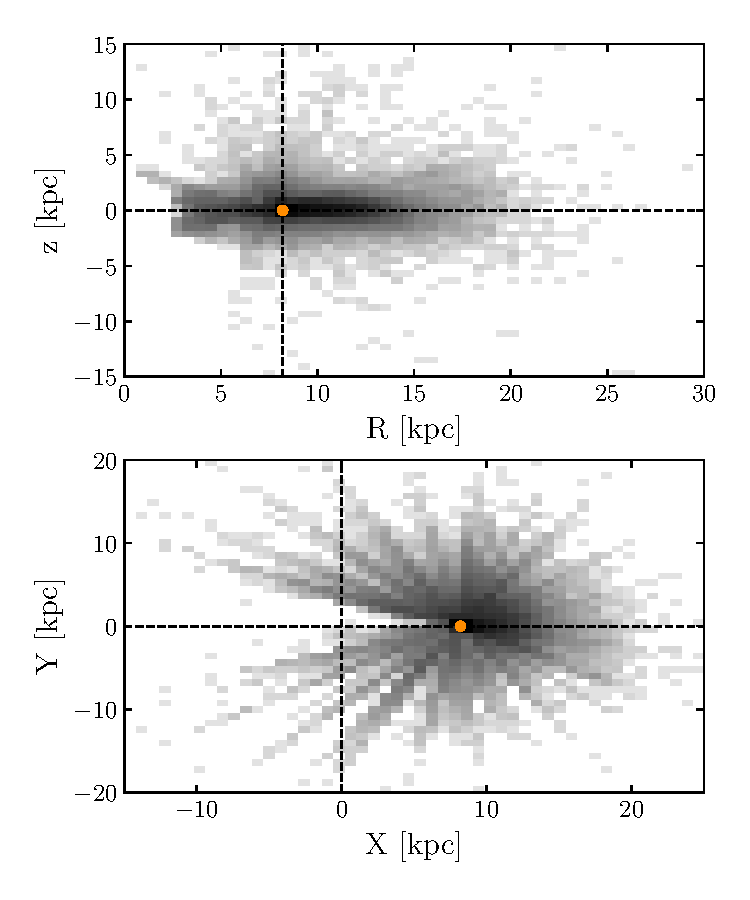
\includegraphics[width=0.6\textwidth]{figure/ch2/APOGEEGalactocentricRzXY.pdf}
	\caption{The APOGEE DR16 sample shown in Galactocentric coordinates. The top panel shows Galactocentric cylindrical radius and height above the disc, the bottom panel shows Galactocentric X and Y, where X is along the Sun-Galactic Centre line, and Y is positive in the direction of Galactic rotation. In both panels the Sun is shown at (X,Y,Z) = (8.178~kpc, 0, 0.028~kpc).}
	\label{ch2:fig:APOGEELocations}
\end{figure}
% \fi

We separate the APOGEE stars into three categories: halo, thin disc, and thick disc using their [Fe/H] and [Mg/Fe] abundances as well as their velocities. We stress that the division into a thin and thick disc is purely an approximation to the more complex structure of the disc, but one that is good enough for our main purpose of investigating the stellar halo. Figure~\ref{ch2:fig:APOGEEAbundances} shows these abundances for our final APOGEE sample, as well as the boundaries we adopt to separate each stellar population. We choose these boundaries based on the number density of APOGEE stars in the abundance space, as well as their eccentricities (which color-codes the points in the top panel of Figure~\ref{ch2:fig:APOGEEAbundances}). The thin-thick disc boundary follows the upper edge of the low-[Mg/Fe] disc locus, while the disc-halo boundary follows the low-[Fe/H] edge of the disc locus and approximately matches the transition from low to high eccentricity. We also add to the halo sample any stars lying in the thin or thick disc chemical regions which have net velocities with respect to their local circular velocity frame which are greater than the magnitude of their local circular velocity: $\lvert \vec{v} - \vec{v}_\mathrm{circ}(R) \rvert > \lvert \vec{v}_\mathrm{circ}(R) \rvert $. We find that this efficiently attributes many higher metallicity stars with genuine halo kinematics to the halo sample. We examine the energy and angular momentum plane, as well as the tangential and radial velocity plane for each of these selections to ensure that they reflect what we expect from the kinematics of the respective populations. Overall, however, the accuracy of this separation is not a major concern, because this only sets the positions based on which velocities will be sampled from the individual DFs. 

The final separated samples consist of 124,879 thin disc stars, 23,543 thick disc stars, and 2,198 halo stars. Like the \solar\ sample, the \survey\ samples consist of six individual sets of orbits which differ by the value of $\beta$ used for the halo DF. Again, the first five samples each use a different value of $\beta$ from among $[0,-0.5,0.5,0.7,0.9]$, while the sixth sample has a composite stellar halo consisting of a 50:50 mixture of orbits from DFs with $\beta=0.5$ and $0.9$ respectively.

\begin{figure}
	\centering
	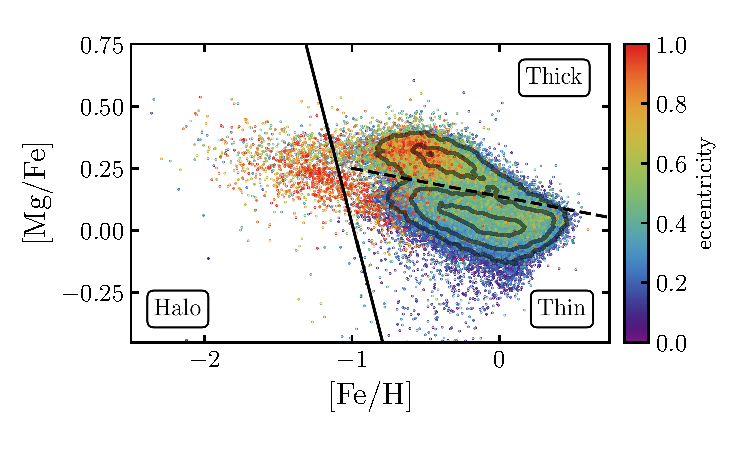
\includegraphics[width=0.75\textwidth]{figure/ch2/APOGEEDR16HaloDiscALPHAFE.pdf}
	\caption{[Mg/Fe] versus [Fe/H] abundances for the APOGEE DR16 sample. Each star is color-coded by its eccentricity, with higher eccentricity stars appearing above lower eccentricity stars. The solid line shows the separation between halo and disc stars. The dashed shows the separation between thin and thick disc stars. The grey contours show density in the more populated thin and thick disc sequences.}
	\label{ch2:fig:APOGEEAbundances}
\end{figure}

To add a degree of realism to the \survey\ samples we perturb all (thin disc, thick disc, and halo) of the velocities using the uncertainties of the \textit{Gaia} and APOGEE DR16 data to which these samples are matched. We do not perturb sample positions, since they are matched to data which are naturally subject to positional uncertainty, and therefore to perturb the positions would be to duplicate the effect. Velocities, on the other hand are drawn from the DFs, and so are not subject to any uncertainties. We first convert the sample velocities into observer coordinates: ($\mu_\mathrm{RA}$, $\mu_\mathrm{Dec}$, $v_\mathrm{los}$), and then add to each of the vectors an amount sampled from a multivariate Gaussian with zero mean and covariance matrix composed of the uncertainties and correlations drawn from the \textit{Gaia} DR2 and APOGEE data. We assert that there are no correlations between APOGEE line-of-sight velocities and any of the \textit{Gaia} data.

\subsection{Sample Kinematics}
\label{ch2:subsec:SampleKinematics}

For both the \solar\ and \survey\ set of samples we calculate kinematic quantities as well as actions using \texttt{galpy} \parencite{bovy15}. Actions are calculated using the ``St\"{a}ckel fudge'' method of \textcite{binney12}. In this approach our Milky Way potential is locally approximated for each individual sample orbit as a St\"{a}ckel potential using a focal length estimated with equation~(9) of \textcite{sanders12}. Eccentricities are similary calculated using a variation of the ``St\"{a}ckel fudge'' method as described in \textcite{mackereth18c}. These actions and eccentricities are calculated in the axisymmetric \texttt{MWPotential2014} potential. 

Potentials like that of the Milky Way are well-represented by St\"{a}ckel potentials \parencite{dejonghe88}, and the `St\"{a}ckel fudge'' approximation gives more accurate action estimates for general orbits when compared with the spherical and adiabatic approximations, which are only good approximations when the potential is close to spherical, and the orbit is confined near the symmetry plane of an axisymmetric potential respectively. As shown by \parencite{bovy15} the variation in St\"{a}ckel method action estimates throughout an orbit is less than about 2~per cent for a disc-like orbit with reasonable radial and vertical extent. \textcite{mackereth18c} find that the St\"{a}ckel approximation performs just as well as direct orbit integration for essentially all halo orbits and most disc-plane orbits which do not venture near the center of the galaxy (where resonances tend to complicate the orbit structure). We test the constancy of this approximation by calculating focal lengths and actions for a few randomly selected APOGEE halo stars at multiple points along their orbits. We find the typical median absolute deviation to be 7~kpc~km~s$^{-1}$ for the radial actions and 3~kpc~km~s$^{-1}$ for the vertical action ($L_{z}$ is obviously invariant along the orbit). The typical median absolute deviations expressed relatively are 2 per cent for the radial actions and 1 per cent for the vertical action, which is similar to the findings of \textcite{bovy15}.

We consider six kinematic spaces which are commonly used throughout the literature for both structure identification and classification, particularly of halo populations. The first two use only velocity information, while the latter four rely on conserved quantities calculated using the underlying potential. For each space we provide a few recent example studies which have made use of it, but the list is by no means exhaustive. The first is the $v_{R}-v_{T}$ plane \parencite[e.g. ][]{belokurov18, fattahi19,lancaster19,mackereth19a,belokurov20, feuillet20}, which is useful since disc and halo populations occupy distinct loci defined by their mean $v_{T}$, and disc populations have much lower tangential and radial velocity dispersions than halo populations. Additionally the degree of radial bias in a halo population is easy to gauge by the radial extent of its velocity ellipsoid. The second space is the Toomre diagram \parencite[e.g. ][]{hawkins15,helmi18,koppelman19b,feuillet20,cordoni20} which plots the quadrature $\sqrt{v_R^2+v_z^2}$ of the $v_{R}$ and $v_{z}$ velocities (also known as $v_\mathrm{perp}$) as a function of $v_{T}$. Here we use cylindrical velocities, yet the Toomre diagram is also often expressed using $UVW$ velocities. In samples that span a large range in Galactic azimuth, the $v_R$ and $v_T$ velocities project onto $U$ and $V$ in a manner that renders the diagram less useful. The advantage of the Toomre diagram is that it factors in $v_{z}$ in addition to $v_{R}$, further isolating halo populations thanks to the relatively cold vertical velocity kinematics of the thin and thick disc populations.

The next three spaces all use angular momentum about the disc rotation axis, $L_{z}$, as the abscissa. $L_{z}$ is an effective coordinate since disc stars tend to have characteristically large, positive values. Additionally, because it is one of three actions, it is conserved under adiabatic conditions. The third space is the $E-L_{z}$ plane \parencite[e.g. ][]{helmi18,koppelman19b, naidu20,feuillet20,cordoni20,horta21a}, which is perhaps the most widely used kinematic space for structure identification in the \textit{Gaia} era. This is due to the relative ease with which these parameters are calculated, their approximate conservation through cosmic time, the fact that the disc occupies a compact locus at high $L_{z}$ and moderate $E$, and that the energy encodes both radius and velocity information. We plot all energies offset by the potential of \texttt{MWPotential2014} at infinity, $\Phi_{0}$, so that $E<0$ are bound orbits. The fourth space is the root of the radial action, $\sqrt{J_{R}}$, as a function of $L_{z}$ \parencite[e.g.][]{trick19,feuillet20,matsuno21,horta21a}. By using the radial action this space can very efficiently separate halo stars on tangential versus radial orbits. This is because the action labels the entire orbit while velocities, for example, will change throughout an orbit. We use the square root of the radial action to compactify the vertical axis for efficient visualization. The fifth space is eccentricity ($e$) as a function of $L_{z}$ \parencite[e.g.][]{cordoni20}. While this specific two-dimensional space is not commonly used, eccentricity as a single parameter is often used as a metric to separate GS/E from the remainder of the stellar halo since it reflects the overall radial extent of an orbit \parencite[e.g.][]{belokurov18,mackereth20,naidu20}.

The final space is the ``action diamond'' \parencite[e.g. ][]{vasiliev19,myeong19,monty20,cordoni20,naidu20} which in our implementation plots $J_{z}-J_{R}$ as a function of $L_{z}$, the azimuthal action. But both quantities are scaled by the total action defined as $J_\mathrm{tot}=\lvert J_{R} \rvert + \lvert J_{z} \rvert + \lvert L_{z} \rvert$, which causes the appearance of a characteristic diamond-shaped boundary (Note that if the normalizing total action is $J_\mathrm{tot}= \sqrt{ J_{R}^{2} + J_{z}^{2} + L_{z}^{2}}$ the boundary is circular, e.g., \textcite{naidu20}). One advantage of this space is that the quantities are scaled by their total action, which means that disc populations whose action budget is dominated by $L_{z}$ tend to cluster tightly in the right corner of the bounding diamond. For the same reason halo sub-populations which arise from, for example a single merger event, are likely to cluster at a single location defined by the actions of the progenitor. The downside of this space is that since all quantities are normalized by the total action, populations which differ by an overall magnitude in their actions, such as eccentric disc and halo populations, may appear indistinct. To combat this effect it is often adviseable to use this space only with a sample confined to a narrow range of radii or $L_{z}$.

It is natural to consider whether higher dimensional spaces would be more appropriate for this type of study. While we have mentioned above many unique quantities that describe stellar orbits, they are not all completely independent. We believe that there are three broad classes of quantities here that we consider here. First are quantities that describe tangential motion, which includes $v_{T}$ and $L_{z}$ (whether it is normalized by $J_\mathrm{tot}$ or not. The second are quantities which describe the magnitude of radial motion, which include $v_{R}$, $v_\mathrm{perp}$, energy, and $J_{R}$. The third are scaled quantities which describe the radiality of an orbit, which include the normalized quantity $(J_{z}-J_{R})/J_\mathrm{tot}$ and eccentricity. Within each of these categories is a modest to large amount of degeneracy. For example a star with high radial velocity likely also has a large $v_\mathrm{perp}$, energy, and $J_{R}$. On the other hand, a star with large radial velocity may not necessarily be on a particularly radial orbit if its tangential velocity is also large. This suggests that the largest dimensional space which would be useful in a coherent sense would be three dimensional. We will explore the possibility of using higher dimensional spaces to select high purity samples of stars from high-$\beta$ populations in \S~\ref{ch2:subsec:SeparatingHighBetaPopulations}. For now we will continue to work with two dimensional spaces for ease of visualization.


Figure~\ref{ch2:fig:SolarKinematics} shows these six kinematics spaces for the \solar\ samples. The disc samples, both thin and thick together, are shown as the black contours, while the halo samples are shown as blue points. Each of the columns shows one of the six different halo models. Figure~\ref{ch2:fig:SurveyKinematics} is the same as Figure~\ref{ch2:fig:SolarKinematics}, but shows the kinematics for the \survey\ samples instead. The disc sample contours are constructed by binning the data with 40 bins across each dimension in each space. The contour levels are then placed at 1, 10, and 100 samples per bin. 

\begin{figure}
	\centering
	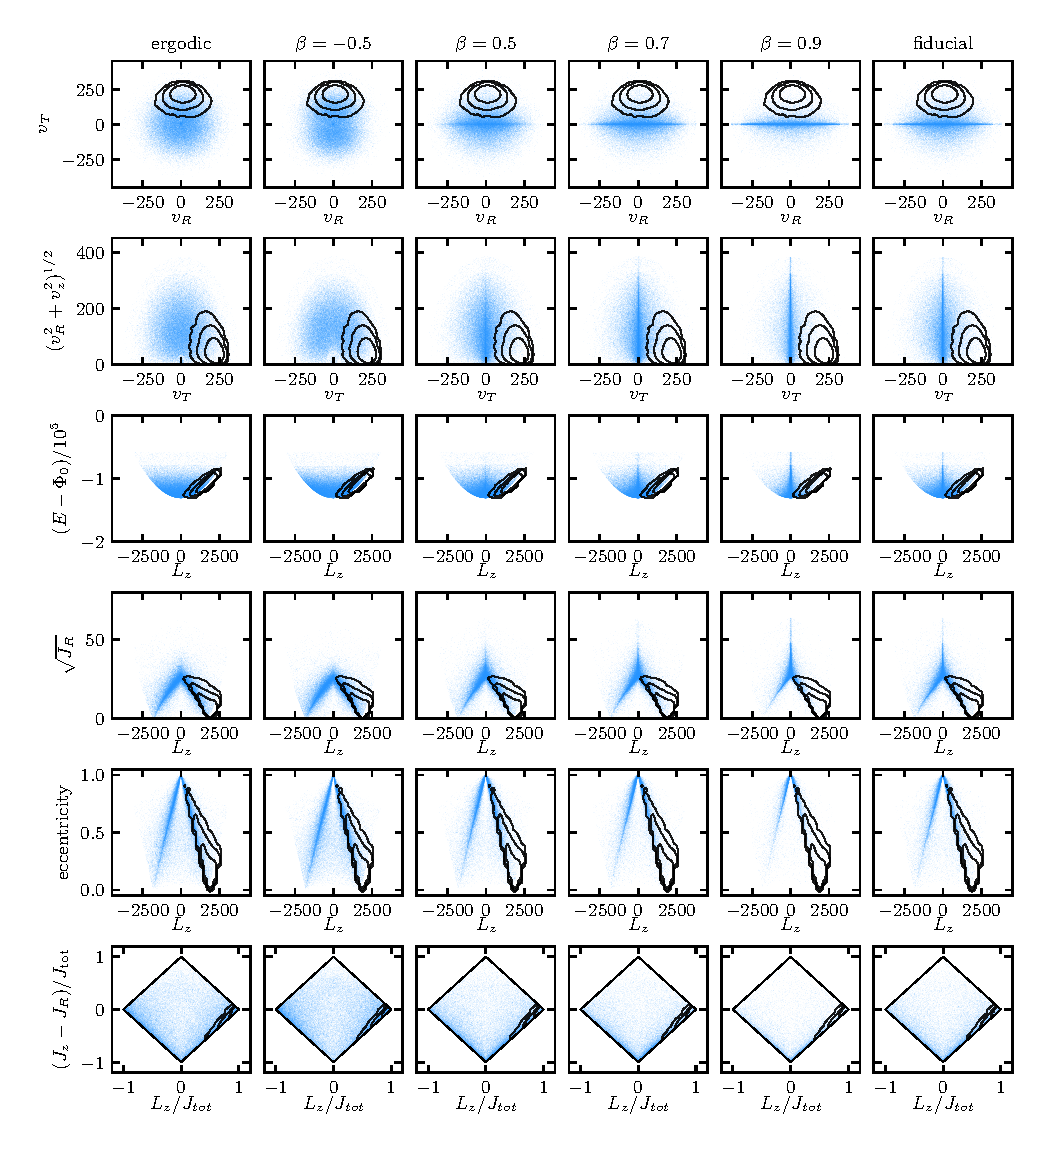
\includegraphics[width=\textwidth]{figure/ch2/SolarKinematicsGrid.pdf}
	\caption{Kinematics of the six \solar\ samples. Each of the columns shows one of the subsets of the \solar\ sample, which vary by the $\beta$ of the halo component (labelled). The blue points show the halo samples while the black contours show the disc samples, combining both thin and thick. \textit{Top row:} Radial and tangential velocities; \textit{second from top:} Toomre diagram; \textit{third from top:} energy and $L_{z}$; \textit{third from bottom:} $\sqrt{J_{R}}$ and $L_{z}$; \textit{second from bottom:} eccentricity and $L_{z}$; \textit{bottom row:} action diamond. The units (unlabelled) are as follows: velocities are in km~s$^{-1}$, actions and angular momenta are in kpc~km~s$^{-1}$, and energies are in km$^{2}$~s$^{-2}$.} \label{ch2:fig:SolarKinematics}
\end{figure}

\begin{figure}
	\centering
	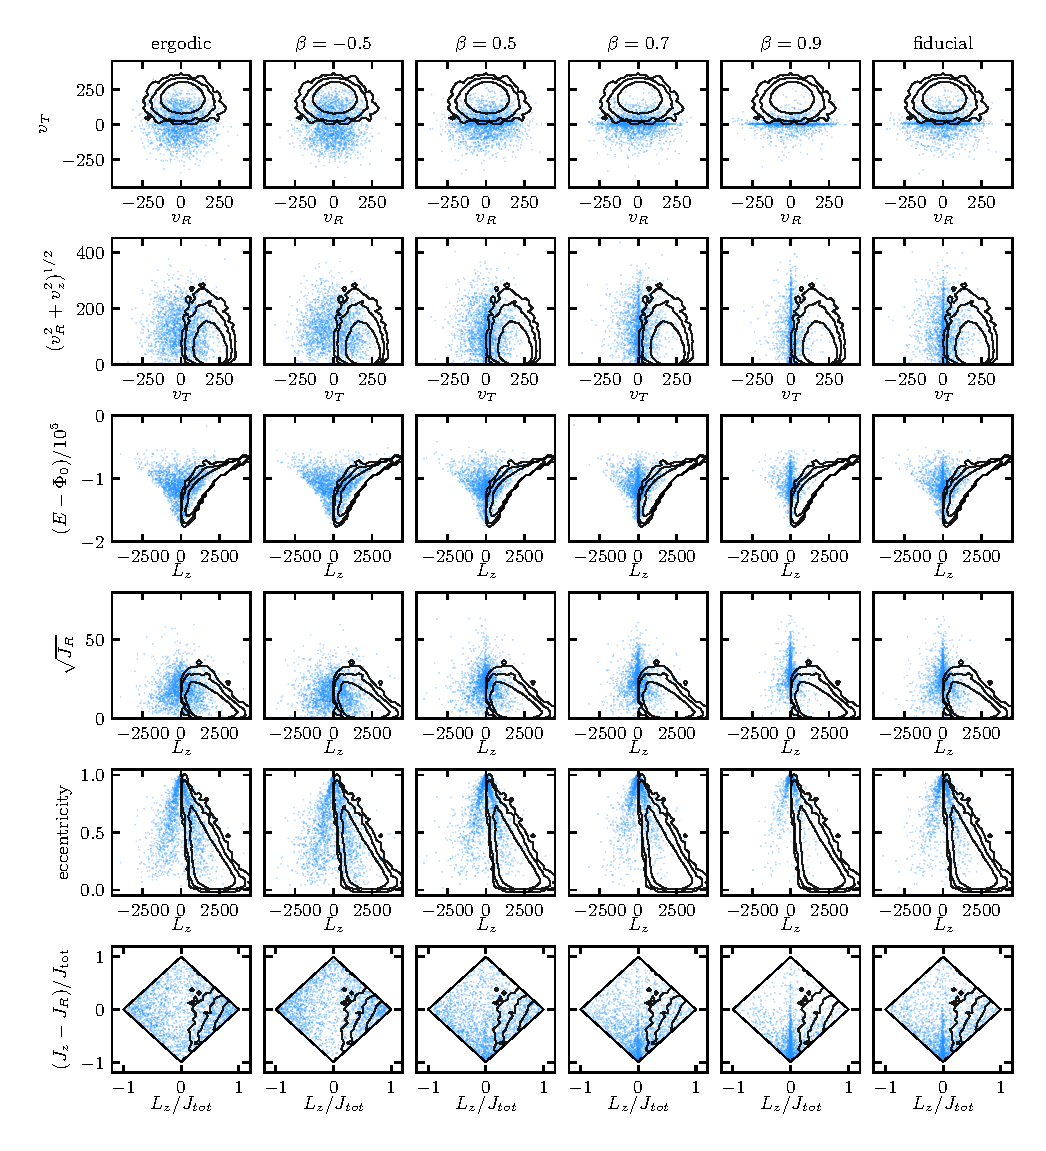
\includegraphics[width=\textwidth]{figure/ch2/SurveyKinematicsGrid.pdf}
	\caption{Same as Figure~\ref{ch2:fig:SolarKinematics} but for the six \survey\ samples.}
	\label{ch2:fig:SurveyKinematics}
\end{figure}

\section{Exploring the Kinematic Properties of our Samples}

In this section, we examine in detail each of the kinematic spaces we presented in the previous section. We first provide a qualitative overview of the kinematic spaces, especially with regards to how kinematics change with variations in the value of $\beta$ of the stellar halo DF. 

\subsection{A Qualitative Assessment of the Kinematic Spaces}

\subsubsection{The Solar Samples}

We first take a closer look at the \solar\ sample kinematics from Figure~\ref{ch2:fig:SolarKinematics}. Starting with the $v_{R}-v_{T}$ velocities, we can immediately see a strong degree of evolution in the morphology of the halo samples as $\beta$ changes. Specifically, as $\beta$ increases the dispersion along the $v_{R}$ axis increases and the dispersion along the $v_{T}$ axis decreases, broadly in accordance with the definition of $\beta$. 

One subtle feature is that as $\beta$ increases the density of samples along the $v_{T}=0$ line forms a broad plateau around $v_{R}=0$, rather than the distinct density peak that can be seen when $\beta=0$ for example. This behaviour is the result of a tendancy towards bimodality in the $v_{R}$ direction for high-$\beta$ samples, since stars are on more radial orbits and therefore preferentially have non-zero radial velocities (with equal preference to positive and negative velocities). Examining the fiducial model highlights why it is important to keep this fact in mind. When low and high-$\beta$ populations are shown together, it may appear to be a superposition of two centrally concentrated ellipsoids, yet in reality the lower-$\beta$ population provides the peak at $(v_{R},v_{T}) = (0,0)$ while the radially biased population tends to more evenly populate the low and high radial velocity region. For much higher $\beta$ or when the density profile allows for apocenters at much larger Galactocentric radii, one will also expect to observe a genuine bimodality in the radial velocity direction, with a distinct lack of stars with zero velocity. 

This is noteworthy when modelling the local stellar halo velocity field using, for example, a Gaussian mixture model. One would expect a two-component model to fit the radially anisotropic halo better than a single component. This assessment is supported by the results of \textcite{belokurov18} and \textcite{fattahi19}, who find that using two Gaussian components for the local halo (i.e. one for the metal poor, more isotropic halo, and one for the radially anisotropic halo) produces best-fits which have systematically negative model residuals near $v_{r}=0$ (note they use spherical polar coordinates), and positive model residuals towards larger radial velocities. This indicates that the single component fit to the radially anisotropic population expects more stars near $v_{r}=0$ and fewer at large radial velocities, in accordance with our expectations. Other studies which have used symmetric, bimodal Gaussians have found good fits to data \parencite{lancaster19,necib19}.

The Toomre diagram shows evolution with increasing $\beta$ in a manner similar to the $v_{R}-v_{T}$ plane. As the radial anisotropy of the halo population increases the distribution elongates along the $v_\mathrm{perp}$ axis, and narrows along the $v_{T}$ axis. The inclusion of $v_{z}$ information in addition to $v_{R}$ in the Toomre diagram does tend to separate the halo samples from the disc samples somewhat more than in the $v_{R}-v_{T}$ plane. But the effect is not as pronounced as might be expected, likely because many disc samples have roughly comparable vertical and radial velocities, and so their extent along the $v_\mathrm{perp}$ axis also increases. In both of these first two kinematic spaces, the disc occupies similar loci at $v_{T} \sim 200$~km~s$^{-1}$ with zero net radial or vertical velocity. It is important to note, however, that even in this population of disc samples located at the solar position there are a marginal yet noticable number belonging to the thick disc with near-0 $v_{T}$. In the Toomre diagram even though the halo samples are more distinct, the maximum perpendicular velocities of the hottest thick disc samples approaches 200~km~s$^{-1}$. 

The $E-L_{z}$ plane in the third row of Figure~\ref{ch2:fig:SolarKinematics} exhibits the now famous central enhancement of samples with $L_{z} \approx 0$ for large $\beta$. It is this feature which is most characteristic of the GS/E population as first shown by \textcite{helmi18}. One of the reasons this space has been studied so frequently in the \textit{Gaia} era is that both $E$ and $L_{z}$ are approximately conserved integrals of motion, and therefore the appearance of stellar (sub)structures in this space often point to a common ancestry for the constituent stars. Another key feature of this space which we will explore in more depth later is the distinct parabolic shape of the overall distribution. This boundary is set by the fact that for a given energy and radius the magnitude of the velocity is fixed. This results in a bounding value of $L_{z}$ which occurs when the velocity is wholly oriented in the direction of $v_{T}$. The equation of the bounding curve is: $E = L_{z}^{2}/(2R^{2}) + \Phi(R)$. Because the samples in the \solar\ set are all at a fixed radius the boundary is obvious in Figure~\ref{ch2:fig:SolarKinematics}. There is also a clear gradient in energy, with the density of samples decreasing as the energy increases. This is intrinsic to the energy-dependence of spherical DFs \parencite[see chapter 4.3 in ][]{binney08} and is therefore observed even at a fixed radius. As the radius changes, the energy of the apex of the bounding parabola also changes. This emphasizes that the relationship between radius and energy is complicated, a feature which we will discuss more later.

The radial action, $J_{R}$, is perhaps the most natural variable for isolating stars from populations with high radial anisotropy, because it labels the entire underlying orbit rather than being sensitive to the phase of the orbit such as velocities are. We see in Figure~\ref{ch2:fig:SolarKinematics} that there is an approximately inverse relationship between the magnitude of $L_{z}$ and the radial action. This occurs because as angular momentum increases at a fixed position, less of the velocity budget is necessarily contained in radial motions. The relationship is not perfect, however, for two reasons. First, this kinematic space does not account for vertical motions, and second there is a range of energies in the \solar\ samples as we have just discussed. As $\beta$ increases a distinct cusp forms around $L_{z}=0$ spanning a range of $\sqrt{J_{R}}$. The fact that this cusp has a distinct minima (around $\sqrt{J_{R}}\approx25$ $\mathrm{kpc}^{1/2}~\mathrm{km}^{1/2}~\mathrm{s}^{-1/2}$ in Figure~\ref{ch2:fig:SolarKinematics}) reflects the fact that at the solar circle, the only orbits that exist with $L_{z}=0$ must either have a certain degree of radial motion, or otherwise must be on a circular orbit exactly over the Galactic pole. The cusp spans a range of $\sqrt{J_{R}}$ for the same reason that the inverse relationship between $\sqrt{J_{R}}$ and $L_{z}$ is imperfect at non-zero $L_{z}$: there is a range of energies in the samples and vertical motions are not accounted for.

The relationship between eccentricity and $L_{z}$ is similar in spirit to the relationship between $\sqrt{J_{R}}$ and $L_{z}$. As $L_{z}$ increases at a fixed location, eccentricity must necessarily decrease because orbits become less radial. This lends a characteristic v-shape to the samples in this space. Unlike $\sqrt{J_{R}}$, eccentricity is a ``scaled'' parameter, it depends only on the relative values of the orbit's pericenter and apocenter. Therefore, we see that disc samples appear less distinct from halo samples than in other kinematic spaces. From an intuitive perspective, a halo star with pericenter at the solar circle could have the same eccentricity as a disc star with apocenter at the solar circle, yet these two stars would have very distinct radial actions. A second curiosity of eccentricity is the fact that as orbits become more radial, their eccentricity approaches 1 asymptotically slowly. This means that as $\beta$ increases samples bunch up close to $L_{z}=0$ and $e=1$. This is markedly different behaviour than most other kinematic spaces we have presented so far, where the kinematic properties of radially-biased samples have a distinct magnitude. Here, the only distinct property of the radially biased population is its sheer density at high eccentricity. We will discuss how this impacts the use of eccentricity as a parameter to select high-$\beta$ populations later.

The action diamond is perhaps the least used among the kinematic spaces shown here, with a similar implementation first being used by \textcite{vasiliev19} \parencite[to our knowledge, although they recognize that the space is analogous to visualisations of three-dimensional action spaces presented by][]{binney08}. Its most common use thus far has been to study globular cluster kinematics and their potential association with larger halo structures \parencite{vasiliev19,myeong19}. But it still offers useful information for the types of aggregate stellar populations we study here. Understanding the action diamond is intuitive. The right and left points of the diamond ($\lvert L_{z} \rvert =J_\mathrm{tot}$) are in-plane prograde and in-plane retrograde orbits respectively. The top point ($J_{z}=J_\mathrm{tot}$) is a polar orbit, and the bottom point ($J_{R}=J_\mathrm{tot}$) is a radial orbit. The bottom-right and bottom-left edges ($J_\mathrm{tot}$ wholly contained in $L_{z}$ and $J_{R}$) are prograde and retrograde in-plane orbits. The top-right and top-left edges ($J_\mathrm{tot}$ wholly contained in $L_{z}$ and $J_{z}$) are prograde and retrograde out-of-plane orbits.

One of the most noticeable features of the action diamond is that both disc and halo populations tend to be biased towards the bottom half of the diamond, which reflects the fact that both populations tend to have modestly hotter radial versus vertical kinematics. Indeed, we see what is perhaps the most subtle transformation in morphology from the low to high-$\beta$ halo population, where the samples appear to concentrate more towards the bottom point of the diamond rather than the left and right points. This results from the dominance of the radial action over the vertical action in the high-$\beta$ sample. The disc also hugs the bottom-right edge of the diamond, but the action budget is dominated by $L_{z}$, meaning it is mainly confined to the right point of the diamond. Similarly to eccentricity this is also a ``scaled'' space, so two orbits with different absolute kinematic properties may occupy the same point. So, while the strength of the action diamond lies in the fact that distinct types of orbits occupy different loci in the space, the weakness is that confusion between two populations that may have different absolute kinematics, but similar types of orbits is likely. This will become more evident when examining the \survey\ sample set.

\subsubsection{The \textit{Survey} Samples}

The \survey\ samples differ from the \solar\ samples in three key respects with regards to the six kinematic spaces that we consider. First, the sample positions span a range of Galactocentric radii, and so in some sense it is useful to consider the kinematic profiles as a superposition of many of the individual samples seen in Figure~\ref{ch2:fig:SolarKinematics}, but determined at different radii. Second, the samples are perturbed by \textit{Gaia} and APOGEE errors. Third, and perhaps most important, is that the positions underlying the samples are subject to the complicated APOGEE DR16 selection function. It is through these three lenses that we will assess the kinematics of the \survey\ sample set in Figure~\ref{ch2:fig:SurveyKinematics}.

First, one obvious change to all of the kinematic spaces is the increased range over which the disc populations are observed, while in the \solar\ samples the disc populations tended to be confined to a narrow region. This is due mostly to the first two factors mentioned above: the increased radial range over which the DFs are sampled and the addition of realistic uncertainties. Furthermore the discrepancy in the number of disc samples versus halo samples (roughly 66:1) exacerbates the degree to which the disc populations extend into the stellar halo kinematic space with meaningful density.

In the $v_{R}-v_{T}$ plane, the overall morphology of the halo samples stays the same, with bimodality along the $v_{R}$ axis increasing as $\beta$ increases. The impact of the realism steps on the data is clear, particularly in how the \survey\ samples do not cluster so tightly on the $v_{T}=0$ line, especially in the samples with higher $\beta$, as the \solar\ samples do. Overall our fiducial model looks realistic in its representation of the nearby Milky Way $v_{R}-v_{T}$ plane \parencite[c.f. figures 2 and 1 in ][ respectively, although note they use spherical coordinates]{belokurov18,fattahi19}, a testament both to the validity of our models and the steps we take to add realism to our DF samples. The Toomre diagram changes in much the same way as the $v_{R}-v_{T}$ plane: the overall morphology is the same, but the addition of uncertainties has softened the cusp in the halo samples along the $v_{T}=0$ line. In both these planes, the disc population now extends down to near $v_{T}=0$, which reflects the addition of samples from the inner galaxy where the angular momentum is lower and the radial velocity dispersion is higher. The extent of the disc in the $v_{R}$ and $v_\mathrm{perp}$ dimensions does not increase as drastically, because only the increased radial and vertical velocity dispersions in the inner Galaxy serve to modify its extent.

From a qualitative standpoint, the $E-L_{z}$ plane changes in much the same way as the velocity planes. The cuspy overdensity of the high-$\beta$ populations is softened, and the hottest thick disc stars begin to impinge on this characteristic region, yet leave a discernable overdensity of halo samples visible just beyond their boundary. The $E-L_{z}$ plane also shows a distinct change in morphology of the bounding region of the kinematic space, which we mentioned in the previous section is due to there being a fixed velocity budget at a given energy and radius. For the \survey\ sample, where stars at many radii are included, the bounding region is a superposition of many of the aforementioned parabolic curves. These bounding regions tend to get wider as radius increases since the potential scales inversely with distance from the Galactic center. For inner Galaxy samples the bounding parabola is narrow with minima at very negative energies. Conversely, for outer Galaxy stars, the bounding parabola is wide with a minima at higher energy. The superposition of these bounding curves results therefore in a funnel shape which narrows as the energy is decreased. An example of this morphology is shown in Figure~\ref{ch2:fig:ELzBoundaries} where the in-plane bounding parabolas for \texttt{MWPotential2014} corresponding to radii 2-15~kpc are shown.

\begin{figure}
    \centering
    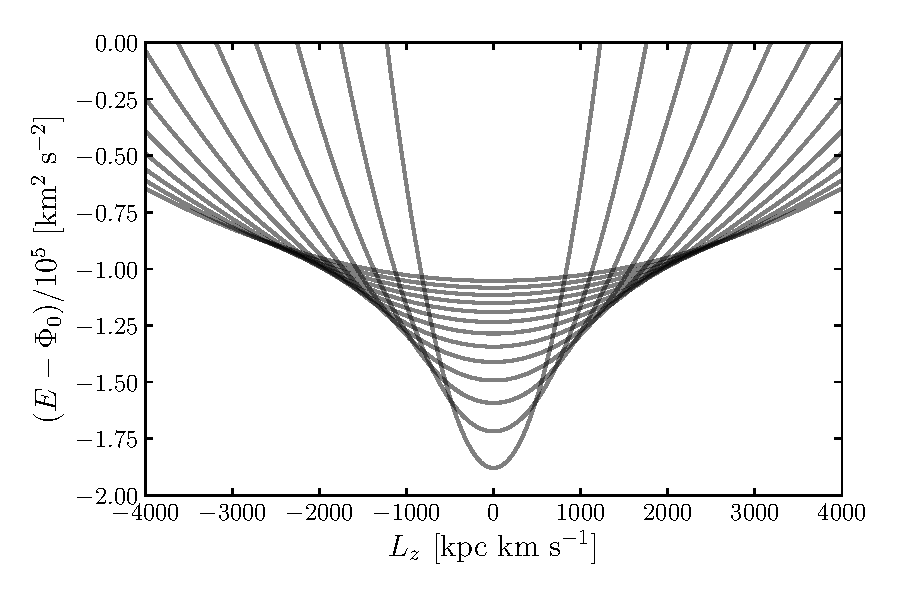
\includegraphics[width=0.75\textwidth]{figure/ch2/ELzBoundingParabolas.pdf}
    \caption{The $E-L_{z}$ plane shown with bounding parabolas corresponding to Galactocentric radii 2 (lowest curve) to 15 (highest curve) kpc. The curves are calculated in-plane ($z=0$), in \texttt{MWPotential2014}.}
    \label{ch2:fig:ELzBoundaries}
\end{figure}

A particularly interesting feature of the \survey\ sample $E-L_{z}$ plane is that there appears to be a region of maximal density which begins at $E \sim -1.3\times10^{5}$ km$^{2}$ s$^{-2}$ and follows an approximate parabolic shape towards larger energies as $\lvert L_{z} \rvert$ increases. These are most obvious in the $\beta=0$ and $0.5$ models, but are also noticable at higher $\beta$. Below this energy there are halo samples, yet they are observed in much lower numbers than at this overdensity. The interpretation of this overdensity is that the majority of the samples in the \survey\ set lie near the Sun, and therefore they tend to be roughly confined by the bounding parabola defined at that location. The occurence of over- and underdensities in $E-L_{z}$ space depending on the underlying radial distribution of samples is something we will explore in the next subsection.

The $\sqrt{J_{R}}-L_{z}$ plane no longer has any indications of the inverse relationship between $J_{R}$ and $L_{z}$ observed in the \solar\ samples and discussed above. Likely the combination of the radial range as well as realistic uncertainties causes all traces of the relationship to disappear. Instead now the halo samples manifest as a broad cloud that is slightly biased either towards $L_{z}$ or $\sqrt{J_{R}}$ depending on the value of $\beta$. The halo samples of the most radially biased models still do exhibit a diffuse cusp along the $L_{z}$ = 0 line. The differences in the $e-L_{z}$ plane tell a similar story. There is no longer as sharp an inverse relationship between eccentricity and $L_{z}$ as was observed in the \solar\ samples, yet the relationship is at least somewhat apparent in contrast with the $\sqrt{J_{R}}-L_{z}$ plane. The higher $\beta$ models still tend to simply cluster more tightly around $L_{z}=0$ and $e=1$, similar to the \solar\ samples. Notably, the disc samples extend all the way to the high-$\beta$ overdensity, and in general completely dominate the prograde half of the plane.

In the action diamond, the disc populations transition from occupying a narrow strip near the prograde corner to dominating the lower right quadrant of the diamond. This large change in area of the disc populations demonstrates a weakness in the action diamond (indeed one shared by eccentricity), which is that ``scaled'' kinematic quantities often confuse orbits that only broadly share certain properties. In this case, when the vertical and radial actions of the hottest thick disc stars become of order comparable with their $L_{z}$ they migrate towards the center and bottom corner of the diamond overlapping with the halo samples, even though the magnitude of their actions can be quite different from those of stars in the halo. The halo samples have the same qualitative trends as are seen in the \solar\ samples. As $\beta$ increases, the samples concentrate near the bottom of the figure. Additionally of note is that very few ergodic samples occupy this region of the diagram, they are more uniformly spread throughout the space and even biased towards the high-$L_{z}$ corners. This means the bottom corner is likely a good region to isolate radially biased halo populations from ergodic populations.

\subsection{The Impact of the Underlying Radial Distribution of Samples on the \texorpdfstring{$E-L_{z}$}{E-Lz} plane}
\label{ch2:subsec:RadialBiases}

In the previous section, we noted that the \survey\ samples exhibit an interesting change in morphology in the $E-L_{z}$ plane when compared with the \solar\ samples. In the $E-L_{z}$ plane of the latter (Figure~\ref{ch2:fig:SolarKinematics}) the samples were confined by a bounding parabola defined by the escape velocity as a function of changing energy at a fixed Galactocentric radius (this being the location of the Sun in the \solar\ sample). Sample density decreases as energy increases moving away from the bounding parabola. The radially biased samples have a higher energy cusp around $L_{z}=0$, leading to different overall morphology but the same trend still holds. This phenomenon lead us to interpret the apparent overdensity in the $E-L_{z}$ plane of the low-$\beta$ \survey\ samples around $E \sim -1.3\times10^{5}$ km$^{2}$ s$^{-2}$ as being caused by the concentration of the samples near the Sun.

While this observation is not particularly unexpected, it suggests a question: what would happen if the intrinsic radial distribution of samples (i.e. the APOGEE DR16 data which sets the approximate positions of our samples) took a more complicated form? We can investigate this using APOGEE DR16 by augmenting the \survey\ sample with additional samples directed towards the Galactic bulge. Recall that we do not consider any stars for inclusion in the \survey\ sample if they have $-20\degr < \ell < 20\degr$ and $|b| < 20\degr$. Here, just to investigate the radial distribution of samples, we soften that requirement and allow stars lying in this angular range with Galactocentric radius greater than 3~kpc to be included into the \survey\ sample set. Note that this distance from the Galactic center is approximately equal to the distance from the Galactic center enforced by the $20\degr$ angular cut we use to define the \survey\ sample - i.e. $\tan(20\degr) \times 8.178~\mathrm{kpc} \approx 3~\mathrm{kpc}$. This radius is also the radius at which the density of the bulge component of \texttt{MWPotential2014} drops below the density of our stellar halo model when it is normalized to have the mass found by \textcite{mackereth20}. This is all to say that we are confident we do not introduce many bulge stars into the sample by including these new data. Separating halo stars from disc stars, sampling kinematics from the DF, and the perturbation by uncertainties are all done in the same manner as described in \S~\ref{ch2:sec:DFSamples}. This results in 497 new halo samples.

The top panel of Figure~\ref{ch2:fig:APOGEERadialBias} shows the radial distribution of the \survey\ samples, the additional samples in the direction of the Galactic center, and their combination. Note that a number of the additional Galactic center samples appear at radii less than 3~kpc. This can be attributed to the perturbation by the APOGEE and \textit{Gaia} uncertainties. The overall distribution of radii is clearly bimodal, with peaks around 3.5 and 8~kpc, and a decrease at 6~kpc. The inner peak is driven mostly by the additional samples from the inner Galaxy pointings, but hints of the overdensity are clearly present in the \survey\ sample. The occurence of this bimodality is undoubtedly caused by the APOGEE selection function, and specifically the location of the survey pointings.

\begin{figure}
    \centering
    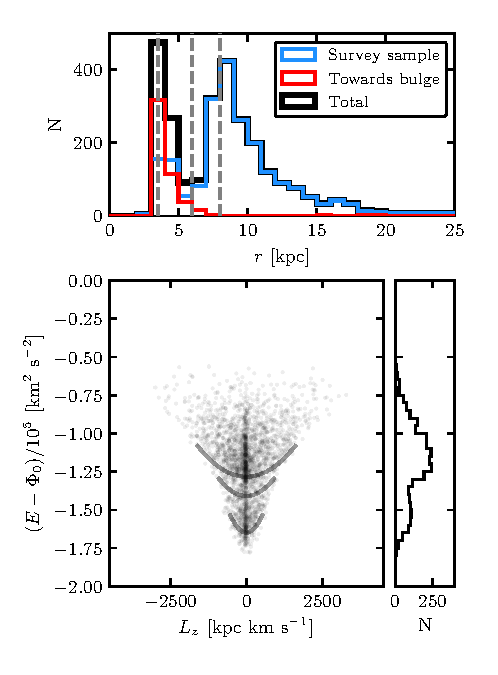
\includegraphics[width=0.75\textwidth]{figure/ch2/APOGEEHaloRadialBias.pdf}
    \caption{\textit{Top:} Histogram of Galactocentric radii for the \survey\ sample (blue), the additional samples towards the Galactic bulge (red), and their combination (black). \textit{Bottom left:} $E-L_{z}$ plane for \survey\ sample augmented by the additional sources towards the Galactic bulge. \textit{Bottom right:} Histogram of energies for the same sample. Three grey dashed lines in the top panel mark the locations of over and underdensities in the radial distribution at 3.5, 6, and 8 kpc. Three black lines in the bottom panel show sections of the bounding parabolas for those corresponding radii, roughly marking the boundaries between over and underdensities in the $E-L_{z}$ plane.}
    \label{ch2:fig:APOGEERadialBias}
\end{figure}

The bottom-left panel of Figure~\ref{ch2:fig:APOGEERadialBias} shows the $E-L_{z}$ plane for the fiducial model of the \survey\ sample plus the additional samples towards the Galactic center, 2,695 samples in total (halo samples only, no disc). It is immediately clear that there is an underdensity between $-1.25$ and $-1.5\times10^{5}$~km$^{2}$~s$^{-2}$. This is confirmed by examining the bottom right panel, a histogram of energies, which highlights the overdensity at the aforementioned location. It does not perfectly highlight the overdensity because, as we have established, the density fluctuations occur on roughly parabolic contours, but nontheless its signature is there. Overlaid on the figure are three black lines that are sections of the bounding parabolas corresponding to the three radii marked with grey dashed lines in the top panel: 3.5, 6, and 8~kpc. The bottom and top curves (3.5 and 8~kpc) cradle the two overdensities, while the middle curve at 6~kpc cradles the underdensity. This clearly illustrates that the uneven radial distribution of samples is clearly linked to the appearance of substructure in the $E-L_{z}$ plane.

\section{The Purity of Populations of Interest}
\label{ch2:sec:PurityOfPopulations}

One of the most useful questions we might ask is whether we can use our samples to identify which kinematic spaces are best for identifying certain populations that we are interested in separating from a background of contaminants. For the purposes of this work we focus on separating the high-$\beta$ populations from low-$\beta$ and disc populations.

\subsection{Separating High-\texorpdfstring{$\beta$}{beta} Populations from Low-\texorpdfstring{$\beta$}{beta} and Disc Populations}
\label{ch2:subsec:SeparatingHighBetaPopulations}

The separation of high-$\beta$ populations from low-$\beta$ populations is currently of special importance, because the two dominant inner-Milky Way halo populations are the \textit{in-situ} low-$\beta$ component and the high-$\beta$ GS/E component \parencite{belokurov18,helmi18,iorio21}. While these two populations do have somewhat unique chemistry \parencite{haywood18}, it is not so distinct that that abundances are an efficient means of separating them, such as is the case for separating the disc populations both from one another and from the halo. Building on this sentiment, we do not even know \textit{a priori} the detailed chemical profile of the \textit{in-situ} and GS/E components so that we might try and separate them using their abundances. Their individual chemistries can only be effectively learned if the populations can be separated by some other means. Additionally, detailed mass modelling in the halo requires some means of tagging different populations of interest. For example \textcite{mackereth20} divide the halo into mono-abundance populations. They use a simple eccentricity cut to separate ergodic and high-$\beta$ populations. Here we will delve deeper into the methods for kinematically separating these two major halo populations.

While in the previous section, our focus was on faithfully reproducing the types of samples observed in modern datasets, here we must focus on numerical accuracy. We therefore increase the number of samples in the \survey\ sample set so that the small number of halo stars used to generate the model (2,198) does not impact the fidelity of our results. We do this by generating one hundred different velocity samples at each APOGEE halo star location, rather than just one, for each halo DF with a different $\beta$. This ``augmented'' \survey\ sample set is otherwise processed exactly the same as described in \S~\ref{ch2:subsec:TheSurveySamples} and \ref{ch2:subsec:SampleKinematics}. For the disc we increase the number of samples by a factor of ten in the same manner. We use these augmented \survey\ samples for the remainder of the paper, and the \solar\ samples remain unchanged.

We use our fiducial halo model to investigate the purity of ergodic and high-$\beta$ populations; recall that the fiducial halo model consists of a 50:50 mixture of $\beta=0.5$ and 0.9 populations. Figures~\ref{ch2:fig:SolarHaloPurity} and \ref{ch2:fig:SurveyHaloPurity} show the purity of the high-$\beta$ component of the fiducial model with respect to the low-$\beta$ component for the \solar\ and \survey\ sample sets respectively. Purity is calculated as $N_\mathrm{\beta=0.9}/(N_\mathrm{\beta=0.9}+N_\mathrm{\beta=0.5})$, and the data is binned with 40 bins across each dimension of each kinematic space. Overlaid on each kinematic space is the lowest contour of the disc samples from Figures~\ref{ch2:fig:SolarKinematics} and \ref{ch2:fig:SurveyKinematics} to indicate where the disc may contribute contaminants to the purity measurement.

\begin{figure}
	\centering
	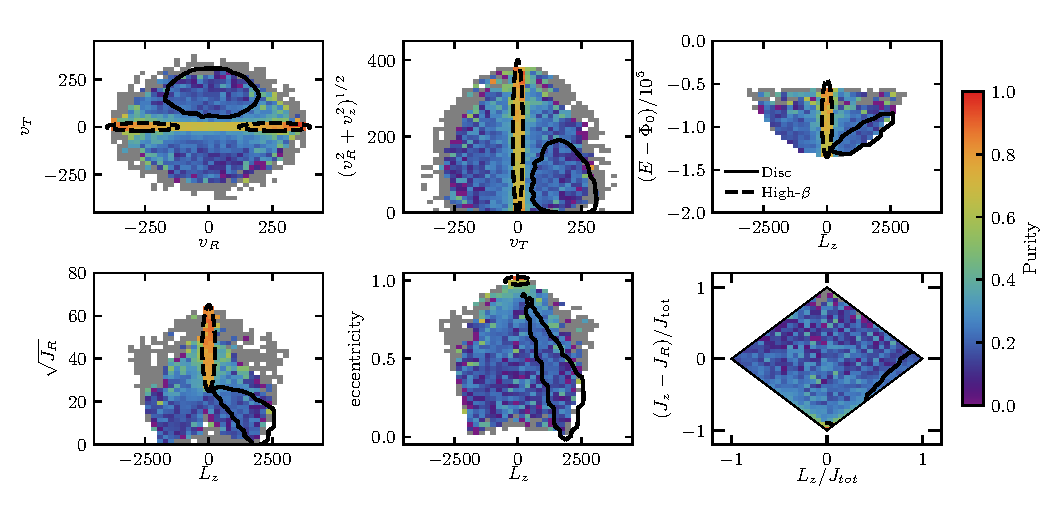
\includegraphics[width=\textwidth]{figure/ch2/SolarHaloPurityGrid.pdf}
	\caption{Purity of high-$\beta$ halo samples with respect to low-$\beta$ samples for the \solar\ sample set. The kinematic spaces and units are as described in Figure~\ref{ch2:fig:SolarKinematics}. The grey bins are those with fewer than 5 samples in them. In each of the panels the dashed black ellipse(s) show the selection ellipses for the high-$\beta$ sample. The solid black contour is the lowest contour of disc stars from Figure~\ref{ch2:fig:SolarKinematics}.}
	\label{ch2:fig:SolarHaloPurity}
\end{figure}

\begin{figure}
	\centering
	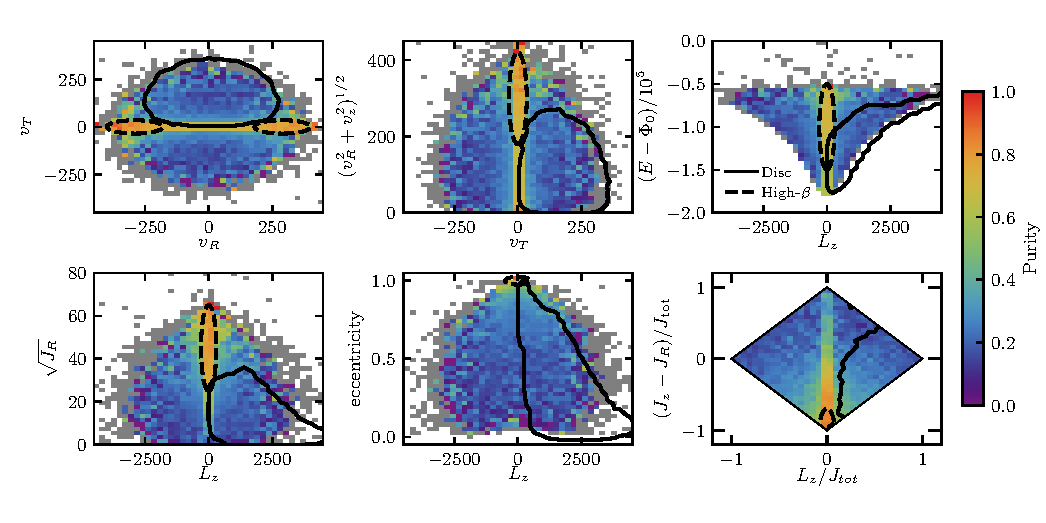
\includegraphics[width=\textwidth]{figure/ch2/SurveyHaloPurityGrid.pdf}
	\caption{Same as Figure~\ref{ch2:fig:SolarHaloPurity} but for the augmented \survey\ sample set. Here, the solid black contour shows ten samples per bin calculated in the same manner as Figure~\ref{ch2:fig:SurveyKinematics}.}
	\label{ch2:fig:SurveyHaloPurity}
\end{figure}

Qualitatively, the purity of high-$\beta$ samples follows intuitively from Figures~\ref{ch2:fig:SolarKinematics} and \ref{ch2:fig:SurveyKinematics}. In the $v_{R}-v_{T}$ and Toomre diagrams the purity is highest along the $v_{T}=0$ axis and at large values of $v_{R}$ and the $v_\mathrm{perp}$ respectively. In the $E-L_{z}$ plane, we see that the purity is highest when $L_{z}$ is zero and at modest to high energies. The $\sqrt{J_{R}}-L_{z}$ plane behaves similarly, with a cloud of high-purity at large values of the radial action near $L_{z}=0$. Eccentricity is peculiar, as we have already noted in that being a ``scaled'' parameter the radially biased populations do not occupy a distinct region of the space. Rather they tend to cluster with greater density near $L_{z}=0$ and $e=1$. This behaviour is necessary to keep in mind when evaluating this space on the merits of high-$\beta$, because one might assume that the best place to isolate radially biased populations is near $e=1$ but at higher $L_{z}$. In reality, the bulk of the sample lies at $L_{z}=0$ but simply exists at lower purity because the ergodic sample also populates that region. The action diamond exhibits the highest purity at the bottom corner where the radial action dominates the action budget. In particular in the \solar\ sample, the region of high-purity is only seen in the few pixels around the apex of the diamond.

\begin{table}
    \centering
    \caption{High-$\beta$ selection ellipse parameters for the \solar\ and \survey\ samples in six kinematic spaces. Ellipses correspond to those in Figures~\ref{ch2:fig:SolarHaloPurity} and \ref{ch2:fig:SurveyHaloPurity}. See the caption of Figure~\ref{ch2:fig:SolarKinematics} for unit conventions. From left to right the columns are: kinematic space, ellipse center point, ellipse semi-major axes, high-$\beta$ completeness, high-$\beta$ purity for halo samples only, and high-$\beta$ purity including disc samples. Note that here, and throughout the paper, we account for the fact that we augmented the \survey\ halo sample by a factor of 100, while we only augmented the disc sample by a factor of 10 when calculating purity including disc samples as contaminants.}
    \begin{tabular}{cccccc}
         Space & Center [x,y] & SMA [x,y] & C & P$_\mathrm{halo}$ & P$_\mathrm{disc}$ \\
        \hline
        \hline
        \multicolumn{5}{c}{\solar\ sample} \\
        \hline
        $v_{R}-v_{T}$        & $[\pm 260,0]$ & [140,20]    & 0.29 & 0.79 & - \\
        Toomre               & $[0,200]$     & [20,200]    & 0.72 & 0.74 & - \\
        $E-L_{z}$            & $[0,-0.9]$    & [200,0.45]  & 0.72 & 0.74 & - \\
        $\sqrt{J_{R}}-L_{z}$ & $[0,45]$      & [250,20]    & 0.69 & 0.78 & - \\
        $e-L_{z}$            & $[0,1]$       & [500,0.025] & 0.62 & 0.83 & - \\
        Action Diamond       & $[0,-1]$      & [0.1,0.1]   & 0.62 & 0.85 & - \\
        \hline
        \multicolumn{5}{c}{\survey\ sample} \\
        \hline
        $v_{R}-v_{T}$        & $[\pm 290,0]$ & [110,35]    & 0.12 & 0.76 & 0.76 \\
        Toomre               & $[0,300]$     & [35,120]    & 0.15 & 0.71 & 0.70 \\
        $E-L_{z}$            & $[0,-1]$      & [300,0.5]   & 0.74 & 0.66 & 0.62 \\
        $\sqrt{J_{R}}-L_{z}$ & $[0,45]$      & [300,20]    & 0.52 & 0.76 & 0.76 \\
        $e-L_{z}$            & $[0,1]$       & [500,0.025] & 0.61 & 0.82 & 0.82 \\
        Action Diamond       & $[0,-1]$      & [0.08,0.3]  & 0.39 & 0.86 & 0.85 \\
        \hline
    \end{tabular}
    \label{ch2:tab:HighBetaSelections}
\end{table}

When evaluating how each kinematic space performs in separating populations, it is important to keep in mind the overall density of halo stars. Many regions of each space exhibit spuriously high purity where there are only a few halo samples. We therefore consider only bins with greater than 5 samples in them, and render those bins with fewer than 5 samples grey in Figures~\ref{ch2:fig:SolarHaloPurity} and \ref{ch2:fig:SurveyHaloPurity}. With this in mind, we have selected elliptical regions in each space where both the purity is large and the density of high-$\beta$ halo samples is reasonable. These are shown as the dashed black lines in Figures~\ref{ch2:fig:SolarHaloPurity} and \ref{ch2:fig:SurveyHaloPurity}. The parameters of the selection ellipses are given in Table~\ref{ch2:tab:HighBetaSelections}. We choose these simple shapes to represent the high-$\beta$ regions because one goal in this analysis is to emphasize applicability to real data. Shapes which are too specific to the populations here may provide errant results when applied to other data where the kinematic properties may be subtly different (e.g., if either the spatial selection or the potential used to derive kinematics changes). Instead, we pick regions which would be mostly insulated from the peculiarities of a specific data set. In each of the six kinematic spaces at least one of the dimensions probes the circularity of the orbit in the disc plane. Following this, each of the selection regions primarily picks out samples with $L_{z}$ or $v_{T}$ approximately equal to zero (the bottom corner of the action diamond necessarily has $L_{z}=0$). The selections then pick out extreme values of the other quantity, which generally trends with the degree of radial bias in a population (specifically $v_{R}$, $v_\mathrm{perp}$, $E$, and $\sqrt{J_{R}}$). The selection regions of the ``scaled'' spaces tend to be concentrated at the extrema of the scaled quantity (eccentricity and $(J_{z}-J_{R})/J_\mathrm{tot}$). The reason for mentioning the overall trends in our choice of selection regions is that these broad properties should suffice to pick out radially biased samples in any data set, not just specifically our DF models. This is important if, for example, we are to be able to confidently apply these selections to real APOGEE DR16 data, something we plan to do in the near future. 

It is still interesting to ask, however, what is the tradeoff between increasing or decreasing the size of the selection ellipses? Intuitively, a larger selection boundary would include more high-$\beta$ samples, but would also include more low-$\beta$ samples which would decrease purity. To explore this, we make purity-completeness relations for each of the kinematic spaces for both the \solar\ and \survey\ sample sets. To do this we consider two sets of scaling factors: $(x_{1},x_{2})$ where each factor takes the form $x_{i} = 2^{y}$. For each of the two scaling factors we consider 25 values of $y$ uniformly spaced on the interval $[-2,2]$, giving a grid of 625 total combinations. For each of these 625 unique pairs of factors we multiply them to the semi-major axes in Table~\ref{ch2:tab:HighBetaSelections} to generate a new selection ellipse. We then calculate the high-$\beta$ purity and completeness according to this new selection ellipse. To generate an average purity-completeness relationship we bin the 625 purity measurements in completeness and calculate the mean purity in each bin. The results are shown for the \solar\ and \survey\ sample sets in Figures~\ref{ch2:fig:SolarCPDiagram} and \ref{ch2:fig:SurveyCPDiagram} respectively. Each of the panels highlights one kinematic space (labelled), the curves for the other kinematic spaces are shown faintly behind to emphasize differences. In the panels of Figure~\ref{ch2:fig:SurveyCPDiagram} there is a solid and dashed line that show the purity calculated only considering halo samples (solid) and the purity calculated including both halo and disc samples (dashed). Additionally, in each panel there is a colored circled which shows the purity and completeness of the default boundaries shown in Figures~\ref{ch2:fig:SolarHaloPurity} and \ref{ch2:fig:SurveyHaloPurity}.

\begin{figure}
    \centering
    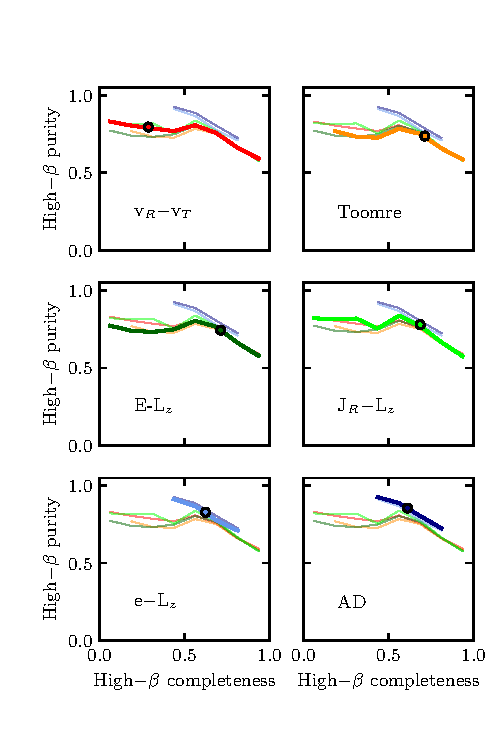
\includegraphics[width=0.7\textwidth]{figure/ch2/SolarHaloCompletenessPurity.pdf}
    \caption{Purity-completeness relation for the fiducial \solar\ sample for each kinematic space (labelled). The bold line in each panel shows the purity calculated only considering halo samples, the solid lines from all other panels are shown faintly in the for context. The filled circle in each panel shows the purity and completeness of the default selections from Figure~\ref{ch2:fig:SolarHaloPurity}.}
    \label{ch2:fig:SolarCPDiagram}
\end{figure}

\begin{figure}
    \centering
    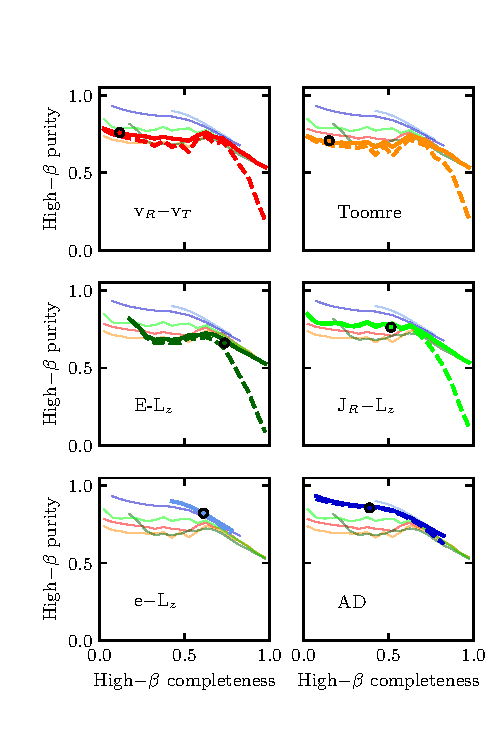
\includegraphics[width=0.7\textwidth]{figure/ch2/SurveyHaloCompletenessPurity.pdf}
    \caption{Same as Figure~\ref{ch2:fig:SolarCPDiagram} but for the fiducial \survey\ sample. Additionally, the bold dashed line in each panel shows the purity calculated including disc samples. Also see Figure~\ref{ch2:fig:SurveyHaloPurity}.}
    \label{ch2:fig:SurveyCPDiagram}
\end{figure}

For the \solar\ samples, the purity-completeness relations are similar for quantities which are similar to one another. $v_{R}-v_{T}$ and the Toomre diagram are similar, $E-L_{z}$ and $\sqrt{J_{R}}-L_{z}$ are similar, and $e-L_{z}$ and the action diamond are similar. The action diamond appears to be the superior space, achieving a higher purity at a given completeness than any other kinematic space. At large completeness the other kinematic spaces are more-or-less tied with one another. The apparant bimodalities (i.e. the peaks near completeness of 0.6) in the purity-completeness relations for the absolute kinematic spaces is just an artifact of how we have visualized the results of this analysis. In general, the linear trend at higher completeness in these spaces captures the variation in the rotation-sensitive quantity ($v_{T}$ and $L_{z}$) when the anisotropy-sensitive quantity ($v_{R}$, $v_\mathrm{perp}$, $E$, and $\sqrt{J_{R}}$ is scaled to a large range. At lower completeness the same trend holds when the radial quantity is scaled to small values. These two trends emerge because of the logarithmic manner in which we generate the scaling factors. A general trend for these four spaces is as follows: at a given ellipse size for the anisotropy-sensitive quantity, a narrower selection for the rotation-sensitive quantity produces higher purity and lower completeness. For the action diamond and $e-L_{z}$ the relations are simple because the high-$\beta$ samples occupy a single locus in these spaces. In general the only takeaway from this analysis applied to the \solar\ samples is that the action diamond appears to outperform the other spaces. We are wary of making any other statements because the simplicity of our \solar\ samples clearly incites slightly pathological results in this specific analysis. 

For the \survey\ samples the differences between the kinematic spaces are more interesting. The action diamond and $e-L_{z}$ plane have very similar purity-completeness relations, with the action diamond having lower completeness and higher purity, and the $e-L_{z}$ plane having higher completeness and lower purity. Both of these spaces have little contamination from disc samples (solid and dashed lines are similar). These two scaled spaces appear superior to the other four spaces under consideration. A close third though appears to be the $\sqrt{J_{R}}-L_{z}$ plane, which has slightly lower purity, with the other three spaces at the lowest purities. The shapes of the purity-completeness relations for the velocity planes appears to be slightly peaked at modest completeness. These modest peaks represent selection ellipses that span the whole range of $v_{R}$ and $v_\mathrm{perp}$ respectively. With these selections you would greatly increase the completeness while keeping the purity relatively constant, however the purity including disc stars drops drastically. Overall the $v_{R}-v_{T}$ plane achieves slightly higher purity than the Toomre diagram, likely confirming earlier suspicions that the inclusion of $v_{z}$ in the Toomre diagram's $v_\mathrm{perp}$ actually serves to confuse between low- and high-$\beta$ samples. Finally, the $E-L_{z}$ plane achieves the lowest purities, slightly below the velocity planes, but it does so with quite high completeness. The best kinematic space appears to be the action diamond if purity is of interest. If completeness is of interest, the $e-L_{z}$ plane achieves high completeness while also keeping the purity relatively high.

For both the \solar\ and \survey\ samples we also consider composite selections combining the selection ellipses of multiple kinematic spaces. Intuitively, one might expect that the best composite selection would be to combine a scaled space, such as the action diamond or $e-L_{z}$ with $\sqrt{J_{R}}-L_{z}$ or $v_{R}-v_{T}$. The scaled space selects for stars on very radial orbits, while the other space selects for stars with radial motions of a large magnitude. We find only very minor improvements by combining the action diamond or $e-L_{z}$ selections with the $\sqrt{J_{R}}-L_{z}$ or $v_{R}-v_{T}$ selections for the \survey\ samples. The improvement in purity is at most 0.01, while it tends to reduce completeness by 0.1 to 0.2. For example, when combining the action diamond selection with the $\sqrt{J_{R}}-L_{z}$ selection purity remains the same (compared to just the action diamond), and completeness falls from 0.39 to 0.33. One positive aspect of combining selections is it does tend to erase any disparity between the purity with and without disc samples. The story is the same for the \solar\ samples. With all of this information in mind, the best composite selection (for the \survey\ samples) appears to be the union of the action diamond and $e-L_{z}$ selections. When compared to just the action diamond selection, the purity without (with) disc contaminants is 0.86 (0.86) and the completeness remains constant at 0.39. However this selection is essentially the same as using the action diamond alone.

This analysis does have a few restrictions. First, we impose the use of ellipses because, as we argued above, they are simple selection shapes that can be confidently applied to real data. Second, we fix the location of the ellipses in each kinematic space. We also explored an alternative method for gauging purity-completeness relations for the \solar\ and \survey\ sample sets which does not assume a shape for the selection region, and instead works on a pixel-by-pixel basis. The advantage of this approach is that it examines purity and completeness in an unbiased manner. The weakness is that any selection boundaries based on this individual pixel approach are highly sensitive to the exact kinematic configuration of these data. With this in mind we would not be confident using this method to define selection boundaries for extracting high-$\beta$ stars from real data. The ellipse based method, while imperfect, is sufficiently general that it should work well on real data.

\subsection{Eccentricity as a Single Metric for Separating the High-\texorpdfstring{$\beta$}{beta} and Low-\texorpdfstring{$\beta$}{beta} Halo}
\label{ch2:subsec:EccentricityHaloSeparation}

In the analysis presented in the previous section, we found that good purity of high-$\beta$ halo samples with respect to low-$\beta$ halo samples and disc samples can be achieved using eccentricity only if a very narrow region around $e=1$ and $L_{z}=0$ is selected. Outside of this region confusion between high-$\beta$ samples and these contaminants is high. The reasons for needing this very specific selection criterion is as follows: first, that eccentricity is a ``scaled'' quantity, meaning two physically distinct orbits that share a common ratio of apocenter to pericenter have the same eccentricity; second, that as orbits become increasingly radial, eccentricity approaches unity asymptotically. Indeed, examining the $e-L_{z}$ planes in Figures~\ref{ch2:fig:SolarKinematics} and \ref{ch2:fig:SurveyKinematics} shows that a reasonable fraction of the sample in the ergodic halo models lies at eccentricity near 1.

In the literature, eccentricity is commonly used as a metric to both describe \parencite{myeong19,mackereth19a}, and separate \parencite{mackereth20,naidu20} low- and high-$\beta$ halo populations. Oftentimes eccentricity is used by itself, as a single parameter without the help of $L_{z}$ or another parameter that selects for tangential orbits. In order to investigate how well these sorts of selection criteria work, we plot the eccentricity distribution function for the halo samples of each of the six models in the \survey\ sample set in the top panel of Figure~\ref{ch2:fig:EccentricityDistributions}. We see, as expected, that the peak of the distribution moves towards larger eccentricities as $\beta$ increases from $-0.5$ to $0.9$. Interestingly, we see that the ergodic and $\beta=-0.5$ models have a non-negligible number of samples with very high eccentricity. The ergodic model in particular has a nearly uniform density of samples between eccentricities 0.4 and 1, with a slight peak approaching eccentricity of 1. This suggests that while high eccentricity cuts do a good job of preferentially picking out high-$\beta$ stars, there is a significant amount of contamination by the well-populated high-eccentricity tail of the low-$\beta$ populations.



To quantify this confusion, we plot the completeness and purity of the high-$\beta$ subsets with respect to the low-$\beta$ subset of the fiducial \survey\ sample in the bottom panel of Figure~\ref{ch2:fig:EccentricityDistributions}. These quantities are expressed as a function of a cutoff eccentricity, below which we do not consider any samples. The curves are constructed in this way: For each cuttoff eccentricity we take the samples of the fiducial model which have greater eccentricity and calculate purity as $N_\mathrm{\beta=0.9}/(N_\mathrm{\beta=0.9}+N_\mathrm{\beta=0.5})$ and completeness as $N_\mathrm{\beta=0.9}/N_\mathrm{\beta=0.9,tot}$ where $N_\mathrm{\beta=0.9,tot}=$ is 50 per cent of the total number of halo samples in the fiducial model, as per its definition. For smaller eccentricity cuttoffs $\lesssim 0.8$ the purity and completeness vary in an inverse, yet linear fashion. For higher values of the cutoff eccentricity the purity rises sharply while the completeness drops sharply.

\begin{figure}
    \centering
    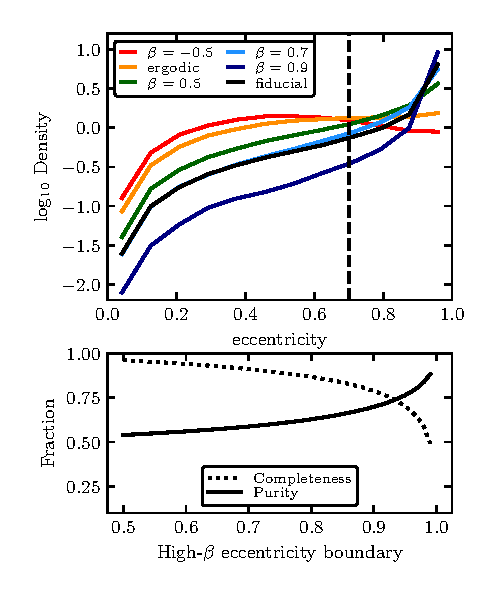
\includegraphics[width=0.6\textwidth]{figure/ch2/APOGEEHaloEccentricityDistribution.pdf}
    \caption{\textit{Top:} eccentricity distribution for the halo samples of each of the six models in the \survey\ sample set. The dashed line marks eccentricity=0.7, a traditional boundary between the ergodic and high-$\beta$ halo populations. \textit{Bottom:} purity and completeness of the high-$\beta$ samples with respect to the ergodic samples in the fiducial halo model of the \survey\ sample set. The quantities are expressed as a function of the cutoff boundary in eccentricity.}
    \label{ch2:fig:EccentricityDistributions}
\end{figure}

Notably, when the eccentricity cuttoff is 0.7 the purity of the high-$\beta$ sample is only 0.59, with the completeness being 0.91. This is a remarkable amount of confusion between these two samples. Recall that the high-$\beta$ purity of the entire fiducial sample is 0.5 by definition, and an eccentricity threshold of 0.7 does little to improve that. When the eccentricity cuttoff is increased to 0.9, the purity rises to 0.7 and the completeness is reduced to 0.79. Even at the largest value we consider for the eccentricity cuttoff, 0.99, the purity only reaches 0.88 (roughly in accordance with our variation of ellipses analysis in the previous section), and the completeness is reduced to 0.49. Note that while this purity and completeness appear superior to those of the action diamond we are wary of advocating for a selection boundary at extreme eccentricity lest it be too specific to our models, but it may be indicative of a good option for certain analyses. Nonetheless these results clearly indicate that care need be taken when separating high-$\beta$ and ergodic populations on the basis of eccentricity alone.

\section{Discussion}
\label{ch2:sec:Discussion}

The data and results we present in this paper are clearly useful to discuss in the context of a large fraction of the literature on Milky Way stellar dynamics done in the \textit{Gaia} era, specifically those which focus on the stellar halo. Here we focus on discussing the takeaways we deem are most salient, and how they relate to the wide body of literature.

\subsection{The Validity and Applicability of our Models}

First, we must assess how good the models we have presented are at representing the Milky Way halo as we understand it to be today. From a theoretical perspective, our models are clearly a simplification. For example, it is now well-known that the Milky Way stellar halo is effectively described by a metallicity-dependent triaxial power law density profile \parencite[e.g.,][]{mackereth20}. Our models at least have a power law index and cuttoff radius which match observations. But more complicated models are limited by the availability of usable DFs. Additionally, the Milky Way stellar halo is unlikely to currently be in a completely relaxed state, with perturbations from nearby massive dwarf galaxies in various stages of merging \parencite{garrow20}, and specifically the Large Magellanic Cloud \parencite{erkal19}. Fortunately for us these effects are greatest in the outer halo, with dynamical times in the inner halo where our sample is concentrated being short enough such that these perturbers do not meaningfully impact the equilibria.

A better method of addressing the validity of our models is to take an empirical approach and compare the kinematics of our samples with real observed stellar kinematics. For example, when considering the fiducial \survey\ model, the $v_{R}-v_{T}$ planes of \textcite{belokurov18,fattahi19,naidu20}, the Toomre diagram of \textcite{helmi18,koppelman19b}, the $E-L_{z}$ plane of \textcite{helmi18,koppelman19b,naidu20}, and the action diamond of \parencite[normalized to be a circle, ][]{naidu20} all show similarities with the samples produced by our models. Note that there can and should be disimilarities between these kinematics, which arises from the use of different gravitational potentials to calculate the kinematic properties, and varying underlying positional distributions. But overall, on the basis of kinematic properties, our samples are largely consistent with what is seen in real observational data.

Another detail we must address is how well these types of DFs represent the high-$\beta$ stellar halo associated with the debris of GS/E. This is important given that we spent a great deal of time in \S~\ref{ch2:sec:PurityOfPopulations} presenting regions of phase space that uniquely identified high-$\beta$ samples with high purity, with the implication that if we applied these to real data they would serve to identify GS/E stars. Generalized DFs corresponding to merger debris located in a stellar halo have not been formulated. This is mostly because the orbit and mass ratio of the merging galaxy would play a major role in determining the resulting DF. It is reasonable to assume, however, that the corresponding DF should be somewhere between that of a thin tidal stream occupying a distinct locus in action space \parencite[e.g.][]{bovy14}, and the spherical DFs we have used here. It should also be the case that longer timescales and larger mass ratio mergers tend to make the DF of the debris resemble the latter, rather than the former. With this in mind we believe it reasonable to assume that the GS/E merger debris should resemble a roughly spherical, halo-like DF. This assertion is supported by a wide range of evidence, including that: the GS/E debris is distributed over the whole sky \parencite[see Figure 12 in ][]{helmi20}, the GS/E debris can be described by a triaxial power law density profile \parencite{mackereth20}, and that measured stellar ages indicate GS/E was accreted roughly 10~Gyr ago \parencite{montalban21}, giving the debris ample time to relax.

Additionally, we can look to simulations to further validate our models, and specifically to support our use of high-$\beta$ halo DFs to model the GS/E remnant. \textcite{amorisco17} presents the kinematic properties of debris from a number of simulated mergers parameterized by the mass ratio and orbit circularity of the infalling satellite. They show that the deposited stellar debris has a power law density profile, with some appearance of a cuttoff radius around a few halo scale radii, and the degree of radial bias is high. These facts together support the use of a spherical, radially biased halo DF to model the remnants. \textcite{jean-baptiste17} present a series of 1:10 merger simulations which show that the $E-L_{z}$ distribution of the deposited stars is broadly consistent with our high-$\beta$ halo models. They show cusps around $L_{z}=0$ and are roughly bound by extended funnel shaped boundaries. Most of these mergers have a significant degree of angular momentum to them though, which manifests in the skewed appearance of the $E-L_{z}$ distribution.

\subsection{Selection Criteria for \textit{Gaia}-Enceladus}

In \S~\ref{ch2:sec:PurityOfPopulations}, we explored the feasibility of using kinematics alone to separate high-$\beta$ populations from low-$\beta$ and disc contaminants within the framework of our fiducial model. We found that most kinematic spaces had regions of high purity, and using well-informed selections, we were able to achieve simultaneously high purity ($\gtrsim 0.7$) and relatively high completeness ($\gtrsim 0.2$). Our main goal in providing these assessments of purity and completeness is to inform and enable identification of GS/E stars on the basis of kinematics alone. Chemical and stellar properties of GS/E constituent stars are of significant interest currently, as they tell us a great deal about the progenitor dwarf galaxy. Since it is not obvious \textit{a priori} what these properties are in the context of the broader stellar halo, it is necessary to develop accurate methods to extract GS/E stars from larger samples of halo and disc stars. It is for this reason that throughout this paper, we have placed more emphasis on achieving high purity when it comes to separating low- and high-$\beta$ populations, than on completeness. In general we recommend using the action diamond, which achieves a high purity. If completeness is of interest we recommend the $e-L_{z}$ plane, which achieves high completeness while keeping purity high.

The selection criteria we present are based upon a number of key assumptions. First, we assume that the ratio of high-$\beta$ to low-$\beta$ stars in the halo is 1:1. While it is clear that these components exist in roughly equal proportion near the solar neighbourhood \parencite{belokurov18,lancaster19,iorio21}, the exact ratio is uncertain, and is subject to variation with radius \parencite{iorio21}. We explore possible variations in this ratio by repeating our analysis with high- to low-$\beta$ ratios of 3:7 and 7:3. We find that this variation does not significantly change where we would place the selection ellipses for any kinematic space. As one might expect, the purity of the high-$\beta$ selection varies with the fraction of high-$\beta$ stars. For example, the purity without disc contamination of our action diamond selection applied to the \survey\ sample drops to 0.70 when the high- to low-$\beta$ ratio is 3:7, and increases to 0.93 when it is 7:3.

Another assumption built into our model is the use of the \texttt{MWPotential2014} potential of \textcite{bovy14}. Notably, this potential has light dark matter halo (virial mass of $8\times10^{11}$~\Msun) when compared to other Milky Way potentials used in the literature. We repeat our analysis using the potential of \textcite{mcmillan17}, which has a heavier dark matter halo ($1.2\times10^{12}$~\Msun virial mass) and a slightly larger circular velocity at the location of the sun ($\sim 233$~km~s$^{-1}$). We find next to no differences in our findings using this potential, save for an overall shift in the magnitude of the energies (reflecting the heavier potential) and a barely perceptible increase in the extent of the distribution of the radially sensitive parameters ($v_{R}$, $v_{\mathrm{perp}}$, energy, and $\sqrt{J_{R}}$). This suggests that the selection of high-$\beta$ halo stars is agnostic to any choice of reasonable Milky Way potential.

We also emphasize that these selection are derived using our \survey\ sample set, which is based on the positions of APOGEE DR16 data. While we would not expect the distribution of kinematic properties to change drastically were it based on another survey, there would undoubtedly be noticeable changes. We attempt to gauge how resilient our choice of selections are to a change in the radial distribution of the data by examining the kinematics of samples with $R<7$~kpc,  $7>R>9$~kpc and $R>9$~kpc. In terms of the halo samples, we see clear trends regarding the location of the high-purity regions in each kinematic space. The regions tend to have a wider extent in $L_{z}$ with increasing radius, while the extent of radially sensitive quantities (specifically $E$, $e$, $\sqrt{J_{R}}$, and $(J_{z}-J_{R})/J_{tot}$) increases with decreasing radius. The velocity spaces appear largely unchanged. While it does not appear that the ideal center of the selection ellipses should change with varying radius, their ideal extents should change in a manner reflecting these observed trends. With regards to the disc sources, we observe a slightly different trend. Samples at smaller radii have $L_{z}$ distributions which lie closer to the $L_{z}=0$ / $v_{T}=0$ line where the high-purity halo sample region lies. This would allow the high-$\beta$ selection ellipses to stretch towards lower values of the radially sensitive quantity in each kinematic space. The extent of the radially sensitive quantities for the disc samples also changes, but not in a manner that impacts the regions of high halo purity. We do note that the purity and completeness of many of the selections we have discussed in this work does appear to change by up to $\sim~20$ per cent, but we consider it outside the scope of this work to delve into the radial trends of the completeness and purity for each kinematic space and simply leave this as a cautionary note.

In \S~\ref{ch2:subsec:SampleKinematics} we asked whether higher dimensional spaces would be useful for studying the types of kinematic populations we consider in this work. There, we argued that there are really three broad classes of kinematic quantities that we consider here: those sensitive to tangential motions ($v_{T}$ and $L_{z}$), those sensitive to radial motions ($v_{R}$, $v_\mathrm{perp}$, energy, and $\sqrt{J_{R}}$), and those sensitive to the shape of an orbit (eccentricity and $(J_{z}-J_{R})/J_\mathrm{tot})$. Within each of these categories the parameters tend to communicate similar sorts of information, meaning their combination would not be useful and only serve to complicate by increasing dimensionality. For the most part this assertion has been borne out by our results. When we tested combining selections for spaces from within these same categories we find that, in general, purity will remain unchanged, while completeness will decrease (likely owing to the increased dimensionality). For example, when combining the selections for the $v_{R}-v_{T}$ and Toomre spaces the completeness and purity without (with) disc contamination are 0.12 and 0.76 (0.76) respectively. This is essentially identical to the selection which uses just $v_{R}-v_{T}$, suggesting that every point within the smaller (less complete) $v_{R}-v_{T}$ selection also lies within the larger (more complete) Toomre selection; their combination adds no new information. As another example, when $\sqrt{J_{R}}-L_{z}$ selection is combined with the Toomre selection the purity is the same as if one just used the $\sqrt{J_{R}}-L_{z}$ selection yet the completeness falls to 0.13 from 0.52. 

When combining the best quantities from each of the three categories: the action diamond and the $\sqrt{J_{R}}-L_{z}$ plane, the purity is the same as the combination of the action diamond with the $e-L_{z}$ plane (0.86), but the completeness falls to 0.33 (again, likely due to increased dimensionality). As mentioned above, we do find that these composite selections tend to erase any disparity between the purity with and without disc contamination. This improvement is marginal however, the purity including disc contamination of the action diamond, for example, only increases from 0.85 to 0.86 when combining it with $\sqrt{J_{R}}-L_{z}$. We do note that combining the action diamond and $e-L_{z}$ selections also increases the purity including disc contamination to 0.86, but keeps the completeness at 0.39. These results indicate that higher dimensional spaces do not appear to do a better job of separating high- and low-$\beta$ halo populations. They do appear to help in separating halo and disc populations, however, yet the selections we create in the scaled kinematic spaces (action diamond and $e-L_{z}$) are relatively immune from disc contamination to begin with. This result makes sense when considering that disc and halo stars do genuinely have a large difference in the magnitude of their radial motions, whereas it is characteristically the shape of the orbit which distinguishes a star from a low- versus high-$\beta$ population. In other words, there are very few stars in halo populations which have radial motions of a large magnitude, yet their orbit is not radial in shape, and so two dimensional spaces suffice to separate the two populations. 

A final comment, we recognize that our choice of selection regions in each kinematic space is subjective, even though we have endeavoured to provide what we believe are the best choices. We are explicit though in that we favour selections which give a higher purity at a modest expense in completeness, and we also prefer selections which have minimal contamination from disc populations. Nonetheless, other selections which prioritize, for example, completeness over purity may be equally as valid or better for other use cases. In an effort to communicate this tradeoff we plot the purity and completeness as a function of ellipse scale parameters. Figure~\ref{ch2:fig:SurveyADCompletenessPurity} shows the performance of the \survey\ sample action diamond selection as the selection ellipse semi-major axes are modified. Purity, purity including disc samples, and completeness are all shown. As the selection ellipse becomes larger the purity decreases while the completeness increases, as expected.

\begin{figure}
    \centering
    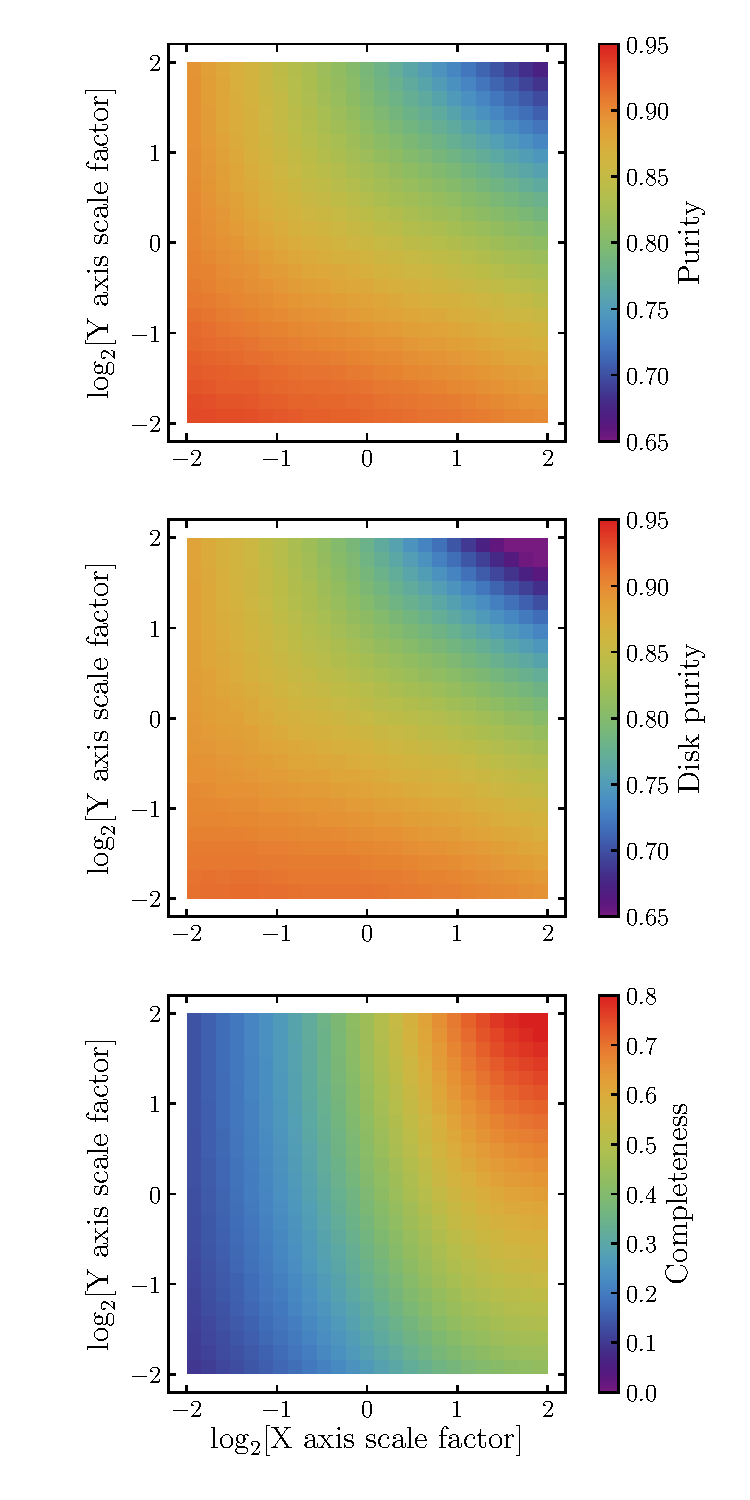
\includegraphics[width=0.5\textwidth]{figure/ch2/SurveyADCompletenessPurity.pdf}
    \caption{Selection performance as a function of ellipse scale parameters for the \survey\ sample and action diamond space. The three panels show purity (top), purity including disc samples (middle), and completeness (bottom). The scaling factors modify the default action diamond selection ellipse for the \survey\ sample from Table~\ref{ch2:tab:HighBetaSelections}.}
    \label{ch2:fig:SurveyADCompletenessPurity}
\end{figure}


\subsection{Comparison with Literature Selection Criteria}

There already exist selection criteria used in the literature to define the boundaries of GS/E for chemical and stellar property assays. Here we compare our results with some of the more common selections. For reference, our benchmark selection is the union of our action diamond selection ellipse and $e-L_{z}$ selection ellipse (although as we have mentioned this is very similar to the action diamond selection alone). For the \survey\ sample (the most apt sample set for comparison), the purity of this selection without (with) disc contamination is 0.86 (0.86) and the completeness is 0.39. In order to compare other selections in the fairest manner we evaluate purity and completeness for them using our fiducial \survey\ model. We will quote purity both with and without disc contaminants, but it is important to keep in mind that disc stars may also be efficiently removed from a sample using abundances.

First, we consider the selection criterion of \textcite{feuillet20}, which is also used in \textcite{matsuno21}, and is defined as $\sqrt{J_{R}} > 30$ kpc$^{1/2}$~km$^{1/2}$~s$^{1/2}$ and $\lvert L_{z} \rvert < 500$ kpc~km~s$^{-1}$. The completeness and purity without (with) disc contaminants of this selection are 0.31 and 0.72 (0.70). Second is the selection of \textcite{myeong19}, also used by \textcite{monty20} and \textcite{cordoni20}, which is defined as $\lvert J_{\phi}/J_\mathrm{tot} \rvert < 0.07$ and $(J_{z}-J_{R})/J_\mathrm{tot} < -0.3$. The completeness and purity without (with) disc contaminants of this selection are 0.58 and 0.82 (0.82). A final selection criterion to consider is that of \textcite{naidu20}, based off of \textcite{belokurov18} and similar in spirit to \textcite{mackereth20}, which is defined as $e>0.7$. We note specifically that \textcite{naidu20} apply this criteria to their data only after removing a subset of the halo corresponding to the Sagittarius dwarf and the hot thick disc. The completeness and purity without (with) disc contaminants of this selection are 0.91 and 0.59 (0.37), as per \S~\ref{ch2:subsec:EccentricityHaloSeparation}.

Our intent here is not to critique the selection criteria of these studies, but instead to provide an unbiased characterization of their performance in the context of our models. What we see from this comparison, and indeed our study in general, is that when one is kinematically separating high-$\beta$ populations from ergodic populations there is a tradeoff between purity and completeness. If one's interest is in maximal purity of a high-$\beta$ population, then the selection criteria we have provided are best, specifically the union of our action diamond and $e-L_{z}$ selections.

\subsection{Structure Identification}

One of the most remarkable emergent features of our \survey\ models was the appearance of artificial substructure in the distribution of halo samples in the $E-L_{z}$ plane. The substructure is symmetric about the $L_{z}=0$, and appears as a small overdensity of stars at low energies. The fact that this feature appears in our simple halo models defined by a single truncated power law density profile embedded in a sphericalized Milky Way emphasizes that it is entirely spurious. We thoroughly explored this phenomenon in \S~\ref{ch2:subsec:RadialBiases}, and found it to be caused by a bimodality in the underlying radial distribution of APOGEE DR16 likely halo stars. Many stars are concentrated near the location of the Sun, about 8~kpc from the center, and many are concentrated also at about 3.5~kpc in radius. The cause of this bimodality is twofold. First, many pointings glance the Galactic bulge (see Figure~\ref{ch2:fig:APOGEELocations}), which means there is a concentration of halo stars just on its outskirts which share a galactocentric radius, but have differing galactocentric azimuth. Second, pointings towards the Galactic bulge contribute the most halo stars right on the outskirts of the bulge, as opposed to near the Sun, since observed volume scales with the square of the distance from us, and the density of halo stars should be centrally concentrated.

This is a particularly pertinent result given that the $E-L_{z}$ plane is often used as a means of structure identification \parencite[e.g.][]{helmi18,koppelman19b,horta21a}, and therefore we strongly recommend that authors consider the selection biases present in their samples when attempting to verify the nature of newly discovered substructures. This is especially important for any survey with a non-trivial spatial selection function, which includes essentially all modern spectroscopic surveys. Furthermore, while the density fluctuations we observe are symmetric about the $L_{z}=0$ axis, we have the clarity of being able to separate halo stars from disc stars. This is not a luxury afforded to most samples, which will also contain contamination from disc stars. These contaminants would potentially hide the symmetric nature of structure that arises thanks to the types of radial selection biases we explore here. This could result in, for example, the density fluctuations being observed in the lower density retrograde half of the plane but not the prograde half where they could be masked by disc contaminants.

We specifically highlight the case of the newly discovered Heracles structure in the inner Galactic halo by \textcite{horta21a} for two reasons. First, they also use the APOGEE DR16 data that underpins our models. Second, the structure they identify shares many features in common with the artifacts we find. This is to say that Heracles is roughly symmetric about the $L_{z}=0$ axis, and it appears as a separate overdensity of stars at lower energies than the primary group of halo stars. We suggest that the structure be further investigated to confirm that it does not appear as a result of the APOGEE selection function.

In a similar vein, a potentially useful application of the sorts of models we have presented here, is to use them for the differential identification of substructures in both the disc and stellar halo. Because our models use simple, smooth underlying potentials, they can be used to generate phase space realizations of those smooth potentials which can be compared with observations. The advantage of this approach is that it would be relatively simple to account for the types of selection effects we just highlighted, because phase space need only be sampled at the locations where the real data are found. A major challenge of this approach is determining the impact of assuming the nature of the underlying potential, but this could be circumvented to a degree by comparing many different potentials.

\section{Conclusion}

In this work, we have demonstrated a framework for assessing the kinematic properties of the types of composite stellar populations which are observed by modern spectroscopic surveys complemented by \textit{Gaia} kinematics. Our methodology relies on a simple, DF-based approach to generate mock kinematics for both solar-vicinity and APOGEE DR16 data using \texttt{galpy}, and would be simple to replicate for other surveys. We therefore suggest that these sorts of models be created for many different surveys in order that their unique kinematic distributions and underlying selection effects can be properly gauged.

We provide a general overview of many kinematic spaces commonly used in the study of the Milky Way, and specifically the stellar halo. In each kinematic space, we show two sets of models: the \solar\ models which are simple and mimic stellar samples concentrated near the Sun, and the \survey\ models which are more complicated and designed to mimic samples observed with spectroscopic surveys. Each model uses a stellar halo parameterized by the anisotropy: $\beta$, which is a useful quantity for describing the two dominant stellar halo populations in the Milky Way: the low-$\beta$ metal poor halo and the high-$\beta$ GS/E remnant.

In each kinematic space we use our models to show where disc populations, low- and high-$\beta$ halo populations all lie. We use purity as a metric to specifically assess each space on how well it separates low-$\beta$ halo populations from high-$\beta$ populations, finding that the scaled action diamond, the $\sqrt{J_{R}}-L_{z}$ plane, and $e-L_{z}$ plane achieve highest performance, with a focus on purity. These results assume a 1:1 ratio of low- and high-$\beta$ populations in the stellar halo, and also use APOGEE DR16 data as a set of positions for the phase space samples. Despite these constraints we believe our choice of selection regions in each kinematic space is resilient to changes in these and other underlying assumptions. While the location of the best selection regions is resilient to changes in assumptions, the specific purity and completeness values are liable to change. We therefore recommend that other authors generate their own completeness and purity corrections for their data if the specific values are needed. We briefly explored the effects of survey selection functions on kinematic properties of observed samples, finding that they can result in the appearance of specious structures.

We summarize this work with a number of recommendations for authors to consider as they explore current and future datasets:

\begin{itemize}
    \item The scaled action diamond, $e-L_{z}$ plane, and $\sqrt{J_{R}}-L_{z}$ plane are best for separating high- and low-$\beta$ populations. We provide a number of simple-to-implement selection criteria (see Table~\ref{ch2:tab:HighBetaSelections}) for separating high- and low-$\beta$ populations in each kinematic space we study.
    
	\item If high purity is most important when separating low- and high-$\beta$ populations, then we recommend using our action diamond selection. It achieves a purity without (with) disc contamination of 0.86 (0.85) and completeness of 0.39. Combining the action diamond selection with the $e-L_{z}$ selection increases the purity with disc contamination to 0.86, while keeping the completeness constant at 0.39.
    
    \item If high completeness is most important when separating low- and high-$\beta$ populations, then we recommend using our $e-L_{z}$ selection. It achieves a purity without (with) disc contamination of 0.82 (0.82) and completeness of 0.61. We also show the purity and completeness of a wide range of selection ellipse sizes for the action diamond, to illustrate how completeness may be increased for that selection given a tradeoff in purity.
   
    \item If invariance to choice of Milky Way potential is most important when separating low- and high-$\beta$ populations, then we recommend using the $v_{R}-v_{T}$ plane, which outperforms the Toomre diagram.
    
    \item In general, the $E-L_{z}$ plane and Toomre diagram do not do as good a job of separating low- and high-$\beta$ populations. Additionally, we recommend that caution be exercised using eccentricity by itself for this purpose. Commonly used eccentricity cuts for the radially anisotropic halo, such as $e\sim0.7$ only result in a sample with purity of 0.59. Only extreme eccentricity cuts ($e \gtrsim 0.95$) achieve good purity.
    
    \item Be aware of all selection biases in the underlying sample, which can cause spurious structures to appear in kinematic spaces with explicit dependencies on radius, specifically in the $E-L_{z}$ plane. We show that in APOGEE DR16, a bias in the underlying Galactocentric radial distribution of sources results in the appearance of artifacts in the $E-L_{z}$ plane which could be easily mistaken for real substructure.
\end{itemize}

% \section*{Acknowledgements}

% JMML and JB acknowledge financial support from NSERC (funding reference number RGPIN-2020-04712) and an Ontario Early Researcher Award (ER16-12-061). This work has made use of data from the European Space Agency (ESA) mission
% {\it Gaia} (\url{https://www.cosmos.esa.int/gaia}), processed by the {\it Gaia}
% Data Processing and Analysis Consortium (DPAC,
% \url{https://www.cosmos.esa.int/web/gaia/dpac/consortium}). Funding for the DPAC
% has been provided by national institutions, in particular the institutions
% participating in the {\it Gaia} Multilateral Agreement. Funding for the Sloan Digital Sky Survey IV has been provided by the Alfred P. Sloan Foundation, the U.S. Department of Energy Office of Science, and the Participating Institutions. SDSS-IV acknowledges support and resources from the Center for High-Performance Computing at the University of Utah. The SDSS web site is \url{www.sdss.org}.

%%%%%%%%%%%%%%%%%%%%%%%%%%%%%%%%%%%%%%%%%%%%%%%%%%
% \section*{Data Availability}
 
% The APOGEE DR16 data used in this article are available at: \url{https://www.sdss.org/dr16}. The \textit{Gaia} data used in this article are available at: \url{https://gea.esac.esa.int/archive/}.

%%%%%%%%%%%%%%%%%%%% REFERENCES %%%%%%%%%%%%%%%%%%

% The best way to enter references is to use BibTeX:
% \bibliographystyle{mnras}
% \bibliography{manuscript}

% %%%%%%%%%%%%%%%%%%%%%%%%%%%%%%%%%%%%%%%%%%%%%%%%%%


% % Don't change these lines
% \bsp	% typesetting comment
% \label{lastpage}
% \end{document}

% % End of mnras_template.tex




% Chapter 3 - Project #2: The stellar mass of Gaia-Enceladus/Sausage
% \chapter{The stellar mass of \textit{Gaia}-Sausage/Enceladus}


% % mnras_template.tex 
%
% LaTeX template for creating an MNRAS paper
%
% v3.0 released 14 May 2015
% (version numbers match those of mnras.cls)
%
% Copyright (C) Royal Astronomical Society 2015
% Authors:
% Keith T. Smith (Royal Astronomical Society)

% Change log
%
% v3.0 May 2015
%    Renamed to match the new package name
%    Version number matches mnras.cls
%    A few minor tweaks to wording
% v1.0 September 2013
%    Beta testing only - never publicly released
%    First version: a simple (ish) template for creating an MNRAS paper

%%%%%%%%%%%%%%%%%%%%%%%%%%%%%%%%%%%%%%%%%%%%%%%%%%
% Basic setup. Most papers should leave these options alone.
% \documentclass[fleqn,usenatbib]{mnras}

% % MNRAS is set in Times font. If you don't have this installed (most LaTeX
% % installations will be fine) or prefer the old Computer Modern fonts, comment
% % out the following line
% \usepackage{newtxtext,newtxmath}
% % Depending on your LaTeX fonts installation, you might get better results with one of these:
% %\usepackage{mathptmx}
% %\usepackage{txfonts}

% % Use vector fonts, so it zooms properly in on-screen viewing software
% % Don't change these lines unless you know what you are doing
% \usepackage[T1]{fontenc}

% % Allow "Thomas van Noord" and "Simon de Laguarde" and alike to be sorted by "N" and "L" etc. in the bibliography.
% % Write the name in the bibliography as "\VAN{Noord}{Van}{van} Noord, Thomas"
% \DeclareRobustCommand{\VAN}[3]{#2}
% \let\VANthebibliography\thebibliography
% \def\thebibliography{\DeclareRobustCommand{\VAN}[3]{##3}\VANthebibliography}


% %%%%% AUTHORS - PLACE YOUR OWN PACKAGES HERE %%%%%

% % Only include extra packages if you really need them. Common packages are:
% \usepackage{graphicx}	% Including figure files
% \usepackage{amsmath}	% Advanced maths commands
% \usepackage{array}
% \usepackage[table,x11names]{xcolor}
% % \usepackage{amssymb}	% Extra maths symbols

%%%%%%%%%%%%%%%%%%%%%%%%%%%%%%%%%%%%%%%%%%%%%%%%%%

%%%%% AUTHORS - PLACE YOUR OWN COMMANDS HERE %%%%%

% Please keep new commands to a minimum, and use \newcommand not \def to avoid
% overwriting existing commands. 
% \newcommand{\Msun}{\ensuremath{\mathrm{M}_{\odot}}}
% \newcommand{\eLz}{$e-L_\mathrm{z}$}
% \newcommand{\JRLz}{$\sqrt{J_\mathrm{R}}-L_\mathrm{z}$}

% Alias citations
% \defcitealias{lane22}{LBM22}
% \defcitealias{mackereth20}{MB20}

% Editing commands
% \newcommand{\james}[1]{ {\color{red} #1 } }
% \newcommand{\jo}[1]{ \textbf{{\textcolor{blue}{Jo asks/comments: #1}}}}

%%%%%%%%%%%%%%%%%%%%%%%%%%%%%%%%%%%%%%%%%%%%%%%%%%

%%%%%%%%%%%%%%%%%%% TITLE PAGE %%%%%%%%%%%%%%%%%%%

% Title of the paper, and the short title which is used in the headers.
% Keep the title short and informative.
% \title[The stellar mass GS/E]{The stellar mass of the \textit{Gaia}-Sausage/Enceladus accretion remnant}

% The list of authors, and the short list which is used in the headers.
% If you need two or more lines of authors, add an extra line using \newauthor
% \author[J. M. M. Lane et al.]{
% James M. M. Lane$^{1}$\thanks{E-mail: lane@astro.utoronto.ca},
% Jo Bovy$^{1}$, \&
% J. Ted Mackereth$^{1,2,3}$
% \\
% % List of institutions
% $^{1}$David A. Dunlap Department of Astronomy and Astrophysics, University of Toronto, 50 St. George Street, Toronto ON, M5S 3H4, Canada\\
% $^{2}$Canadian Institute for Theoretical Astrophysics, University of Toronto, 60 St. George Street, Toronto ON, M5S 3H8, Canada\\
% $^{3}$Dunlap Institute for Astronomy and Astrophysics, University of Toronto, 50 St. George Street, Toronto ON, M5S 3H4, Canada
% }

% These dates will be filled out by the publisher
% \date{Accepted XXX. Received YYY; in original form ZZZ}

% % Enter the current year, for the copyright statements etc.
% \pubyear{2023}

% % Don't change these lines
% \begin{document}
% \label{firstpage}
% \pagerange{\pageref{firstpage}--\pageref{lastpage}}
% \maketitle

% Abstract of the paper
\section{Abstract}
The \textit{Gaia}-Sausage/Enceladus (GS/E) structure is an accretion remnant which comprises a large fraction of the Milky Way's stellar halo. We study GS/E using high-purity samples of kinematically selected stars from APOGEE DR16 and \textit{Gaia}. Employing a novel framework to account for kinematic selection biases using distribution functions, we fit density profiles to these GS/E samples and measure their masses. We find that GS/E has a shallow density profile in the inner Galaxy, with a break between 15--25~kpc beyond which the profile steepens. We also find that GS/E is triaxial, with axis ratios 1:0.55:0.45 (nearly prolate), and the major axis is oriented about 80~degrees from the Sun--Galactic centre line and 16 degrees above the plane. We measure a stellar mass for GS/E of $1.45\,^{+0.92}_{-0.51}\,\mathrm{(stat.)}\,^{+0.13}_{-0.37} \mathrm{(sys.)}\ \times10^{8}$~\Msun. Our mass estimate is lower than others in the literature, a finding we attribute to the excellent purity of the samples we work with. We also fit a density profile to the entire Milky Way stellar halo, finding a mass in the range of $6.7-8.4 \times 10^{8}$~\Msun, and implying that GS/E could make up as little as 15-25~per~cent of the mass of the Milky Way stellar halo. Our lower stellar mass combined with standard stellar-mass-to-halo mass relations implies that GS/E constituted a minor 1:8 mass-ratio merger at the time of its accretion. 

% We discuss our findings in the context of sample selection and kinematic models of GS/E. Our results are an important milestone in the understanding of the GS/E progenitor, and our demonstration of a density modelling framework which includes kinematics represents an important step forward in the broader effort to dissentangle the Milky Way stellar halo.
% \section{Abstrac}

% Select between one and six entries from the list of approved keywords.
% Don't make up new ones.
% \begin{keywords}
% Galaxy: halo -- Galaxy: structure -- Galaxy: kinematics and dynamics -- Galaxy: stellar content
% \end{keywords}

%%%%%%%%%%%%%%%%%%%%%%%%%%%%%%%%%%%%%%%%%%%%%%%%%%

%%%%%%%%%%%%%%%%% BODY OF PAPER %%%%%%%%%%%%%%%%%%

\section{Introduction}

In our $\Lambda$CDM Universe, in which structure is arranged hierarchically, the constituent mass of a galaxy like the Milky Way grows largely due to accretion of smaller nearby structures, which supply gas, stars, and dark matter to the gravitationally dominant host \parencite{searle78,white91,helmi99,bullock05}. One of the best records of these accretion processes lies in the distribution and arrangement of stars in the Milky Way halo, which have comparatively dissipationless kinematics and have therefore retained signatures of the events which brought them into the Galaxy \parencite{freeman02,johnston08}. Mergers play an outsized role in shaping our Galaxy beyond its stellar and dark halo, and are thought to contribute to the formation or evolution of the bulge, bar, disk, as well as the generation of past and ongoing instabilities and perturbations to these stellar components \parencite[][]{bland-hawthorn16,helmi20}. An inventory of the stellar constituents of the Milky Way halo is therefore crucial to understanding the role of mergers in the broader context of the formation and evolution of our Galaxy.

The combination of astrometric data from the \textit{Gaia} mission \parencite{gaia} and large ground-based spectroscopic surveys such as SEGUE \parencite{segue}, APOGEE \parencite{apogee}, GALAH \parencite{galah}, LAMOST \parencite{lamost}, and H3 \parencite{h3}, has proved a boon for studying the Milky Way stellar halo. One of the most intriguing results of this new era is the detailed characterization using data from the second \textit{Gaia} data release of an apparent merger remnant, dubbed \textit{Gaia}-Sausage/Enceladus (GS/E), which dominates the nearby stellar halo \parencite{belokurov18,haywood18,helmi18}. While GS/E has been the subject of intense recent study, its synthesis can be traced back before the second \textit{Gaia} data release to the notion of a `dual' galactic halo based on its broken radial density profile and bimodal chemistry \parencite[e.g.][]{carollo07,nissen10,deason11,bonaca17,hayes18}. GS/E is characterized by a large group of stars on highly radial orbits, with near-zero angular momentum $L_\mathrm{z}$, a wide span of radial velocities, and high eccentricities. The remnant was quickly seen to comprise a significant fraction ($\approx$ 50~per~cent) of the density of the nearby stellar halo \parencite{belokurov18,fattahi19,lancaster19}, and initial estimates of the stellar mass of the progenitor were quite high, ranging from $6\times10^{8}$ to nearly $10^{10}$ \Msun\ \parencite{helmi18,belokurov18,vincenzo19,feuillet20,fattahi19,myeong19,das20}. The simplest interpretation of this accretion remnant is that it was deposited during a massive, head-on merger event early in the life of the Milky Way \parencite{helmi18,belokurov18,iorio19,deason19,fattahi19,mackereth19a}. Although other works have argued that the observed chemodynamics are also consistent with multiple smaller accretion events \parencite{donlon22,donlon23}.

Recent, thorough studies of the GS/E accretion remnant focusing on its density profile have tended to settle on a lower stellar mass for the progenitor in the range $3\times10^{8}$ to nearly $10^{9}$~\Msun\ \parencite{mackereth19a,mackereth20,naidu21,han22}. Additionally, the chemical composition of the remnant has received attention, and specifically its [Fe/H] abundance distribution (which extends to high [Fe/H] $\sim -0.6$) as well as its [$\alpha$/Fe] distribution, both of which appear to reflect those of a massive dwarf galaxy \parencite{myeong19,monty20,mackereth19a,feuillet20,matsuno21,hasselquist21,buder22,gaiadr3_chemodynamics,horta23a}, supporting the earlier findings of an [Fe/H]-rich structure by \textcite{belokurov18} as well as pre-\textit{Gaia} second data release studies \parencite{nissen10,bonaca17,hayes18}. The ages of likely GS/E stars were measured by \textcite{montalban21} and found to be typically $10$~Gyr, supporting other works which have suggested a similar timeframe for the occurrence of the accretion episode ($z\approx2$). Our understanding of the kinematics of the remnant have been extended by \textcite{lancaster19} and \textcite{iorio21}, who measure a strong degree of radial anisotropy in the population, behaviour extending over a wide range of Galactocentric radii. \textcite{naidu21} and \textcite{chandra23} compare H3 data with tailored N-body simulations and develop a coherent narative for the specifics of the infall of the progenitor. They also link several other halo structures such as Arjuna \parencite{naidu20}, the Hercules-Aquila cloud, and the Virgo Overdensity with GS/E debris. The association of GS/E with the latter two structures was first proposed by \textcite{simion19}, with support coming from the analysis of stellar halo density profiles by \textcite{iorio19}, and has recently been affirmed through chemical analysis by \textcite{perottoni22}. Given the menagerie of recently discovered halo substructures \parencite[see ][ for censuses of the major ones]{helmi20,naidu21,horta23a}, there are open questions regarding which are unique and independent of GS/E, and which are associated with, or simply complex dynamical echoes of, GS/E. 

Recently, \textcite[][hereafter LBM22]{lane22} presented kinematic models of the nearby stellar halo based on distribution functions representing the major constituent populations: the metal-rich, radially anisotropic population attributed to GS/E, and the metal poor, comparatively radially isotropic population attributed to the (\textit{in-situ}) remainder of the stellar halo \parencite[e.g.][]{belokurov18,haywood18}. \cite{lane22} found that kinematic selection criteria commonly used to identify GS/E stars are subject to bias in the context of their models, and that most selection criteria are at best about 70~per~cent, and at worst about 50~per~cent pure (i.e., only 5-7 in every 10 stars attributed to GS/E are genuine members of the GS/E remnant). They also use their models to construct high-purity, scale-free (i.e., they are resilient to changes in stellar sample or gravitational potential used for calculation of kinematic quantities) selections for GS/E, which reach as high as 85~per~cent purity. \cite{lane22} highlight that while the GS/E remnant is an overdensity occupying a \textit{characteristic} region of phase-space, it is does not do so without contamination from other stellar populations. They emphasize the need to account for these effects when modelling the GS/E remnant, which is particularly important as studies seek to place tighter constraints on its properties.

In this study we will build on the work of \textcite[][hereafter MB20]{mackereth20} who studied the density profile of the stellar halo with data from \textit{Gaia} and the Apache Point Galactic Evolution Experiment \parencite[APOGEE][]{apogee}. We integrate the kinematic models of \cite{lane22} into the density modelling framework of \cite{mackereth20} so that we may select a high-purity sample of GS/E stars based on kinematics and directly assess the density profile and stellar mass of the remnant. Our novel method, using distribution function models in concert with density modelling, allows us to study the GS/E remnant unhindered by contaminated kinematic selections, and represents an important step towards future 6D modelling of the entirety of the stellar halo phase space.

This paper is laid out as follows: in Section~\ref{ch3:sec:data}, we describe our APOGEE and \textit{Gaia} observations and relevant sample selection procedures used to isolate high-purity samples of GS/E stars. In Section~\ref{ch3:sec:method}, we describe the density modelling framework, paying specific attention to the integration of distribution function models. We also thoroughly validate our new approach using mock data. In Section~\ref{ch3:sec:results}, we present the results of our analysis of the GS/E remnant, including fits to the whole stellar halo for comparison. In Section~\ref{ch3:sec:discussion}, we discuss results in the context of recent literature, and also address the limitations of our new modelling technique. We end in Section~\ref{ch3:sec:summary-conclusions} by summarizing our results and looking ahead to future applications of distribution functions to studies of the stellar halo.

\section{Data}
\label{ch3:sec:data}

\subsection{Observations and stellar properties}
\label{ch3:subsec:observations}

% APOGEE
We use data from APOGEE \parencite{apogee}, specifically the sixteenth data release \parencite[DR16][]{sdssdr16}, a component of the Sloan Digital Sky Survey IV \parencite[SDSS][]{sdss4}. We do not use the most recent APOGEE data as we prefer to use the same data as \cite{lane22}. APOGEE-1 \parencite[an SDSS III program;][]{sdss3} and its successor APOGEE-2 (an SDSS IV program) obtain high resolution (R $\approx 22,500$), near infrared ($1.51 \mu\mathrm{m} < \lambda < 1.7 \mu\mathrm{m}$), high signal-to-noise ($> 100$ per pixel) spectra using two near-identical spectrographs \parencite{apogee_spectrographs} at the 2.5~m Sloan Telescope \parencite{gunn06} at the Apache Point Observatory in New Mexico (APOGEE and APOGEE-2N) and the 2.5~m Ir\'en\'e du Pont Telescope \parencite{bowen73a} at the Las Campanas Observatory in Chile (APOGEE-2S). APOGEE DR16 contains observations of approximately 430,000 unique stars from both hemispheres, which span a range in Galactocentric radii and heights above and below the disk, including all major stellar populations of the Milky Way.

APOGEE targets are selected using 2MASS \parencite{2mass} photometry by a two-fold strategy, including stars targeted specifically for focused science goals and ancillary programs as well as the systematic observations of the `main' survey. Stars in the main survey are chosen based on their reddening-corrected \parencite{majewski11} $(J-K_\mathrm{S})_{0}$ colour and $H$-band magnitude from 2MASS. The targeting procedure is described by \textcite{apogee_targeting} for APOGEE-1, and built upon by \textcite{apogee2_targeting}, \textcite{apogee2n_targeting}, and \textcite{apogee2s_targeting} for APOGEE-2. Data are reduced using a pipeline originally described by \textcite{apogee_pipeline} but which has been built upon for recent data releases \parencite{holtzman18,jonsson20}. Throughout this paper we use stellar elemental abundances, atmospheric parameters, and radial velocities from the APOGEE Stellar Parameters and Chemical Abundances Pipeline \parencite[ASPCAP,][]{aspcap}. The pipeline uses a custom line list \parencite{apogee_linelist} which has been updated for DR16 \parencite{apogeedr16_linelist}, and a custom stellar spectral library \parencite{apogee_speclib} which has also been updated for DR16 \parencite{jonsson20}.

% Gaia
To complement the APOGEE data we use astrometry from the third data release \parencite[DR3;][]{gaiadr3} of the \textit{Gaia} space telescope \parencite{gaia}. We match our APOGEE data to the \textit{Gaia} DR3 catalogue using the CDS X-match service\footnote{\url{http://cdsxmatch.u-strasbg.fr/xmatch}} implemented in the \texttt{gaia\_tools}\footnote{\url{https://github.com/jobovy/gaia_tools}} python package. We specifically rely on \textit{Gaia} proper motions, as APOGEE provides more accurate radial velocities. We further use spectro-photometric distance estimates determined using the \texttt{astroNN} artificial neural network framework\footnote{\url{https://github.com/henrysky/astroNN}} \parencite{leung19a,leung19b}. We specifically take those distances from the SDSS DR17 \texttt{astroNN} Value Added Catalogue\footnote{\url{https://www.sdss4.org/dr16/data_access/value-added-catalogs/?vac_id=the-astronn-catalog-of-abundances,-distances,-and-ages-for-apogee-dr17-stars}}, which are obtained from a model trained on newer APOGEE DR17 and \textit{Gaia} eDR3 data \parencite[see ][]{sdssdr17}. The Bayesian artificial neural network predicts stellar luminosity using stellar spectra, and is trained on APOGEE spectra and \textit{Gaia} parallaxes. It simultaneously predicts distances and accounts for the \textit{Gaia} parallax zero-point. Distance uncertainties are typically less than 10~per~cent, much better than \textit{Gaia} parallaxes for stars further than a few kpc from the Sun.

% Subset of stars
We extract a high-quality subsample of APOGEE red giants from the broader dataset. First off, we only consider stars that are part of the APOGEE statistical sample, which are stars chosen randomly according to their $(J-K_\mathrm{S})_{0}$ colour and $H$-band magnitude as described above (i.e., they are not part of some ancilliary science program, or specifically targeted for some other reason). Stars from this group are chosen which have relative distance uncertainty, $\sigma_{d}/d$, less than 20~per~cent, surface gravity between $1 < \log g < 3$, and surface gravity uncertainty less than 0.1 dex. These giants must also have measured \textit{Gaia} proper motions and positions, they must have AstroNN distances, and they must have measured APOGEE radial velocities, [Fe/H], and [Al/Fe] abundances (Note that while we will show other abundances, only these are crucial to our analysis). We also remove stars lying in fields near the Galactic bulge, and those containing stars from globular cluster so that our sample contains only stars from the smooth component of the stellar halo. We enforce the first of these criteria by removing fields within $-20^{\circ} < \ell < 20^{\circ}$ and $|b| < 20^{\circ}$. The second of these criteria is met by first identifying any fields near the on-sky location of a known globular cluster from the \textcite[][December 2010 version]{harris96} catalog. For each of these fields, we examine the [Fe/H] and radial velocity distributions of the stellar constituents by eye to see if there is a noticeable enhancement of stars with properties similar to those of the cluster, paying specific attention to the region within two tidal radii of the cluster centre. Fields with a distinct group of stars with properties matching the cluster are entirely removed from consideration. Throughout the rest of the paper, we refer to this subset of APOGEE stars from the statistical sample as the `quality sample'; it contains 98,245 stars. The distribution of Galactocentric radii of this quality sample is shown in Figure~\ref{ch3:fig:radius_histogram}. The distribution is concentrated near the location of the Sun, about 8~kpc, and extends from 2~kpc to nearly 40~kpc.

\begin{figure}
    \centering
    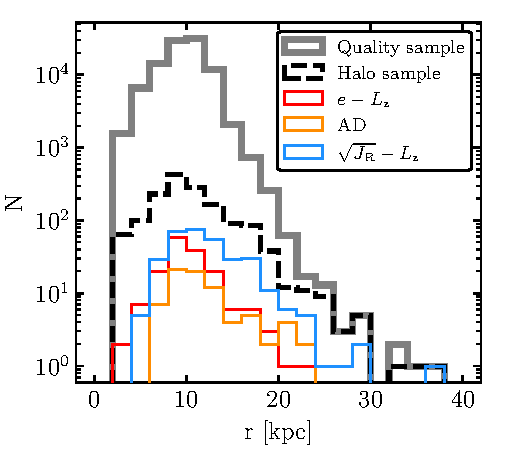
\includegraphics[width=0.5\textwidth]{figure/ch3/radius_histogram.pdf}
    \caption{Distribution in Galactocentric radii of various samples used in this work. The grey line shows the high quality stars from the statistical sample. The dashed black line shows our chemically-selected halo sample. The coloured lines show the high-purity GS/E subsets of the halo sample selected using the kinematic cuts of \cite{lane22}.}
    \label{ch3:fig:radius_histogram}
\end{figure}

% Calculation of kinematic properties
We calculate kinematic properties of the stars in our sample using \texttt{galpy}\footnote{\url{https://github.com/jobovy/galpy}} \parencite{bovy15}. Throughout, we assume that the Sun lies at Galactocentric coordinates $(R,z,\phi)$ = $(8.275~\text{kpc}, 0.028~\text{kpc}, 0)$ \parencite{gravity21,bennett19}, the peculiar solar motion is $(U,V,W) = (11.1, 12.24, 7.25)$~km~s$^{-1}$ \parencite{schoenrich10}, and that the circular velocity at the location of the Sun is 220~km~s$^{-1}$. We use a left-handed coordinate system such that angular momenta are positive in the direction of Galactic rotation. We use the \texttt{MWPotential2014} potential defined in \textcite{bovy15}, and calculate energy, actions, eccentricity, and orbital extrema for each star. Actions are calculated using the `St\"{a}ckel fudge' method of \textcite{binney12} whereby the Milky Way is locally approximated as a St\"{a}ckel potential using a focal length estimated with equation~9 of \textcite{sanders12}. Eccentricities are calculated using a method similar to St\"{a}ckel fudge presented in \textcite{mackereth18c}. We principally consider three kinematic spaces of the many which are commonly used in the study of the stellar halo. First is eccentricity as a function of z-axis angular momentum (\eLz). Second is the square root of the radial action versus z-axis angular momentum (\JRLz). Third is the action diamond (AD), which has the difference between the radial and vertical actions as a function of the z-axis angular momentum, but both quantities are normalized by the absolute sum of all three actions which leads to the characteristic diamond boundary in the space. For more information on the action diamond see section~3 of \cite{lane22} and references therein.

\subsection{The Halo and GS/E samples}
\label{ch3:subsec:halo-gse-samples}

% The halo subsample
From the quality sample, we identify likely halo stars according to their abundances. Broadly following \cite{mackereth20} and \cite{lane22}, we focus on the iron abundance, and specifically those stars with [Fe/H] $< -1$. The principle issue with this simple selection, however, is that GS/E is known to have [Fe/H] up to $\sim -0.6$ \parencite[e.g.][]{myeong19,monty20,hasselquist21,horta23a}. We therefore modify our selection to be more inclusive of GS/E, increasing our maximum [Fe/H] to $-0.6$. This introduces a different issue though, which is that a sample selected with this [Fe/H] limit would have substantial contamination from thin and thick disk populations. To mitigate this effect, we employ aluminum abundances which have been shown to reliably separate accreted halo and Galactic disk populations \parencite{hawkins15}. We take specific inspiration from \textcite{belokurov22} in constructing our [Al/Fe]-based selection (who also provides an illuminating discussion on the use of [Al/Fe] for this purpose), and note that several other recent works have employed similar selections, or demonstrated the separation of disk and accreted halo components on the basis of [Al/Fe] \parencite{das20,hasselquist21,horta23a}. Our selection is piecewise-continuous in the [Al/Fe] versus [Fe/H] plane. At [Al/Fe] $> -0.1$, we define the halo as [Fe/H] $< -1$. At [Al/Fe] $= -0.1$, the approximate boundary between accreted and \textit{in-situ} populations \parencite{hawkins15,das20,hasselquist21}, our selection increases in [Fe/H] to the locus ([Fe/H],[Al/Fe]) $= (-0.6,-0.3)$. Our selection then includes [Fe/H] $< -0.6$ for [Al/Fe] $< -0.3$.

This selection (dashed line), and the 1,523 halo stars from the quality sample chosen with it, are shown in the left panel of Figure~\ref{ch3:fig:halo_abundances}. The radial range of this sample is also shown as a dashed line in Figure~\ref{ch3:fig:radius_histogram}; it extends about as far as the quality sample. In Figure~\ref{ch3:fig:halo_abundances}, we display the stars defined as part of the halo sample in other abundance planes commonly used in the literature. The middle panel shows [Fe/H] versus [Mg/Fe], showing a large group of stars at high [Mg/Fe] and low [Fe/H] traditionally attributed to the \textit{in-situ} halo and thick disk, accompanied by an extended group at lower [Mg/Fe] and higher [Fe/H] which is emblematic of GS/E and other accreted populations \parencite[e.g.][]{hasselquist21,horta23a}. The solid lines are fiducials from other studies, the vertical line marks [Fe/H] $= -1$, which is the cutoff adopted by \cite{mackereth20}, and the sloped line is used by \textcite{mackereth19a} and \cite{lane22} to separate disk and halo populations. It is clear that these cuts, which rely predominantly on [Fe/H], would leave much of GS/E excluded from the sample. The right panel shows [Al/Fe] versus [Mg/Mn], which is used by some authors to separate accreted and \textit{in-situ} populations \parencite[e.g.][]{das20,horta21a,fernandez23}. The upper left region of the diagram is where unevolved populations such as those in dwarfs or in the old stellar halo live. The two other regions are where high and low-$\alpha$ evolved, \textit{in-situ} populations tend to live. Here we can see that the majority of our sample occupies the unevolved region, but some is found in the high-$\alpha$ evolved region, much of which are likely thick disk stars.

\begin{figure}
    \centering
    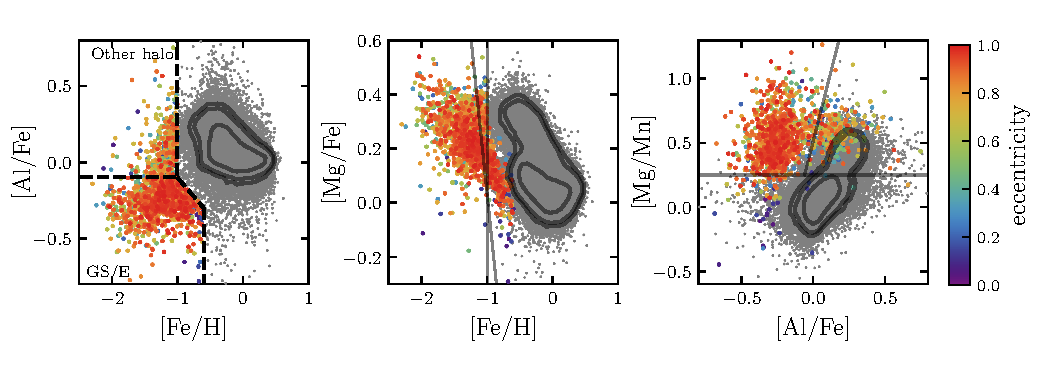
\includegraphics[width=\textwidth]{figure/ch3/halo_abundances.pdf}
    \caption{Abundances of the stellar sample: [Al/Fe] versus [Fe/H] (\textit{left}), [Mg/Fe] versus [Fe/H] (\textit{middle}), and [Mg/Mn] versus [Al/Fe] (\textit{right}). Coloured points show stars from the halo sample, selected chemically by their [Fe/H] and [Al/Fe] abundances. The dashed lines in the left panel show the selection used to pick these stars. Points are coloured by their eccentricity. Grey points are stars from the quality sample not chosen to be part of the halo. The thin solid lines in the middle and right panels show reference lines and selections from the literature (see text).}
    \label{ch3:fig:halo_abundances}
\end{figure}

% Kinematic subsample
From the halo sample, we identify a subset of likely members of the GS/E remnant following the recommendations and approach of \cite{lane22}. Those authors built DF-based models of the nearby Milky Way stellar halo using the anisotropy parameter $\beta$ as a proxy for the two major stellar halo populations: $\beta=0.9$ for the high-[Fe/H], radially anisotropic GS/E remnant, and $\beta=0.5$ for the low-[Fe/H], more isotropic traditional stellar halo. Using these models, \cite{lane22} identified regions of various kinematic spaces where stars from the high-$\beta$ component were found with low contamination from the low-$\beta$ component. The `best' kinematic spaces were those where purity was around $\sim 0.8$, and these included \eLz, the action diamond, and \JRLz. We use the elliptical selection criteria from table~2 (The \textit{Survey} selections) of \cite{lane22}, defining a separate GS/E subsample for each of these three kinematic spaces. Figure~\ref{ch3:fig:halo_kinematics} shows these three spaces, the GS/E selections, as well as the chemically selected halo sample coloured by [Fe/H]. Our GS/E subsamples defined using the \eLz\ plane, action diamond, and \JRLz\ plane contain 163, 77, and 319 stars respectively.

\begin{figure}
    \centering
    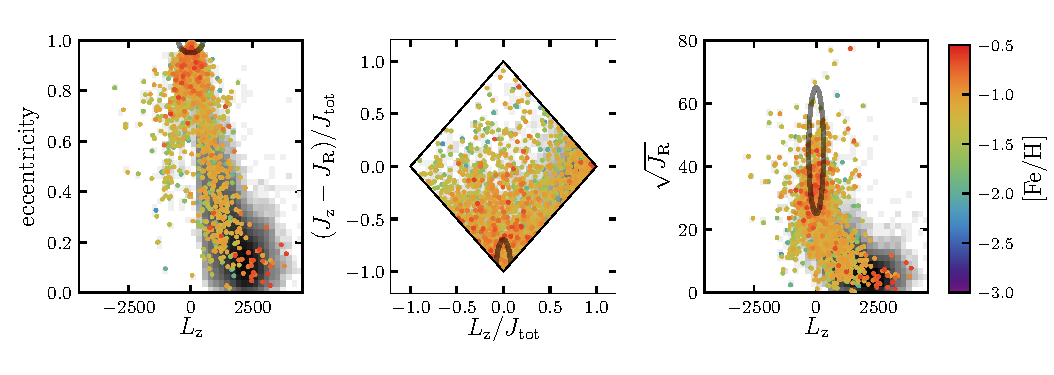
\includegraphics[width=\textwidth]{figure/ch3/halo_kinematics.pdf}
    \caption{Kinematics of the chemically selected halo sample. Points are coloured by their [Fe/H] abundances. The thin black lines show the kinematic selections used to define the high-purity GS/E subsamples based on \cite{lane22}. The background histogram shows stars from the high-quality sample not chosen to be part of the halo.}
    \label{ch3:fig:halo_kinematics}
\end{figure}

% Issues that we will return to
We consider three kinematic spaces here so that we may examine the differences in outcomes of our model-fitting procedure. This type of selection constitutes a significant bias when modelling GS/E, in so far as we discount a large fraction of stars belonging to the high-$\beta$ GS/E population where they overlap with the low-$\beta$ halo. To wit, completeness for these selections is typically between $0.3-0.7$ and, as we shall show, is spatially non-trivial. We return to these DF-based models in \S~\ref{ch3:subsec:kinematic-effective-selection-function} when we discuss the creation of the kinematic effective selection function which addresses these biases in the density modelling framework.

% Thick disk contamination
The final step in cultivating our subsamples of GS/E stars for modelling is to address contamination from thick disk populations. \cite{lane22} include a thin and thick disk component in their models, but acknowledge that this simplifies the complicated underlying nature of the Milky Way disk, which is closer to a continuum of disk populations parametrized by scale height, length, and velocity dispersion \parencite{bovy12d}. The selections of \cite{lane22} find near-perfect separation between thick disk and high-$\beta$ populations, but their simple model is unable to account for the kinematically hottest thick disk populations. Even though these populations are numerically insignificant in the context of the density of the stellar disk, they are significant in the context of the density of the stellar halo.

% Using abundances
Fortunately, these populations should be somewhat distinct in abundance space. Figure~\ref{ch3:fig:selection_abundances} shows the GS/E subsamples in [Fe/H] versus [Al/Fe] (top row) and [Mg/Fe] (bottom row). Since \textit{in-situ} populations (both disk and stellar halo) should occupy the higher [Al/Fe] portion of our halo selection region, we make a cut at [Al/Fe] $= -0.1$ and only consider kinematically selected stars with lower [Al/Fe] to be part of our GS/E subsamples. In Figure~\ref{ch3:fig:selection_abundances}, the horizontal dashed line is set at [Al/Fe] $= -0.1$, and stars with greater [Al/Fe] abundances are shown as black crosses in both sets of panels. In [Fe/H] versus [Mg/Fe], many of the stars which are discounted occupy the high-[Mg/Fe], intermediate-[Fe/H] part of the distribution, exactly where thick disk and \textit{in-situ} halo would expect to be found. We are therefore confident that this cut serves only to enhance the purity of our GS/E subsamples and does not confer any bias. The fraction of stars removed is 5--8~per~cent of the sample depending on the kinematic space. The final GS/E subsamples defined by the kinematic selections, including this cut in [Al/Fe] contain 151 (\eLz), 73 (AD), and 300 (\JRLz) stars.

% Marginalized abundances
The top and two rightmost panels in Figure~\ref{ch3:fig:selection_abundances} show the marginalized [Fe/H], [Al/Fe] and [Mg/Fe] abundance distributions respectively. The coloured lines are Gaussian kernel density estimates for each of the three kinematic selections and the grey line shows the same for the whole sample. Dashed lines show the medians in the same colours, which are all similar, deviating by no more than 0.02 dex for each abundance. These medians are approximately -1.17, -0.23, and 0.20 for [Fe/H], [Al/Fe], and [Mg/Fe] respectively.

\begin{figure}
    \centering
    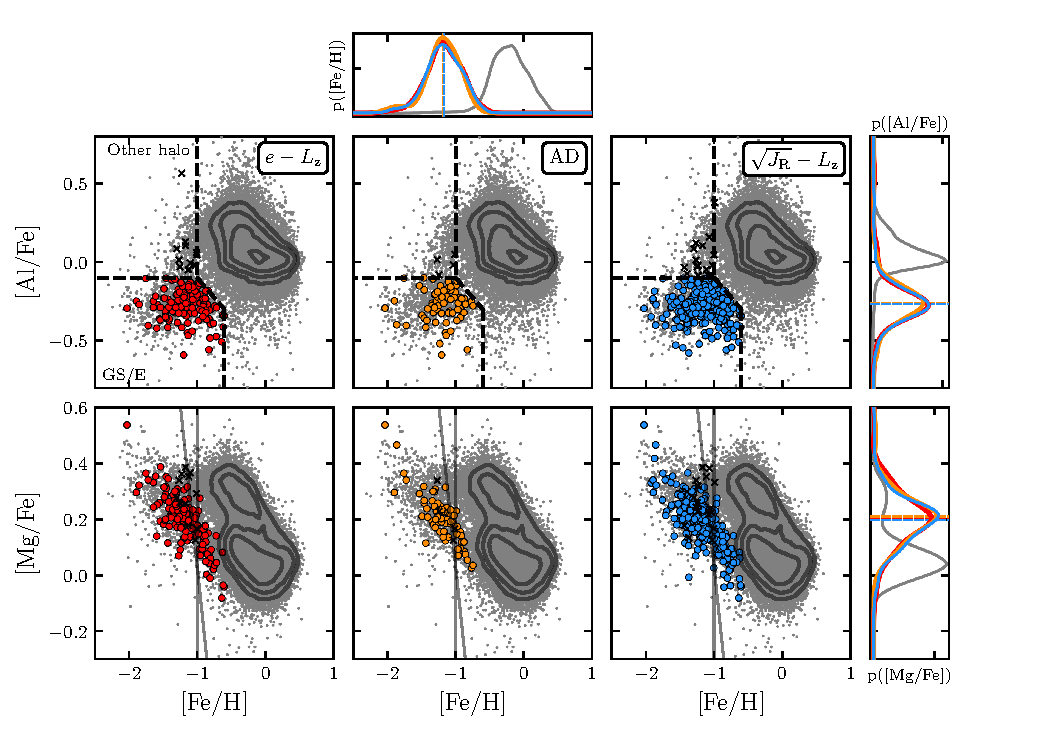
\includegraphics[width=\textwidth]{figure/ch3/kinematic_sample_abundances.pdf}
    \caption{Abundances of the kinematically selected GS/E subsamples: [Al/Fe] versus [Fe/H] (\textit{top}) and [Mg/Fe] versus [Fe/H] (\textit{bottom}). Each column shows a high-purity GS/E subset of the stars from the halo sample chosen using one of the kinematic selections (labelled). The solid and dashed are the same as described in Figure~\ref{ch3:fig:halo_abundances}. The points which have [Al/Fe] $< -0.1$ are deemed to be accreted stars, and therefore part of the GS/E subsamples, and are shown with coloured points in both top and bottom panels. The points with [Al/Fe] $> -0.1$ are deemed to be \textit{in-situ} stars, not part of the GS/E subsamples, and are shown with black crosses. The top-most panel shows the marginalized [Fe/H] abundance for all stars (grey), as well as each of the three kinematic samples (coloured according to the main panels in the figure). The lines in this margin are Gaussian kernel density estimates. The dashed lines show the medians of the samples. The two right-most panels show the margins for [Al/Fe] and [Mg/Fe] constructed in the same way.}
    \label{ch3:fig:selection_abundances}
\end{figure}

\section{Method}
\label{ch3:sec:method}

In this section we describe our approach to modelling the density of both the whole stellar halo and the GS/E subsamples. We describe the manner in which we account for the biases imposed on our samples by the APOGEE selection function and by the high-purity GS/E kinematic selections. We then outline how density profiles are normalized and total masses are derived. Finally, we demonstrate that our technique is robust and yields accurate results by applying it to mock data.

\subsection{Density Modelling}

We fit density profiles to both our halo and GS/E samples, accounting for the survey selection function, dust extinction, and the colour-magnitude density of the tracer population. We generally follow the well-established approach presented by \textcite{bovy12d} (also discussed by \textcite{rix13}), and then built upon and used more recently by \textcite{bovy16a,bovy16b,mackereth17,horta21b} and \cite{mackereth20}. We describe here the method in broad detail, and encourage the reader to refer specifically to \textcite{bovy12d,bovy16a} and \cite{mackereth20} for more information.

We model the observed APOGEE star counts as a Poisson point process, with rate function $\lambda(O \vert \Theta)$. Here, the data $O \equiv [\ell, b, D, \mu_{[\ell,b]}, v_\mathrm{LOS}, H, (J-K_\mathrm{S})_{0}, [\mathrm{Fe/H}]]$ are the Galactic coordinates $\ell$ and $b$, heliocentric distance $D$, proper motions in Galactic coordinates $\mu_{[\ell,b]}$, the heliocentric line-of-sight velocity $v_\mathrm{LOS}$, the apparent $H$-band magnitude $H$, the dereddened colour $(J-K_\mathrm{S})_{0}$, and the iron abundance [Fe/H]. The vector $\Theta$ of parameters describes the density profile under consideration and is to be determined by fitting to the data. The rate function can be expressed as

\begin{equation}
\label{ch3:eq:rate}
\begin{split}
	\lambda(O \vert \Theta) & = \nu_{\star}(\vec{X} \vert \Theta) \times f(\vec{v} \vert \vec{X}) \\
	& \times \vert J(\vec{X}, \vec{v}; \ell, b, D, \mu_{[\ell,b]}, v_\mathrm{LOS}) \vert \\
	& \times \rho(H, (J-K_\mathrm{S})_{0}, [\mathrm{Fe/H}] \vert \vec{X}) \\
	& \times S(\ell, b, D, \mu_{[\ell,b]}, v_\mathrm{LOS}, H, (J-K_\mathrm{S})_{0})
\end{split}
\end{equation}

\noindent where $\nu_{\star}(\vec{X} \vert \Theta)$ is the stellar number density as a function of rectangular Galactocentric coordinates $\vec{X}$ and $f(\vec{v} \vert \vec{X})$ is the velocity distribution function to which we will return in the next section when we come to the kinematic selection function. While the velocity DF in general depends on parameters $\Theta$ fit to the data, here we use a fixed velocity DF $f(\vec{v}\vert \vec{X})$ to keep the fit computationally tractable. We address the implication of this choice later in the discussion. The function $\rho(H, (J-K_\mathrm{S})_{0}, [\mathrm{Fe/H}] \vert \vec{X})$ is the apparent density of stars in colour, magnitude, and abundance space for a given position. $\vert J(\vec{X}, \vec{v}; \ell, b, D, \mu_{[\ell,b]}, v_\mathrm{LOS}) \vert$ is the Jacobian linking observed coordinates with Galactocentric coordinates, which may be split into a spatial and velocity component as $\vert J_{1}(\vec{X}; \ell, b, D) J_{2}( \vec{v}; \ell, b, D \mu_{[\ell,b]}, v_\mathrm{LOS}) \vert$. Finally, $S(\ell, b, D, \mu_{[\ell,b]}, v_\mathrm{LOS}, H, (J-K_\mathrm{S})_{0})$ is the selection function, which depends on sky location, heliocentric distance, velocity, as well as colour and magnitude. This single selection function can be separated into a spatial component, $S_{1}$, and a kinematic component, $S_{2}$, as $S(\ell, b, D, \mu_{[\ell,b]}, v_\mathrm{LOS}, H, (J-K_{\mathrm{S}0}) = S_{1}(\ell, b, H, (J-K_\mathrm{S})_{0}) \times S_{2}(\ell, b, D, \mu_{[\ell,b]}, v_\mathrm{LOS})$. The spatial component arises from the APOGEE targeting procedure, which has been briefly discussed in \S~\ref{ch3:sec:data}. This function describes the probability with which a star with a given $H$-band magnitude and $(J-K_\mathrm{S})_{0}$ colour will be included for observation in the APOGEE statistical sample, and varies based on field. We follow the approach of \cite{mackereth20} when constructing $S_{1}$, and details may be found in their Appendix~A. The kinematic component of the selection function arises from our selection of GS/E stars, and its construction will be described below.

As in \textcite{bovy12d}, the log likelihood of the model parameters may be written in terms of the rate function as

\begin{equation}
\label{ch3:eq:log-likelihood}
	\ln \mathcal{L}(\Theta) = \sum_{i} \big[ \ln \nu_{\star}(\vec{X}_{i} \vert \Theta) - \ln \int \mathrm{d}O\ \lambda(O \vert \Theta) \big].
\end{equation}

\noindent Derivation of this likelihood uses the fact that the rate function only depends on $\Theta$ through $\nu_{\star}(\vec{X} \vert \Theta)$, because as we discussed above, the velocity DF does not depend on parameters that we fit. If the velocity DF were to depend on $\Theta$ as well, the first term would simply be $\ln [\nu_{\star}(\vec{X}_{i} \vert \Theta)\,f(\vec{v}_{i} \vert \vec{X}_i,\Theta)]$. The integral in the likelihood equation is the effective volume, which expresses for a given set of model parameters the expected (non-normalized) number of stars. For APOGEE, the effective volume can be expressed as 

\begin{equation}
\label{ch3:eq:effective-volume}
\begin{split}
	\int \mathrm{d}O \lambda(O \vert \Theta) = \sum_\mathrm{fields} \Omega_\mathrm{field} \int & \mathrm{d}D\ D^{2} \nu_{\star} (\vec{X}(\mathrm{field},D) \vert \Theta) \\
	\times & \mathfrak{S}_{1}(\mathrm{field},D) \times \mathfrak{S}_{2}(\mathrm{field},D).
\end{split}
\end{equation}

\noindent Here, the effective volume is a sum over each APOGEE field of area $\Omega_\mathrm{field}$ under consideration. This is permitted for a survey such as APOGEE which is comprised of a number of small ($< 2$~degree size), non-overlapping fields, since we can assume that the density is constant across the angular extent of each field (an assumption which we test, finding it to be valid at level of about 1~per~cent). Recall in \S~\ref{ch3:subsec:observations} we removed any APOGEE field with noticeable contamination from a globular cluster, which helps to enforce this assumption. In the integral the density is as above, but the positions $\vec{X}$ are evaluated along the line-of-sight of each field. $\mathfrak{S}_{1}$ and $\mathfrak{S}_{2}$ are the spatial and kinematic \textit{effective selection functions}. Similar to $S_{1}$ and $S_{2}$, the effective selection functions include additional information required for the modelling procedure, yet which is independent of the model parameters of interest $\Theta$. 

The spatial effective selection function $\mathfrak{S}_{1}$ is determined by marginalizing $S_{1}$ over the colour, absolute magnitude, and metallicity distribution of the tracer population, including the effects of dust obscuration. It is given by

\begin{equation}
\label{ch3:eq:effective-selection-function}
\begin{split}
\mathfrak{S}_{1}(\mathrm{field},D) = \iiint & \mathrm{d} M_{H}\ \mathrm{d} (J-K_\mathrm{S})_{0}\ \mathrm{d} [\mathrm{Fe/H}] \\
& \times S_{1}(\mathrm{field}, M_{H}+\mu(D), (J-K_\mathrm{S})_{0}]) \\
& \times \rho(M_{H},(J-K_\mathrm{S})_{0}, [\mathrm{Fe/H}]) \\
& \times \frac{\Omega_{j}(H_{[\mathrm{min},\mathrm{max}],j},M_{H},A_{H}(\ell,b,D),D)}{\Omega_\mathrm{field}}.
\end{split}
\end{equation}

Here $\rho(M_{H},(J-K_\mathrm{S})_{0},[\mathrm{Fe/H}])$ and $S_{1}(\mathrm{field}, H, (J-K_\mathrm{S})_{0})$ are as above. We have introduced the absolute magnitude $M_{H} = H - \mu(D)$, which relates to the apparent magnitude by the distance modulus $\mu(D)$, and is the preferred quantity for this integration. In the main APOGEE survey each field is divided up into $j$ bins of apparent ${H}$-band magnitude and $(J-K_\mathrm{S})_{0}$, which are each bounded by a minimum and maximum magnitude $H_{[\mathrm{min},\mathrm{max}]}$. The factor $\Omega_{j}/\Omega_\mathrm{field}$ is the fraction of observable area of the plate given the local extinction and the limiting $H$-band magnitudes for each bin. $\Omega_\mathrm{field}$ is the total area of each plate, and $\Omega_{j}$ is given by

\begin{equation}
\begin{split}
& \Omega_{j}(H_{[\mathrm{min},\mathrm{max}],j},M_{H},A_{H}(\ell,b,D),D) = \\
& \Omega(H_{\mathrm{min},j} < M_{H}+\mu(D)+A_{H}(\ell,b,D) < H_{\mathrm{max},j} )
% & \Omega(H_{\mathrm{min},j} - [M_{H}+\mu(D)] < A_{H}(\ell,b,D) < H_{\mathrm{max},j} - [M_{H}+\mu(D)] )
\end{split}
\end{equation}

\noindent where $A_{H}(\ell,b,D)$ is the $H$-band extinction. Intuitively, as extinction increases stars may be extinguished into or out of a given colour-magnitude bin, and the factor $\Omega_{j}$ expresses this effect. Note that since $(J-K_\mathrm{S})_{0}$ is the dereddened colour we assume it is not impacted by extinction and so does not appear in the definition of $\Omega_{j}$. The $H$-band extinction is obtained from the dust map of \textcite{bovy16a}, which is a combination of the dust maps from \textcite{marshall06}, \textcite{green15}, and \textcite{drimmel03}. We query this dust map using the \texttt{mwdust} python package\footnote{\url{https://github.com/jobovy/mwdust}}.

In practice, this spatial effective selection function integral is approximated by Monte Carlo sampling the distribution of colours, absolute magnitudes, and iron abundances of the red giant tracer population. These distributions are sourced from a grid of PARSEC v1.2S isochrones \parencite{bressan12}. The grid is spaced linearly in metal fraction with $\Delta \mathrm{Z} = 0.0001$ and a minimum [Fe/H] of -3. The ages of the grid span $10-14$~Gyr, with the minimum age being appropriate for GS/E \parencite{montalban21}. We draw samples from regions of the isochrone grid bounded by $1 < \log g < 3$ weighted by a \textcite{chabrier03} initial mass function. The contributions from each isochrone are weighted such that the samples are spaced linearly in [Fe/H] and linearly in age. When fitting the whole-halo sample we use a [Fe/H] range of [-3,-0.6], and when fitting the GS/E subsamples we use a slightly more metal-rich range: [-2,-0.6] to reflect approximate spread in [Fe/H] observed for GS/E \parencite[see our Figure~\ref{ch3:fig:selection_abundances} or refer to e.g.][]{myeong19,hasselquist21,horta23a}. Otherwise, the fits to the halo and GS/E samples both use the same isochrone grid. The effective selection function is calculated on a grid for each APOGEE field with 300 bins between $7 < \mu(D) < 19$ (roughly $0.25~\mathrm{kpc} < D < 65~\mathrm{kpc}$) spaced linearly in distance modulus.

\subsection{The Kinematic Effective Selection Function}
\label{ch3:subsec:kinematic-effective-selection-function}

The kinematic effective selection function can be expressed as:

\begin{equation}
\label{ch3:eq:kinematic-effective-selection-function}
\begin{split}
    \mathfrak{S}_{2}(\mathrm{field},D) = \int & \mathrm{d} \vec{v}\ f(\vec{v} \vert \vec{X}(\ell, b, D)) \\
    & \times \lvert J_{2}(\vec{v}; \ell, b, D, \mu_{[\ell,b]}, v_{\mathrm{LOS}}) \rvert \\
    & \times S_{2}(\ell, b, D, \mu_{[\ell,b]}, v_{\mathrm{LOS}})
\end{split}
\end{equation}

where $f$, $J_{2}$, and $S_{2}$ are all as above, but defined at field locations $(\ell,b,D)$. As discussed by \cite{mackereth20}, the ideal approach for handling stellar kinematics is to have a parametrized DF $f(\vec{v} \vert \vec{X}, \Theta)$ which may be used to kinematically select populations with a set of rules $S_{2}$. The downside of this approach is twofold: first, DFs -- particularly realistic ones -- tend to be computationally expensive to compute, and second, this expands the coordinate space to 6D. These two effects combine such that it is impractical to use DFs with varying parameters which must be integrated on the fly during the optimization of the likelihood.

\cite{mackereth20} bypassed this issue by asserting that the two major halo stellar populations: the radially anisotropic, high-[Fe/H] GS/E remnant, and the more isotropic, low-[Fe/H] traditional stellar halo are well-separated by eccentricity. In this work, we adopt a more sophisticated approach, leveraging the DF-based models of \cite{lane22}, which we have already discussed in the context of GS/E sample selection. We will use this model to construct the kinematic effective selection function in such a way that it is independent of any model parameters $\Theta$.

To briefly summarize the model of \cite{lane22}, they consider anisotropic distribution functions of the form \parencite[see, e.g.][]{binney08}

\begin{equation}
    \label{ch3:eq:anisotropic-df}
    f(\mathcal{E},L) = L^{-2\beta}f_{1}(\mathcal{E}).
\end{equation}

Here, $\mathcal{E} = \Psi - \frac{1}{2}v^{2}$ is the binding energy and $\Psi = -\Phi + \Phi_{0}$ is the negative of the gravitational potential normalized such that $\Psi(\infty) = 0$. $L$ is the total angular momentum, $v$ is the velocity magnitude, and $\beta$ is the anisotropy parameter, defined as

\begin{equation}
    \label{ch3:eq:beta}
    \beta = 1- \frac{\sigma_{T}^{2}}{2\sigma^{2}_{r}}\,,
\end{equation}

\noindent where $\sigma_{T}$ is the quadrature sum of the azimuthal and polar velocity dispersions, and $\sigma_{r}$ is the velocity dispersion in the radial direction. The function $f_{1}$ relates the mass density of the DF to the underlying potential and is, in general, non-trivial to compute, often requiring solving multiple integrals numerically \parencite[For more information see ][ particularly Appendix A]{lane22}.

We use the same underlying potential \parencite[\texttt{MWPotential2014 of }][]{bovy15} and mass density for the DF as \cite{lane22}. The mass density is a spherical truncated power law with power law index $\alpha=3.5$ and truncation radius $r_{c} = 25$~kpc, taken from the stellar halo fits of \cite{mackereth20}. We use $\beta=0.3$ to represent the low-[Fe/H] traditional stellar halo, and $\beta=0.8$ to represent the high-[Fe/H] GS/E halo. We modify our choice of high- and low-$\beta$ compared with \cite{lane22}, who use $\beta=0.9$ and $\beta=0.5$. A smaller value for the low-$\beta$ component aligns slightly better with the accepted values for the metal-poor halo from the literature \parencite{belokurov18,fattahi19,lancaster19,iorio21}. With regards to the anisotropy of the high-$\beta$ component, the literature does support a value of $\beta \sim 0.9$ \parencite{belokurov18,fattahi19,lancaster19,iorio21}, However we prefer to be conservative with our choice of $\beta=0.8$ since \cite{lane22} did note some minor numerical issues when using DFs with higher values of $\beta$. Additionally, as we shall show, by modelling GS/E with $\beta=0.8$ we are actually constructing an upper limit on the mass when compared with a mass derived using a higher value of $\beta$.

 We set these two components to have equal density in our models in order to enforce the assumption that the two components exist in roughly equal density near the position of the Sun. While it may seem odd that we are fixing the parameters of the mass density distribution of the stellar halo in our DF models before setting out to use them to measure the mass density distribution of the stellar halo, we are confident of a scheme to ensure that this does not significantly bias our results, and will discuss more in \S~\ref{ch3:sec:discussion}. It is worthwhile to note though that only the high-$\beta$ component is relevant for calculating the kinematic effective selection function, the low-$\beta$ component is only used to estimate purity, which is simply informative. Additionally, the overall normalization of this high-$\beta$ DF is also unimportant, only its shape, which is determined by the value of $\beta$ as well as the form of the underlying density profile. These two factors contribute to the reasoning why the kinematic effective selection function is resilient to changes in the assumptions of our models, which we will expand upon later.

\cite{lane22} studied samples drawn from these DFs at positions where APOGEE had observed stars. We adopt a similar approach when computing $\mathfrak{S}_{2}(\mathrm{field},D)$. At each location where we calculate $\mathfrak{S}_{2}$, we draw $10^{3}$ velocity samples from our DFs and calculate actions and eccentricities in a manner identical to that used for our stellar samples (\S~\ref{ch3:sec:data}). We then calculate the completeness of the high-$\beta$ component given each of the kinematic selections used in \S~\ref{ch3:subsec:halo-gse-samples} (i.e., the fraction of high-$\beta$ samples lying in the selection compared with the total number of high-$\beta$ samples), which is equivalent the value of $\mathfrak{S}_{2}$. Drawing samples from DFs and calculating kinematic quantities is computationally expensive, and so rather than compute $\mathfrak{S}_{2}$ for each point on a grid identically to the grid on which we computed $\mathfrak{S}_{1}$, we compute it only for 21 points, evenly spanning the same range of distance modulus (7 to 19), for each field. We then linearly interpolate the value of $\mathfrak{S}_{2}$ between these 21 points when combining it with the more densely sampled $\mathfrak{S}_{1}$. 

Figure~\ref{ch3:fig:ksf_dmod_fields} shows the value of $\mathfrak{S}_{2}$ as a function of distance modulus for each of the three kinematic selections. Each field is shown as a different line, coloured by the absolute value of the Galactic latitude of its on-sky location. Only fields with stars included in the halo sample are shown. In a smaller panel at the top of the figure we show the distribution of distance moduli of our halo sample for reference. The value of $\mathfrak{S}_{2}$ fluctuates along a field due to the finite number of samples drawn at each location, but this noise clearly averages out in the agregate of many fields. Figure~\ref{ch3:fig:ksf_lb_dmod_marginalized} shows the value of $\mathfrak{S}_{2}$ marginalized along each line of sight using a spline fit to the distribution of distance moduli in the top panel of Figure~\ref{ch3:fig:ksf_dmod_fields} (red line) as a function of Galactic coordinates. Again, only fields which have stars in the halo sample are shown, and the $20\degr$ box we use to exclude bulge fields is shown. 


\begin{figure}
    \centering
    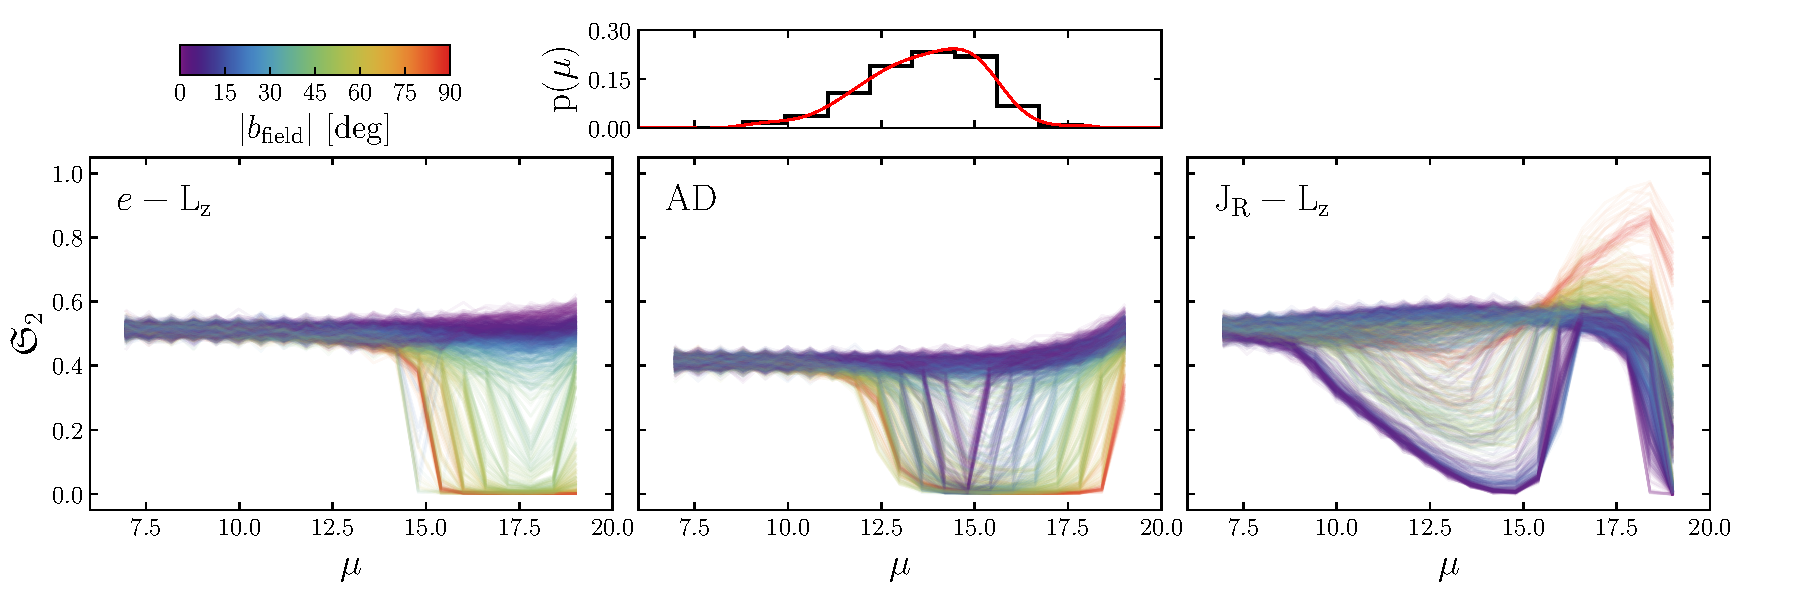
\includegraphics[width=\textwidth]{figure/ch3/ksf_dmod_fields.pdf}
    \caption{Kinematic effective selection function shown versus distance modulus, $\mu$, for each line of sight in APOGEE. Each of the large panels shows the kinematic effective selection function derived using a different set of kinematic parameters (labelled) and its corresponding selection criterion (see \S~\ref{ch3:subsec:halo-gse-samples}). The colour of the individual lines shows the absolute value of the Galactic latitude of the field coordinates. The small top panel shows the distribution of distance modulus for the halo subsample, and the red line shows the cubic spline fit to the distribution, which is used to marginalize $\mathfrak{S}_\mathrm{2}$ along the line of sight in Figure~\ref{ch3:fig:ksf_lb_dmod_marginalized}.}
    \label{ch3:fig:ksf_dmod_fields}
\end{figure}

\begin{figure}
    \centering
    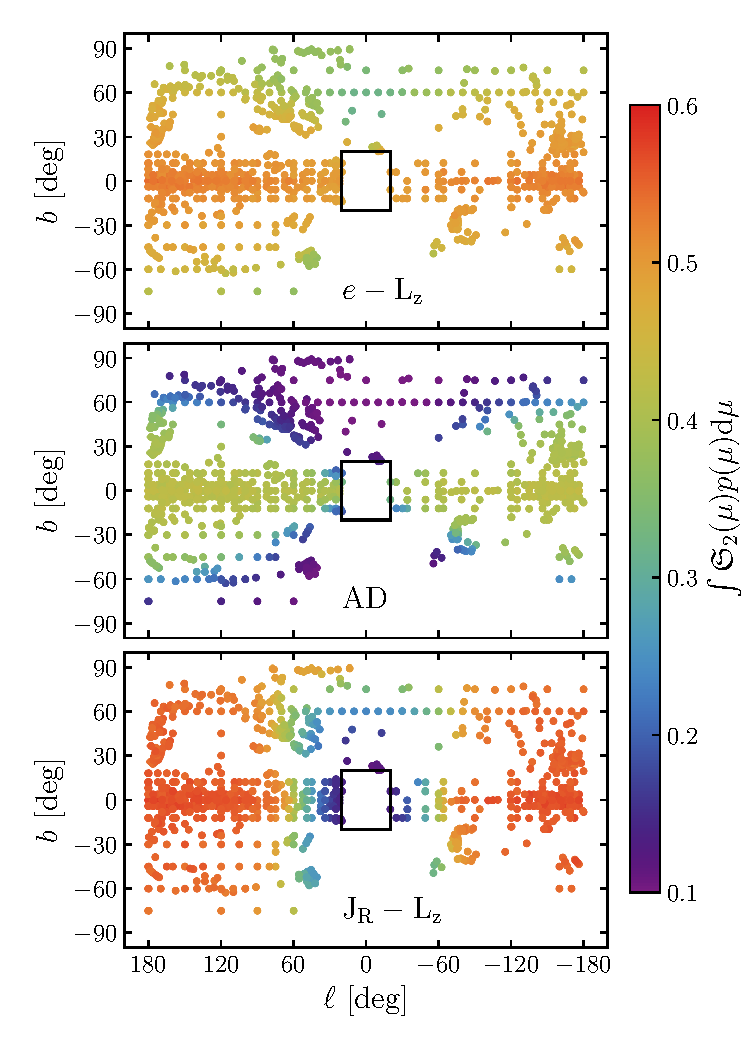
\includegraphics[width=0.7\textwidth]{figure/ch3/ksf_lb_dmod_marginalized.pdf}
    \caption{The kinematic effective selection function, $\mathfrak{S}_\mathrm{2}$, marginalized over the distance modulus distribution of sources (see Figure~\ref{ch3:fig:ksf_dmod_fields}) for each line of sight shown in Galactic coordinates. The three panels show three kinematic spaces used to produce the kinematic effective selection functions (labelled).}
    \label{ch3:fig:ksf_lb_dmod_marginalized}
\end{figure}

These two figures each reveal an interesting perspective of $\mathfrak{S}_{2}$. Figure~\ref{ch3:fig:ksf_dmod_fields} shows how it can vary along each line of sight, and similarly Figure~\ref{ch3:fig:ksf_lb_dmod_marginalized} shows how it can vary as a function of sky coordinates. These variations are principally due to the change in kinematics as a function of radius, which when mapped into a heliocentric frame and weighted by the distribution of halo star distance moduli yields interesting patterns. A secondary effect is that samples drawn near the Galactic poles will behave differently than those at a similar radius in the plane. Directly above the centre of the Galaxy, the St\"{a}eckel approximation is a poor one, impacting actions and eccentricities, and also the kinematic selections are ill-suited to describe the distributions which arise. While this effect is somewhat pathological, it is at least entirely self-consistent within the modelling framework, such that the data and $\mathfrak{S}_{2}$ are impacted in the same way. This gives rise to the general trend of worsening $\mathfrak{S}_{2}$ with larger absolute Galactic latitude seen in both Figure~\ref{ch3:fig:ksf_dmod_fields} and \ref{ch3:fig:ksf_lb_dmod_marginalized}. For both \eLz\ and AD, $\mathfrak{S}_{2}$ is reasonably constant at distances characteristic of our sample ($\mu \sim 10-17$), with the decreases in $\mathfrak{S}_{2}$ associated with Galactocentric radius and latitude occuring at slightly lower $\mu$ for the AD space. On the other hand, $\mathfrak{S}_{2}$ has a much more complicated behaviour on a field-by-field basis for \JRLz. 

\subsection{Stellar number density models}
\label{ch3:subsec:density-models}

We consider several models for the stellar number density, which will be fit both to the whole stellar halo sample and the GS/E subsamples. We follow the approach of \cite{mackereth20} in our construction of these density profiles, which are general and flexible. All of our models are triaxial and expressed as functions of an effective radius.

\begin{equation}
\label{ch3:eq:effective-radius}
m = \sqrt{ X^{\prime^{2}} + \frac{Y^{\prime^{2}}}{p^{2}} + \frac{Z^{\prime^{2}}}{q^{2}} }
\end{equation}

\noindent where $[X,Y,Z]^{\prime}$ are rectangular coordinates in the rotated frame. $p$ is the ratio of the $Y^{\prime}$ to $X^{\prime}$ axes, and $q$ is the ratio of the $Z^{\prime}$ to $X^{\prime}$ axes. Each model has a flexible orientation parametrized by three variables: $\theta$, $\eta$, and $\phi$. First, the density profile is rotated in the $X^{\prime}-Y^{\prime}$ plane clockwise by an angle $\phi$, then the $Z^{\prime}$ axis is rotated towards a unit vector $\hat{z} = \big[ \sqrt{ 1-\eta^{2} } \cos\theta, \sqrt{ 1-\eta^{2} } \sin\theta, \eta \  \big]$. So the parameter $\theta$ controls the angle of the transformed $Z^{\prime}$-axis of the ellipsoid (i.e., the axis of the ellipsoid originally aligned with the $Z^{\prime}$ axis) in the plane of the Galaxy, and $\eta$ controls the degree to which the transformed $Z^{\prime}$-axis is oriented towards the Galactic north pole. Even sampling of these three parameters evenly samples the unit sphere. 

The density profiles we consider are as follows. The first is a simple power law profile

\begin{equation}
\label{ch3:eq:single-power-law}
\nu_{\star} \propto m^{-\alpha_{1}}
\end{equation}

\noindent where $\alpha_{1}$ is the power-law index. The second is a single power-law profile with an exponential truncation scale $r_{c}$, which is expressed as 

\begin{equation}
\label{ch3:eq:exp-truncated-power-law}
\nu_{\star} \propto m^{-\alpha} \exp(-m/r_{c}) .
\end{equation}

\noindent Finally, we have broken power law models with two or three break radii which take the form

\begin{equation}
\label{ch3:eq:broken-power-law}
\nu_{\star} \propto 
\begin{cases}
m^{-\alpha_{1}} & ; m \leq r_{1} \\
r_{1}^{\alpha_{2}-\alpha_{1}} m^{-\alpha_{2}} & ; r_{1} < m \leq r_{2} \\
r_{2}^{\alpha_{3}-\alpha_{2}} m^{-\alpha_{3}} & ; r_{2} < m
\end{cases}
\end{equation}


\noindent where $r_\mathrm{i}$ are the break radii (we use $r$ to emphasize that these are radii), and $\alpha_\mathrm{i}$ are the power law indices. Together these four models span a range of complexity, and are similar to others used in the literature. Throughout the rest of the paper we refer to the single power law model as `SPL', the exponentially truncated single power law model as `SC', and the broken power law models with one or two breaks as `BPL' and `DBPL', respectively.

Each of these models is considered on its own, but also with a disk contamination model. While we are confident that we have removed most of the disk contamination using abundance cuts, we recognize that some contamination is unavoidable. The disk contamination model is exponential, with radial scale length 2.2~kpc and vertical scale length 0.8~kpc \parencite{mackereth17}. We parametrize contamination by including a factor $f_\mathrm{disk}$ which expresses the fraction of density at the solar position contributed by the disk model. The combined model takes the form

\begin{equation}
\label{ch3:eq:disk-contamination}
\nu_{\star} (m) \propto (1-f_\mathrm{disk}) \nu_{\star,\mathrm{halo}}(m) + f_\mathrm{disk} \nu_{\star,\mathrm{disk}}(m) .
\end{equation}

\noindent Models including disk contamination are referred to with `+D' after the shorthand introduced above (i.e. `SPL+D').

In fitting these models, power law indices are allowed to take any value and are nominally positive (indicating decreasing density), but occasionally the exponentially truncated models have negative $\alpha$. Indices are also required to steepen in broken power law models such that $\alpha_{1} < \alpha_{2} < \alpha_{3}$. Truncation radii for both exponentially truncated and broken power laws are required to lie in the range $[2,55]$~kpc. The inner range is motivated by the fact that we exclude any fields within a $20\degr$ box around the bulge ($20\degr$ at $\sim 8$~kpc is $\sim 2$~kpc). The outer range is driven by the fact that the effective selection function essentially becomes zero for all fields at this distance. Even though our most distant star lies at nearly 40~kpc, our statistical leverage extends to the point at which the effective selection function is zero, which is about 55~kpc. The shape parameters $p$ and $q$ are defined on the interval $(0,1]$ such that the axis of the ellipsoid aligned with the $X^{\prime}$ axis (rotated frame) is always the longest. Of the orientation parameters, $\theta$ can take values between $[0,2\pi]$, $\eta$ can take values between $[0.5,1]$, and $\phi$ is defined between $[0,\pi]$. $\eta$ and $\phi$ could take wider ranges but these are degenerate with other combinations of orientation parameters as well as $p$ and $q$. Finally, the disk contamination parameter $f_\mathrm{disk}$ is defined on the interval $[0,1]$.

\subsection{Fitting density models}
\label{ch3:subsec:fitting-density-models}

To find the best-fitting set of parameters for each model, we use Markov Chain Monte Carlo to sample the posterior of the likelihood \eqref{ch3:eq:log-likelihood}. We use the affine-invariant ensemble sampler of \textcite{goodman10} implemented in \texttt{emcee} \parencite{foreman-mackey13}. We first optimize the likelihood function using Powell's method \parencite{powell64} and then initialize one hundred walkers with a small amount of noise around that set of optimized parameters. Each walker moves $10^{4}$ steps and we remove the first $10^{3}$ steps as burn-in. We define the best-fitting parameters as the median of this set of posterior samples, with the uncertainty being the 16th and 84th percentiles. Our posteriors are complicated, however, and while we explored other more sophisticated methods of determining the best-fitting parameters and uncertainties we defer back to this approach for its simplicity. For this reason, we make our chains available online \footnote{\url{https://doi.org/10.5281/zenodo.8339417}}.

\subsection{The mass from normalization of the amplitude of the density function}
\label{ch3:subsec:mass-calculation-from-normalization}

To determine the mass of each density profile and its array of parameter samples drawn from the posterior, we follow the approach of \cite{mackereth20} which we describe here briefly. First, we normalize the density profiles from \S~\ref{ch3:subsec:density-models} and then integrate the density profiles over a range of Galactocentric radii. With regards to normalization, each density profile is fit such that the density is 1 at the solar position: $\nu_{\star}(\vec{X}_{\odot}) = 1$. The number of stars expected for a given density profile and parameter vector $\Theta$ is therefore the rate function of equation~\eqref{ch3:eq:rate}, which is the product of the density and the effective selection functions, integrated over the volume of the survey. This quantity is identical to the effective volume expressed in equation~\eqref{ch3:eq:effective-volume}. Dividing the total number of observed APOGEE stars to which the density profile is fit, $N_{\mathrm{obs}}$, by this expected number of stars given $\nu_{\star}(\vec{X}_{\odot}) = 1$ gives the proper normalization of the density profile in units of observed APOGEE red giants per volume, and is expressed as

\begin{equation}
\label{ch3:eq:density-normalization}
A(\Theta) = \frac{ N_\mathrm{obs} }{ \int \mathrm{d}O \lambda(O \vert \Theta) }.
\end{equation}

We then convert this number density to a stellar mass-density using the same grid of PARSEC v1.2s isochrones \parencite{bressan12} used to calculate $\mathfrak{S}_{1}$, again weighted by a \textcite{chabrier03} initial mass function. We calculate the average mass of giants $\langle M_{\mathrm{giants}} \rangle$ observed in APOGEE by applying the equivalent of the observational cuts (from the APOGEE targeting procedure) in $(J-K_\mathrm{S})_0$ and our imposed cut between $1 < \log(g) < 3$ to a subset of isochrone grid defined by the minimum and maximum [Fe/H] for the sample of interest ([-3,-0.6] for the halo sample and [-2,-0.6] for the GS/E samples) and finding the initial mass function-weighted mean mass of the remaining points. Similarly, we find the fraction of stellar mass in giants, $\omega$, by taking the ratio between the initial mass function-weighted sum of isochrone points within these boundaries and those outside, again for isochrones defined by the [Fe/H] range of the sample at hand. The conversion factor between giant number counts and total stellar mass is then simply calculated as 

\begin{equation}
\label{ch3:eq:isochrone-factors}
\chi \left( \mathrm{[Fe/H]_\mathrm{[min,max]}} \right) = \frac{\langle M_{\mathrm{giants}} \rangle \left( \mathrm{[Fe/H]}_\mathrm{[min,max]} \right) }{\omega \left( \mathrm{[Fe/H]}_{\mathrm{[min,max]}} \right) }.
\end{equation}

We compute this factor for each field, adjusting the limit in $(J-K_\mathrm{S})_0$ to reflect the minimum $(J-K_\mathrm{S})_0$ of the bluest bin adopted in that field. The edges in colour binning for each field are then accounted for by our integration under $\rho(M_{H},(J-K_\mathrm{S})_0,\mathrm{[Fe/H]})$ for the effective selection function. This factor ranges between 220-370~$\mathrm{M}_{\odot}~\mathrm{star}^{-1}$ depending on the colour and [Fe/H] limits. See Appendix B of \cite{mackereth20} for a detailed validation of this approach using \textit{Hubble Space Telescope} photometry. Combining these factors with the number density normalization, we attain the appropriate halo mass normalization at the Sun, $\nu_{0} = A(\Theta)~ \chi \left( \mathrm{[Fe/H]_\mathrm{min,max}} \right)$ for a given sample defined by a range in [Fe/H] and a set of parameters from the posterior $\Theta$. The now properly-normalized density profiles are then integrated between Galactocentric radius $2 < r < 70$ kpc. We choose this radial range to avoid over-extrapolating our fits, and to match the range used by \cite{mackereth20} for efficient comparison. 

\subsection{Validation of the method using mock data}
\label{ch3:subsec:method-validation}

Since we are introducing a new layer to the modelling approach outlined in the previous section by incorporating the kinematic effecive selection function, it is prudent to test the method. We have created a pipeline to generate mock APOGEE data, including kinematics, for this purpose. We begin by considering any spherical potential expressable in \texttt{galpy} to act as the density profile representing the spatial distribution of the data. We draw mass samples from a \textcite{chabrier03} initial mass function such that the total mass of the samples is equal to the target total mass of the profile. We then assign these samples a radial position by sampling from the inverse cumulative mass function for the (spherical) density profile under consideration. Azimuthal and polar angles are assigned to the samples by using random sphere point picking. We scale the $Y$ and $Z$ positions by factors $p$ and $q$ respectively to make the spherical profile triaxial and rotate it by the same method described in \S~\ref{ch3:subsec:density-models}, using a rotation by $\phi$ followed by a tilt towards $\hat{z}$ defined by $\eta$ and $\theta$. In this way we generate a set of mass samples which have positions sourced from a density profile which can be made triaxial and rotated in the same manner as our candidate density profiles.

We assign stellar parameters and magnitudes to these samples with a single 10~Gyr old, $Z=0.001$ ([Fe/H] $\sim -1.3$) isochrone from the same PARSEC v1.2 grid described above using mass as the correspondance. We then remove all samples lying outside the APOGEE footprint, compute $H$-band extinction using the dust maps described above, and remove all stars with $H$-band magnitude and $(J-K_\mathrm{S})_{0}$ colours outside of the range considered by APOGEE on a field-by-field basis. For the remaining stars we apply the same selection procedure outlined in \textcite{apogee_targeting} and \textcite{apogee2_targeting}, randomly selecting stars in colour-magnitude bins with the appropriate probabilities to remain in the sample. We are then left with a sample of stars that would be seen by APOGEE as if it had `observed' the underlying stellar population. The repository containing the code to create these mock data is available online\footnote{\url{https://github.com/jamesmlane/apomock}}.

To test our model, we generate a mock from a stellar population with a total mass of $2\times10^{8}$~\Msun\ and a single power law density profile with the following parameters: $\alpha=3.5$, $p=0.8$, $q=0.5$, $\theta=\pi/4$, $\eta=1/\sqrt{2}$, and $\phi=\pi/6$. We choose a low mass such that the generated mock has a small number of stars (645 for the whole mock, and 89-185 for the kinematically selected GS/E analog samples). Then we may test whether our modelling approach can recover the input parameters when the number of observations is comparable to the number we see in our GS/E subsamples ($\sim 100$). To create analog GS/E subsamples the whole mock is split in half, and each half is assigned kinematics from a DF with $\beta=0.8$ and $\beta=0.3$ respectively. We apply the kinematic cuts for each of the kinematic spaces considered in this work and then perform the fitting procedure described in \S~\ref{ch3:subsec:fitting-density-models} to the kinematically selected subsamples. We also fit the whole mock without considering kinematics, a fit which obviously does not include the kinematic effective selection function. 

The results to these fits, including the total inferred mass, are shown in Figure~\ref{ch3:fig:mock_posterior}. We are able to recover most of the correct parameters of the underlying density profile within reasonable confidence intervals, and the inferred mass of the $\beta=0.8$ population (which should be $10^{8}$~\Msun, half the value of the total population) is also within the confidence interval. This not only demonstrates that our method works correctly, but that the biases induced by the kinematic selections we employ to isolate GS/E stars can be accounted for with the correct kinematic effective selection function. The masses for the GS/E subsamples are overestimated, with typical median values being about $10^{8.1}$~\Msun. The reason for this bias is that purity for the kinematic selections is not 100~per~cent, but typically close to 80~per~cent as per \cite{lane22} \parencite[also see e.g.][]{limberg22}. In that work purity is determined for each kinematic selection criterion using kinematics for APOGEE DR16 stars assigned by the same distribution function models that we use in this work, and so the statistics should be applicable here. The impact of an impure kinematic selection is that stars from the mock low-$\beta$ component are included in the number counts for the kinematically selected population, inflating the mass. There is a potential for a smaller effect from this contamination on the density profile parameters, since the two populations are sourced from the same density profile, but the spatially-complicated nature of the kinematic effective selection function (Figures~\ref{ch3:fig:ksf_dmod_fields} and \ref{ch3:fig:ksf_lb_dmod_marginalized}) may imprint slight spatial irregularities on this contamination. Indeed, we do see some slight mismatches between input parameters and inferred parameters for the kinematically selected populations, but they are minor. The mass on the other hand should be purely overestimated by roughly a factor of the inverse purity, which is what we see: $10^{8.1} \approx 10^{8}/0.8$. We address the implications of this effect on the fittings to real data later in the discussion when we assess systematic uncertainties.

To ensure that the disk contamination model works as expected we independently analyse the same mock, but without kinematics (i.e. no kinematic cuts on the fitting sample and no kinematic effective selection function). To the mock we add stars sourced from an identical stellar isochrone and initial mass function but tracing the exponential disk density profile used in the contamination model outlined in \S~\ref{ch3:subsec:density-models}, which has radial scale $h_{R} = 2.2$~kpc and vertical scale $h_{z} = 0.8$~kpc. We add stars from this disk model sufficient to set $f_\mathrm{disk}=0.4$ (76 stars for this mock). The process to determine the correct number of stars to add is nearly identical to the process of normalizing the density profile described in \S~\ref{ch3:subsec:mass-calculation-from-normalization}, requiring calculation of the effective volume for both the halo and disk density profile, from which the relevant density at the position of Sun can be determined. We then fit the appropriate model to these mock data, and show the results also in Figure~\ref{ch3:fig:mock_posterior}. Again, we confirm that all model parameters, including $f_\mathrm{disk}$ are recovered within the confidence intervals. Note that here we did not consider contamination from a disk component in the context of our kinematically-selected mock subsamples, since we do not have a good kinematic representation of these stars \parencite[see][ and discussion above]{lane22}.

\section{Results}
\label{ch3:sec:results}

\subsection{Fits to GS/E subsamples}
\label{ch3:subsec:fits-to-gse}

\begingroup
\setlength{\tabcolsep}{4pt} % Default value: 6pt
\renewcommand{\arraystretch}{1.} % Default value: 1
\begin{table*}
\centering
\setlength{\extrarowheight}{5pt}
\caption{Results of fits to the GS/E subsamples for each density profile and kinematic selection. The same results for the halo sample are also shown. Profiles fit are: ``SPL'': single power law; ``SC'': exponentially truncated single
power law; ``BPL'': broken power law; ``DBPL'': double broken power law. The suffix ``+D'' indicates that the fit includes a model for disk contamination. The models in each section with grey fill are those chosen to be best-fits based on assessment of the likelihoods presented in Table~\ref{ch3:tab:likelihood}.}
\label{ch3:tab:structural}

\resizebox{\textwidth}{!}{
\begin{tabular}{lcccccccccccc}
% \rowcolor{lightgray}

\hline 
Name & $\alpha_{1}$ & $\alpha_{2}$ & $\alpha_{3}$ & $r_{1}$ & $r_{2}$ & $p$ & $q$ & $\theta$ & $\eta$ & $\phi$ & $f_\mathrm{disk}$ & $\log_{10}(\mathrm{M}/\mathrm{M_{\odot}})$ \\ 
 &  &  &  & $[\mathrm{kpc}]$ & $[\mathrm{kpc}]$ &  &  & $[\mathrm{deg}]$ &  & $[\mathrm{deg}]$ &  &  \\ 
\hline 
\multicolumn{13}{c}{$e-L_\mathrm{z}$} \\ 
\hline 
SPL & $2.64^{+0.21}_{-0.21}$ & $-$ & $-$ & $-$ & $-$ & $0.91^{+0.07}_{-0.1}$ & $0.44^{+0.07}_{-0.06}$ & $122.9^{+177.0}_{-64.6}$ & $0.99^{+0.0}_{-0.01}$ & $94.9^{+59.6}_{-66.5}$ & $-$ & $8.2^{+0.07}_{-0.06}$ \\ 
SPL+D & $2.53^{+0.23}_{-0.24}$ & $-$ & $-$ & $-$ & $-$ & $0.89^{+0.07}_{-0.11}$ & $0.48^{+0.11}_{-0.08}$ & $110.0^{+187.6}_{-59.0}$ & $0.99^{+0.01}_{-0.03}$ & $90.9^{+59.1}_{-60.5}$ & $0.38^{+0.23}_{-0.24}$ & $8.21^{+0.08}_{-0.07}$ \\ 
SC & $-1.34^{+1.26}_{-1.29}$ & $-$ & $-$ & $4.06^{+1.82}_{-1.06}$ & $-$ & $0.7^{+0.15}_{-0.14}$ & $0.39^{+0.08}_{-0.08}$ & $76.4^{+147.6}_{-42.3}$ & $0.99^{+0.01}_{-0.01}$ & $98.0^{+13.1}_{-15.1}$ & $-$ & $7.91^{+0.08}_{-0.06}$ \\ 
\rowcolor{lightgray} SC+D & $-3.22^{+1.75}_{-1.81}$ & $-$ & $-$ & $3.46^{+1.59}_{-0.92}$ & $-$ & $0.58^{+0.16}_{-0.15}$ & $0.36^{+0.1}_{-0.09}$ & $78.8^{+202.7}_{-48.6}$ & $0.99^{+0.01}_{-0.02}$ & $99.6^{+9.8}_{-11.3}$ & $0.55^{+0.14}_{-0.21}$ & $7.89^{+0.11}_{-0.08}$ \\ 
BPL & $1.13^{+0.51}_{-0.56}$ & $4.89^{+1.25}_{-0.98}$ & $-$ & $16.94^{+6.32}_{-3.82}$ & $-$ & $0.68^{+0.17}_{-0.17}$ & $0.38^{+0.1}_{-0.09}$ & $82.9^{+230.8}_{-53.9}$ & $0.99^{+0.01}_{-0.01}$ & $98.8^{+13.2}_{-13.6}$ & $-$ & $7.96^{+0.1}_{-0.08}$ \\ 
BPL+D & $0.71^{+0.54}_{-0.46}$ & $5.2^{+1.27}_{-1.05}$ & $-$ & $20.46^{+9.49}_{-5.62}$ & $-$ & $0.57^{+0.19}_{-0.18}$ & $0.35^{+0.12}_{-0.11}$ & $70.8^{+231.6}_{-44.1}$ & $0.99^{+0.01}_{-0.02}$ & $98.9^{+10.8}_{-10.5}$ & $0.56^{+0.15}_{-0.24}$ & $7.96^{+0.13}_{-0.1}$ \\ 
DBPL & $1.0^{+0.57}_{-0.59}$ & $4.03^{+1.22}_{-1.48}$ & $6.84^{+2.07}_{-1.83}$ & $15.14^{+5.24}_{-3.82}$ & $33.31^{+14.44}_{-11.93}$ & $0.69^{+0.16}_{-0.16}$ & $0.38^{+0.1}_{-0.09}$ & $84.7^{+230.1}_{-54.3}$ & $0.99^{+0.0}_{-0.01}$ & $98.8^{+13.5}_{-14.2}$ & $-$ & $7.94^{+0.09}_{-0.07}$ \\ 
DBPL+D & $0.64^{+0.58}_{-0.44}$ & $4.08^{+1.37}_{-2.09}$ & $6.8^{+2.11}_{-1.8}$ & $17.14^{+7.45}_{-4.82}$ & $34.17^{+13.65}_{-12.15}$ & $0.61^{+0.18}_{-0.18}$ & $0.37^{+0.12}_{-0.11}$ & $77.7^{+216.0}_{-48.9}$ & $0.99^{+0.01}_{-0.02}$ & $98.2^{+12.1}_{-12.1}$ & $0.55^{+0.15}_{-0.24}$ & $7.92^{+0.11}_{-0.09}$ \\ 
\hline 
\multicolumn{13}{c}{AD} \\ 
\hline 
SPL & $2.17^{+0.3}_{-0.31}$ & $-$ & $-$ & $-$ & $-$ & $0.66^{+0.21}_{-0.2}$ & $0.61^{+0.24}_{-0.23}$ & $134.3^{+74.5}_{-85.2}$ & $0.8^{+0.15}_{-0.2}$ & $98.0^{+21.6}_{-20.6}$ & $-$ & $8.49^{+0.15}_{-0.14}$ \\ 
SPL+D & $2.06^{+0.32}_{-0.33}$ & $-$ & $-$ & $-$ & $-$ & $0.58^{+0.24}_{-0.2}$ & $0.56^{+0.26}_{-0.23}$ & $139.4^{+60.4}_{-96.4}$ & $0.77^{+0.16}_{-0.18}$ & $97.4^{+19.8}_{-17.3}$ & $0.47^{+0.23}_{-0.29}$ & $8.52^{+0.16}_{-0.14}$ \\ 
\rowcolor{lightgray} SC & $-0.57^{+1.58}_{-1.95}$ & $-$ & $-$ & $8.57^{+12.58}_{-4.36}$ & $-$ & $0.54^{+0.22}_{-0.2}$ & $0.46^{+0.27}_{-0.2}$ & $147.0^{+43.5}_{-95.3}$ & $0.84^{+0.12}_{-0.22}$ & $99.5^{+13.9}_{-14.9}$ & $-$ & $8.16^{+0.21}_{-0.19}$ \\ 
SC+D & $-0.22^{+1.36}_{-1.78}$ & $-$ & $-$ & $11.31^{+17.08}_{-6.14}$ & $-$ & $0.49^{+0.21}_{-0.19}$ & $0.46^{+0.31}_{-0.2}$ & $149.6^{+60.4}_{-106.0}$ & $0.8^{+0.14}_{-0.21}$ & $98.2^{+14.2}_{-13.8}$ & $0.37^{+0.25}_{-0.24}$ & $8.22^{+0.22}_{-0.21}$ \\ 
BPL & $1.05^{+0.86}_{-0.72}$ & $3.79^{+2.44}_{-0.98}$ & $-$ & $23.59^{+15.55}_{-9.3}$ & $-$ & $0.55^{+0.22}_{-0.2}$ & $0.47^{+0.28}_{-0.2}$ & $146.6^{+48.8}_{-97.7}$ & $0.84^{+0.12}_{-0.22}$ & $98.5^{+15.0}_{-15.4}$ & $-$ & $8.24^{+0.18}_{-0.18}$ \\ 
BPL+D & $1.21^{+0.7}_{-0.8}$ & $3.91^{+3.1}_{-1.18}$ & $-$ & $26.95^{+15.62}_{-11.57}$ & $-$ & $0.51^{+0.24}_{-0.18}$ & $0.48^{+0.29}_{-0.21}$ & $151.8^{+54.3}_{-108.8}$ & $0.79^{+0.15}_{-0.2}$ & $98.2^{+15.7}_{-15.5}$ & $0.39^{+0.25}_{-0.26}$ & $8.25^{+0.21}_{-0.19}$ \\ 
DBPL & $0.85^{+0.81}_{-0.6}$ & $3.0^{+1.27}_{-0.98}$ & $6.15^{+2.62}_{-2.26}$ & $17.6^{+10.31}_{-5.81}$ & $39.5^{+10.59}_{-12.0}$ & $0.57^{+0.21}_{-0.18}$ & $0.49^{+0.25}_{-0.2}$ & $149.1^{+41.9}_{-99.8}$ & $0.84^{+0.12}_{-0.22}$ & $99.6^{+15.5}_{-15.9}$ & $-$ & $8.15^{+0.17}_{-0.16}$ \\ 
DBPL+D & $0.88^{+0.79}_{-0.63}$ & $2.9^{+1.46}_{-0.95}$ & $6.6^{+2.34}_{-2.6}$ & $18.62^{+10.93}_{-6.7}$ & $40.78^{+9.87}_{-12.08}$ & $0.54^{+0.22}_{-0.16}$ & $0.5^{+0.27}_{-0.2}$ & $151.6^{+50.9}_{-109.3}$ & $0.81^{+0.14}_{-0.21}$ & $98.3^{+15.7}_{-16.0}$ & $0.38^{+0.23}_{-0.24}$ & $8.14^{+0.18}_{-0.16}$ \\ 
\hline 
\multicolumn{13}{c}{$\sqrt{J_\mathrm{R}}-L_\mathrm{z}$} \\ 
\hline 
SPL & $2.55^{+0.18}_{-0.18}$ & $-$ & $-$ & $-$ & $-$ & $0.62^{+0.08}_{-0.08}$ & $0.67^{+0.12}_{-0.1}$ & $170.9^{+52.7}_{-146.5}$ & $0.87^{+0.09}_{-0.22}$ & $105.2^{+7.5}_{-7.8}$ & $-$ & $8.75^{+0.05}_{-0.05}$ \\ 
\rowcolor{lightgray} SPL+D & $2.39^{+0.2}_{-0.2}$ & $-$ & $-$ & $-$ & $-$ & $0.57^{+0.08}_{-0.08}$ & $0.69^{+0.15}_{-0.12}$ & $167.7^{+90.4}_{-94.8}$ & $0.93^{+0.05}_{-0.16}$ & $105.4^{+6.8}_{-6.8}$ & $0.63^{+0.11}_{-0.17}$ & $8.78^{+0.07}_{-0.06}$ \\ 
SC & $2.02^{+0.26}_{-0.33}$ & $-$ & $-$ & $37.24^{+12.13}_{-14.3}$ & $-$ & $0.61^{+0.08}_{-0.08}$ & $0.67^{+0.13}_{-0.1}$ & $171.0^{+58.6}_{-143.6}$ & $0.89^{+0.08}_{-0.23}$ & $106.1^{+7.0}_{-7.6}$ & $-$ & $8.64^{+0.05}_{-0.05}$ \\ 
SC+D & $1.7^{+0.33}_{-0.5}$ & $-$ & $-$ & $33.62^{+14.26}_{-14.04}$ & $-$ & $0.54^{+0.09}_{-0.09}$ & $0.7^{+0.16}_{-0.14}$ & $167.8^{+98.7}_{-71.8}$ & $0.94^{+0.05}_{-0.15}$ & $106.7^{+6.5}_{-6.7}$ & $0.66^{+0.1}_{-0.16}$ & $8.66^{+0.07}_{-0.07}$ \\ 
BPL & $2.48^{+0.22}_{-0.54}$ & $3.81^{+3.52}_{-1.15}$ & $-$ & $39.93^{+11.21}_{-29.1}$ & $-$ & $0.62^{+0.08}_{-0.08}$ & $0.69^{+0.13}_{-0.11}$ & $174.9^{+56.5}_{-142.2}$ & $0.88^{+0.09}_{-0.2}$ & $105.9^{+7.4}_{-7.6}$ & $-$ & $8.67^{+0.07}_{-0.06}$ \\ 
BPL+D & $2.2^{+0.3}_{-1.06}$ & $3.16^{+3.27}_{-0.72}$ & $-$ & $32.27^{+17.39}_{-21.93}$ & $-$ & $0.56^{+0.09}_{-0.09}$ & $0.71^{+0.15}_{-0.14}$ & $171.0^{+94.2}_{-76.0}$ & $0.94^{+0.05}_{-0.14}$ & $106.0^{+6.8}_{-6.9}$ & $0.64^{+0.1}_{-0.17}$ & $8.7^{+0.08}_{-0.08}$ \\ 
DBPL & $2.31^{+0.33}_{-1.32}$ & $2.82^{+1.39}_{-0.36}$ & $5.43^{+3.09}_{-2.23}$ & $17.59^{+22.88}_{-12.94}$ & $46.66^{+6.04}_{-13.84}$ & $0.63^{+0.08}_{-0.07}$ & $0.71^{+0.13}_{-0.1}$ & $175.7^{+61.1}_{-132.2}$ & $0.89^{+0.08}_{-0.2}$ & $106.3^{+7.3}_{-7.7}$ & $-$ & $8.63^{+0.06}_{-0.06}$ \\ 
DBPL+D & $1.89^{+0.51}_{-1.21}$ & $2.62^{+1.14}_{-0.37}$ & $5.04^{+3.16}_{-1.99}$ & $14.89^{+21.48}_{-8.92}$ & $46.1^{+6.5}_{-13.64}$ & $0.57^{+0.08}_{-0.08}$ & $0.74^{+0.15}_{-0.14}$ & $175.7^{+94.3}_{-67.3}$ & $0.93^{+0.05}_{-0.13}$ & $107.3^{+6.8}_{-7.0}$ & $0.64^{+0.1}_{-0.15}$ & $8.64^{+0.08}_{-0.08}$ \\ 
\hline 
\multicolumn{13}{c}{Halo} \\ 
\hline 
SPL & $2.84^{+0.07}_{-0.07}$ & $-$ & $-$ & $-$ & $-$ & $0.9^{+0.05}_{-0.05}$ & $0.55^{+0.03}_{-0.03}$ & $270.2^{+51.2}_{-202.9}$ & $1.0^{+0.0}_{-0.0}$ & $94.7^{+12.8}_{-13.1}$ & $-$ & $8.9^{+0.02}_{-0.02}$ \\ 
\rowcolor{lightgray} SPL+D & $2.49^{+0.09}_{-0.09}$ & $-$ & $-$ & $-$ & $-$ & $0.79^{+0.06}_{-0.06}$ & $0.58^{+0.05}_{-0.05}$ & $241.2^{+58.2}_{-89.2}$ & $1.0^{+0.0}_{-0.01}$ & $99.7^{+7.5}_{-7.5}$ & $0.73^{+0.04}_{-0.04}$ & $8.94^{+0.03}_{-0.03}$ \\ 
SC & $2.59^{+0.08}_{-0.08}$ & $-$ & $-$ & $49.65^{+3.93}_{-6.9}$ & $-$ & $0.89^{+0.05}_{-0.04}$ & $0.56^{+0.03}_{-0.03}$ & $272.8^{+52.2}_{-220.9}$ & $1.0^{+0.0}_{-0.0}$ & $96.0^{+11.0}_{-11.2}$ & $-$ & $8.83^{+0.02}_{-0.02}$ \\ 
SC+D & $2.14^{+0.12}_{-0.14}$ & $-$ & $-$ & $45.38^{+6.87}_{-10.24}$ & $-$ & $0.76^{+0.06}_{-0.06}$ & $0.59^{+0.05}_{-0.05}$ & $244.6^{+62.2}_{-99.2}$ & $0.99^{+0.0}_{-0.01}$ & $100.7^{+6.8}_{-7.0}$ & $0.75^{+0.03}_{-0.04}$ & $8.84^{+0.03}_{-0.03}$ \\ 
BPL & $2.84^{+0.07}_{-0.07}$ & $4.87^{+3.0}_{-1.68}$ & $-$ & $48.64^{+4.54}_{-7.54}$ & $-$ & $0.91^{+0.05}_{-0.05}$ & $0.56^{+0.03}_{-0.03}$ & $275.1^{+47.3}_{-214.7}$ & $1.0^{+0.0}_{-0.0}$ & $94.6^{+14.4}_{-14.0}$ & $-$ & $8.86^{+0.03}_{-0.03}$ \\ 
BPL+D & $2.4^{+0.15}_{-1.21}$ & $2.73^{+3.41}_{-0.24}$ & $-$ & $32.17^{+19.1}_{-27.56}$ & $-$ & $0.79^{+0.06}_{-0.06}$ & $0.59^{+0.05}_{-0.05}$ & $245.9^{+57.9}_{-97.9}$ & $1.0^{+0.0}_{-0.01}$ & $100.0^{+7.6}_{-7.6}$ & $0.73^{+0.04}_{-0.05}$ & $8.9^{+0.04}_{-0.06}$ \\ 
DBPL & $1.03^{+1.12}_{-0.73}$ & $2.77^{+0.12}_{-1.13}$ & $2.95^{+1.98}_{-0.12}$ & $3.94^{+0.76}_{-1.25}$ & $10.9^{+39.26}_{-6.49}$ & $0.89^{+0.05}_{-0.05}$ & $0.54^{+0.03}_{-0.03}$ & $271.2^{+48.3}_{-200.4}$ & $1.0^{+0.0}_{-0.0}$ & $95.4^{+11.5}_{-11.6}$ & $-$ & $8.87^{+0.03}_{-0.03}$ \\ 
DBPL+D & $1.71^{+0.74}_{-1.18}$ & $2.53^{+0.21}_{-0.24}$ & $3.67^{+3.82}_{-1.1}$ & $5.34^{+24.55}_{-1.97}$ & $45.84^{+6.82}_{-36.13}$ & $0.78^{+0.06}_{-0.06}$ & $0.59^{+0.05}_{-0.05}$ & $252.0^{+55.9}_{-94.4}$ & $0.99^{+0.0}_{-0.01}$ & $100.7^{+7.2}_{-7.7}$ & $0.74^{+0.04}_{-0.04}$ & $8.87^{+0.06}_{-0.05}$ \\ 
\hline 


\end{tabular}
}

\end{table*}
\endgroup


% \begingroup
% \setlength{\tabcolsep}{3pt} % Default value: 6pt
% \renewcommand{\arraystretch}{1.} % Default value: 1
% \begin{table*}
% \centering
% \small
% \caption{Same as Table~\ref{tab:gse_structural} except for the whole halo sample.}
% \label{tab:halo_structural}
% \begin{tabular}{lcccccccccccc}
% % \rowcolor{lightgray}

% \hline 
% Name & $\alpha_{1}$ & $\alpha_{2}$ & $\alpha_{3}$ & $r_{1}$ & $r_{2}$ & $p$ & $q$ & $\theta$ & $\eta$ & $\phi$ & $f_{disk}$ & Mass \\ 
%  &  &  &  & $[\mathrm{kpc}]$ & $[\mathrm{kpc}]$ &  &  & $[\mathrm{deg}]$ &  & $[\mathrm{deg}]$ &  & $[10^{8}~M_{\odot}]$ \\ 
% \hline 
% SPL & $2.87^{+0.06}_{-0.07}$ & $-$ & $-$ & $-$ & $-$ & $0.9^{+0.05}_{-0.05}$ & $0.54^{+0.03}_{-0.03}$ & $4.63^{+0.96}_{-3.54}$ & $1.0^{+0.0}_{-0.0}$ & $95.6^{+13.5}_{-15.0}$ & $-$ & $7.75^{+0.38}_{-0.37}$ \\ 
% SPL+D & $2.51^{+0.09}_{-0.09}$ & $-$ & $-$ & $-$ & $-$ & $0.79^{+0.06}_{-0.06}$ & $0.57^{+0.05}_{-0.04}$ & $4.21^{+1.04}_{-1.6}$ & $1.0^{+0.0}_{-0.01}$ & $99.6^{+7.9}_{-7.5}$ & $0.74^{+0.04}_{-0.04}$ & $8.41^{+0.61}_{-0.58}$ \\ 
% SC & $2.61^{+0.07}_{-0.08}$ & $-$ & $-$ & $49.28^{+4.16}_{-6.61}$ & $-$ & $0.89^{+0.05}_{-0.05}$ & $0.54^{+0.03}_{-0.03}$ & $4.81^{+0.89}_{-3.89}$ & $1.0^{+0.0}_{-0.0}$ & $96.2^{+12.4}_{-12.5}$ & $-$ & $6.65^{+0.28}_{-0.28}$ \\ 
% SC+D & $2.13^{+0.13}_{-0.15}$ & $-$ & $-$ & $44.43^{+7.62}_{-10.18}$ & $-$ & $0.76^{+0.06}_{-0.06}$ & $0.57^{+0.05}_{-0.04}$ & $4.27^{+1.09}_{-1.75}$ & $1.0^{+0.0}_{-0.01}$ & $100.9^{+6.9}_{-6.7}$ & $0.76^{+0.03}_{-0.04}$ & $6.73^{+0.49}_{-0.47}$ \\ 
% BPL & $2.87^{+0.06}_{-0.07}$ & $4.69^{+3.06}_{-1.51}$ & $-$ & $49.17^{+4.31}_{-7.68}$ & $-$ & $0.92^{+0.04}_{-0.05}$ & $0.55^{+0.03}_{-0.03}$ & $4.87^{+0.81}_{-3.64}$ & $1.0^{+0.0}_{-0.0}$ & $95.9^{+15.1}_{-16.5}$ & $-$ & $7.11^{+0.48}_{-0.39}$ \\ 
% BPL+D & $2.52^{+0.09}_{-0.1}$ & $4.81^{+3.08}_{-1.89}$ & $-$ & $48.12^{+4.79}_{-7.72}$ & $-$ & $0.8^{+0.06}_{-0.06}$ & $0.59^{+0.05}_{-0.05}$ & $4.39^{+0.98}_{-2.0}$ & $1.0^{+0.0}_{-0.01}$ & $100.9^{+7.9}_{-8.3}$ & $0.74^{+0.04}_{-0.05}$ & $7.12^{+0.87}_{-0.7}$ \\ 
% DBPL & $2.87^{+0.07}_{-0.07}$ & $3.78^{+1.98}_{-0.76}$ & $6.53^{+2.34}_{-2.19}$ & $45.03^{+5.3}_{-7.46}$ & $52.48^{+1.77}_{-3.81}$ & $0.92^{+0.05}_{-0.05}$ & $0.55^{+0.03}_{-0.03}$ & $4.98^{+0.7}_{-3.54}$ & $1.0^{+0.0}_{-0.0}$ & $95.5^{+18.5}_{-16.8}$ & $-$ & $6.88^{+0.4}_{-0.33}$ \\ 
% DBPL+D & $2.52^{+0.09}_{-0.1}$ & $3.78^{+2.13}_{-1.0}$ & $6.42^{+2.36}_{-2.23}$ & $45.47^{+5.07}_{-7.02}$ & $51.56^{+2.54}_{-4.42}$ & $0.81^{+0.06}_{-0.06}$ & $0.59^{+0.05}_{-0.05}$ & $4.42^{+0.95}_{-1.97}$ & $1.0^{+0.0}_{-0.01}$ & $101.1^{+8.3}_{-8.6}$ & $0.74^{+0.04}_{-0.05}$ & $6.76^{+0.6}_{-0.51}$ \\ 
% \hline 

% \end{tabular}
% \end{table*}
% \endgroup

We first perform the fitting procedure introduced above, including the kinematic effective selection functions, to each of our kinematically-defined GS/E samples, using each of the density profiles introduced in \S~\ref{ch3:subsec:density-models}. We consider each profile with and without disk contamination. The best-fitting parameters and derived masses are shown for each density profile and each kinematic selection in Table~\ref{ch3:tab:structural}. In order to gauge how well each model fits the data, we also determine the maximum likelihood by choosing the set of parameters with the highest likelihood from the MCMC chain and optimizing our likelihood function from that set of parameters, again using Powell's method \parencite{powell64}. The optimized set of parameters is never far from the highest likelihood set of parameters from the posterior, and the routine always converges quickly. To compare models with different numbers of parameters, and select the best one among them, we use this optimized maximum likelihood, $\mathrm{max}(\mathcal{L})$, to calculate the standard Bayesian information criterion $\mathrm{BIC} = k\ln(n) - 2\mathrm{max}(\mathcal{L})$ \parencite{schwarz78} where $k$ is the number of parameters, and $n$ is the number of stars in the specific kinematically selected sample. We also calculate the similar Akaike information criterion $\mathrm{AIC} = 2k - 2\mathrm{max}(\mathcal{L})$ \parencite{akaike74}. Both quantities penalize fits which use more parameters, but the BIC places stronger emphasis on the number of stars used for fitting, while the AIC places more weight on the value of the likelihood function. Maximum likelihoods, BICs, and AICs are shown in Table~\ref{ch3:tab:likelihood}. The value of each parameter is normalized by the value derived for the single power law model for the corresponding kinematic selection. Different kinematic selections cannot be compared in the manner we have outlined since the samples are different.

\begin{table}
\centering
\small
\caption{Likelihoods, AIC, and BIC for the fits to each of the GS/E subsamples for each of the density profiles. The models in each section with grey fill are those chosen to be the best-fits based on the maximum likelihoods, AIC, and BIC values.}
\label{ch3:tab:likelihood}
\begin{tabular}{lccc}
% use \rowcolor{lightgray}

\hline 
Name & $\mathrm{max}(\mathcal{L})$ & AIC & BIC \\ 
\hline 
\multicolumn{4}{c}{$e-L_\mathrm{z}$} \\ 
\hline 
SPL & 0.0 & 0.0 & 0.0 \\ 
SPL+D & -0.0 & 2.1 & 5.1 \\ 
SC & 10.7 & -19.3 & -16.3 \\ 
\rowcolor{lightgray} SC+D & 13.1 & -22.2 & -16.1 \\ 
BPL & 10.6 & -17.2 & -11.1 \\ 
BPL+D & 13.1 & -20.2 & -11.1 \\ 
DBPL & 11.8 & -15.7 & -3.6 \\ 
DBPL+D & 13.6 & -17.3 & -2.2 \\ 
\hline 
\multicolumn{4}{c}{AD} \\ 
\hline 
SPL & 0.0 & 0.0 & 0.0 \\ 
SPL+D & 0.5 & 1.0 & 3.3 \\ 
\rowcolor{lightgray} SC & 5.7 & -9.4 & -7.1 \\ 
SC+D & 5.8 & -7.5 & -2.9 \\ 
BPL & 5.8 & -7.6 & -3.0 \\ 
BPL+D & 5.8 & -5.7 & 1.2 \\ 
DBPL & 6.4 & -4.9 & 4.3 \\ 
DBPL+D & 6.4 & -2.8 & 8.7 \\ 
\hline 
\multicolumn{4}{c}{$\sqrt{J_\mathrm{R}}-L_\mathrm{z}$} \\ 
\hline 
SPL & 0.0 & 0.0 & 0.0 \\ 
\rowcolor{lightgray} SPL+D & 4.3 & -6.5 & -2.8 \\ 
SC & 0.2 & 1.6 & 5.3 \\ 
SC+D & 4.9 & -5.9 & 1.6 \\ 
BPL & 0.9 & 2.2 & 9.6 \\ 
BPL+D & 6.1 & -6.3 & 4.8 \\ 
DBPL & 0.9 & 6.2 & 21.0 \\ 
DBPL+D & 6.1 & -2.3 & 16.3 \\ 
\hline 
\multicolumn{4}{c}{Halo} \\ 
\hline 
SPL & 0.0 & 0.0 & 0.0 \\ 
\rowcolor{lightgray} SPL+D & 27.2 & -52.3 & -47.0 \\ 
SC & -4.1 & 10.2 & 15.6 \\ 
SC+D & 26.1 & -48.3 & -37.6 \\ 
BPL & 2.7 & -1.3 & 9.3 \\ 
BPL+D & 28.3 & -50.5 & -34.6 \\ 
DBPL & 2.6 & 2.8 & 24.1 \\ 
DBPL+D & 28.7 & -47.3 & -20.7 \\ 
\hline 



\end{tabular}
\end{table}


% \begin{table}
% \centering
% \small
% \caption{Same as Table~\ref{tab:gse_likelihood} except for the whole halo sample.}
% \label{tab:halo_likelihood}
% \begin{tabular}{lccc}

% \hline 
% Name & $\mathrm{max}(\mathcal{L})$ & AIC & BIC \\ 
% \hline 
% SPL & 0.0 & 0.0 & 0.0 \\ 
% SPL+D & 27.4 & -52.8 & -47.5 \\ 
% SC & -4.1 & 10.1 & 15.5 \\ 
% SC+D & 26.6 & -49.2 & -38.5 \\ 
% BPL & 0.0 & 4.0 & 14.6 \\ 
% BPL+D & 28.7 & -51.4 & -35.5 \\ 
% DBPL & -0.1 & 8.2 & 29.5 \\ 
% DBPL+D & 27.4 & -44.8 & -18.2 \\ 
% \hline 

% \end{tabular}
% \end{table}

\subsubsection{The \eLz\ and AD samples}
\label{ch3:subsubsec:eLz-and-AD-samples}

The fits to the \eLz\ and AD samples are similar and so we describe them together first. Beginning with the power law models: for the SPL model the power-law indices are modest, lying in the range $2 < \alpha_{1} < 3$. BPL models have very shallow inner indices, which tend to be less than $\sim 1.2$. These BPL models have outer indices which are steeper than the single index found in the SPL case, however, with values tending to be greater than 3.5. This difference in index is large, indicating a steep drop-off in density at the break radius, which tends to lie between 15 and 30~kpc. The \eLz\ sample is best-fit by smaller break radii, only 15-20~kpc, while the AD sample is best-fit by larger break radii between 20-30~kpc. The uncertainties, particularly on the fits to the AD sample, are large enough that the two sets of values are broadly consistent with one another. The exponentially truncated SC models are interesting in that their power law indices are negative, indicating that density rises with radius. However they have incredibly short truncation radii, less than 10~kpc. So the density only increases slightly in the very inner halo, and then drops off quite quickly with increasing radius as the exponential term overtakes. Thus, the overall density profile looks similar to that obtained for the broken power-law models (Figure~\ref{ch3:fig:pdensity}, which will be introduced in \S~\ref{ch3:subsec:interpretation-of-results}, shows an example of these sorts of density profiles). Adding a second break to the profile increases the steepness even more, with DBPL models showing outer power law indices of $\alpha_{3} > 6$, and inner and outer break radii between 15 to 20~kpc, and 30 to 40~kpc respectively. As in the case for the BPL break radii, when factoring in uncertainties, the sets of break radii for the DBPL models are broadly consistent between the \eLz\ and AD samples.

Disk contamination appears substantial at a glance for both samples, with $f_\mathrm{disk}$ taking values between 0.3 and 0.6. However, it is important to keep in mind that $f_\mathrm{disk}$ expresses the fraction of density at the solar position contributed by the contamination model, not the fraction of contaminating disk stars in each sample. Given that the observable volume of the contaminant disk model is vastly smaller than the observable volume of any halo model for equivalent densities at the solar position (i.e. $f_\mathrm{disk}=0.5$), even moderate values of $f_\mathrm{disk}$ do not indicate substantial contamination. The relationship between $f_\mathrm{disk}$ and the fraction of contaminating stars is non-linear, and the number of contaminating stars only becomes substantial once $f_\mathrm{disk}$ becomes very close to 1. To this point is the fact that during the construction of mocks in \S~\ref{ch3:subsec:method-validation} we only had to add to stars from the disk mock at the level of about 10~per~cent of the total (76 mock disk stars added to 645 mock halo stars) to set $f_\mathrm{disk}$ to 0.4. We convert $f_\mathrm{disk}$ from an expression of density to the number of contaminating stars for our \eLz\ and AD models, finding that the range $0.3 < f_\mathrm{disk} < 0.6$ corresponds roughly to a range of disk star contamination fraction of 0.05 -- 0.1. This is in line with our expectations from the construction of mocks and indicates that disk contamination is not a major concern from a numerical perspective. A final note on this point is the fact that best-fitting density profile parameters and masses are broadly similar between profiles with and without disk contamination.

Shape parameters vary somewhat between \eLz\ and AD models, but are broadly consistent across non-SPL fits. In general, we find $p$ of order $0.5-0.7$ and $q$ of order $0.4-0.6$, which suggests significant triaxiality. For AD models the values of $p$ and $q$ are very similar, while for the \eLz\ models $p$ tends to be greater than $q$. For \eLz\ models, the value of $\eta$ is close to unity, indicating near alignment with the Galactocentric coordinate system. For density profiles such as these, where $\eta$ is close to 1, the value of $\theta$ is not particularly significant (refer to the definition of $\hat{z}$ in \S~\ref{ch3:subsec:density-models}). AD models, on the other hand, tend to have a large spread in $\eta$, with median values being around 0.8. The range of values is allowed because $p$ and $q$ are similar, causing degeneracy in rotation about the principal axis. Despite the flexibility in $\eta$, the value associated with the maximum likelihood set of parameters is typically close to 1. The final shape parameter, the azimuthal rotation $\phi$, is consistent between \eLz\ and AD samples between $90^{\circ}$ and $100^{\circ}$. 

Regarding mass, the \eLz\ sample fits are found to have typically lower masses than those to the AD sample, ranging between $10^{7.9}-10^{8.2}$ ($\sim 0.8-1.6 \times10^{8}$)~\Msun\ and $10^{8.1}-10^{8.5}$ ($\sim 1.3-3 \times10^{8}$)~\Msun, respectively. The wide range in masses for each set of samples is mostly driven by the difference between SPL and non-SPL density profiles. SPL density profiles will carry substantial mass at large radii due to the large integrable volume, while the other profiles are all broken or truncated in a way that substantially decreases the density at large radii. Discounting SPL profiles, the range of masses for the \eLz\ and AD sample fits are much narrower, being about $10^{7.9}-10^{8}$ ($\sim 0.8-1 \times10^{8}$)~\Msun\ and $10^{8.1}-10^{8.3}$ ($\sim 1.3-2 \times10^{8}$)~\Msun, respectively. The mass is not consistent between these two samples, however, differing by nearly a factor of two, although the uncertainties, of order a quarter of a decade, are large enough that the mass ranges can be reconciled with one another.

\subsubsection{The \JRLz\ sample}

While the best-fitting parameters are in reasonable agreement for the \eLz\ and AD samples, the results of the fits to the \JRLz\ sample tell a different story. Here, the power law indices tend to be somewhat steeper, and the fits using the exponentially truncated SC models do not return the type of fit described above where the power law index is negative and the truncation radius short. Instead the inner power law index is very reasonable ($\alpha_{1} \approx 1.5-2.5$) and the truncation radius is at about 35~kpc. BPL and DBPL fits do steepen, however, at break radii which are not disimilar from those found for \eLz\ and AD models, but the difference between the indices is not as stark. This difference in power law index and break radii are reflected in the derived masses, which are substantially larger for the \JRLz\ sample than the \eLz\ or AD samples. In contrast to \eLz\ and AD models, now $q$ is greater than $p$ with values ranging from $0.65-0.75$ and $0.5-0.65$ respectively. $\eta$, $\theta$, and $\phi$ are similar to the values derived for the AD and \eLz\ models, with $\eta$ being near unity, indicating only modest tilting of the ellipsoid out of the Galactocentric X-Y plane. The angle $\phi$ is between $100^{\circ}$ and $110^{\circ}$, somewhat larger than the \eLz\ and AD values, but still orienting the major axis of the ellipsoid towards the Galactocentric Y axis. Finally, disk contamination is relatively constant at about $f_\mathrm{disk} \sim 0.65$, which corresponds to a contamination fraction of $\sim 0.08$.

The masses of fits to the \JRLz samples are substantially larger than those for the \eLz\ and AD fits, roughly $10^{8.6}-10^{8.8}$ ($\sim 4-6 \times10^{8}$)~\Msun. This is largely due to the fact that the density profiles tend to be unbroken, and therefore contribute substantial mass at both large radii where the density otherwise drops off, and small radii where the density profile otherwise flattens. The masses for SPL fits are larger than broken fits, but the difference is not as marked as in the case for \eLz\ and AD fits, again since the density profiles tend to be relatively unbroken. These masses obviously cannot be reconciled with the findings for the \eLz\ and AD samples, even when factoring in uncertainties. We will discuss later in this section as well as the next why we favour the results for the \eLz\ and AD samples over these obtained for the \JRLz\ sample, and also provide explanation for why the fits to the \JRLz\ sample resemble unbroken power laws.

\subsubsection{Choice of the best-fitting density models}

We select the best-fitting model for each kinematically-selected sample guided by the values of $\mathrm{max}(\mathcal{L})$, AIC, and BIC from Table~\ref{ch3:tab:likelihood}. Larger values of $\mathrm{max}(\mathcal{L})$ indicate a better fit, while smaller values of AIC or BIC do the same. In general, we see that maximum likelihood increases or is constant as the number of model parameters increases. The values of AIC and BIC, however, reveal that increasing the parametrization beyond SC models to BPL and DBPL models is not statistically justified. For the \eLz\ and AD samples the values of AIC and BIC peak for the SC+D and SC model respectively. For \JRLz\ AIC and BIC peak for SPL+D model. In each of these cases the maximum likelihood does not increase substantially beyond the chosen model as model complexity increases. We highlight these best-fitting models in grey in both Tables~\ref{ch3:tab:structural} and \ref{ch3:tab:likelihood}. We also show the posteriors for these best-fitting models in Figure~\ref{ch3:fig:posterior}.

\begin{figure}
    \centering
    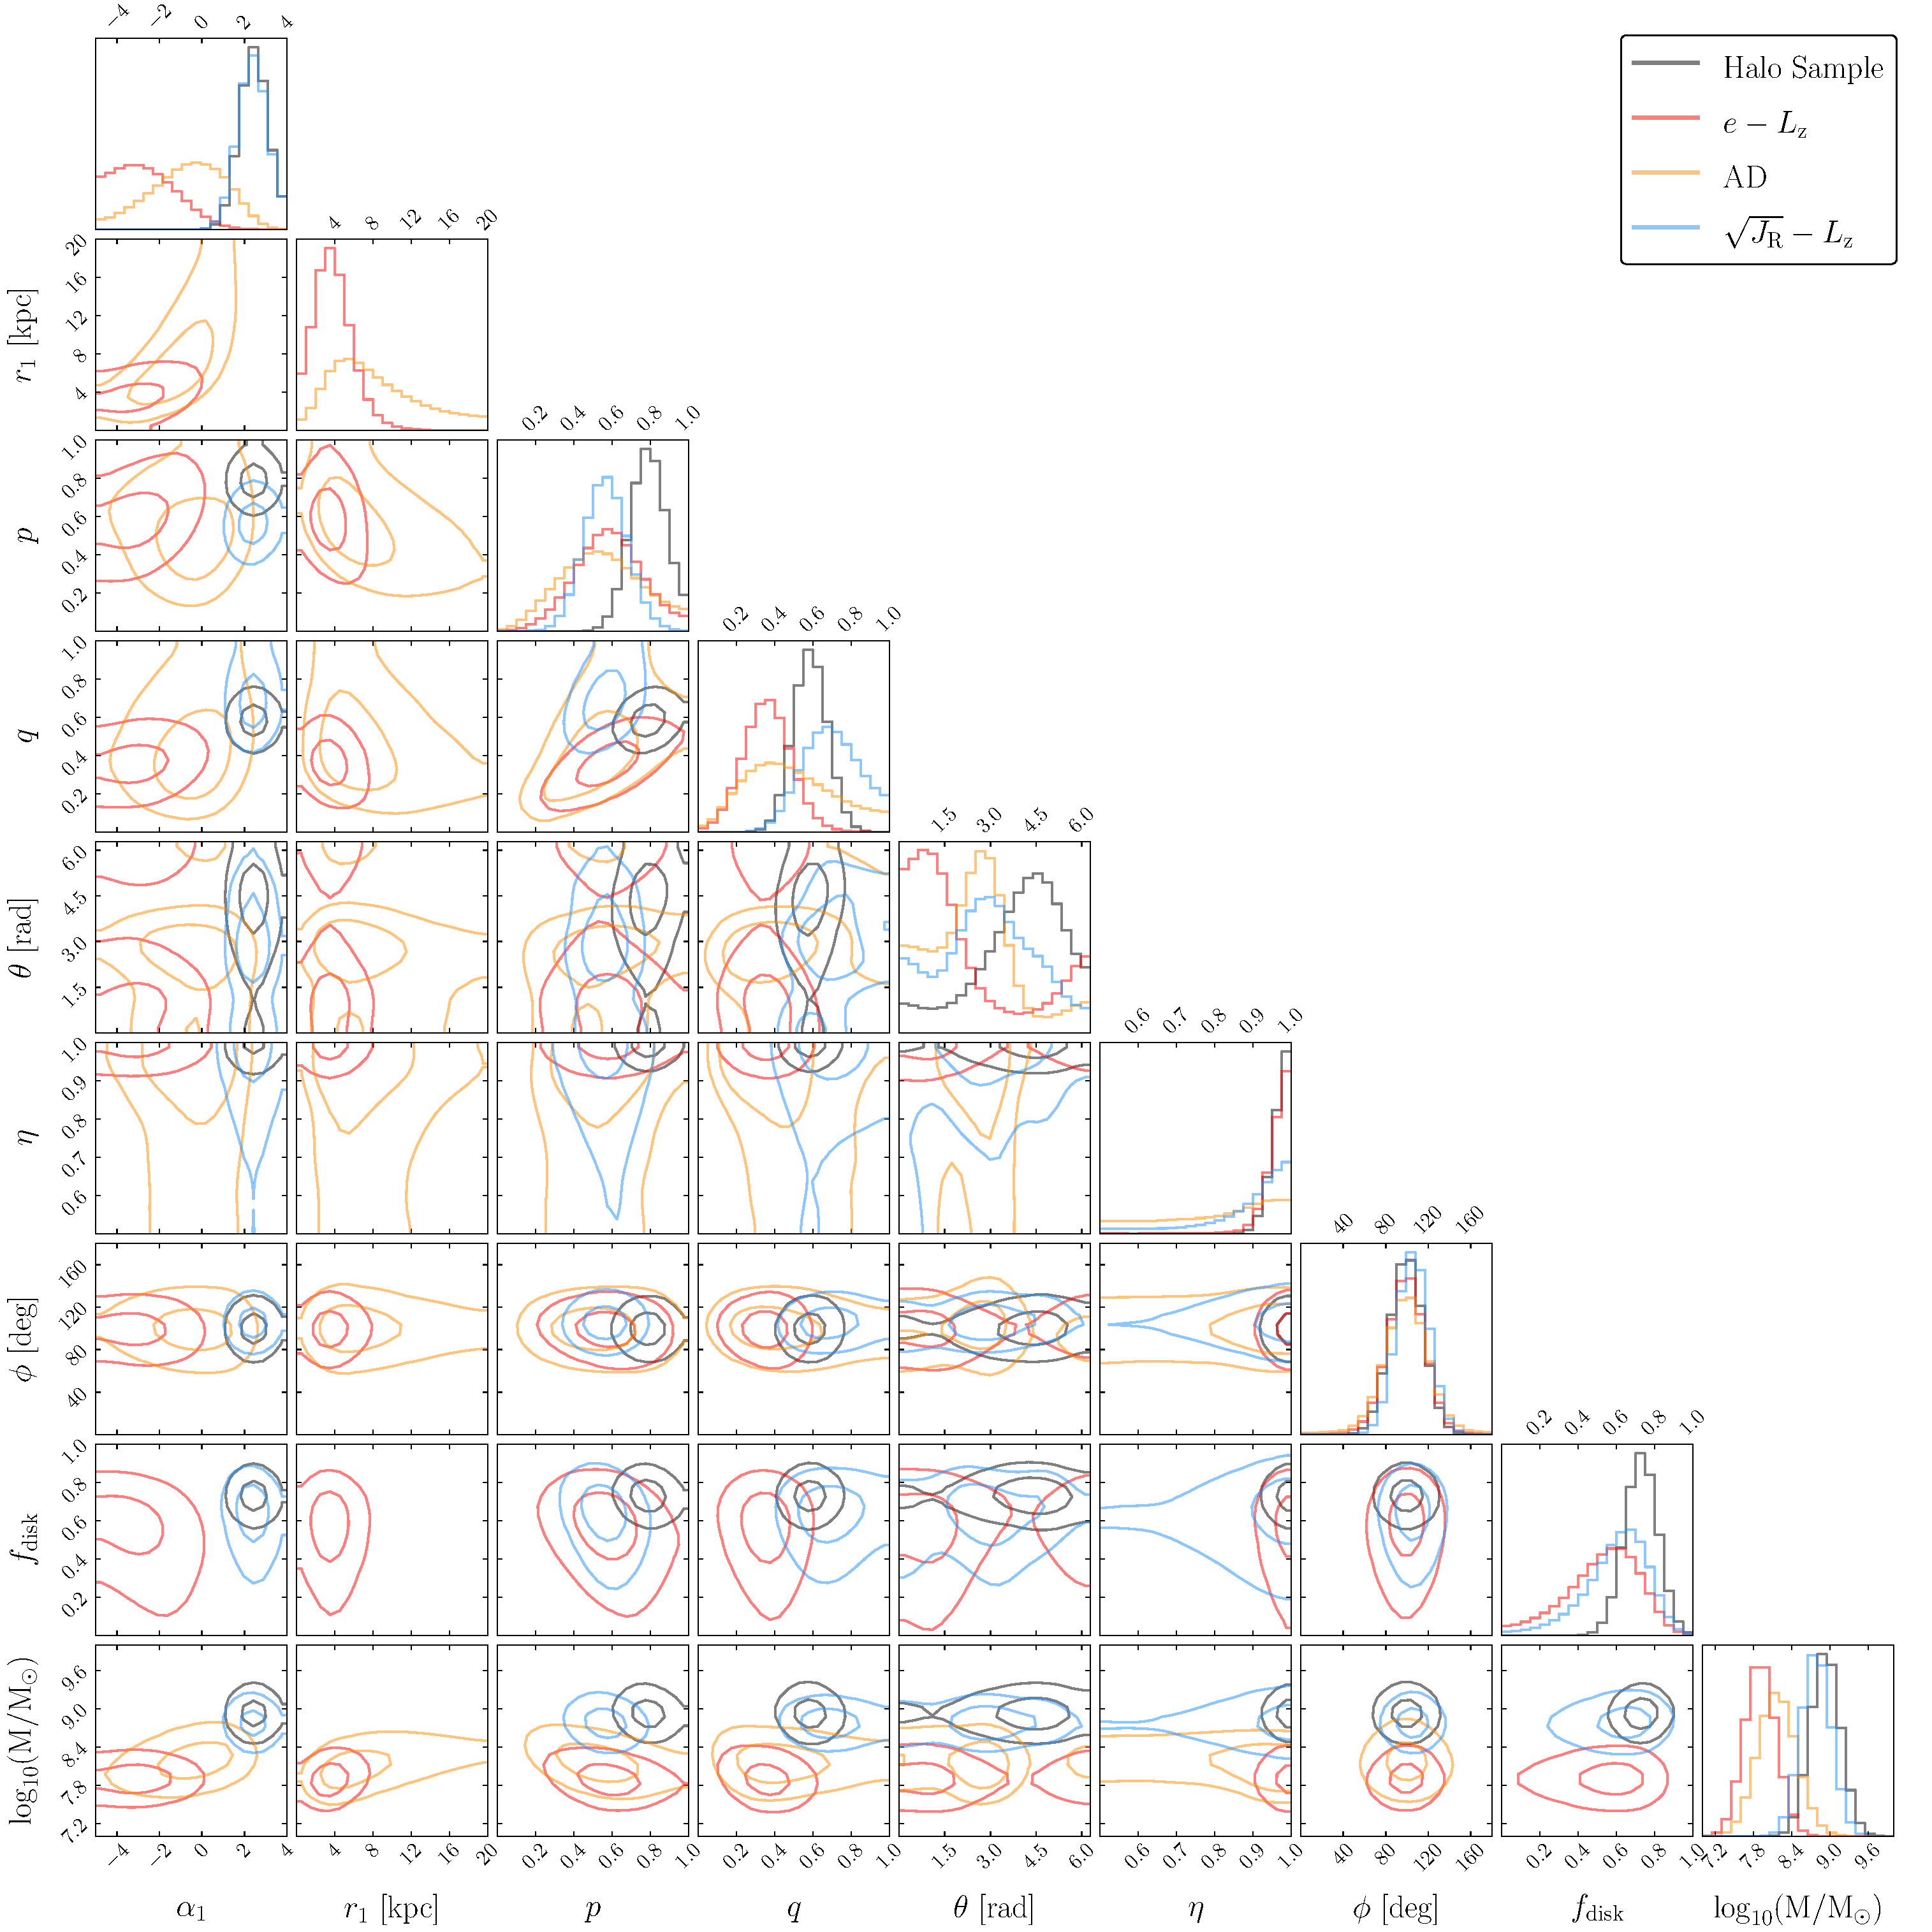
\includegraphics[width=\textwidth]{figure/ch3/posterior.pdf}
    \caption{Corner plot summarizing the results of our best-fitting models for both the halo sample, and GS/E subsamples. Contours are missing when the best-fitting model lacks that specific parameter. The contours are at the 1 and 2 sigma levels.}
    \label{ch3:fig:posterior}
\end{figure}

We do note that even though these goodness-of-fit criteria favour simpler models over more complex models, that the more complex models tend to match the simpler models in the case of each sample. For instance, the SC and BPL models are very similar in regards to shape parameters and derived masses in the case of the \eLz\ and AD samples. While the power law and break radii appear at a glance disimilar, as mentioned above and as we shall show, these profiles are not particularly different. With this in mind, even though the simpler models are favoured from a statistical perspective, we will discuss the results of the BPL and DBPL models, particularly the break radii and different power laws.

\subsection{Fits to the whole halo}

We also performed fits using the same set of density profiles to the whole halo sample, without using any kinematic selection functions but otherwise following the exact procedure laid down in \S~\ref{ch3:sec:method}. We also calculate $\mathrm{max}(\mathcal{L})$, AIC, and BIC with the results. The best-fitting parameters and likelihood-based parameters are shown at the bottom of Tables~\ref{ch3:tab:structural} and \ref{ch3:tab:likelihood} respectively. Best-fitting structural parameters are broadly homogeneous for each of the density profiles. The inner power law index, $\alpha_{1}$, is steeper than for any of the kinematically-selected samples, tending to lie in the range 2.5-2.9. Break radii are somewhat trivial, with the posteriors hugging the upper domain limit of 55~kpc. Shape parameters are not disimilar from the \eLz\ and AD fits, although the halo is much closer to a simple oblate ellipsoid, with $p$ between 0.8 and 0.9 and $q$ taking values between 0.5 and 0.6. Orientation parameters suggest strict alignment with the Galactocentric frame, with $\eta$ very close to 1, which renders $\theta$ uninformative. $\phi$ takes values of about $100\degr$, consistent with the values found for the kinematic samples, suggesting alignment of the major axis of the density ellipsoid with the Galactocentric Y-axis. Finally, $f_\mathrm{disk}$ is higher than for the kinematic subsample fits, with best-fits occupying a narrow range 0.73 -- 0.75, which are equivalent to a numerical contamination fraction of 0.18 -- 0.2.

Masses for the whole halo are much larger than for the GS/E subsamples, lying between $10^{8.8}-10^{8.9}$ ($\sim 6.5-8.5\times10^{8}$)~\Msun\ depending on the density profile. Since the break radii lie at large Galactocentric distances, the fractional difference between SPL and non-SPL models is much less substantial than for the other kinematic subsamples. Taking the same approach to gauging goodness-of-fit as above, we can say that the best-fitting density profile is the SPL+D model.

One interesting trend is that fits to the halo sample are very similar to those for the \JRLz\ sample. Power law indices of the best-fitting models are both about 2.5, and the masses are comparable. The shape parameters are disimilar between the two best-fits, But the orientation parameters are very similar. Both $f_\mathrm{disk}$ and the mass of the \JRLz\ best-fitting profile is more similar to those of the halo best-fitting profile than either the \eLz\ or AD best-fits. All this suggests that perhaps the \JRLz\ selection is not as high in purity as suggested by \cite{lane22}, and the resulting sample may be closer to an intrinsic whole-halo mix of high and low $\beta$ populations, therefore yielding similar fits.

\subsection{Interpretation of results}
\label{ch3:subsec:interpretation-of-results}

Figure~\ref{ch3:fig:pdistmod} shows histograms of the distance modulus distribution for each of the samples considered here: the halo sample as well as the three kinematically-selected GS/E samples. Overlaid on each of the histograms are characteristic distributions of distance modulus from the posteriors of the best-fitting density profiles, calculated by determining the effective volume as a function of distance modulus (marginalized over all fields). These characteristic distributions are derived by taking the median of one hundred different samples from the posterior parameter distribution, selected randomly. While calculating the median of the posterior parameter samples, we also record the 16th and 84th percentile of the distribution at each distance modulus. We then take an average of these percentiles across each of the eight density profiles (SPL, SC, BPL, DBPL with and without disk contamination), which produces the characteristic uncertainty in the model distributions shown in grey at the top of each panel. Each of the density profiles are clearly able to provide reasonable fits to each of the stellar samples, with posteriors lying well within the counting uncertainty ($\sqrt{N}$ error on the counts in each distance modulus bin, shown as grey error bars) of the distance modulus distributions when also factoring in model uncertainty. There are small variations between density profiles for each sample, and particularly for density models with (dashed lines) and without (solid lines) disk contamination. 

\begin{figure}
    \centering
    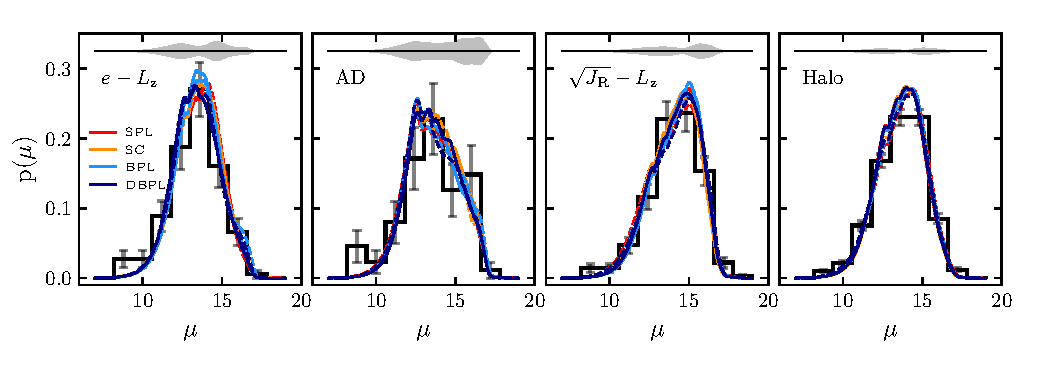
\includegraphics[width=\textwidth]{figure/ch3/pdistmod.pdf}
    \caption{Histograms of distance modulus for each kinematically-selected GS/E sample, labelled by the kinematic selection used, as well as the halo sample. $\sqrt{N}$ counting uncertainty is shown as the grey error bars over each bin in each histogram. Coloured lines show median distance modulus distributions obtained by drawing random samples from the posterior distribution of best-fitting parameters. Dashed lines show density models with disk contamination, and solid lines show density models without disk contamination. The solid grey filled curve at the top of each panel shows the characteristic uncertainty in the distance modulus distribution of density profile fits (see text).}
    \label{ch3:fig:pdistmod}
\end{figure}

Figure~\ref{ch3:fig:pdensity} shows the mass density as a function of triaxial radius $m$ (top panel) and Galactocentric $X$ (bottom panel) for the best-fitting models for each of the samples. The solid lines and the surrounding fill show the median and central 68th percentile confidence interval for the density profile generated using one hundred different sets of parameters, drawn randomly from the posterior distributions. We see emphasized here the similarities between the fits to \eLz\ and AD samples, as well as those between the \JRLz\ and whole-halo samples outlined above. The \eLz\ and AD fits are extremely flat in the inner Galaxy, even rising in the case of the \eLz\ fit, and drop-off precipitously at about $\log_{10}(m/\mathrm{kpc}) \sim 1.2-1.5 = 15-30$~kpc. The \JRLz\ sample best-fit is very similar to the whole-halo fit, a simple power law with nearly identical indices, but offset to lower density.

\begin{figure}
    \centering
    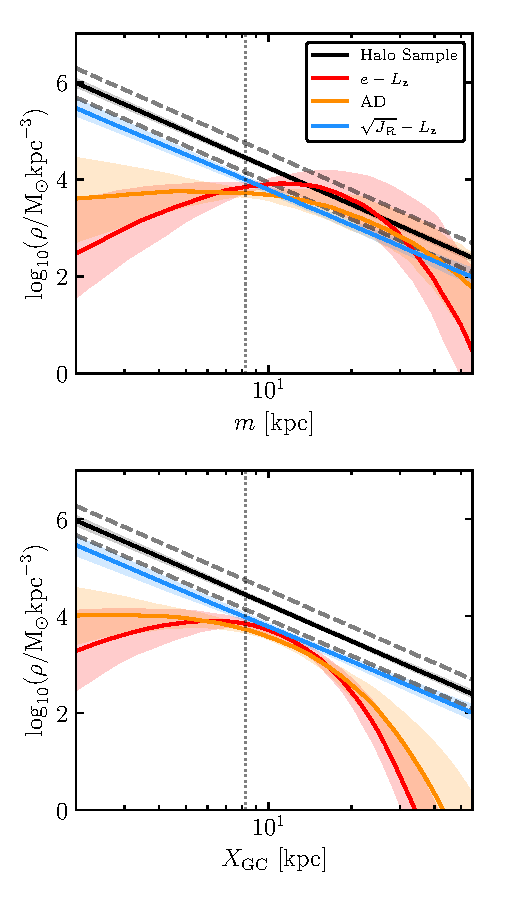
\includegraphics[width=0.5\textwidth]{figure/ch3/pdensity_gcx.pdf}
    \caption{Mass-density posterior for the best-fitting models for the GS/E samples defined by each kinematic selection as well as the whole-halo sample. The top panel shows the density as a function of the triaxial radius $m$ \eqref{ch3:eq:effective-radius}. The bottom panel shows the density along the Galactocentric $X$ axis. In each panel the coloured bands and solid lines show the 68~per~cent interval about the median, respectively, of 100 samples of the density profile parameters drawn from the posterior. The dashed grey lines which parallel the halo profile are fiducials showing a density profile which is twice as heavy (top) and half as heavy (bottom). The dotted line in each panel shows the location of the Sun.}
    \label{ch3:fig:pdensity}
\end{figure}

The dashed grey lines in Figure~\ref{ch3:fig:pdensity} shows density profiles which are half and twice as dense as the median profile for the halo sample. We show these lines because one important consistency check of our results is the observed fact that GS/E constitutes roughly 50~per~cent of stars in the solar vicinity \parencite{belokurov18,lancaster19,fattahi19}. Our GS/E density profile fits do not quite rise to this level, but are not far off, sitting between one quarter to one half of the density of the best-fitting halo model within uncertainties. Interestingly, at slightly larger radii between $\log_{10}(m) \sim 1-1.5 $ or $ m \sim 10-30$~kpc the \eLz\ and AD fits do rise to -- and exceed for a small range of radii -- this level. It is useful here to compare with the density profiles as a function of Galactocentric $X$, which both factor in the effect of $p$ and $q$ and represent the density in a manner more focused on the solar neighbourhood. This panel reveals that indeed the \eLz\ and AD density profiles do peak near the solar vicinity and not beyond, but do not dominate the density at any distance.

Figure~\ref{ch3:fig:pcontour} shows density contours for cross-sectional views of the best-fitting AD profile. We show only one set of density contours, since the approximate shape of the best-fitting profiles is similar among each of the samples (i.e., triaxial, slightly tilted, and with the major axis oriented near the Galactocentric Y-axis). We can now see the density profile described by the best-fitting parameters outlined in in the previous sections. The principal axis of the ellipsoid is rotated towards the Galactocentric Y-axis ($\phi \sim 90^{\circ}$), and is tilted slightly out of the Galactic X-Y plane ($\eta$ near 1). Note that profiles where $\eta$ is equal to 1 will simply have the principal axis in the X-Y plane, but oriented still towards the Y-axis. The inclination of the principal axis with respect to the Galactocentric X-Y plane for the AD best-fitting profile shown here is $-16.4\degr$ (The central 68~percentile interval for this value is $[-35.5\degr,6.6\degr]$).

\begin{figure}
    \centering
    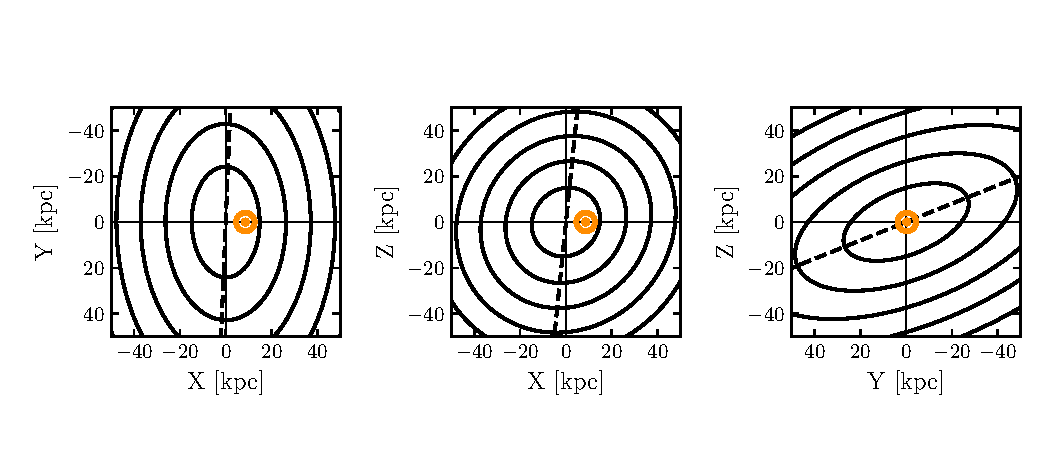
\includegraphics[width=\textwidth]{figure/ch3/contour.pdf}
    \caption{Contours of the best-fitting density profile (SC) for the AD sample. The parameters for the profile are the medians from Table~\ref{ch3:tab:structural}. The density is calculated in each of the X-Y, X-Z, and Y-Z planes, and so is a cross-section. The contours are set at logarithmic number densities (normalized as defined in \S~\ref{ch3:subsec:density-models} such that $\nu_{\star}(\mathrm{R}_{\odot},0,z_{\odot})=1$) of $\log_{10}(\nu_\mathrm{\star}) = [-4.5,-3.5,-2.5,-1.5,-0.5]$. The dashed line shows the principal axis of the 3D ellipsoid, projected on to each plane; it is not guaranteed to align with the cross-sectional density ellipsoids shown in the Figure. The Sun is marked with an orange circle. }
    \label{ch3:fig:pcontour}
\end{figure}

Moving to the mass, in general we find evidence for a light GS/E remnant, roughly $0.8-1.6\times 10^{8}$~\Msun\, in two out of our three kinematic samples under consideration: those created with the \eLz\ and AD selections. The \JRLz\ sample fits suggests the opposite, that GS/E is heavy, roughly $5\times 10^{8}$~\Msun. We posit that this is an issue of contamination, arising from the lower purity of the \JRLz\ selection. Indeed, \cite{lane22} find that the \JRLz\ is the least pure among the kinematic spaces that they studied which we also use here. To further explore this angle, we determine the purity of each of our selections in a manner similar to how we calculated the kinematic effective selection function in \S~\ref{ch3:subsec:kinematic-effective-selection-function}. The purity here is defined as the fraction of samples within each kinematic selection from the high-$\beta$ component with respect to the total number of samples in the selection, from both high- and low-$\beta$ components. We marginalize along each line of sight and over each field, weighted by the effective selection function (which generally describes the number of stars expected at a given location, modulo the density). We find the characteristic purity for the three spaces is as follows: \eLz: 0.84, AD: 0.90, and \JRLz: 0.78. This result is similar to the purity quoted by \cite{lane22} for each space, which was derived using similar models, albeit in a different manner.

A lower purity would impact the results to the fits in two ways. First, more stars would be counted in the fitting sample, which would drive up the normalization factor for the density profiles in equation~\eqref{ch3:eq:density-normalization}, which in turns drives up the calculated masses (see discussion of this effect in \S~\ref{ch3:subsec:method-validation} in the context of our mock data). A second, more subtle, effect is that we would expect the fit to tend more closely to the fit to the whole halo sample. The best-fitting density profile for the halo sample is steep in the inner part of the Galaxy, and lacks a cutoff at 20 to 40~kpc such as the \eLz\ and AD best-fitting density profiles have. Both of these effects contribute to a heavier overall mass, and if the \JRLz\ profile were to trend towards that sort of fit due to lower purity in the underlying sample then we would expect the mass to come out large for that reason as well. Although, it may be argued that the difference in purity (of order 6 to 12~per~cent) between the \JRLz\ and \eLz/AD spaces could not possibly account for this difference. We also acknowledge that the \JRLz\ space is `absolute' in the sense that the dependant variable is the radial action. This is contrasted to the AD and \eLz\ spaces which are much more regular, the AD space being explicitely normalized by the total action, while the \eLz\ space being normalized in the sense that eccentricity may only vary between 0 and 1, and our selection includes eccentricity of 1, which orbits approach as they become increasingly radial. The kinematic effective selection functions are derived assuming a potential, specifically \texttt{MWPotential2014} of \textcite{bovy15}, but it is applied to real data. Now the actions and conserved quantities of the real data are also derived assuming the \texttt{MWPotential2014}, however their underlying kinematics are dictated by the true potential of the Galaxy, whereas the kinematics of the DF samples used to compute the kinematic effective selection function are dictated by \texttt{MWPotential2014}. This mismatch could cause problems for spaces such as \JRLz, which will be much more sensitive to the underlying potential than the AD or \eLz\ spaces.

Interestingly, the works of \textcite{feuillet20} and \parencite{carrillo23} suggest the opposite of the conclusion at which we have arrived here, and they posit that \JRLz\ is the superior space for selecting GS/E debris. \textcite{feuillet20} conclude this by studying the metallicity distribution functions of kinematically selected halo stars, although they do not consider eccentricity or a space similar to the action diamond, finding that \JRLz\ is better than energy versus $L_\mathrm{z}$, the Toomre diagram, and radial versus tangential velocities \parencite[this is actually consistent with the conclusions of ][]{lane22}. So while they determine that \JRLz\ is better than energies and velocities we should not take that to mean that eccentricities and the action diamond may not be better than \JRLz. \textcite{carrillo23} come to their conclusions while studying simulated GS/E remnants in a cosmological context. They consider all of the spaces studied by \cite{lane22} but use different specific kinematic selections in some instances. For example they consider eccentricities greater than 0.7 (our eccentricity selection which is very close to 1), and a slightly larger selection in the action diamond. Their findings regarding eccentricity are broadly consistent with \cite{lane22}, who also find that $e > 0.7$ yields poor purity (again, note the eccentricity selection used in this work is much more restrictive). With respect to the action diamond, their results are tougher to reconcile with those of \cite{lane22} since the selections are similar, although their selection is again broader. In general, the work of \textcite{carrillo23} benefits from knowledge of the ground truth and the realistic dynamics innate to simulations, however they lack the necessary abundance information in their simulations with which to make cuts which are typical in observations. So while perhaps their work does not discount our conclusions about the purity of kinematic spaces it certainly highlights the need to take care when kinematically selecting GS/E debris. Finally, the work of \textcite{donlon23} suggests that \JRLz\ may be contaminated at high $\sqrt{J_\mathrm{R}}$ at the level of $\sim 1/3$ or greater by non-GS/E accretion remnants, which is in rough agreement with the findings of \cite{lane22}.

\subsection{Altering the kinematic effective selection}
\label{ch3:subsec:altering-kinematic-effective-selection-function}

When constructing the kinematic effective selection function, we noted the inconsistency between the fact that we had to assert a density profile for the stellar halo when defining the DFs, yet we are employing the DFs to determine the density profile of the stellar halo. To investigate the impact of this assumption, we compute new high and low-$\beta$ DFs based on the density profiles that we have determined for the GS/E and whole-halo samples. For the low-$\beta$ component we construct a density profile inspired by the best-fitting SPL model to the whole-halo sample. We use a single power law density profile with index $\alpha=2.5$, normalized such that it has a mass of $6\times10^{8}$~\Msun\ between $2-70$~kpc (i.e. roughly the mass of our whole-halo fit less our mass derived for the GS/E remnant). For the high-$\beta$ component we take our cue for the density profile from the BPL fits, which for the AD and \eLz\ samples have approximate inner and outer power laws of 0.8-1.2 and 3.8-5.2, and break radii between 17-27~kpc. We therefore conveniently approximate the high-$\beta$ component using a Hernquist density profile \parencite{hernquist90}, which has an inner power-law index of 1 and an outer index of 4, with scale radius 20~kpc and a mass between 2-70~kpc of $1.5\times10^{8}$~\Msun. We choose to model the high-$\beta$ density profile in this way for ease of computation, and the BPL models which inspire it provide fits to the data with equivalent likelihood compared with the SC model which is our claimed preference. We keep the values of $\beta$ fixed at 0.3 and 0.8.

Samples are drawn and kinematic quantities are computed as outlined in \S~\ref{ch3:subsec:kinematic-effective-selection-function}. Now, however, we compute purity by counting the number of high-$\beta$ samples in each selection with respect to the total number of samples, but we weight the contributions from the low and high-$\beta$ components by the local density of the respective density profile (note the completeness of the high-$\beta$ component is independent of the local densities of the two components). We replicate Figures~\ref{ch3:fig:ksf_dmod_fields} and \ref{ch3:fig:ksf_lb_dmod_marginalized}, which show the kinematic effective selection functions, as Figures~\ref{ch3:fig:ksf2_dmod_fields} and \ref{ch3:fig:ksf2_lb_dmod_marginalized}, which are shown in Appendix~\ref{ch3:ap:modified-ksf}. Examining the new kinematic effective selection function (which we denote at $\mathfrak{S}_{2}^{\prime}$ in these figures) reveals remarkable consistency between them and the original kinematic effective selection functions shown in Figures~\ref{ch3:fig:ksf_dmod_fields} and \ref{ch3:fig:ksf_lb_dmod_marginalized}. On Figure~\ref{ch3:fig:ksf2_dmod_fields} we overlay the median trends, calculated across all fields at each distance modulus, of each of the kinematic effective selection functions to summarize the differences. The overall typical value of $\mathfrak{S}_{2}$ decreases slightly for each selection, from $\sim 0.5$ to $\sim 0.45$ for the \eLz\ space for example, but the overall form remains very similar. This implies that we could expect very similar fits to the data using these new kinematic effective selection functions, except that the derived mass should increase by a small amount, since the typical value of $\mathfrak{S}_{2}$ is somewhat smaller. We compute the ratio between these two median trends, and calculate an average over the range of distance modulus weighting by the distribution of distance moduli in the sample (top panel in Figure~\ref{ch3:fig:ksf2_dmod_fields} which is the same as the top panel of Figure~\ref{ch3:fig:ksf_dmod_fields}). We find that the resulting typical fractional change in the kinematic effective selection function is -0.09 (\eLz), -0.07 (AD), and -0.13 (\JRLz). We would therefore expect the masses to increase by a small amount, roughly 10~per~cent, but overall this effect is negligible. In general, these results suggest that the DF-based corrections we derive and apply in our modelling framework are resilient to modest changes, and therefore that as long as the assumptions underlying the models used to generate the corrections are realistic that their specific form is generally unimportant.

The most interesting aspect of this analysis is actually in examining purity. Above we noted that the purity is lower for the \JRLz\ selection than the \eLz\ or AD selections, but not by a significant amount (0.78 versus 0.84 and 0.9 respectively). We recalculate the typical purity using the new DFs here, again by summing the purity over all fields and distances weighted by the value of the effective selection function. We find that the new purity values are 0.78 for the AD selection, 0.65 for the \eLz\ selection, and 0.52 for the \JRLz\ selection, so all values have been lowered. Note that the overall lowering of the purities here will be largely driven by the fact that the low-$\beta$ density profile is quadruple the density at the solar position compared with the high-$\beta$ component. This should not be taken as indication that these selections are now inferior, and they are likely still optimal (i.e. were one to repeat the analysis of \cite{lane22}). The differences in purity among the kinematic spaces are even more stark now than in the case of the original DF models, and suggest that \JRLz\ is truly an inferior kinematic space for which to select GS/E samples. Fractionally, the \JRLz\ space experiences the largest reduction in purity, decreasing 33~per~cent. The fractional decrease for the \eLz\ and AD spaces are smaller in magnitude, 22 and 14~per~cent respectively. So not only does the AD space maintain the highest purity, but its purity is changed by the smallest amount when pivoting from the original DF models to those based on our results. These findings suggest that the AD space, in particular, should be preferred given its high purity and resilience of its purity to changes in DF models.

\subsection{Our preferred results for the density profile of GS/E}

We close out this section by summarizing our main findings for the density profile and mass of GS/E in light of our primary results and secondary analyses. We have already noted that there appears to be broad consensus between the fits to the \eLz\ and AD samples, a consensus which differs significantly from the results of the \JRLz\ sample. We also noted that the results for the \JRLz\ sample are similar in many ways to the results for the fits to the whole halo. When factoring in the assessment of purity, for both the original kinematic effective selection functions and the second set of kinematic effective selection functions derived based on our initial results, we arrive at a neat conclusion. The \eLz\ and AD results more faithfully trace the underlying reality of the GS/E remnant, while the \JRLz\ results are biased by excessive contamination from the low-$\beta$ halo such that the density profile parameters are similar to those for the whole halo and the mass is overestimated. For this reason we defer to the former results, and specifically those for the AD sample since it has the highest purity, when crafting our conclusions regarding the density profile and mass of GS/E.

With this in mind we can say that the best-fitting density profile for the GS/E remnant is the SC model, a single power law with exponential truncation, with $\alpha_{1} = -0.57^{+1.58}_{1.95}$ and $r_{1} = 8.57^{+12.58}_{-4.36}$~kpc. This type of density profile, which gently rises in the inner Galaxy and drops rapidly at modest Galactocentric radii, is non-traditional. For this reason we also report the power law indices and break radius of our BPL fit (no disk contamination) which has inner power law $\alpha_{1} = 1.05^{+0.86}_{-0.72}$, outer power law $\alpha_{2} = 3.79^{+2.44}_{-0.98}$, and break radius $r_{1} = 23.59^{+15.55}_{-9.30}$~kpc. These two profiles are, in practice, very similar over the range of radii probed and are equivalent in terms of maximum likelihood, yet the SC model is favoured by BIC/AIC since it has one fewer parameter. We find that GS/E is moderately triaxial, with the ratios of the Y-X and Z-X axes in the rotated (not Galactocentric) frame being respectively $p = 0.54^{+0.22}_{-0.2}$ and $q = 0.46^{+0.27}_{-0.2}$. The principal axis is rotated towards the direction of Galactic rotation with $\phi = 99.5^{+13.9}_{-14.9}$ degrees, and is tilted slightly out of the Galactic plane with $\eta=0.84^{+0.12}_{-0.22}$ and $\theta = 147.0^{+43.5}_{-95.3}$ degrees, which equates to an inclination of the principal axis of $-16.4^{+23.0}_{-19.1}$ degrees. Finally, the mass is $1.45^{+0.92}_{-0.51}\times10^{8}$~\Msun. 

We also calculate a few supplementary parameters that derive from our best-fitting density profile and associated mass. First, we consider the triaxiality parameter, $T$, commonly given as

\begin{equation}
    T = \frac{1-(b/a)^{2}}{1-(c/a)^{2}}
\end{equation}

\noindent where $b = \mathrm{max}([p,q])$ and $c = \mathrm{min}([p,q])$ in the context of our model parameters, and $a=1$. We calculate this parameter for each of the samples in the posterior for the SC fit to the AD sample, arriving at a value of $T=0.79^{+0.13}_{-0.35}$. This indicates that the GS/E density profile is preferrably prolate, but only to a modest degree. Second, we take our stellar mass and determine the corresponding dark matter halo mass using a stellar mass--halo mass ($M_{200}$) relation. According to the relation derived by \textcite{behroozi13} (and validated by \textcite{read17} for stellar masses $\sim10^{8}$~\Msun) a stellar mass of $1.5\times10^{8}$~\Msun\ implies a halo mass of about $5\times10^{10}$~\Msun\ at redshift $z=0$, with halo masses larger by a few tenths of a decade expected for the same stellar mass at redshift $z=2$ (the approximate GS/E merger epoch). The Milky Way-oriented stellar mass--halo mass relation of \textcite{nadler20} predicts a comparable halo mass of $6\times10^{10}$~\Msun. Given that the Milky Way at the time of the merger had a halo mass that is approximately half of that today \parencite[so $\approx 5\times 10^{11}$~\Msun; e.g.][]{mackereth18a}, this means that the GS/E merger was approximately 1:8 to 1:10, constituting a minor merger.

\section{Discussion}
\label{ch3:sec:discussion}

\subsection{The distribution function models and the kinematic effective selection function}
\label{ch3:subsec:df-models-ksf-discussion}

Our results presented here are perched upon the DF-based models introduced by \cite{lane22}. While we have gone to great lengths in this paper to demonstrate that the corrections we derive for kinematic selections allow recovery of the properties of the underlying population, we must address the limits of these types of models. First, the functional form of our DFs is a simple, but flexible, \textit{ansatz} \eqref{ch3:eq:anisotropic-df} which is designed to incorporate many of the basic features we expect from stellar halo populations: simple radial dependency and a variable anisotropy which is assumed to be radially constant. It lacks, however, many of the ingredients that we know stellar halo populations to possess. For example, we know that GS/E is likely to have modest net rotation \parencite{helmi18,lancaster19,iorio21}, and to have asymmetric or complicated phase-space features when comparing the debris at high and low $L_\mathrm{z}$ \parencite{helmi18,naidu20}, or at large Galactocentric radii \parencite{chandra23}. Additionally, as we have shown here and as has been shown in nearly every other work that has measured the density profile of GS/E, the remnant is triaxial \parencite{iorio19,han22}. None of these features are included in our DF models (but of course our density models are triaxial), which may result in discrepancies between our corrected results and the true GS/E population which are challenging to predict. Finally, the mathematical form of the DF implies divergence when $\beta > 0$ as $L \rightarrow 0$, which may compromise its suitability for modelling purposes \parencite[as discussed by ][]{binney14d}. These effects may be particularly exacerbated when modelling the highly anisotropic GS/E remnant.

Despite these admitted deficits, our models do an excellent job of reproducing the basic assumptions and features of GS/E, namely that it is a stellar population with extreme radial anisotropy and near-zero $L_\mathrm{z}$ \parencite[see figure 4 in][for example]{lane22}. It is likely that our models are closer to a true description of the phase-space density of GS/E than not, and therefore that our results should be taken at face value. \cite{lane22} tested their models against changes in underlying potential, and they also tested the resiliency of their selections to changes in radius, finding that neither change produced a noticeable effect on the interpretation of their results. Those findings may be carried over to our work to suggest that our results would be resilient to changes in underlying potential as well, while variations the quality of the selection with radial position are explicitely handled by our spatially-dependent kinematic effective selection function. Additionally, we explored variation in the kinematic effective selection function and found that at least one of our kinematic selections, AD, is resilient to iterative improvements in the selection function based on our initial results. These tests all suggest that our preferred findings of a light, triaxial GS/E are accurate and would not change substantially given more sophisticated corrections based on more realistic kinematic models.

Despite our confidence in these results, we do plan follow-up work which will both help to reinforce our findings, but also to expand these sorts of techniques for use with other remnants, which tend to have more complicated kinematic properties, requiring more complicated kinematic selections and corrections during the modelling procedure. A tangential, yet perhaps more realistic, approach would be to model the stellar halo as a mixture of self-consistent DFs \parencite[see, e.g.][for similar studies using Gaussian mixtures]{lancaster19,iorio21}, however the large number of parameters and the intractability of computing such DFs on the fly mean that it would be somewhat challenging. On a similar note, exploring the use of more realistic DFs should be of top priority. For example action-based DFs \parencite{binney14d,posti15,williams15} including flattening and rotation \parencite{binney14d}. The construction of self-consistent triaxial DFs is an area of ongoing effort \parencite{sanders15a,binney18}, yet these would obviously prove ideal given the observed geometry of the GS/E remnant.

Another fruitful avenue for future work would to test these sorts of modelling techniques on merger remnants in simulated Milky Way analogs sourced from cosmological simulations. The EAGLE \parencite{schaye15}, AURIGA \parencite{grand17}, and FIRE \parencite{wetzel16} sets of simulations, among others, all have rich veins of recent work on GS/E-like remnants \parencite[e.g.][]{fattahi19,mackereth19a,horta23b,orkney23}. In particular, examining the phase space distributions of debris in detail would be useful. There have been recent works that have looked at the phase space distribution of simulated debris \parencite[e.g.][]{amorisco17,jean-baptiste17,naidu21,amarante22,orkney23,carrillo23}, and we advocate a more in-depth look specifically at how well various families of DFs can be fit to merger debris. This type of study could place necessary constraints or priors on the vast volume of parameter space which would undoubtedly accompany a multi-DF assessment of the Milky Way stellar halo.

\subsection{The measurement of the mass of the GS/E remnant}

The core measurement made in this paper is the stellar mass of GS/E, which we estimate to be about $1.5\times10^{8}$~\Msun\ in our best-fitting models. We will discuss our results in the context of the literature in the next section, but so as to not bury the lead: our derived mass for GS/E is much lower than other findings. It therefore behooves us to assess our measurement of the mass of GS/E and investigate possible sources of systematic error.

First, we examine the impact of a few of our sample-selection and model-fitting decisions on our final results. We repeat our fits without the $\log g$ uncertainty and relative distance uncertainty cuts presented in \S~\ref{ch3:subsec:observations}. The Halo sample and the three GS/E samples increase in size by between 2--8~per~cent when these cuts are removed, but the changes to the results -- the values of the best-fitting parameters, the derived masses, and the overall narrative presented in \S~\ref{ch3:sec:results} -- are negligible. According to the BIC/AIC the best-fitting density profiles are the same for the Halo sample and each of the three GS/E samples, and the masses change by only a few per~cent (the fit to the AD sample increases by 0.01 dex), far smaller than the statistical uncertainty on each measurement. We also check the assumptions which go into the construction of the effective selection function and the density profile normalization factors, namely the choice of [Fe/H] and age ranges. While \textcite{montalban21} show that typical GS/E stars ages are about 10~Gyr old, the distribution extends down to $\sim 7$~Gyr old. Additionally, with regards to our choice of [Fe/H] range, whereas we elected to use a minimum [Fe/H] of -3 for the halo sample, the data only barely extend lower than [Fe/H] of -2. We replicate our fits but using a new isochrone grid which extends from 7-14~Gyr old (therefore rebuilding our effective selection function) and using a minimum [Fe/H] of -2 for the halo population (same as for the GS/E samples), but holding all other aspects of our analysis constant. We again find that this has a negligible impact on our results or overall narrative. Masses decrease by between 0.02 and 0.07 dex (the largest decrease is for the AD GS/E sample), best-fitting density profile parameters change little, and the AIC/BIC prefer the same density profiles. We therefore assign a systematic uncertainty which lowers the mass of GS/E by 0.07 dex (15~per~cent), or about $0.22\times10^{8}$~\Msun, due to choices in parameters for sample selection and effective selection function grid construction.

Second, as discussed when validating our method in \S~\ref{ch3:subsec:method-validation}, we expect the mass of our fits to be slightly overestimated due to contamination from the low-$\beta$ component. Now in the case of the mock data, both the low and high-$\beta$ components were drawn from the same density profile, and therefore one would only expect bias due to the excess in number counts (modulo some higher order effects from the spatial dependence of the selection). Secondarily, and as discussed above in the context of the disparity between \eLz\ and AD fits versus \JRLz\ and whole-halo fits, when the underlying density profiles differ then contamination from the low-$\beta$ component can lead to a best-fitting density profile which more closely resembles that of the low-$\beta$ component than the target density profile of the high-$\beta$ component. Given that we assume the low-$\beta$ component has a `more massive' density profile (i.e. the whole halo has a steeper power law in the inner Galaxy and a less marked break at intermediate Galactocentric radii) then we might also expect that contamination leads to an overestimation of the mass.

The first of these effects is simple to gauge: we expect to overestimate the mass by a factor equal to the inverse of the purity of the selection (this is neatly observed when determining the mass of our mocks). In the case of the AD selection the purity is estimated to be 0.9 for our initial kinematic effective selection function, and drops to 0.78 for our more realistic kinematic effective selection function created in \S~\ref{ch3:subsec:altering-kinematic-effective-selection-function}. The purity found by \cite{lane22} for the AD selection was 0.86. The second effect, the biasing of the shape of the density profile itself is challenging to gauge. We have posited above that contamination from the low-$\beta$ halo causes the increased mass found with the \JRLz\ fit, however this is higher than that for the AD fits by a factor of 3-4. Without any good way to gauge the impact of the contamination on the shape of the GS/E halo density profile we therefore fall back on the simple, conservative estimate being of order the inverse purity. We therefore adopt as our first systematic uncertainty one which lowers the mass to 0.78 (the lowest purity estimate for the AD selection) times the best-fitting mass, which is about $0.3\times10^{8}$~\Msun. We do note though that we have attempted to mitigate this source of systematic uncertainty by cutting stars with high [Al/Fe] from our kinematically-selected GS/E samples (see Figure~\ref{ch3:fig:halo_abundances}), since these stars are more likely to be part of the \textit{in-situ}, low-$\beta$ stellar halo.

Building on this, while we believe the trimming of stars with high [Al/Fe] is a well-motivated way to remove low-$\beta$ and thick disk contaminants from our kinematic selections, it is possible that these are genuine GS/E stars which should be included in our calculations. For the AD selection there are 4 stars which are removed on this basis, compared with 73 stars in the sample (there are similar fractions removed for the \eLz\ and \JRLz\ spaces, of order 5-8~per~cent). Assuming that inclusion of these stars would not change the density profile, only increase the normalization factor, this would result in an increase in the mass by $0.08\times10^{8}$~\Msun.

Finally, we consider that in \S~\ref{ch3:subsec:altering-kinematic-effective-selection-function} we investigated iterative improvements to the kinematic effective selection function, finding that more realistic kinematic effective selection functions constructed based on our fits generally have smaller values for a fixed kinematic selection. For example, referring to Figure~\ref{ch3:fig:ksf2_lb_dmod_marginalized} we see a typical value of 0.5 for the value of $\mathfrak{S}_{2}$ for the AD selection, while a typical value for the more realistic $\mathfrak{S}_{2}^{\prime}$ is more like 0.45. In \S~\ref{ch3:subsec:altering-kinematic-effective-selection-function} we specifically calculated a fractional decrease for the AD space of -0.07. Again, since this is for a fixed kinematic selection, and therefore a constant number of stars in the sample, we expect this decrease in the value of the kinematic effective selection function to manifest as an increase in the derived mass by an approximate factor $0.07$, or about $0.1\times10^{8}$~\Msun.

Before summarizing our systematics we discuss three related points. First, we must contend with the fact that we find a much lower fractional density for the high-$\beta$ GS/E component at the position of the Sun compared with other studies, which tend to attribute about 50~per~cent of the density near the Sun to GS/E \parencite{belokurov18,lancaster19,iorio21}. We find that the density at the position of the Sun for the AD sample is $\nu_{0} = A\chi = 5.2^{+0.7}_{-0.6}\times 10^{3}$~\Msun~kpc$^{-3}$, compared with a density of $2.7^{+0.2}_{-0.2}\times 10^{4}$~\Msun~kpc$^{-3}$ for the halo sample. This is a difference by about a factor of 5, about 2.5 less than we would expect for an even mixture of high- and low-$\beta$ stars at the solar position. Since in our analysis mass scales directly with the density at the solar position, if we demand that the density of the GS/E component rises to the level of 50~per~cent of the whole-halo sample, then we would find the mass increases to about $3.8\times10^{8}$~\Msun. Now, we do not consider this to be a genuine source of systematic uncertainty, unlike those noted above, since we have no reason based on a sober assessment of our analysis to think that we have substantially underestimated the density at the solar position. For this reason we simply note that this is what our mass would become in light of these constraints from prior studies.

A second point is that we elected to model the high-$\beta$ portion of the stellar halo using an anisotropy of $\beta=0.8$ to avoid minor numerical instabilities noted by \cite{lane22} when using DFs with $\beta=0.9$. This is slightly lower than the value of $\beta \approx 0.9$ which is preferred by recent literature \parencite{belokurov18,fattahi19,lancaster19,iorio21}. Our choice of $\beta=0.8$ actually implies that our derived mass is an upper limit, assuming that the geometry and form of the best-fitting GS/E density profile would be similar if we fit with a kinematic effective selection function derived using $\beta=0.9$. This is because the kinematic effective selection function should typically approach 1 as $\beta$ increases, which in turn decreases the derived mass. Intuitively, the selections from \cite{lane22} contain within them a larger fraction of a $\beta=0.9$ population than a $\beta=0.8$ population since they probe regions of kinematic space where extremely radial orbits lie, and therefore the required correction for stars missed by the restrictive kinematic cuts is smaller and the inferred mass is smaller. To check this explicitly, we compute a kinematic effective selection function assuming the same parameters as presented in \S~\ref{ch3:subsec:kinematic-effective-selection-function} except that we increase the high-$\beta$ anisotropy to 0.9. We find that the form of the correction is very similar to the $\beta=0.8$ correction both as a function of distance along each line of sight, as well as on-sky position, except that values are as expected systematically higher. For the AD space, we find typical values increase from $\sim 0.4$ to $\sim 0.6$, and similarly for the \eLz\ space we find typical values increase from $\sim 0.5$ to $\sim 0.7$. Assuming that were we to fit our samples with these kinematic effective selection functions that resulting density profiles would be similar to our current findings, we can say that the derived mass would be about 60-70~per~cent our current derived mass, or about $1\times10^{8}$~\Msun.

A third and final auxilliary point is to mention that while we are confident in our thick disk outlier model, it is possible that it does not fully capture all possible contaminants. It is well known that the thick disk has a range of geometries depending on the age and abundance of the specific sub-population \parencite{bovy12d,mackereth19b}, and the oldest, hottest, thickest parts may not be well-described by our simple single-exponential model. This is less likely to impact the measurement of the mass of GS/E, since these contaminants likely have higher [$\alpha$/Fe] and [Al/Fe] such that they are excluded from our chemical cuts on the GS/E subsamples. The whole-halo sample, on the other hand, may be plagued by such contaminants since it includes higher [Al/Fe] stars. It may be the case then, that our measurements of the total mass of the stellar halo are impacted, and by extension our estimates of the mass ratio of the GS/E merger. However since our stellar halo mass measurements are less than $10^{9}$~\Msun\ and therefore on the low end of modern estimates \parencite[e.g.][]{deason19,mackereth20} it is likely that the degree of contamination is minimal.

Now by combining the sources of systematic uncertainty together, and adding uncertainties in quadrature, we arrive at an estimate for the mass including systematics of $1.45\ ^{+0.92}_{-0.51} \mathrm{(stat.)}\ ^{+0.13}_{-0.37} \mathrm{(sys.)}\ \times10^{8}$~\Msun. And to be clear we have not included the overestimations due to the discrepency between our measured fractional solar densities for GS/E and the literature estimates, or the modification of the mass due to a change in $\beta$ in this quoted value.

\subsection{Comparison of our findings with other work}
\label{ch3:subsec:comparison-with-other-work}

It is challenging to compare our results with those of other studies due to the unique nature by which we select our sample. Although the spirit of our kinematic and chemical selections is not that different from similar studies \parencite[e.g.][]{mackereth20,han22}, our kinematic selections are far more restrictive and we correct for missing stars using a novel kinematic effective selection function. None the less, we attempt here to provide a context for the density profile parameters and mass of GS/E reported here.

\subsubsection{The mass of GS/E}

When it was first studied after its discovery, the stellar mass of the GS/E progenitor was thought to be quite high. \textcite{helmi18} posited the stellar mass was $6\times10^{8}$~\Msun\ based on chemical abundance trends, and \textcite{belokurov18} suggested that the virial mass of the progenitor was $> 10^{10}$~\Msun. Early simulation-based studies suggested that the stellar mass of the progenitor could by in the range $10^{8.5}-10^{10}$~\Msun\ \parencite{fattahi19,mackereth19a}.  In particular, \textcite{fattahi19} find that within 20~kpc the mass of the progenitor could be between about $2\times10^{8} - 2\times10^{9}$~\Msun. \textcite{das20} estimate a total virial mass of about $10^{11}$~\Msun\ based on the dispersion of the remnant in action space, which equates to a stellar mass of about $10^{9.5}$~\Msun\ using canonical abundance matching relations. GS/E was also studied using chemistry, with \textcite{vincenzo19} estimating a mass of $5\times10^{9}$\Msun\ and \textcite{feuillet20} estimating a mass of $7\times10^{8} - 7\times10^{9}$~\Msun. \textcite{naidu20} and \textcite{naidu21} use H3 data -- and N-body simulations in the latter study -- to infer a mass in the range of $4-7\times10^{8}$~\Msun. The work of \textcite{naidu21}, where the mass was found to be $5\times10^{8}$~\Msun, in particular is consistent with a number of auxilliary constraints on GS/E, such as the modestly retrograde tendancy for the debris \parencite{belokurov18,helmi18}, the existence of a retrograde tail of debris at large $L_\mathrm{z}$ \parencite{helmi18,naidu20}, as well as the concurrence and alignment with the major axes of the density ellipsoid of the debris with the Hercules-Aquila Cloud and the Virgo Overdensity \parencite[first noted by][]{simion19}. More recently, \textcite{rey23} use the VINTERGATEN suite of cosmological zoom simulations to study GS/E-like mergers of varying mass ratios using the `genetic modification' technique. Their results favour a similar mass ratio for the GS/E merger as our finding, but most interestingly they demonstrate that a wide range of merger mass ratios ($\sim 1:24 - 1:2$) can lead to very similar halo chemodynamics at $z=0$. This may help to explain why our results are at odds with many of the abundance-based measurements which predict a higher mass for GS/E.

The work of \cite{mackereth20} is the most closely analogous to ours, since they use a very similar technique, similar density profiles, and similar sample (they use APOGEE DR14). They find the mass of GS/E to be approximately $3\times10^{8}$~\Msun, although they base this estimate purely on a chemical selection of GS/E inspired by \textcite{mackereth19a}. Another recent work which is very similar to ours is that of \textcite{han22}, who fit triaxial broken power law density profiles to H3 data, finding a mass of $5.8-7.6\times10^{8}$~\Msun, with the lower mass end of that range corresponding to more restrictive eccentricity cuts on the GS/E sample. Compared to all of these works, we find a much lower mass, with a value of $1.45\times10^{8}$~\Msun\ derived for our most favoured kinematic selection and density profile. While it does bring itself into closer alignment with other findings, we no not favour the results of our \JRLz\ sample due to contamination issues as discussed in previous sections.

Another set of constraints on the mass of GS/E comes from the study of globular clusters systems associated with the remnant \parencite[as tabulated by e.g.][]{myeong18,massari19}, for which the age-metallicity relation may be linked to the total mass of the host. \textcite{kruijssen20} use the E-MOSAICS simulations to train a neural network to predict the accretion redshift and mass of the major Milky Way accretion remnants. For GS/E they find a mass of $2.7\times 10^{8}$~\Msun\ with error bars that are large enough to be consistent with our preferred measurement. \textcite{forbes20} link the total number of GS/E-attributed globular clusters to its halo mass, which can then be used to infer the stellar mass using canonical relations, which yields an estimate of approximately $8\times10^{8}$~\Msun . \textcite{callingham22} perform a similar analysis, relying on simulations and kinematics for additional context when grouping GS/E globular clusters, and arrive at a mass for the remnant of about $3.2\times10^{8}$~\Msun. \textcite{limberg22} carry out a joint analysis of stars and globular clusters associated with GS/E, additionally relying on the hypothesis that the cluster $\omega$ Centauri was a nuclear star cluster of GS/E, and estimate a stellar mass of $1.3\times 10^{9}$~\Msun\ for the progenitor system.

Many lines of evidence for the mass of GS/E rely on the stellar mass-metallicity relation. It is therefore useful to ask whether the mass we derive for GS/E is unphysical given that its mean [Fe/H] remains unchallenged \parencite[cf. our Figure~\ref{ch3:fig:selection_abundances} with ][]{myeong19,monty20,hasselquist21,horta23a}. \textcite{naidu22} collect the stellar mass and metallicity information for Milky Way stellar halo remnants from the H3 survey. Comparing with their figure~2, we see that were GS/E to have a mass $\sim 1.5\times10^{8}$~\Msun\ that it would still be consistent with the observed mass-[Fe/H] and mass-[$\alpha$/Fe] trends. In fact, GS/E would more closely resemble the Helmi streams \parencite{helmi99} in both stellar mass and metallicity. Under the assumption that the masses of the progenitors of these two structures are similar, the mismatch in their [$\alpha$/Fe] abundances (of order 0.1 dex) may require explanation, although there is intrinsic scatter in the relation that may permit the deviation. It could perhaps be the case that the Helmi streams has lower [$\alpha$/Fe] because it experienced lower star formation efficiency for its mass \parencite[e.g.][]{matsuno22}. \textcite{mackereth19a} study the progenitors of high-eccentricity stellar halo debris in Milky Way analogs the EAGLE simulations in order to derive a correspondence between mass and metallicity for comparison with APOGEE. Their observed trends of progenitor mass with [Fe/H] and [$\alpha$/Fe] (see their figure~11) would by no means exclude a progenitor with stellar mass $\sim 1.5\times10^{8}$~\Msun\ given a typical [Fe/H] for GS/E of $-1.2$. \textcite{horta23b} use the FIRE simulations to investigate the properties of merger remnants in the halos of Milky Way analogs, and their findings would indeed be challenging to reconcile with our low stellar mass for GS/E. They show that fully phase-mixed remnants with [Fe/H] comparable to GS/E tend to have higher stellar masses. These comparisons suggest that while there may be some tension in placing such a light GS/E in a cosmological context, it would be by no means an outlier when compared with other remnants in the Milky Way stellar halo.

When comparing our results both with all other mass constraints for GS/E, but also specifically those of \textcite{han22} and \textcite{mackereth20} who also study the GS/E stellar density profile directly, our mass is certainly among the lowest ever claimed. Our findings of a low mass require explanation when compared with these two studies since the techniques are so similar. We posit that the reason for this is that our kinematic selections are far more restrictive. \cite{lane22} compared literature kinematic selections for GS/E with their derived high-purity selections, finding that some commonly used selections for GS/E can achieve purity as low as 0.5-0.6, and many achieve purity in the range of 0.6-0.7. This adds a substantial degree of contamination to samples selected in this way, artificially increasing inferred masses. This effect is compounded, however, by the fact that a contaminated sample will also yield a different fit to the GS/E sample, one which is more likely to resemble the low-$\beta$ stellar halo.  We specifically attribute the large derived mass of the \JRLz\ selection sample to this exact behaviour, since the purity using our original DF models is 0.78 and it drops to 0.52 when using our improved kinematic effective selection function.

\subsubsection{The density profile of GS/E}

We find that the density profile of GS/E is described by a shallow power law in the inner parts of the Galaxy, and steepens between 20 and 30~kpc. These findings are in good agreement with recent studies such as \textcite{han22}, who detect breaks at 12 and 28~kpc. Our power law models with two breaks find those radii to be at about 15-20~kpc and 30-40~kpc, which is broadly consistent with the findings of \textcite{han22}. These authors find inner, middle, and outer power laws of 1.7, 3.1, and 4.6 respectively. These power laws are roughly consistent with both our BPL and DBPL findings for the AD selection, where for the BPL profile we have inner power laws of about 1.2 steepening to about 3.8, and for the DBPL profile the inner, middle, and outer power laws are about 0.9, 3.0, and 6.2. We are therefore shallower in the inner Galaxy and steeper in the outer Galaxy when compared with the results of \textcite{han22}. Our break radius is also consistent with the findings of \cite{mackereth20} who see a break radius of 25~kpc. They do find a much steeper inner power law ($\alpha \sim 3.5$), but they were not specifically targeting GS/E in their fits. in general, the finding of a break radius between 15-30~kpc is in broad agreement with other literature findings \parencite{sesar11,deason11,xue15,deason19}. While we do detect power law breaks at reasonable radii, the broken power law models with one or two breaks are never favoured compared with simpler models. It is likely that this is caused by the extreme paucity of stars in our GS/E samples and the relative lack of stars in our halo sample compared with, for example, the H3 dataset \parencite{h3}. Upcoming surveys such as SDSS-V \parencite{sdss5} will have vastly more stars with which to probe more complicated density profiles using techniques with restrictive samples such as we use here.

% Detection of elongation in the direction of the HAC/VOD
Interestingly, we find that our best-fitting density profiles for GS/E are similar in orientation to those found by \textcite{iorio19}. Specifically, the major axis of our density profiles is rotated by $90\degr-100\degr$ (specifically $99.5^{+13.9}_{-14.9}$ for our best-fitting AD model) in the Galactocentric $X-Y$ plane towards the direction of Galactic rotation (positive $Y$), and inclined about $16\degr$ below the plane. \textcite{iorio19} find that the principal axis is rotated about $20\degr$ from the Galactocentric Y-axis (about $70\degr$ towards anti-rotation from the X-axis) and and inclination of about $20\degr$ (oriented the same as our model). When we cast our rotation angles in the same frame as theirs we would find rotation of about $9.5\degr$ from the Y-axis and $80.5\degr$ towards anti-rotation from the X-axis. These results are very similar (cf. our Figure~\ref{ch3:fig:pcontour} with their figures~2 and 3), reinforcing the idea that the Hercules-Aquila Cloud and Virgo Overdensity are related to the GS/E remnant. Similar findings were also recently reported by \textcite{han22}, although they find the rotation of the principal axis with respect to the Sun-Galactic centre axis to be only $24\degr$, but a similar inclination of the principal axis of $25\degr$.

Regarding axis scale ratios, we find that the GS/E remnant is significantly more triaxial than other studies have reported. \textcite{han22} find axis ratios of 1:0.8:0.7 for the GS/E remnant, and \textcite{iorio18} finds 1:0.8:0.5-0.6, while we find axis ratios 1:0.55:0.45. The cause of this mismatch could be attributed to our selections, and perhaps the GS/E is truly more triaxial than these other studies have noted. A more likely interpretation of the difference in these findings is that GS/E changes in shape with increasing Galactocentric radius. The model of \textcite{iorio18} has variable flattening with radius, while the shape parameters of the models used by \textcite{han22}, like ours, are fixed with radius. It may be that surveys which are sensitive to different ranges of Galactocentric radius (due to the differences in observational footprint, choice of tracer, etc.) find different shape parameters for GS/E. It is curious though that the results of \textcite{han22}, using data from the H3 survey which should probe larger Galactocentric radii compared with APOGEE which probe smaller Galactocentric radii, should find less triaxiality since one might generally expect large degrees of triaxiality at larger Galactocentric radii. Nevertheless, when these results are collated with recent findings of complex structure associated with the GS/E remnant at large Galactocentric radii by \textcite{chandra23}, we can likely say that GS/E has a complicated shape-radius dependency.

% \subsection{The mass and density profile of the whole halo}

\section{Summary and Conclusions}
\label{ch3:sec:summary-conclusions}

In this work we have measured the mass of the GS/E remnant using high purity samples of APOGEE DR16 red giants selected using kinematics and chemistry. We employ a density modelling approach which accounts for the APOGEE survey selection function, dust obscuration, and the density of the tracer population in colour-magnitude space. To this method we add a novel technique for correcting the biases induced by kinematic selections which is based the creation of a kinematic effective selection function using fiducial distribution function models of the Milky Way stellar halo. We identify GS/E in multiple kinematic spaces using high-purity kinematic selections based on the work of \cite{lane22}, and we fit triaxial rotated density profiles of varying radial complexity to these samples. We validate our density modelling approach, and specifically our new kinematic effective selection functions, using mock APOGEE data. Our main results can be summarized as follows:

\begin{itemize}
    \item We find that our kinematically-selected GS/E samples are well fit by density profiles which have relatively shallow or flat power law indices in the inner Galaxy ($0.5 < \alpha_{1} < 1.5$) and drop sharply at $\sim~20-30$~kpc to $\alpha>3.5$ at larger radii.
    
    \item The best-fitting GS/E density profiles are triaxial, with axis ratios $1:0.55:0.45$. The principal axis is rotated by about $100\degr$ towards the direction of Galactic rotation and is inclined $16\degr$ below the plane, which is in good agreement with previous studies.

    \item We determine the mass of GS/E to be $1.45\ ^{+0.92}_{-0.51}\,10^8\,M_\odot$, which is lower than found in previous studies. An assessment of sources of systematic error suggests they are smaller in magnitude than the statistical uncertainty quoted above. We attribute our finding of a lower mass to our use of restrictive kinematic cuts which produces a high-purity sample of GS/E stars and removes contamination from stellar halo populations with lower velocity anisotropy.

    % \item A stellar mass of $1.5\times10^8\,\Msun$ corresponds to a total halo mass of GS/E of $\approx 5-6\times10^{10}\,\Msun$ using standard stellar-mass--to--halo-mass relations. Given that the Milky Way's halo mass at the time of the merger was likely $\approx 5\times 10^{11}\,\Msun$, GS/E constituted a minor 1:8-1:10 merger.

    \item We also fit density profiles to the whole stellar halo, finding that the best-fitting profiles have power law index around $\alpha=2.5$, with no evidence for breaks in the density profile. We find the mass of the stellar halo to be between $6.7-8.4\times10^{8}$~\Msun\ out to 70~kpc. GS/E therefore represents only a modest fraction of the mass of the stellar halo, about 15~per~cent at the low end or 25~per~cent at the high end.
\end{itemize}

We have shown evidence that the GS/E remnant is lighter than many previous studies have suggested. We argue that our precise kinematic selections for GS/E driven by fiducial stellar halo distribution function models leads to less contamination by stellar halo populations with low velocity anisotropy. While we are confident in our results, they represent the first application of a new technique for integrating kinematic selections into Galactic density modelling through the use of distribution functions. Additional work needs to be done to explore distribution functions which more accurately represent the stellar populations known to exist in the stellar halo, including triaxial, rotating distribution functions for example. We hope that simulations may be illuminating for this purpose, and plan to study this technique in the context of cosmological N-body simulations. We envision a future where stellar halo density modelling does not rely on kinematic selections to define samples, but involves modelling of the full six dimensions of phase space.

% \section*{Acknowledgements}

% We first thank the referee for their comments, which have certainly improved the quality of the manuscript. JMML and JB acknowledge financial support from NSERC (funding reference number RGPIN-2020-04712) and an Ontario Early Researcher Award (ER16-12-061). We thank Josh Speagle and Ting Li for helpful discussions and comments on the manuscript. This work has made use of data from the European Space Agency (ESA) mission {\it Gaia} (\url{https://www.cosmos.esa.int/gaia}), processed by the {\it Gaia} Data Processing and Analysis Consortium (DPAC, \url{https://www.cosmos.esa.int/web/gaia/dpac/consortium}). Funding for the DPAC has been provided by national institutions, in particular the institutions participating in the {\it Gaia} Multilateral Agreement. Funding for the Sloan Digital Sky Survey IV has been provided by the Alfred P. Sloan Foundation, the U.S. Department of Energy Office of Science, and the Participating Institutions. SDSS-IV acknowledges support and resources from the Center for High-Performance Computing at the University of Utah. The SDSS web site is \url{www.sdss.org}.

%%%%%%%%%%%%%%%%%%%%%%%%%%%%%%%%%%%%%%%%%%%%%%%%%%
% \section*{Data Availability}

% The APOGEE DR16 data used in this article are available at: \url{https://www.sdss.org/dr16}. The \textit{Gaia} data used in this article are available at: \url{https://gea.esac.esa.int/archive/}.

%%%%%%%%%%%%%%%%%%%% REFERENCES %%%%%%%%%%%%%%%%%%

% The best way to enter references is to use BibTeX:

% \bibliographystyle{mnras}
% \bibliography{manuscript}

%%%%%%%%%%%%%%%%%%%%%%%%%%%%%%%%%%%%%%%%%%%%%%%%%%


% % Don't change these lines
% \bsp	% typesetting comment
% \label{lastpage}
% \end{document}

% End of mnras_template.tex


% Chapter 4 - Project 3: 
% \chapter{The distribution functions of accretion remnants in IllustrisTNG}

This chapter is based on a yet-to-be published paper, and so is formatted as such. The contents of the unpublished paper are replicated here.

% % mnras_template.tex 
% %
% % LaTeX template for creating an MNRAS paper
% %
% % v3.0 released 14 May 2015
% % (version numbers match those of mnras.cls)
% %
% % Copyright (C) Royal Astronomical Society 2015
% % Authors:
% % Keith T. Smith (Royal Astronomical Society)

% % Change log
% %
% % v3.0 May 2015
% %    Renamed to match the new package name
% %    Version number matches mnras.cls
% %    A few minor tweaks to wording
% % v1.0 September 2013
% %    Beta testing only - never publicly released
% %    First version: a simple (ish) template for creating an MNRAS paper

% %%%%%%%%%%%%%%%%%%%%%%%%%%%%%%%%%%%%%%%%%%%%%%%%%%
% % Basic setup. Most papers should leave these options alone.
% \documentclass[fleqn,usenatbib]{mnras}

% % MNRAS is set in Times font. If you don't have this installed (most LaTeX
% % installations will be fine) or prefer the old Computer Modern fonts, comment
% % out the following line
% \usepackage{newtxtext,newtxmath}
% % Depending on your LaTeX fonts installation, you might get better results with one of these:
% %\usepackage{mathptmx}
% %\usepackage{txfonts}

% % Use vector fonts, so it zooms properly in on-screen viewing software
% % Don't change these lines unless you know what you are doing
% \usepackage[T1]{fontenc}

% % Allow "Thomas van Noord" and "Simon de Laguarde" and alike to be sorted by "N" and "L" etc. in the bibliography.
% % Write the name in the bibliography as "\VAN{Noord}{Van}{van} Noord, Thomas"
% \DeclareRobustCommand{\VAN}[3]{#2}
% \let\VANthebibliography\thebibliography
% \def\thebibliography{\DeclareRobustCommand{\VAN}[3]{##3}\VANthebibliography}


% %%%%% AUTHORS - PLACE YOUR OWN PACKAGES HERE %%%%%

% % Only include extra packages if you really need them. Common packages are:
% \usepackage{graphicx}	% Including figure files
% \usepackage{amsmath}	% Advanced maths commands
% \usepackage{url}
% \usepackage{subcaption}
% % \usepackage{amssymb}	% Extra maths symbols

% %%%%%%%%%%%%%%%%%%%%%%%%%%%%%%%%%%%%%%%%%%%%%%%%%%

% %%%%% AUTHORS - PLACE YOUR OWN COMMANDS HERE %%%%%

% % Please keep new commands to a minimum, and use \newcommand not \def to avoid
% % overwriting existing commands. Example:

% % Citation aliases
% \defcitealias{lane22}{LBM22}

% % Editing commands
% \newcommand{\Msun}{$\mathrm{M}_{\odot}$}
% \newcommand{\james}[1]{ {\color{red} #1 } }
% \newcommand{\jo}[1]{ \textbf{{\textcolor{blue}{Jo asks/comments: #1}}}}

% %%%%%%%%%%%%%%%%%%%%%%%%%%%%%%%%%%%%%%%%%%%%%%%%%%

% %%%%%%%%%%%%%%%%%%% TITLE PAGE %%%%%%%%%%%%%%%%%%%

% % Title of the paper, and the short title which is used in the headers.
% % Keep the title short and informative.
% \title[Simulated accretion remnants in TNG50 with DFs]{Studying accretion remnants with distribution functions in the IllustrisTNG simulations}

% % The list of authors, and the short list which is used in the headers.
% % If you need two or more lines of authors, add an extra line using \newauthor
% \author[J. M. M. Lane et al.]{
% James M. M. Lane$^{1}$\thanks{E-mail: lane@astro.utoronto.ca},
% Jo Bovy$^{1}$% , \&
% % J. Ted Mackereth$^{1,2,3}$
% \\
% % List of institutions
% $^{1}$David A. Dunlap Department of Astronomy and Astrophysics, University of Toronto, 50 St. George Street, Toronto ON, M5S 3H4, Canada\\
% % $^{2}$Canadian Institute for Theoretical Astrophysics, University of Toronto, 60 St. George Street, Toronto ON, M5S 3H8, Canada\\
% % $^{3}$Dunlap Institute for Astronomy and Astrophysics, University of Toronto, 50 St. George Street, Toronto ON, M5S 3H4, Canada
% }

% % These dates will be filled out by the publisher
% \date{Accepted XXX. Received YYY; in original form ZZZ}

% % Enter the current year, for the copyright statements etc.
% \pubyear{2023}

% % Don't change these lines
% \begin{document}
% \label{firstpage}
% \pagerange{\pageref{firstpage}--\pageref{lastpage}}
% \maketitle

% Abstract of the paper
\section{Abstract}

We study accretion remnants around Milky Way analogs in the Illustris TNG50 simulations with the goal of determining how well commonly used distribution functions (DFs) can describe their phase-space distributions. We identify 30 Milky Way analogs and 116 remnants from mergers with stellar mass ratios greater than 1:20. Two-power density profiles, as well as rotating constant-anisotropy and Osipkov-Merritt DFs are fit to the remnants. We determine that the remnants are suitable for equilibrium modelling by assessing them in the context of the Jeans equation. Each of the models we consider are reasonably able to fit stellar remnant data in terms of the locus and extent of energy and angular momentum, as well as the magnitude and shape of velocity dispersion profiles. Case studies matched to two well-known merger remnants in the stellar halo---\textit{Gaia}-Sausage/Enceladus (GS/E) and Sequoia---are explored in more depth. We find good evidence that remnants with high anisotropy $\beta$ such as GS/E are better modelled with a superposition of two Osipkov-Merritt DFs than either a constant-anisotropy model or a single Osipkov-Merritt DF, because these cannot recover the remnants' characteristic drop towards isotropy at small radii and their plateau at $\beta < 1$ at large radii, respectively. We estimate an Osipkov-Merritt profile with scale radius between $2-4$~kpc would be a good first-order representation of GS/E, and comment on existing observational evidence for this as well as studies which could demonstrate it. Overall, we find that DF-based models work well for describing the kinematics of large merger remnants. Our results will be an important reference for future studies which seek to constrain both the spatial and kinematic properties of merger remnants in the Milky Way stellar halo.

% \end{abstract}
% % Select between one and six entries from the list of approved keywords.
% % Don't make up new ones.
% \begin{keywords}
% Galaxy: halo -- Galaxy: kinematics and dynamics -- Galaxy: structure -- galaxies: haloes -- galaxies: kinematics and dynamics -- galaxies: structure
% \end{keywords}

%%%%%%%%%%%%%%%%%%%%%%%%%%%%%%%%%%%%%%%%%%%%%%%%%%

%%%%%%%%%%%%%%%%% BODY OF PAPER %%%%%%%%%%%%%%%%%%

\section{Introduction}
\label{ch4:sec:introduction}

% THe LCDM context
The stellar content of the Milky Way halo bears testament to a long history of accretion of smaller structures such as dwarf galaxies \parencite{helmi20,deason24}. These accretion events are one of the principal growth modes for a typical spiral galaxy like the Milky Way in a $\Lambda$CDM context, and occur as a consequence of the fact that mass in our Universe is arranged hierarchically such that each galaxy is surrounded by large numbers of smaller structures \parencite{white78,searle78,bullock05,cooper10}. Not only are mergers an important ingredient in the formation of a galaxy, but at later times they provide a substantial reservoir of matter, both baryonic and dark, for a growing galaxy and the dynamical impact can profoundly alter the kinematics and morphology of the host as well. 

% Observations of the signatures of accretion
While the fact that the Milky Way hosts numerous dwarf galaxy satellites has been long known, the observation of the tidal tails of the actively-merging Sagittarius dwarf galaxy provided a glimpse into the process of accretion at the present \parencite{ibata94,belokurov06}. Ongoing observations reveal countless coherent stellar systems in various states of dissolution, from dwarf galaxies with barely visible tidal tails, to fully dissolved stellar streams, to the Magellanic clouds which are actively falling into the Milky Way. Together, these observations paint a vivid picture of the past, present, and future growth of the Galaxy.

% Gaia and GS/E
The \textit{Gaia Space Telescope} \parencite{gaia} has revolutionized our understanding of the stellar halo by providing accurate 5D phase space information for nearly 2 billion---and 6D phase space information for over 20 million---stars. Combining this astrometric data with abundances and stellar parameters from large ground-based spectroscopic campaigns has generated a comprehensive dataset to search for the remnants of ancient mergers in the Milky Way stellar halo. The discovery of a large population of metal-rich halo stars on highly eccentric orbits \parencite{belokurov18,haywood18,helmi18}, now dubbed the \textit{Gaia}-Enceladus/Sausage (GS/E), which dominates the nearby stellar halo represents the first major finding of a phase-mixed merger remnant in this new era of data.

% Census of everything besides GS/E
Besides GS/E a vast number of other diffuse stellar halo structures have been discovered. Many of these are supposed accretion remnants, observed as distinct groups of stars or globular clusters in chemodynamical space, such as the Helmi Streams \parencite{helmi99,koppelman19a}, Thamnos \parencite{koppelman19b}, Sequoia \parencite{myeong19}, Heracles \parencite{horta21a}, as well as the numerous structures (Aleph, Arjuna, I'itoi, Wukong) reported by \textcite{naidu20}. The Kraken \parencite{kruijssen20} and the Koala \parencite{forbes20} are inferred using the chemodynamics and ages of Milky Way globular clusters. Some \textit{in-situ} halo components related to the thick disk have also been identified, most notably the Splash \parencite{belokurov20}. More recently, the old \textit{in-situ} stellar halo (dubbed Aurora) has been studied directly \parencite{belokurov22,conroy22,rix22}, and its links to the `spin-up' of the Milky Way disk established.

% The problem of modelling
With this extensive trove of structures identified in recent years, driven by new astrometric and spectroscopic data, the task now turns to characterizing them by modelling their properties. This typically consists of a detailed study of their chemistry and past chemical evolution \parencite[e.g., for GS/E see][]{vincenzo19,monty20,hasselquist21}, which may motivate an estimate of the stellar mass of the progenitor. The modelling of kinematics by fitting density profiles or distribution functions is less common, but has been performed with some success for GS/E \parencite{lancaster19,mackereth20,iorio21,han22,lane23}. Another approach is to use N-body techniques to either identify similar remnants in the halos of Milky Way analogs in a cosmological setting, or use tailored N-body models that seek to reproduce specific features of an observed remnant \parencite[e.g.,][again for GS/E]{fattahi19,mackereth19a,naidu21,amarante22}. Each of these approaches is complementary, and may be suitably applied to some halo structures but not others. It is regardless important to model the properties of these structures, to discover whether they are genuine accretion remnants or \textit{in-situ} components of the Milky Way, and if so to characterize their chemistry, kinematics, and spatial distribution. The converse is important as well, to discover whether a structure is not unique but perhaps some complex dynamical echo of another remnant \parencite[see][]{jean-baptiste17}, or an artifact of selection effects \parencite[see][]{lane22}.

% The use of DFs
In this work we turn our attention to distribution functions (DFs), perhaps the least-used technique of the aforementioned for modelling individual remnants. Density profiles have been fit to the whole stellar halo for some time \parencite[for contemporary examples see][]{deason19,mackereth20}, and have recently been fit specifically to GS/E \parencite{han22,lane23}. Multi-component Gaussian models, representing simple DFs, have been applied to kinematic data in order to study GS/E as well with good success \parencite[e.g.][]{lancaster19,fattahi19,iorio21}. More recently, \textcite{lane22} and \textcite{lane23} employed simple constant-anisotropy DFs to study and fit density profiles to GS/E, however they did not actively fit the DF to data but constructed a DF based on assumptions about GS/E to aid in sample selection. The active fitting of DFs to data represents a next step in the study of major accretion remnants such as GS/E, but also smaller remnants and \textit{in-situ} structures.

% DFs in simulations
In the context of simulations, the kinematics of accretion remnants has been studied in a broad sense \parencite[e.g.][]{johnston08,deason13,amorisco17,jean-baptiste17}. But such studies do not typically focus directly on DFs, rather seek to gain an empirical understanding of kinematic properties. Additionally, the specific case of GS/E has been investigated with tailored simulations over the last few years owing to its prominence as a puzzle of the modern stellar halo \parencite{naidu21,amarante22}. Recently, the stellar halos of simulated M31 analogs were studied by \textcite{gherghinescu23} using action-based DFs, but they did not focus on individual remnants. We propose that a useful addition to this body of research would be to directly assess simulated accretion remnants using DFs to inform future efforts to model the Milky Way stellar halo on a remnant-by-remnant basis.

% Summary of the paper
In this paper we will identify and study accretion remnants in the IllustrisTNG cosmological simulation \parencite{tng_public_release_nelson19}, and investigate how well commonly used classes of DFs are able to fit the data. Our aim is for this work to provide a basis from which future studies of remnants using DFs can proceed confidently. The paper is laid out as follows: \S~\ref{ch4:sec:simulations} provides an overview of the IllustrisTNG simulations and describes the selection of Milky Way analogs as well and major mergers. \S~\ref{ch4:sec:fitting-distribution-functions} describes the DFs that we use and provides the fitting methodology. In \S~\ref{ch4:sec:assessment-comparison-distribution-functions} we assess how well each DF model is matched to the data. We end with a discussion and conclusion in sections \S~\ref{ch4:sec:discussion} and \S~\ref{ch4:sec:summary-conclusions} respectively.


\section{Simulations}
\label{ch4:sec:simulations}

We study the high resolution TNG50 simulation \parencite{tng50_nelson19,tng50_pillepich19} of the IllustrisTNG project \parencite{tng_public_release_nelson19}. We specifically use the highest resolution TNG50-1 simulation which is contained in a box of 51.7 comoving Mpc$^{3}$ sampled by $2160^{3}$ each of gas cells, dark matter particles, and Monte Carlo tracers. The initial conditions of the simulations are cosmologically motivated, and based on the \textcite{planck15} cosmology with a hubble parameter $H_{0} = 100\,h\,\mathrm{km\,s}^{-1}\,\mathrm{Mpc}^{-1} = 67.74 \,\mathrm{km\,s}^{-1}\,\mathrm{Mpc}^{-1} $. The simulations are evolved using the moving mesh code \texttt{AREPO} \parencite{arepo_springel10}, with galaxy formation and physics models outlined by \textcite{tng_model_weinberger17} and \textcite{tng_model_pillepich18}. These models are calibrated to reproduce the $z=0$ galaxy stellar mass function, galaxy stellar-to-halo mass relation, and galaxy stellar mass-size relation, among other observed trends and relations less pertinant to this work.

The typical particle masses are $8.5 \times 10^{4}$~\Msun\ for baryons and $4.5\times10^{5}$~\Msun\ for dark matter. These small particle masses are crucial to be able to properly resolve the low-mass merger remnants, of order $10^{7}-10^{9}$~\Msun\ stellar mass, which are of greatest interest in the context of the Milky Way right now. The Plummer-equivalent gravitational softening length, $\epsilon_{\star}$, for collisionless interactions is equal to 0.39\,$h$~comoving~kpc (equal to 0.29~kpc at $z=0$ given $h$ defined above). Dark matter halos are identified using the friends-of-friends algorithm with linking length 0.2, and individual galaxies (subhalos) are identified using the \texttt{SUBFIND} algorithm \parencite{subfind_springel01}.

\subsection{Selection of Milky Way analogs}
\label{ch4:subsec:analog-selection}

We select Milky Way analogs in the TNG50-1 simulation based on the $z=0$ stellar mass of subhalos identified using \texttt{SUBFIND}. We choose a stellar mass range of $5\times10^{10}$~\Msun $< M_{\star} < 7 \times 10^{10}$~\Msun, which brackets modern stellar mass estimates of the Milky Way \parencite[e.g. see][]{bland-hawthorn16}. We identify 46 galaxies in TNG50-1 within this stellar mass range, and a sample of five of them is shown in Figure~\ref{ch4:fig:galaxy-surface-density}.

\begin{figure}
    \centering
    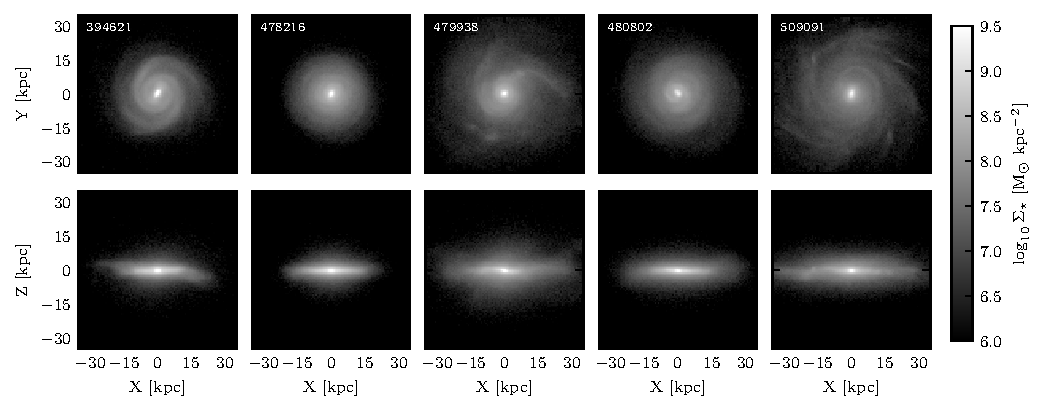
\includegraphics[width=\textwidth]{figure/ch4/galaxy_xyz_projection.pdf}
    \caption{Stellar mass surface density for five of the Milky Way analogs selected in \S~\ref{ch4:subsec:analog-selection} shown face-on (top) and edge-on (bottom) at $z=0$. The subfind IDs of each galaxy is annotated in the top row of panels, and distances are in physical kpc.}
    \label{ch4:fig:galaxy-surface-density}
\end{figure}

Before continuing on with sample selection, we describe here some steps we take to prepare subhalos for kinematic analysis. First, we determine the center-of-mass of each subhalo by applying the recursive shrinking-spherical-center algorithm described by \textcite{power03} to the star particles, shrinking the sphere by a factor 0.9 (i.e. each new radius is 0.9 times the size of the previous) each iteration and halting when fewer than 100 particles are enclosed. From particle velocities we subtract the mass-weighted mean velocity of all star particles within one stellar half-mass radius, $r_{h}$, of the center of the subhalo. We then rectify the galaxy to the vector described by the total angular momentum of the star particles between $0.5-2$ times $r_{h}$ from the center.

Now returning to analog selection, since our simple selection for Milky Way analogs by their stellar mass is agnostic towards the morphology of the chosen galaxies, we further pare down the sample by examining the relative fraction of spherical (bulge and halo) and disky stellar components. We assess these quantities using the orbit circularity, defined as $\eta = J_{z}/J_\mathrm{circ}(E)$ the specific angular momentum about the z-axis divided by the specific angular momentum of a circular orbit with a given energy $E$. We determine $J_\mathrm{circ}(E)$ empirically by relying on the fact that at any energy the maximum allowed angular momentum is that of a circular orbit. We therefore calculate the maximum angular momentum for particles in 100 bins evenly spanning the minimum to maximum energies, and fitting to this trend a 1-D spline, which gives $J_\mathrm{circ}(E)$.

% \james{Maybe need to present some argument about why removing galaxies with excess spheroid is important?}

To proxy the disk we consider the fraction of stars within $2r_{h}$ with circularity greater than 0.7, subtracting the fraction of stars within $2r_{h}$ with circularity less than $-0.7$ (hereafter disk fraction). For the bulge or spherical component we use twice the fraction of stars within $2r_{h}$ with circularity less than 0 (hereafter bulge fraction). Figure~\ref{ch4:fig:bulge-disk-decomposition} shows these quantities for the 46 stellar mass-selected analogs. The marginal distribution of these quantities reveals two populations, a concentrated group with spheroid and disk fractions between $0.1-0.4$ and $0.4-0.8$ respectively, alongside a second group or extended tail of the distribution at larger spheroid fraction and lower disk fraction. Visual examination reveals that many of the galaxies in the group with higher spheroid fraction are undergoing mergers at the present day.

The population with higher disk fraction is broadly consistent with the Milky Way, which has an approximate stellar bulge mass fraction of 0.3 and disk mass fraction of about 0.7 \parencite[see][and references therein]{bland-hawthorn16}. This set of mass fractions, with fiducial uncertainties of 0.05, is shown on Figure~\ref{ch4:fig:bulge-disk-decomposition}. Note that the population of Milky Way analogs does not overlap this locus, and we do not expect it to since the Milky Way mass fraction values are determined in a much more systematic, tailored manner, whereas our metrics are more approximate.

We extract the 30 galaxies with disk fraction greater than 0.35 and spheroid fraction less than 0.45, and remove the 16 other galaxies from the sample. There is good overlap between our sample and the sample of TNG50 Milky Way analogs compiled by \textcite{tng50_mw_pillepich23}. All but one of our analogs is also found in their much larger (numbering 198) sample of analogs which is defined by a much broader stellar mass range ($10^{10.5} \sim 3\times10^{10} < M_{\star} / {\rm M}_{\odot} < 10^{11.2} \sim 1.5\times10^{11}$), as well as an isolation criterion and a less stringent morphology criterion based on the aspect ratios of the stellar light distribution.

\begin{figure}
    \centering
    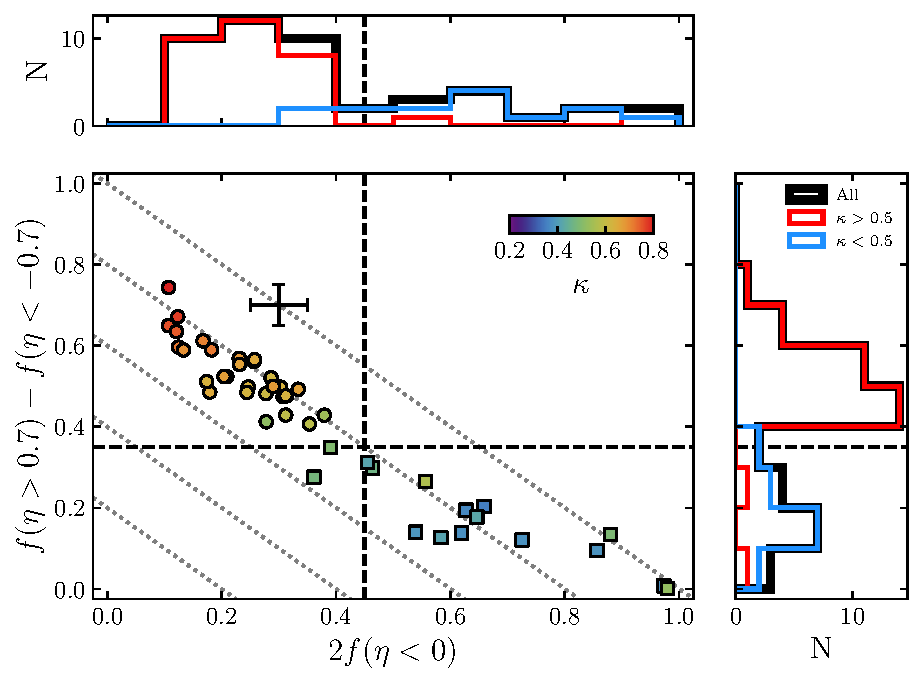
\includegraphics[width=0.8\textwidth]{figure/ch4/spheroid_disk_decomposition.pdf}
    \caption{The disk proxy (fraction of circularities above 0.7 minus the fraction below $-0.7$) as a function of the spheroid proxy (twice the fraction of circularities below 0) for the 46 mass-selected analogs. Histograms in the right and top panels show the margins of each of these quantities respectively. Circles are analogs included in the sample based on cuts, and squares are analogs excluded from the sample. The colorscale shows the fraction of energy in ordered rotation, $\kappa$. The dashed lines show the cuts adopted to separate galaxies with Milky Way-like spheroid and disk fractions. Those remaining in the sample are circles, and those removed from the sample are crosses. The set of error bars in the top-left quadrant shows the approximate bulge and disk fraction of the Milky Way.}
    \label{ch4:fig:bulge-disk-decomposition}
\end{figure}

We compare this selection using proxied disk and spheroid fractions to other types of selections which can discriminate between galaxies with disky and spheroidal stellar components. First we consider the fraction of energy in ordered rotation \parencite{sales10,correa17}, defined as 
\begin{equation}
    \label{ch4:eq:kappa}
    \kappa = \frac{ \sum_{i}^{N} m_{i} (J_{z,i}/R_{i})^{2}  }{ \sum_{i}^{N} m_{i} v_{i}^{2} }\,,
\end{equation}
\noindent where $J_{z,i}$ are specific angular momenta about the disk axis, $R_{i}$ are cylindrical radii, $v_{i}$ is the velocity magnitude for each particle, and $m_{i}$ are particle masses. We compute $\kappa$ for all star particles within $2r_{h}$, and report the values as the colorscale in Figure~\ref{ch4:fig:bulge-disk-decomposition}. It is clear when examining this figure that $\kappa$ trends strongly with more Milky Way-like disk and spheroid fraction. Indeed when examining $\kappa$ alone we find two groups at approximately $\kappa=0.4$ and $\kappa=0.7$, and the sample very neatly divides at $\kappa=0.5$, with only two excluded analogs lying at slightly higher values, and all included analogs lying at higher values.

We also examine the bulge and disk fractions reported by \textcite{du20} based on the approach presented by \textcite{du19}. These authors perform an unsupervised decomposition of IllustrisTNG galaxies into traditional stellar components in the space of orbital circularity $\eta$ and normalized energy $E/\max(\vert E \vert)$. We find the galaxies remaining in our sample tend to have disk fraction $>0.4$ and bulge fraction between 0.05 and 0.4, while the galaxies removed from the sample have slightly higher bulge fractions between 0.1 and 0.5, but much lower disk fractions $<0.5$. Each of these two subsequent lines of analysis on our sample strengthen our confidence in the way in which we select our final analog sample. 

\subsection{Identification of major mergers}

For each Milky Way analog we identify major mergers of interest using merger trees generated with the \texttt{SUBLINK} \parencite{rodriguez-gomez15} algorithm. In this work we are interested only in remnants which represent large accretion events for two reasons: first these remnants will be similar to the most thoroughly studied of the Milky Way remnants, and second these will have sufficient particle numbers such that kinematic modelling is possible. One has multiple options to define merger significance, it could be by present-day stellar or dark matter mass, or it could be by mass ratio at the epoch of the merger event. We elect to use the latter, since it allows for study of merger remnants from a variety of epochs on a more even footing.

We broadly follow the approach of \textcite{rodriguez-gomez16} when selecting merger remnants based on mass ratio. First, we consider the stellar mass ratio of the secondary versus the primary (the Milky Way analog). We choose the stellar mass ratio as opposed to the dark matter mass ratio because the star particles are more strongly bound to both the secondary and primary in the time leading up to the coalescence of the secondary, and so suffer less from pathological swapping and misplacing of particles by the \texttt{SUBFIND} algorithm during these close encounters. We also choose to measure the mass ratio at the time when the mass of the secondary reaches its largest value. We record all mergers with mass ratio greater than 20:1 at the corresponding time of largest secondary stellar mass. In this way we select 116 major mergers. An overview of their stellar and dark matter masses and primary-to-secondary mass ratios, as well as the redshift of the merger is shown in Figure~\ref{ch4:fig:merger-params}.

\begin{figure}
    \centering
    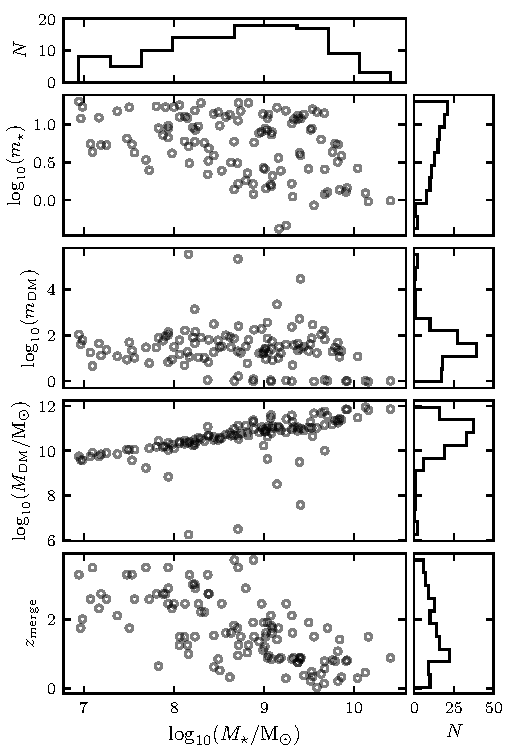
\includegraphics[width=0.6\textwidth]{figure/ch4/merger_params.pdf}
    \caption{The physical properties and merger attributes of identified major mergers. The four main panels show, in descending order, primary-to-secondary stellar ($m_{\star}$) and dark matter ($m_{\rm DM}$) mass ratio, secondary dark matter mass, and merger redshift, all as functions of the secondary stellar mass. The mass ratios are computed at the time of maximum secondary stellar mass. The merger redshift is defined by the snapshot where the secondary is last recorded as an independent subhalo. The top-most panel shows the distribution of secondary stellar masses, and the four right-most panels show the distributions of each of the dependent parameters shown in the main panels.}
    \label{ch4:fig:merger-params}
\end{figure}

\section{Fitting distribution function models to data}
\label{ch4:sec:fitting-distribution-functions}

Here we first describe the three DF models that we use, and then the methods used to fit them to N-body remnant data. Throughout this section and the next we will on multiple occasions bin the data to compute velocity dispersions as well as the orbital anisotropy. In general we bin star particles according to the following scheme, unless specified otherwise. Bins for each remnant are of variable width and always contain $\min[500,N/10]$ particles, where $N$ is the total number of particles. In other words we use 500 particles per bin unless there are fewer than 5000 particles in the remnant ($\sim 4\times10^{8}$~\Msun\ remnant stellar mass), in which case we use 10 bins. The innermost bin edge always lies at $\max[\epsilon_{\star},\min(\{ r_{i} \})]$ where $\{r_{i}\}$ is the set of star particle galactocentric radii. All bins contain the same number of star particles, and particles outside the final bin edge are ignored. Our goal in using a fixed-number binning approach is to ensure that dispersions and anisotropies have consistent uncertainties, which depend on the number of star particles used for the computation.

\subsection{The constant-anisotropy and Osipkov-Merritt distribution functions}
\label{ch4:subsec:distribution-function-models}

The first model we consider is spherical with constant anisotropy, and takes the form
\begin{equation}
    \label{ch4:eq:constant-anisotropy-df}
    f(\mathcal{E},L) = L^{-2\beta} f_{1}(\mathcal{E})\,.
\end{equation}
\noindent Here the relative energy $\mathcal{E} = \Psi - \frac{1}{2}v^{2}$ is a function of $\Psi = -\Phi-\Phi(\infty)$, the negative of the gravitational potential offset to be 0 at infinity, as well as the velocity $v$. $L$ is the total angular momentum, and the parameter $\beta$ is the anisotropy, which is given as
\begin{equation}
    \label{ch4:eq:beta}
    \beta = 1- \frac{\sigma^{2}_{\theta} + \sigma^{2}_{\phi}}{2\sigma^{2}_{r}}\,,
\end{equation}
\noindent where $\sigma_{[\theta,\phi,r]}$ are the spherical velocity dispersions in the polar, azimuthal, and radial directions respectively. $\beta$ has the domain $(-\infty,1]$, with negative values corresponding to a tangentially biased system, a value of 0 corresponding to an isotropic or ergodic (i.e. the DF depends only on energy) system, and positive values corresponding to a radially biased system. Finally, the function $f_{1}$ relates the tracer density of the DF to the underlying potential. For ergodic ($\beta=0$) DFs $f_{1}$ can be solved by a simple integral inversion \parencite{eddington16}, however for non-zero $\beta$ the calculation is more involved. For more information see \textcite{cuddeford91}, \textcite{an06}, chapter 4.3 of \textcite{binney08}, and Appendix A of \textcite{lane22} which specifically describes the implementation of this DF we use in \texttt{galpy} \parencite{bovy15}.

The second model we consider is typically independently attributed to \textcite{osipkov79} and \textcite{merritt85}, and is spherical with an anisotropy which approaches $\beta = 0$ at small radii, increasing with radii until it approaches $\beta = 1$ at large radii, reflecting the behaviour of many real galaxies. This DF takes the simple form
\begin{equation}
    \label{ch4:eq:osipkov-merritt-df}
    f(\mathcal{E},L) = f(Q)\,,
\end{equation}
\noindent where
\begin{equation}
    \label{ch4:eq:osipkov-merritt-Q}
    Q = \mathcal{E} - \frac{L^{2}}{2r_{a}^{2}},
\end{equation}
\noindent is a pseudo-energy which is constructed from the relative energy $\mathcal{E}$ and the total angular momentum $L$ scaled by a characteristic radius $r_{a}$. $f(Q)$ is computed via an integral inversion, in a manner similar to the ergodic and constant-anisotropy distribution functions. The anisotropy of the Osipkov-Merritt model varies as a function of spherical radius $r$, taking the form
\begin{equation}
    \label{ch4:eq:beta-osipkov-merritt}
    \beta(r) = \frac{r^{2}}{r^{2} + r_{a}^{2}}\,.
\end{equation}
\noindent From which it is clear that $\beta(0)=0$, that $\beta(r_{a})=1/2$, and that $\beta$ tends towards 1 as $r \rightarrow \infty$.

A final DF that we consider is a linear superposition of standard Osipkov-Merritt DFs with differing $r_{a}$ values. These types of DFs were first described by \textcite{merritt85}, who noted that they allow for a wider range of anisotropy and velocity dispersion profiles than the standard single-$r_{a}$ form. A two-component Osipkov-Merritt superposition DF is defined as
\begin{equation}
    \label{ch4:eq:osipkov-merritt-superposition-df}
    f(Q) = k_\mathrm{om}f_{1}(Q) + (1-k_\mathrm{om})f_{2}(Q),
\end{equation}
\noindent where $f_{1}$ and $f_{2}$ are two standard Osipkov-Merritt DFs described by $r_{a,1}$ and $r_{a,2}$ and $k_\mathrm{om}$ is the fraction of the DF corresponding to $f_{1}$. It is possible to explore a broader family of superposition DFs with additional linear components, or even with functional definitions for the weights corresponding to different $r_{a}$, but for simplicity we consider only models with two components here. Each component will also have the same density profile which is specified by the best-fitting density profile.

\subsection{The rotating DF prescription}
\label{ch4:subsec:rotating-df-prescription}

A final ingredient we add to our DFs is rotation about the galactic z-axis, which is implemented following the prescription of \textcite{binney14d} \parencite[see also][for an equivalent implementation using constant-anisotropy DFs]{deason11}. Consider that a DF $f(\mathbf{I})$, which is a function of some conserved quantities $\mathbf{I}$ such as energy and angular momentum or actions, can be split into an even (non-rotating) and odd (rotating) DF as 
\begin{equation}
    \label{ch4:eq:even-odd-df}
    f(\mathbf{I}) = (1-k_\mathrm{rot})f_{+}(\mathbf{I}) + k_\mathrm{rot}f_{-}(\mathbf{I})\,,
\end{equation}
\noindent where $k_\mathrm{rot}$ is the fraction of the DF which is rotating. If $f_{+}(\mathbf{I})$ is one of the DF models listed above, the odd portion of the DF is defined as
\begin{equation}
    \label{ch4:eq:rotating-df-kernel}
    f_{-}(\mathbf{I}) = \tanh \big( L_{\mathrm{z}}/\chi \big) f_{+}(\mathbf{I})\,,
\end{equation}
\noindent where $L_{\mathrm{z}}$ is the angular momentum about the galactic z-axis, and $\chi$ is the angular momentum scale at which rotation becomes significant. Since this prescription for rotation does not change the overall angular momentum $L$, or the energy $\mathcal{E}$ it can be applied to either the constant-anisotropy DF or the Osipkov-Merritt without changing the fundamental nature of the DF.

\subsection{Fitting distribution functions to data}
\label{ch4:subsec:fitting-constant-anisotropy-osipkov-merritt-dfs}

The procedure to fit the constant anisotropy and both standard and superposition Osipkov-Merritt DFs is similar. We consider that the required ingredients to construct these DFs are the gravitational potential $\Phi$, the density profile of the tracer $\rho$, and a parameter which specifies the anisotropy: $\beta$ for the constant-anisotropy DF, $r_{a}$ for the Osipkov-Merritt DF, and $\{ r_{a,1},r_{a,2},k_\mathrm{om} \}$ for the superposition Osipkov-Merritt DF. As mentioned above, these models are computationally expensive to work with we therefore build the DF from each of these individual components, which are tractable to obtain on their own, as opposed to fitting the entire model to data all at once. 

We begin by considering the host gravitational potential $\Phi$. Since each of the DF models rely on an explicitly spherical underlying potential (they are functions of $\mathcal{E}$ and total $L$), we construct a sphericalized representation of the mass profile of each host galaxy at $z=0$ to act as the potential. We first determine the enclosed mass profile $M(r)$ as a function of radius for all baryonic and dark matter particles. We then spline-interpolate the radial force $F_{r} = -\frac{G M(r)}{r^{2}}$ on a logarithmically-spaced grid from the minimum to maximum radius of all particles considered. From this representation the potential is computed trivially as the integral of the spline.

The second step is to fit the density of the tracer population, in this case each individual merger remnant. For the density profile we elect to use a two-power model which takes the form
\begin{equation}
    \label{ch4:eq:two-power-spherical-density}
    \rho_{\rm rem}(r) = \frac{ \rho_{\mathrm{r},0} }{ (r/r_{s})^{\alpha_{1}} (1+r/r_{s})^{\alpha_{2}-\alpha_{1}} }\,,
\end{equation}
\noindent where $\rho_{0}$ is the amplitude, $\alpha_{[1,2]}$ are the inner and outer power law indices, and $r_{s}$ is the scale radius marking the transition between the two power law indices. We choose this profile due to its flexibility, specifically in being able to realistically describe remnants such as GS/E, which is known to have a shallow inner density profile which steepens at a characteristic radius \parencite[e.g.][]{han22,lane23}.

We fit this density profile to data using a likelihood-based framework, which we describe here very generally. At the core is Bayes theorem
\begin{equation}
    \label{ch4:eq:bayes-theorem}
    p(\mathbf{\Theta} \vert \{ \mathbf{X} \} ) \propto p( \{ \mathbf{X} \} \vert \mathbf{\Theta} ) p( \mathbf{\Theta} )
\end{equation}
\noindent where $\mathbf{\Theta}$ are a vector of model parameters to be determined and $\{ \mathbf{X} \}$ is a vector of data in a relevant coordinate frame. The posterior, $p(\mathbf{\Theta} \vert \{ \mathbf{X} \} )$, is of interest and is determined by the likelihood $p( \{ \mathbf{X} \} \vert \mathbf{\Theta} )$, hereafter $\mathcal{L}(\mathbf{\Theta})$, and any priors $p( \mathbf{\Theta} )$.

As befits our data, we employ the log-likelihood for the Poisson point process
\begin{equation}
    \label{ch4:eq:loglikelihood-poisson-point-process}
    \log \mathcal{L}(\mathbf{\Theta}) \propto  \sum_{i=0}^{N} \rho(\mathbf{X}_{i}; \mathbf{\Theta}) - \int_{\mathrm{V}} \rho(\mathbf{X}; \mathbf{\Theta} ) \mathrm{d}V
\end{equation}
\noindent where here $\mathbf{X}_{i}$ are coordinate vectors for individual data points. The integral in the likelihood is over the volume $V$ encompassed by the particles.

% which may either be restricted to some small part of space around each galaxy or infinite when the density profile has a bounded mass.

For each remnant we use all star particles tagged in the last snapshot as a part of the subhalo which contributed to the merger. We place the following domain priors on the fitting of each remnant: $\alpha_{2} > \alpha_{1}$, $\alpha_{2} > 0$, and $\max[\epsilon_{\star},\min(\{ r_{i} \})] < r_{s} < \max(\{ r_{i} \})$. Notably we do not enforce that $\alpha_{1} > 0$ which may seem a natural requirement. While testing we found that some remnants have density profiles which genuinely decrease in density near $r=0$, and others which are very flat near $r=0$ and require a negative value for $\alpha_{1}$ to sufficiently flatten the two-power profile to obtain a good fit. We place logarithmic priors on the values of $\alpha_{2}$ and $r_{s}$ to encourage them not to diverge towards large values (even though $r_{s}$ is bounded).

We draw samples from the posterior using the affine-invariant Markov chain Monte Carlo (MCMC) ensemble sampler of \textcite{goodman10} implemented in \texttt{emcee} by \textcite{foreman-mackey13}. We initialize our walkers in a small volume of parameter space around a set of parameters determined by optimizing the log-likelihood using the conjugate direction method of \textcite{powell64}. We use 100 walkers and draw 2000 samples per walker, discarding 500 per walker as burn-in. We examine by-eye the posterior distributions to ensure that they are well-converged. We do not observe any bimodal or otherwise unduly complicated posterior distributions, and therefore define the best-fitting parameters as the median of the distribution, with the uncertainties being defined as the 16th and 84th percentiles.

Next we determine the anisotropy-specifiying parameters for the DFs, either the single value for the constant-anisotropy DF, $r_{a}$ for the Osipkov-Merritt DF, or $\{ r_{a,1},r_{a,2},k_\mathrm{om} \}$ for the superposition Osipkov-Merritt DF. To obtain these parameters we directly fit the anisotropy, defined according to equation~\eqref{ch4:eq:beta}, as a function of radius. We compute the anisotropy by binning all star particles according to the prescription at the beginning of \S~\ref{ch4:sec:fitting-distribution-functions} and computing the radial, azimuthal, and polar velocity dispersions. Note that we also test whether using the mean-square velocities, as opposed to the velocity dispersions, affects our fits, and find minimal impact. This is important for remnants with net rotation as the dispersions are not equivalent to the mean-squares.

We define a simple Gaussian objective function $\mathcal{O}$ for binned data to find the best-fitting parameters
\begin{equation}
    \label{ch4:eq:beta-objective-function}
    \log \mathcal{O}(\Theta) = \sum_{i=0}^{N} -\frac{ \big[ \beta_\mathrm{M}(r_{i};\Theta) - \beta_{i} \big]^{2} }{2/m_{i}}\,,
\end{equation}
\noindent where $\Theta$ is the parameters which specify the anisotropy, $\beta_\mathrm{M}(r_{i};\Theta)$ is the model anisotropy evaluated at a radial bin center $r_{i}$, $\beta_{i}$ are the remnant velocity dispersions computed as described above, and $m_{i}$ is the total amount of mass in stars per bin (even though the number of particles per bin is constant their mass can vary). 

The model anisotropy is trivial for the constant-anisotropy DF, and for the standard Osipkov-Merritt DF it is given by equation~\eqref{ch4:eq:beta-osipkov-merritt}. For the superposition Osipkov-Merritt DF determining the model anisotropy is not so simple, and computation of the individual velocity dispersion profiles for each component DF is necessary. The radial and tangential ($\sigma_{t} = \sqrt{\sigma_{\phi}^{2} + \sigma_{\theta}^{2}}$) velocity dispersions for the superposition Osipkov-Merritt model are given by \textcite{merritt85} as
\begin{equation}
\label{ch4:eq:superposition-osipkov-merritt-dispersions}
\begin{split}
    \sigma_{r}^{2} = &\ k_\mathrm{om} \sigma_{r,1}^{2} + (1-k_{\mathrm{om}}) \sigma_{r,2}^{2} \\      
    \sigma_{t}^{2} = &\ k_\mathrm{om} \sigma_{t,1}^{2} + (1-k_{\mathrm{om}}) \sigma_{t,2}^{2}\,, \\      
\end{split}
\end{equation}
where dispersions with subscripts 1 and 2 are computed from the Osipkov-Merritt DFs with $r_{a,1}$ and $r_{a,2}$ respectively.

Again due to the fact that computing DF moments is expensive, it is intractable to obtain these dispersion profiles on-the-fly when fitting. We navigate this issue by computing $\sigma_{r}$ and $\sigma_{t}$ on a grid of $r$ and $r_{a}$ for each remnant. We consider 10 values of $r_{a}$ logarithmically spaced from $10^{-1}$~kpc to $10^{2.5}$~kpc and 20 values of $r$ logarithmically spaced from $\max[\epsilon_{\star},\min(\{ r_{i} \})]$ to $\max(\{ r_{i} \})$. Using interpolation we can then quickly compute velocity dispersions, and then the anisotropy using equation~\eqref{ch4:eq:beta}, for any $r_{a}$ at any radius while fitting. We examine the velocity dispersion grids by-eye, and find them to appear well-behaved and smooth, such that we are comfortable using interpolation in this situation.

To fit we follow the same approach as used for the density profile above, first optimizing the objective function to obtain initial conditions and then using MCMC to sample the posterior. Again, we examine our posteriors and find no complicated features or multimodalities and so define the best-fitting anisotropy, $r_{a}$, and $\{ r_{a,1},r_{a,2},k_\mathrm{om} \}$ for each model respectively as the medians of the respective posterior distributions.

% (either a constant or given by equation~\eqref{ch4:eq:beta-osipkov-merritt})

%  \james{Here is use $k$ but in some of the plots and internally I use $f_{rot}$, I actually like $k$ better and think I'll change the plots to match.}

Finally we fit for the rotating component of the DF. We determine this in a DF-independent manner by fitting for the asymmetry between positive and negative values of $L_{\mathrm{z}}$. For the prescription outlined in \S~\ref{ch4:subsec:rotating-df-prescription} the asymmetry between positive and negative values of $L_{\mathrm{z}}$ is
\begin{equation}
    \label{ch4:eq:Lz-anisotropy}
    A(L_{\mathrm{z}}) = \frac{k_\mathrm{rot}}{2} \tanh(L_{\mathrm{z}}/\chi) + \frac{1}{2}\,.
\end{equation}
\noindent The asymmetry in $L_{\mathrm{z}}$ is computed for each remnant by evenly binning from $[-L_{\mathrm{z},80},L_{\mathrm{z},80}]$ where $L_{\mathrm{z},80}$ is the 80th percentile of $\lvert L_{\mathrm{z}} \rvert$ with a number of bins equal to the number of star particles divided by 20 (but no less than 50 bins). The asymmetry is computed as the number count in each bin divided by the sum of the number count in the bin and its complement (at opposite $L_{\mathrm{z}}$). When a bin and its counterpart at opposite $L_{\mathrm{z}}$ contain no star particles they are removed from consideration. 

We use the same objective function, equation~\eqref{ch4:eq:beta-objective-function}, as was used for the anisotropy data, however we replace the measured anisotropy in bins and predicted anisotropy with the measured and predicted $L_{\mathrm{z}}$ asymmetry, and change the mass term in the denominator to the mass in each $L_{\mathrm{z}}$ bin. We follow the same approach as was used to determine the best-fitting parameters for the anisotropy profile, again finding no complex features in the posteriors and therefore using the median $k_\mathrm{rot}$ and $\chi$ as the best-fitting parameters.

With all of the ingredients for our DFs determined individually we build each DF out of its constituent components by solving for $f_{1}(\mathcal{E})$, $f(Q)$, or $f_{1}(Q)$ and $f_{2}(Q)$ pursuant to the definitions in \S~\ref{ch4:subsec:distribution-function-models} and then applying the rotation prescription. Figure~\ref{ch4:fig:density-df-params} is a corner plot showing the best-fitting density profiles and DF properties derived in this section. Also shown are remnant stellar masses, merger stellar mass ratios, and merger redshifts for reference and comparison. In the top corner of each panel is an ellipse representing the covariance matrix of those parameters, with axis ratios being the ratios of the eigenvalues of the matrix, and the orientation set by the eigenvectors. For context, we show the properties of the GS/E remnant as a large purple circle in the background in relevant panels (i.e. where the properties of the remnant are known). We assume the following for GS/E: the anisotropy to be $\beta=0.9$ \parencite{belokurov18,lancaster19}; the inner and outer power laws to be $[1,4]$ with a break radius of 20~kpc \parencite[][]{han22,lane23}; the accretion redshift to be $z=2$ \parencite[see][]{mackereth19a,montalban21}; the stellar mass to be $3\times10^{8}$ \parencite[a value typical of recent findings;][]{mackereth20,han22,lane23}; and the stellar mass ratio to be 1:8 \parencite{lane23}. 

\begin{figure}
    \centering
    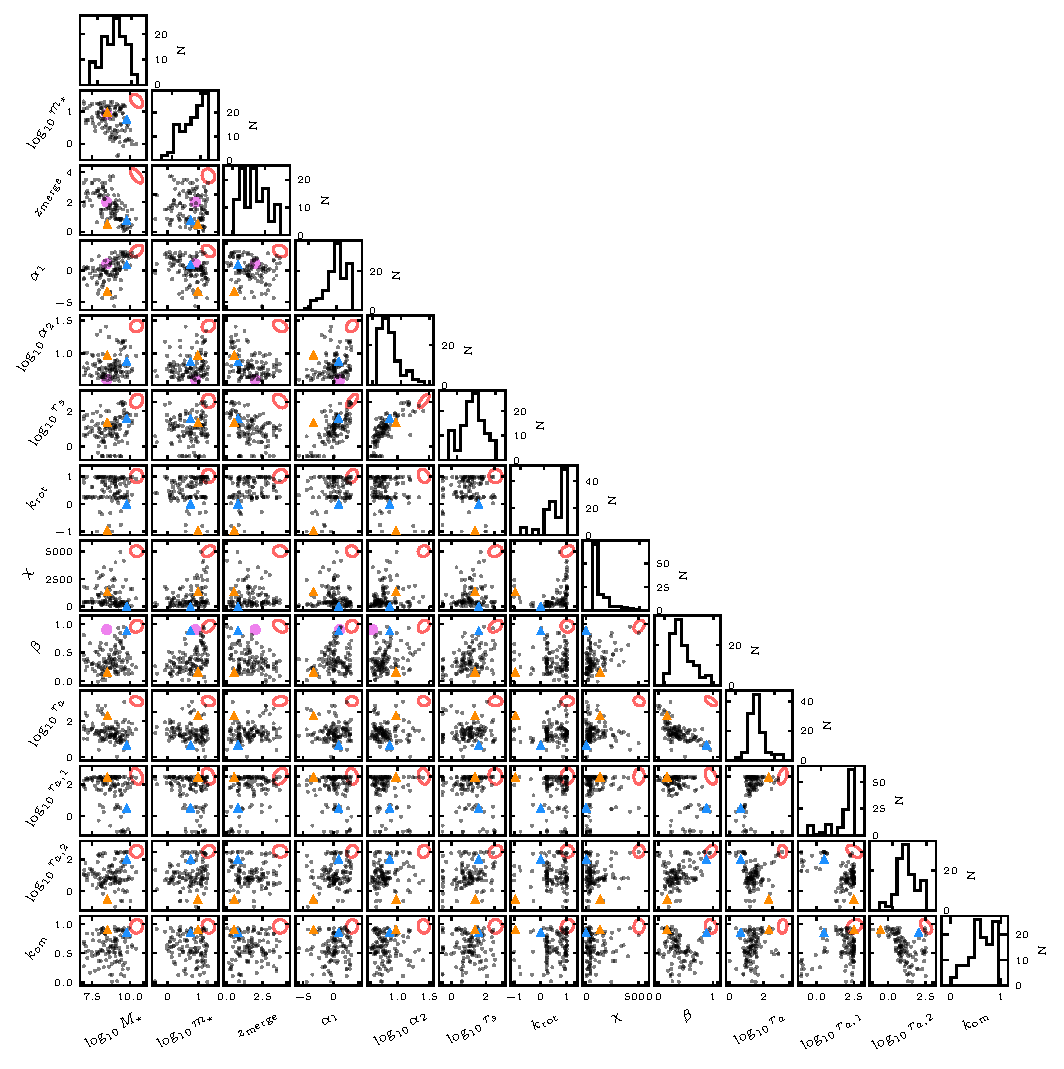
\includegraphics[width=\textwidth]{figure/ch4/density_df_params.pdf}
    \caption{Corner plot summarizing the properties of the 116 major mergers as well as the best-fitting density profile and DF parameters for each of the three classes of DF considered. Shown first are the merger properties: log secondary stellar mass in \Msun, log major-to-minor stellar mass ratio, and merger redshift. Following that are the remnant density profile parameters: inner power law index, log outer power law index, and log of the scale radius in kpc. Then is the rotational fraction and rotation scale parameter. Finally are the DF parameters: anisotropy for the constant-anisotropy DF, log scale radius for the single Osipkov-Merritt model in kpc, log scale radii for the combined Osipkov-Merritt models in kpc, and the mixture fraction for the combined Osipkov-Merritt model. The red ellipse in the corner of each panel is a representation of the covariance matrix for those parameters. The purple circle is the approximate properties of the GS/E remnant (see text for details). The blue and orange triangles are the remnants chosen to be GS/E and Sequoia case studies respectively.}
    \label{ch4:fig:density-df-params}
\end{figure}

A number of noteworthy trends present themselves here beyond the relations among stellar mass, mass ratio, and merger redshift already apparent in Figure~\ref{ch4:fig:merger-params}. First we see that remnant stellar mass correlates with inner power law index $\alpha_{1}$ such that more massive remnants tend to have steeper inner density profiles. Remnant anisotropy does not exhibit a strong correlation with remnant stellar mass, however high-anisotropy remnants do tend to have moderate to large stellar masses $\gtrsim 10^{8.5}$~\Msun. But the remnants with the largest stellar masses $\gtrsim 10^{9.5}$~\Msun\ actually tend to have modest anisotropies of $0 < \beta < 0.5$. Remnant anisotropy more strongly correlates with merger stellar mass ratio such that more even mergers $(m_{\star} \sim 1-5)$ tend to me more ergodic than uneven mergers $(m_{\star} \sim 10-20)$. This is an interesting observation given the current prevailing paradigm that the Milky Way was subject to a recent ($z_\mathrm{merger} \sim 2$), significant merger, the remnant of which is the GS/E population in the stellar halo which exhibits a high-degree of radial anisotropy. Remnant stellar mass finally appears to correlate with $r_{a}$, however since $r_{a}$ and $\beta$ are intimately linked this is similar to noting that stellar mass correlates with anisotropy.

Merger redshift tends to correlate with quantities which also trend with stellar mass such (i.e. density profile parameters and anisotropy) since these two quantities are intimately linked. In a hierarchical Universe all structures, including smaller dwarf galaxies, grow with time and therefore mergers are larger at later times. But in addition to the quantities which also trend with stellar mass, merger redshift appears to trend with remnant net rotation such that early mergers typically (always for $z>2.5$) co-rotate with $k_\mathrm{rot} > 0$, while only late-time mergers exhibit $k_\mathrm{rot} < 0$. This is likely a reflection of the fact that early mergers play a key role in setting the overall angular momentum in a growing galaxy, and therefore early mergers will tend to match the angular momentum of the primary at $z=0$. Of note is the general lack of retrograde mergers, only 9 out of 116 major mergers have $k_\mathrm{rot} < 0$.

Among the density profile parameters $\alpha_{1}$, $\alpha_{2}$, and $r_{s}$ all correlate. Given the correlations with stellar mass noted above, this indicates that more massive mergers tend to have steep inner power laws and strong breaks at large radii, while lower mass mergers tend to have shallow inner power laws with weak breaks and shallow outer power laws. Constant anisotropy $\beta$ is strongly anticorrelated with $r_{a}$, which is understandable given that smaller $r_{a}$ implies that the Osipkov-Merritt DF will have a high anisotropy over a larger radial range. There are also relations between the three superposition Osipkov-Merritt parameters and other parameters, but to note these is mostly to revisit the already noted trends including the other anisotropy parameters.


% \subsection{The action-based distribution function}
% \label{ch4:subsec:fitting-action-dfs}

% \james{This section will probably be in the submitted paper}

\section{Assessment and comparison of distribution functions}
\label{ch4:sec:assessment-comparison-distribution-functions}

Two tasks now lie before us. The first is to first determine whether these DFs provide a satisfactory model for the remnant N-body data. The second is to gauge whether one DF is superior to the others, and if so under which conditions or for which type of remnants. To tackle the first question we will compare the N-body data to each best-fitting DF model in a self-consistent manner. For the second question we will compare the DF models to each other in the context of the underlying N-body data.

When directly comparing models with N-body data to answer the first question posed above we will proceed in a numerical manner. This is facilitated by drawing samples from each of the best-fitting DFs for each remnant to act as a representation of the DF. The advantage of sampling each DF, as opposed to computing the metrics we will summarize in the next section in a different numerical manner, is that sampling intrinsically accounts for shot noise and allows for error estimation in the metrics through bootstrapping. For each remnant, and each DF fit to that remnant, we draw a number of samples equal to the number of N-body star particles in the remnant from the respective DF. We sample radii between the minimum and maximum N-body particle radii. For more information on how we generate samples from DFs see Appendix~A4 of \textcite{lane23}.

\subsection{Two case studies: GS/E and the Sequoia}
\label{ch4:subsec:case-studies}

Before moving to a broader comparison of all remnants, which will necessitate generating summary statistics that may cloud the specific details of any individual remnant, we first examine two case studies. We select remnants matched to two of the best-studied stellar halo populations in the Milky Way: GS/E and Sequoia. GS/E is a comparatively massive remnant with high anisotropy and low net rotation \parencite{belokurov18,helmi18}, while Sequoia is thought to be a lower mass remnant with high net rotation in the direction opposite disk rotation \parencite{myeong19,naidu20}. We record the properties of the selected merger remnant analogs in Table~\ref{ch4:tab:merger-case-study-properties}. For more information about merger tree identifiers see the Illustris-TNG documentation\footnote{\url{https://www.tng-project.org/data/docs/specifications}}. The properties of the chosen mergers are highlighted in Figure~\ref{ch4:fig:density-df-params}.

\begin{table}
    \centering
    \caption{Key identifying characteristics of the GS/E and Sequoia case study merger remnants. SID is short for SubfindID, and is the identification for a specific subhalo within the TNG50-1 simulation merger tree at a given snapshot (here the $z=0$ snapshot). MLPID is short for MainLeafProgenitorID, which is the unique identification of the branch of the merger tree corresponding to the secondary. The notation $0^N$ indicates $N$ repeating zeros, employed for brevity. $M_{\star}$ is secondary stellar masses and $m_{\star}$ is the primary to secondary mass ratio. Both are reported at the epoch where the secondary reaches its maximum stellar mass. $z_\mathrm{merger}$ is the redshift of the last snapshot where the secondary appears as a distinct subhalo.}
    \begin{tabular}{lcc}
        Property & GS/E & Sequoia \\
        \hline \\
        Primary $z=0$ SID    & 522530 & 518682 \\
        Secondary MLPID      & 9601673 &  $20^{6}280^{3}41936$ \\ % 20000002800041936 \\ %
        $M_{\star}$ [\Msun]  & $6.2\times10^{9}$ & $3.2\times10^{8}$ \\
        $m_{\star}$          & 5.6:1 & 9.6:1 \\
        $z_{\mathrm{merge}}$ & 0.79 & 0.52 \\
    \end{tabular}
    \label{ch4:tab:merger-case-study-properties}
\end{table}

To select a GS/E analog we examine remnants with $\beta > 0.8$ (numbering 6 total), and choose one with stellar mass of $\approx 6\times10^{9}$~\Msun\ and anisotropy of $\beta=0.88$, which was deposited in a 6:1 stellar mass ratio merger (30:1 dark matter mass ratio) at $z \approx 0.8$. In choosing the GS/E analog we focus most on anisotropy, attempting to match the value for GS/E of $\sim 0.9$. The stellar mass of GS/E has been subject to a wide range of estimates, spanning nearly two decades from $10^{8}$ to $10^{10}$~\Msun, however more direct measurements of the density profile of GS/E have tended to settle on a lower stellar mass range of $1.5-7.2\times10^{8}$~\Msun\ \parencite{mackereth20,han22,lane23}. These estimates typically correspond with a total mass ratio for the merger in the range of 1:4-1:10 (normally assuming a GS/E merger epoch of $z\approx2$). So the mass ratios are in broad agreement with estimates for GS/E, while the total stellar mass is on the high-end of estimates. The accretion epoch for GS/E is thought to be 7-11~Gyr ago ($z \sim 0.8-2.4$), and so this merger is on the very lowest end of that range. This partially explains the higher total stellar mass. Only one of the candidate remnants with high-anisotropy merged at $z>1$, however it only has a present-day stellar mass of only $\sim 10^{7}$~\Msun, much too low to be considered an appropriate analog for GS/E.

For the Sequoia analog we examine strongly counter-rotating remnants with $k < -0.5$ (also numbering 6 total). We select one with a strong degree of rotation, $k=-0.96$, and stellar mass $3\times10^{8}$, which is comparable to current estimates \parencite{myeong19,matsuno19,naidu20}. The remnant has low anisotropy ($\beta=0.14$), and merged comparatively late ($z=0.52$) compared with the Sequoia remnant which is though to have been deposited between $z=1-2$ \parencite{kruijssen20}. The typical angular momentum $L_\mathrm{z}$ for Sequoia ranges between $1-3 \times 10^{3}$~kpc~km~s$^{-1}$, and our chosen remnant spans a slightly lower range with 16th, 50th, and 84th percentile $L_\mathrm{z}$ of $-2.3,-1.1$ and $0.2\times 10^{3}$~kpc~km~s$^{-1}$.

Figure~\ref{ch4:fig:case_study_beta_vdisp} shows the velocity dispersions and anisotropy profiles for the GS/E (top row) and Sequoia (bottom row) case studies. For each quantity the N-body data is shown in black, with the DF sample realizations shown in blue (constant-anisotropy), red (Osipkov-Merritt), and orange (superposition Osipkov-Merritt). Here we also point out a minor pathology in our fitting procedure. The rotating DF prescription for strongly rotating remnants (i.e. our Sequoia analog) tends to decrease $\sigma_{\phi}$ in DF samples, since $L_\mathrm{z}$ values cluster (at positive or negative values depending on the sense of rotation). While the absolute values of $L_{z}$ remain the same, and therefore overall distribution of orbit shapes is conserved, the concentration of $L_{z}$ to positive or negative values decreases the spread in tangential velocity, which decreases $\sigma_{\phi}$. This effect can be seen in Figure~\ref{ch4:fig:case_study_beta_vdisp} where the sample anisotropies seem slightly larger than would fit the data. This effect is minor, however, and its occurrence here represents its largest effect.

Now returning to the analysis of the analogs. for the GS/E analog we see that the constant-anisotropy DF correctly specifies the characteristically large anisotropy found at large radii ($10-100$~kpc), but at radii less than 10~kpc the anisotropy profile softens until it approaches zero at the smallest radii. This results in an interesting interplay between the DFs, whereby the Osipkov-Merritt model more correctly models the lower anisotropy at small radii, but overestimates the anisotropy at large radii since the model always tends towards $\beta=1$. The constant-anisotropy model, on the other hand, more accurately tracks the large anisotropy at large radii, but obviously cannot accommodate the lowering in anisotropy at small radii. These differences are mirrored in the individual velocity dispersion trends, which also show each model performing well at either small or large radii. On the other hand this situation exemplifies the benefits of the superposition Osipkov-Merritt model, which is able to reproduce the anisotropy along with each velocity dispersion well at all radii.

\begin{figure}
    \centering
    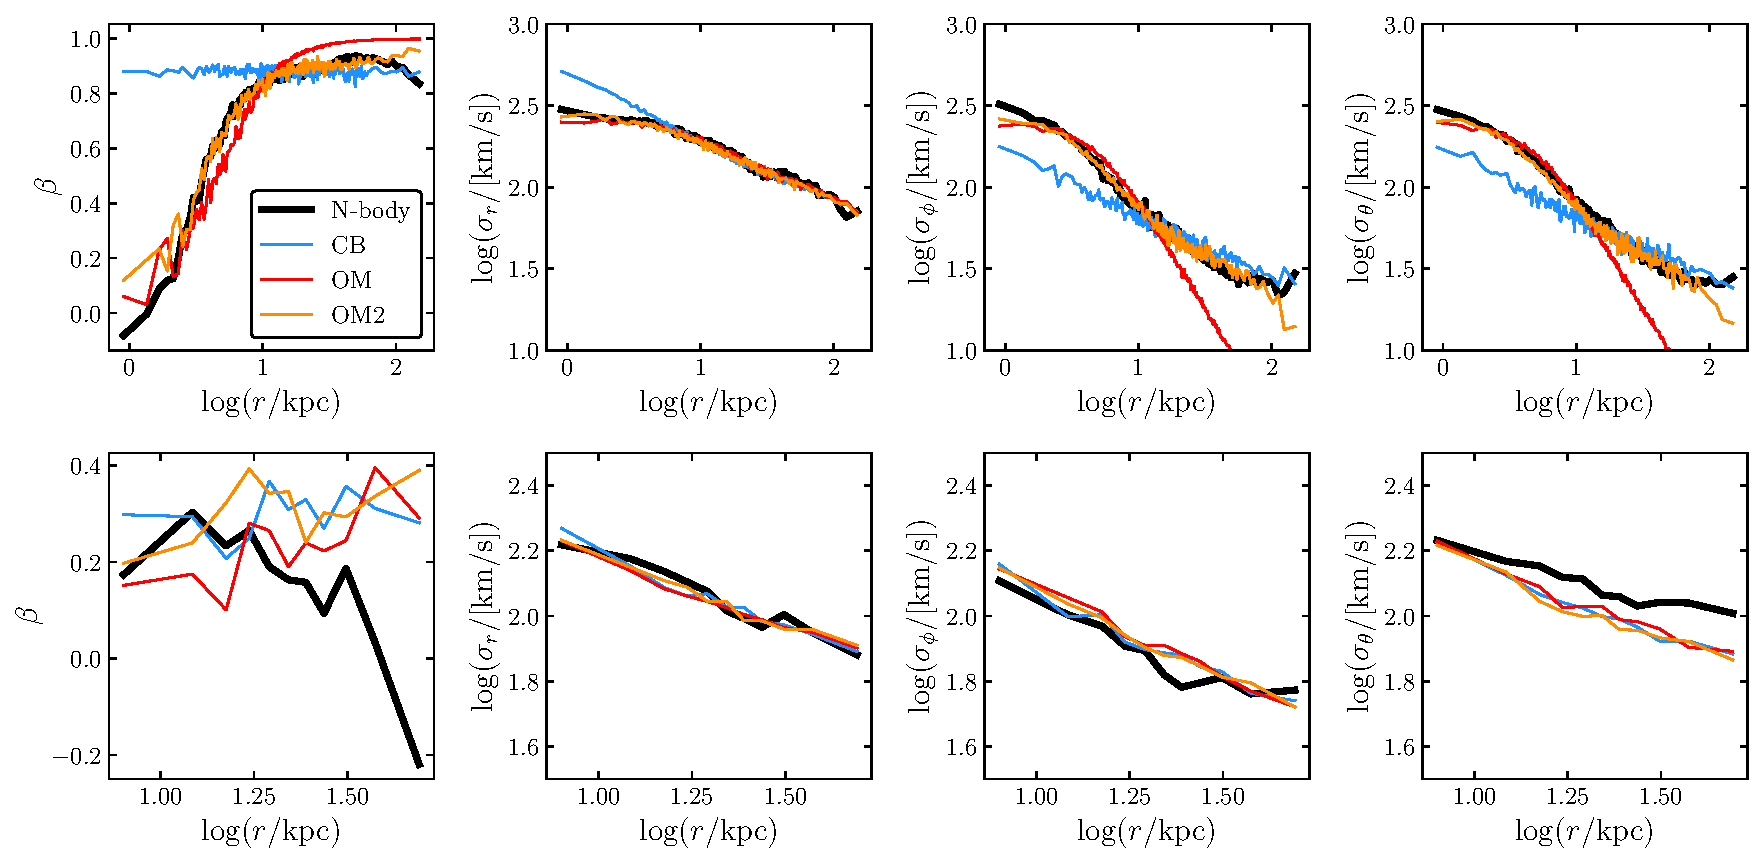
\includegraphics[width=\textwidth]{figure/ch4/beta_vdisp.pdf}
    \caption{Anisotropy and velocity dispersions for the two case studies from \S~\ref{ch4:subsec:case-studies}, the GS/E (top row) and Sequoia (bottom row). The columns, from left to right, show as functions of radius: anisotropy, radial velocity dispersion, azimuthal velocity dispersion, and polar velocity dispersion. In each panel the black curve shows the N-body data, and the blue, red, and orange curves show the samples from the best-fitting constant-anisotropy, standard Osipkov-Merritt, and superposition Osipkov-Merritt DFs respectively.}
    \label{ch4:fig:case_study_beta_vdisp}
\end{figure}

For the Sequoia analog, which has a much lower typical anisotropy of about 0.2, all models are able to reasonably capture the behaviour at all radii. For the Osipkov-Merritt DF the best-fitting $r_{a}$ is very large ($\sim 500$~kpc), which allows the anisotropy and velocity dispersion profiles to approach constant values. Note that this is only possible because the analog has a constant, yet low, value. Were the value to be much higher the Osipkov-Merritt model would struggle to replicate its constancy. Notably the tangential velocity dispersions are fit reasonably, despite the model rotation, although the fit is not as good as for the radial velocity dispersions.

Figure~\ref{ch4:fig:case_study_ELz} shows energy and $L_\mathrm{z}$ for the N-body data (black histogram), as well as the DF samples from the best-fitting models (histograms not shown). The energies for the N-body data are offset by the median energy of the particles within 5~per~cent of the stellar half-mass radius, calculated in the interpolated potential (the potential which governs the DFs) in order to bring the energies in line with the DF samples. A single contour is shown for each distribution, placed at the same density level for the N-body data as for the DF sample data (recall they have the same number of data points) in order to compare the distributions.

\begin{figure}
    \centering
    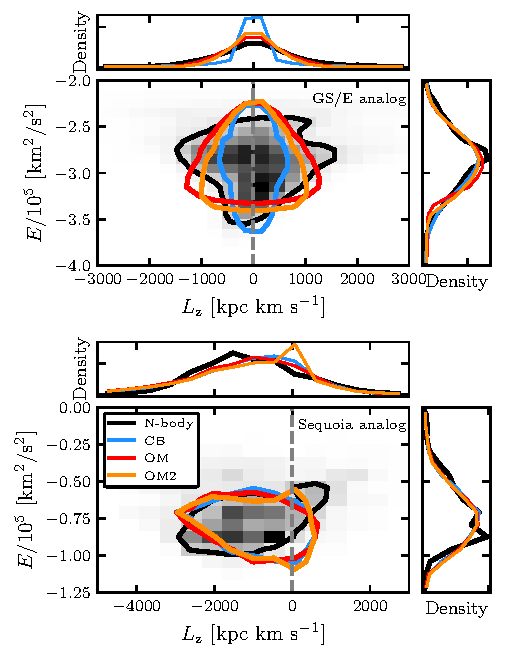
\includegraphics[width=0.6\textwidth]{figure/ch4/energy_Lz.pdf}
    \caption{Energy and z-axis angular momentum for the GS/E analog (top panels) and Sequoia analog (bottom panels). The black contours show the N-body data, while the blue, red, and orange contours show the samples from the best-fitting constant-anisotropy, standard Osipkov-Merritt, and superposition Osipkov-Merritt DFs respectively. The background histogram shows the binned N-body data. For each analog the N-body and DF samples contain the same number of data points, are binned identically, and the contours rest at the same levels. The smaller panels above and to the right of each primary panel show the density margins of the angular momentum and energy respectively, binned in the same manner as the primary panels.}
    \label{ch4:fig:case_study_ELz}
\end{figure}

For the GS/E analog the N-body data displays a downward-pointing triangular morphology, centered about $L_\mathrm{Z}=0$, which is typical for both the stellar halo in large, but also for individual accretion remnants. The constant-anisotropy DF spans a very narrow range of angular momenta, which reflects the fact that all orbits must have low $L_\mathrm{z}$ to enforce the high anisotropy at all radii. The Osipkov-Merritt samples display the opposite behaviour compared with the N-body data, where $L_\mathrm{z}$ tends to decrease with increasing energy, resulting in an upward-pointing triangular morphology. This can be understood in the context of the model, where the anisotropy at large radii (roughly equivalent to large energies) is high, therefore requiring angular momentum to be low. Conversely at small radii (roughly equivalent to low energies) the angular momentum spans a larger range since the anisotropy is low. The superposition Osipkov-Merritt model does not do much better than the standard Osipkov-Merritt, only taking a slightly narrower profile. Overall each model is able to appropriately capture the correct range of energies (about $10^{3}$~km$^{2}$~s$^{-2}$), and the Osipkov-Merritt models are able to appropriately capture the range of angular momentum (roughly $\pm 1500$~kpc~km~s$^{-1}$) unlike the constant-anisotropy model. But none of the models are able to replicate the specific upward-pointing triangular morphology exhibited by the N-body data.

For the Sequoia analog the story is broadly similar. Here, each model is able to correctly capture the locus of the N-body distribution in angular momentum, as well as the spread in energies. Their similarity in this regard is expected given that they share the rotational DF prescription. Along the same terms as Figure~\ref{ch4:fig:case_study_beta_vdisp}, each DF model has become similar in nature to fit the constant, low anisotropy, which is reflected in the similarity of their sample distributions. But the actual morphology of the N-body distribution, where energy decreases as angular momentum increases, is not well-fit by the DF samples, which exhibit the opposite trend. This trend exhibited by the DF samples is as-expected for low-anisotropy rotating models, whereby angular momentum is larger for orbits with larger energies. So perhaps this particular Sequoia analog defies these expectations, which could link back to the specifics of the merger.

To summarize this exercise, generally these simple DF models are able to accurately capture the broad strokes of the kinematics of N-body data to which they are fit: spans in energy and angular momentum, net rotation, and the magnitudes of the velocity dispersion profiles. But the specifics of the data are not well-fit, excepting the case of the superposition Osipkov-Merritt model GS/E analog anisotropy and dispersions, which are in good agreement. However, the detailed morphology in the energy-angular momentum plane is not captured well by any of the models.

\subsection{Metrics for DF assessment and comparison}

In this subsection we outline three metrics that we employ both for comparison among the best-fitting DFs, as well as comparison between N-body data and the samples representing the DFs. The first metric is based on the Jeans equation, and is constructed to gauge the suitability of the N-body data for equilibrium modelling. The second metric is a weighted comparison of velocity dispersion profiles, and the third metric uses the likelihood for the Poisson point process. These latter two are designed to determine which DF fits the data better, and to estimate whether the models fit the data well or poorly.

\subsubsection{The Jeans equation}
\label{ch4:subsubsec:jeans-equation}

The first metric we consider is based on the time-indepent Jeans equation in spherical coordinates
\begin{equation}
    \label{ch4:eq:jeans-equation-spherical}
    \frac{\mathrm{d} (\nu\,\overline{v^2_r})}{\mathrm{d} r} +\,\nu\,
    \left(\frac{\mathrm{d} \Phi}{\mathrm{d} r}+
    \frac{2\overline{v_r^2}-\overline{v_\theta^2}-\overline{v_\phi^2}}{r}\right) = 0\,,
\end{equation}
where $\nu$ is the number density of the tracer, $\overline{v^{2}}_{[r,\phi,\theta]}$ are the spherical mean-square velocities (equivalent to the squared velocity dispersions when the mean velocity in that dimension is zero), $\Phi$ is the underlying gravitational potential, and $r$ is the spherical radius. For steady-state spherical systems in equilibrium this equation is satisfied, and the right-hand-side is equal to zero. Computing this equation for a system in disequilibrium will result in a non-zero residual related to the time derivative of the DF. 

We can compute these terms in the spherical Jeans equation for our N-body data, and then examine the magnitude of the residual to gauge whether the remnant we are interested in appears to be in equilibrium or not. Since computation of the Jeans equation as laid out in equation~\eqref{ch4:eq:jeans-equation-spherical} is DF-independent, this does not allow us to make statements about how well each DF fits the data, but rather it may add crucial information about the state of equilibrium to inform our investigation of the merits of other DFs.

We first ``normalize'' the Jeans equation by dividing it by a characteristic term $\nu\overline{v^{2}_{r}}/r$ such that the equation and any residual is unitless. This allows us to compare residuals from different DFs on a more even footing. We hereafter refer to residuals of the Jeans equation normalized in this way as $\mathcal{J}$. We compute the terms of the Jeans equation numerically as follows. We first define a set of bins that will be used to compute the radial derivatives of $\nu \overline{v^{2}_{r}}$ and $\Phi$. These bins are defined as per the beginning of \S~\ref{ch4:sec:fitting-distribution-functions}. We then define a second set of bins for the undifferentiated terms $\nu$ and the anisotropy term within the brackets of equation~\eqref{ch4:eq:jeans-equation-spherical}. The edges for these bins are the bin centers for the radial derivative term bins. In this way each set of quantities is computed, and then the radial derivatives are evaluated numerically at positions corresponding to the bin centers for the undifferentiated quantities.

We are left with the residual of the Jeans equation computed on a radial grid. We compute two metrics to summarize the residuals, the first, $\overline{\mathcal{J}}$ is the mean of the residuals across all bins, weighting by the mass of stars in each bin (note that while each bin contains an equal number of star particles, the masses of the star particles can vary). The second, $\sigma(\mathcal{J})$, is the root-mean-square of $\mathcal{J}$ about $\overline{\mathcal{J}}$, also weighted by the mass of stars in each bin. We compute these quantities both for the stellar N-body data for each remnant, as well as the samples drawn from each best-fitting DF. Comparisons of the quantities $\overline{\mathcal{J}}$ and $\sigma(\mathcal{J})$ between N-body data and DF samples is shown in Figures~\ref{ch4:fig:J-mean} and \ref{ch4:fig:J-dispersion} respectively.

\begin{figure}
    \centering
    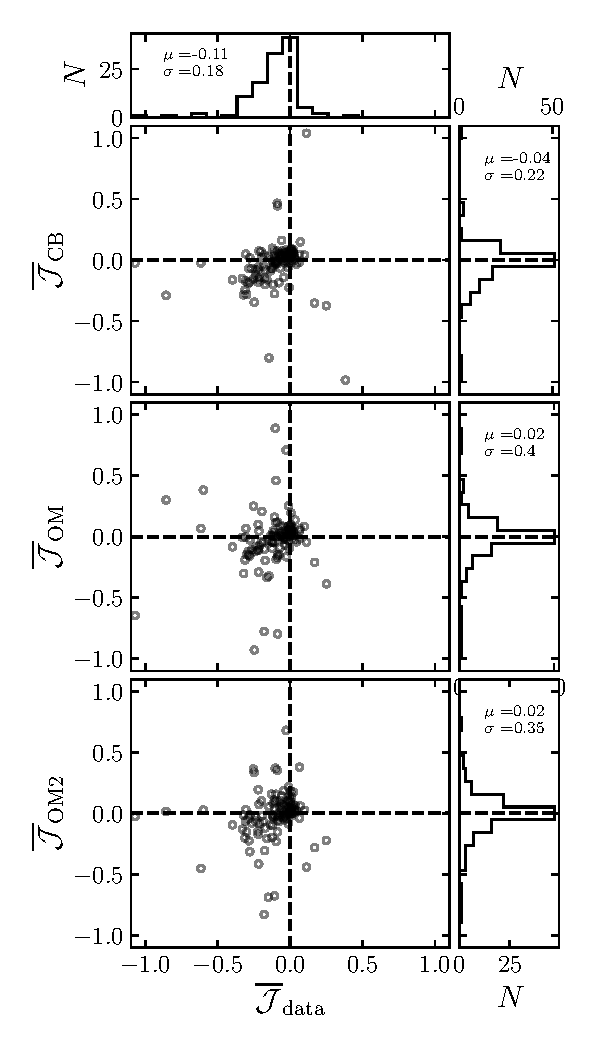
\includegraphics[width=0.6\textwidth]{figure/ch4/J_mean.pdf}
    \caption{Mass weighted mean $\mathcal{J}$ for each remnant studied in this work. Of the primary panels, the top shows the $\overline{\mathcal{J}}$ for the samples from the best-fitting constant beta DF versus the N-body data. The middle and bottom show the same but for the best-fitting Osipkov-Merritt and superposition Osipkov-Merritt DFs respectively. The dashed lines mark $\overline{\mathcal{J}}=0$. The top-most panel shows the marginal distribution of $\overline{\mathcal{J}}_{\mathrm{data}}$ and the two rightmost panels show the same for each set of DF samples respectively.}
    \label{ch4:fig:J-mean}
\end{figure}

\begin{figure}
    \centering
    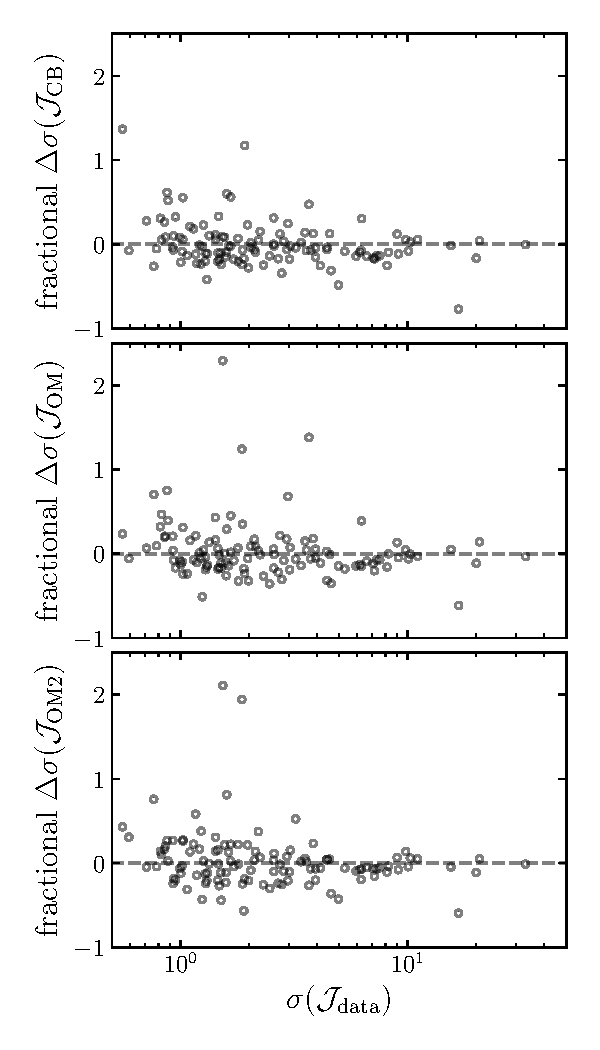
\includegraphics[width=0.6\textwidth]{figure/ch4/J_dispersion.pdf}
    \caption{Mass weighted $\mathcal{J}$ root-mean-square about $\overline{\mathcal{J}}$, $\sigma(\mathcal{J})$, for each remnant studied in this work. Each panel shows the fractional difference between the value of $\sigma(\mathcal{J})$ computed with the N-body particles and the corresponding DF sample. The panels are laid out in the same way as Figure~\ref{ch4:fig:J-mean}. The dashed line shows equal values of $\sigma(\mathcal{J})$ for N-body particles and DF samples.}
    \label{ch4:fig:J-dispersion}
\end{figure}

Since the samples drawn from the best-fitting DFs are in equilibrium and satisfy the spherical Jeans equation by definition, these two figures strongly suggest that the remnants we study are also in equilibrium. First, the values of $\overline{\mathcal{J}}$ for the DF samples shown in Figure~\ref{ch4:fig:J-mean} clearly cluster nicely around zero. We would not expect the values to be exactly zero even if the Jeans equation is satisfied since these are discrete realizations of the DF. The N-body data shows surprisingly comparable behaviour, with the data clustering about zero and exhibiting a scatter comparable to the DF sample data. The N-body data exhibits a slight negative bias, with a mean of $-0.13$, which is larger in magnitude than the means of the DF sample data. But this offset is smaller than the scatter in the distribution, which itself is not larger than the scatter for either set of DF sample data.

Figure~\ref{ch4:fig:J-dispersion} shows us that the magnitude of the scatter of the Jeans residual about the weighted mean is comparable for both N-body data and model. One might expect much larger values of $\sigma(\mathcal{J})$ for the N-body data, but this does not appear to be the case. Together, these data strongly suggest that it is reasonable to consider the N-body remnants to be in equilibrium, at least when compared with a comparable discrete realization of an explicitly time-independent DF. But using these results we cannot discern which DF provides a better fit to the data.

\subsubsection{Velocity dispersion profiles}
\label{ch4:subsec:velocity-dispersion-profiles}

The second metric we construct compares two sets of velocity dispersion profiles. The velocity dispersions for the N-body data are the same as was computed in \S~\ref{ch4:subsec:fitting-constant-anisotropy-osipkov-merritt-dfs}, via binning using the standard method. Velocity dispersion and anisotropy profiles for the model samples are computed similarly, using the same set of radial bins employed for the N-body data dispersions and anisotropies. The model sample velocity dispersions are not computed on their own grid because it is important for the metric we will now describe that the two sets of dispersions are on the same radial grid.

We then compute
\begin{equation}
    \label{ch4:eq:velocity-dispersion-delta}
    \delta = \frac{ \sum_{i}^{N} \big[ \lvert \sigma_{\rm data}(r_{i}) - \sigma_{\rm model}(r_{i}) \rvert m_{i} / s_{i} \big] }{ \sum_{i}^{N} m_{i} }\,,
\end{equation}
\noindent where $\sigma_{\rm data}$ are the velocity dispersions of interest ($r$, $\phi$, or $\theta$) for N-body data in radial bins centered on $r_{i}$, and $\sigma_{\rm model}$ are the sampled model velocity dispersions in the same bins. $s_{i}$ is the uncertainty in the N-body data velocity dispersions determined by taking the difference between the 84th and 16th percentiles of a sample of 100 bootstrap realizations of the velocity dispersion computation, with fixed bin sizes. Finally, $m_{i}$ is the mass of N-body star particles in each velocity dispersion bin, which is included because even though each bin contains the same number of particles they can have differing masses. In words this metric expresses the mass-weighted sum of the difference between N-body data and DF model sample velocity dispersions, scaled by the uncertainty in the N-body data.

We compute this metric, comparing N-body data and model samples for each DF, for radial, azimuthal, and polar velocity dispersions. We also compute the metric for the anisotropy profile in the same way, using equation~\eqref{ch4:eq:velocity-dispersion-delta} but substituting $\beta$ for $\sigma$. Since $\delta$ relies on binning it is sensitive to the discreet nature of the underlying data and resulting shot noise. We gauge the impact of this by computing $\delta$ for the DF samples against themselves using 100 bootstrap realizations. We record the median and central 68th percentile of the distribution of resulting values of $\delta$. This benchmark is the equivalent of an uncertainty limit on the value of $\delta$ and lends helpful context to the computed values in the sense that it represents the standard for a fit which is indistinguishable from the DF, given the number of data points.

Figure~\ref{ch4:fig:delta-comparison} compares the values of $\delta$ determined using the constant-anisotropy DFs and the Osipkov-Merritt DFs. Since larger values of $\delta$ indicate a larger deviation between N-body data and the respective DF samples, comparing $\delta$ in this way reveals whether one DF fits the data better than another. Also shown on Figure~\ref{ch4:fig:delta-comparison} are solid lines representing the median value of $\delta$ computed for the DF samples against themselves. Dashed lines are placed at 2 and 4 times this value. 

\begin{figure}
    \centering
    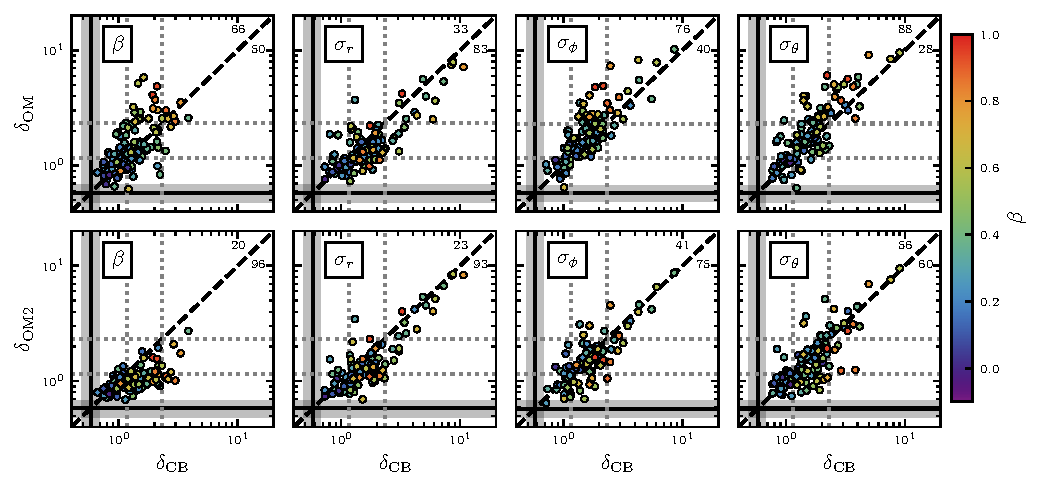
\includegraphics[width=\textwidth]{figure/ch4/delta_comparison.pdf}
    \caption{Comparison of $\delta$, the mass- and uncertainty-weighted deviation between data and model, calculated for $\beta$ and $\sigma_{[r,\phi,\theta]}$ (labelled, left to right). $\delta$ is determined using N-body data against the best-fitting DF samples. Delta is computed with the Osipkov-Merritt DF samples (top row) and linear combination Osipkov-Merritt DF samples (bottom row), and is shown against delta computed with the constant-anisotropy DF samples. The colour of the points shows the best-fitting constant anisotropy for the remnant. The solid lines and the surrounding fill show the median and central 68~per~cent interval of the bootstrapped computation of $\delta$ comparing each set of DF samples against itself. The dashed lines are placed at 2 and 4 times the median. The thick dashed line shows the 1:1 relation for reference. The numbers in the top-right corner of each panel show the number of points in the corresponding half of the figure defined by the 1:1 line.}
    \label{ch4:fig:delta-comparison}
\end{figure}

Examining this figure reveals some interesting trends. First is that $\delta$ computed using anisotropy profiles appears to favour the constant-anisotropy DF compared with the standard Osipkov-Merritt DF. Interestingly, this holds for both high- and low-anisotropy remnants. The velocity dispersion profiles show a different trend. For radial velocity profiles the Osipkov-Merritt profiles are favoured over the constant-anisotropy models. Whereas for the azimuthal and polar velocity dispersions the constant-anisotropy models are again favoured. This can be understood by referring back to Figure~\ref{ch4:fig:case_study_beta_vdisp}, which showed the velocity dispersion and anisotropy profiles for the GS/E and Sequoia case studies. There we saw that the radial velocity dispersion is well-fit over all radii by the Osipkov-Merritt model, and in particular it is able to capture the lower dispersions at small radii exhibited by both analog data. The Osipkov-Merritt DF struggles somewhat with the azimuthal and polar velocity dispersions, however, and cannot fully capture the overall anisotropy profile, especially for the highly anisotropic GS/E analog. The high-anisotropy remnant radial velocity dispersions appear to be better fit by the Osipkov-Merritt model, while the tangential velocity dispersions are not, which would track inline with this narrative.

On the other hand, the superposition Osipkov-Merritt DF again demonstrates its effectiveness as it exhibits values of $\delta$ which are much lower than the corresponding value for the constant-anisotropy DF across the board. The difference is most stark for the anisotropy and the radial velocity dispersion, and less for the tangential velocity dispersions. This can again be understood by referring to Figure~\ref{ch4:fig:case_study_beta_vdisp}, where we see that the superposition Osipkov-Merritt model is well-matched in all dispersions as well as anisotropy, in contrast to the constant-anisotropy model. These results clearly suggest that the superposition Osipkov-Merritt model should be favoured in comparison with the other two simpler models.

\subsubsection{Model log likelihoods}
\label{ch4:subsubsec:model-loglikelihoods}

The final metric we consider is a comparison of the total log likelihood of each model, computed via a modified version of equation~\eqref{ch4:eq:loglikelihood-poisson-point-process} where the density $\rho$ is replaced with the value of the corresponding DF, $f$, and the volume integral over configuration space is replaced with a volume integral over the relevant portion of 6D phase space (i.e. energy and angular momentum for the constant-anisotropy and Osipkov-Merritt DFs). We compute the total log likelihood using the N-body data for each DF ($\mathcal{L}_\mathrm{CB}$, $\mathcal{L}_\mathrm{OM}$, and $\mathcal{L}_\mathrm{OM2}$ for the constant-anisotropy, standard Osipkov-Merritt, and superposition Osipkov-Merritt models respectively).

\begin{figure}
    \centering
    \begin{subfigure}{0.8\textwidth}
        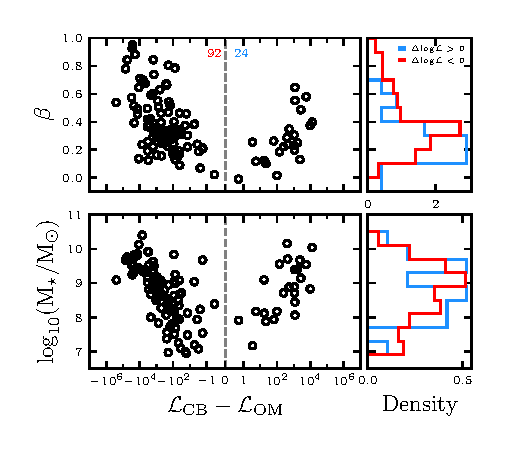
\includegraphics[width=0.8\textwidth]{figure/ch4/loglike_symlog_starmass_beta_comparison_cb_om.pdf}
        % \caption{Caption for Figure 1}
        % \label{ch4:fig:subfig1}
    \end{subfigure}
    \begin{subfigure}{0.8\textwidth}
        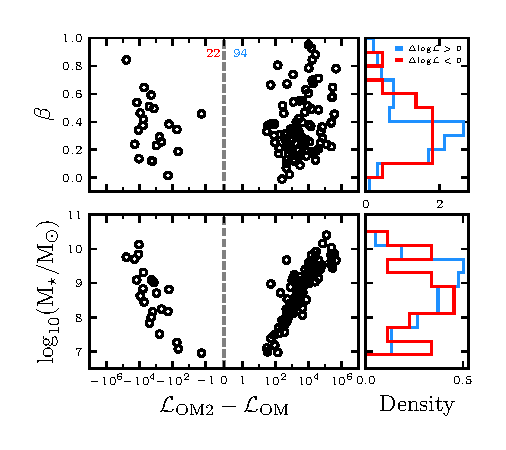
\includegraphics[width=0.8\textwidth]{figure/ch4/loglike_symlog_starmass_beta_comparison_om2_om.pdf}
        % \caption{Caption for Figure 2}
        % \label{ch4:fig:subfig2}
    \end{subfigure}
    \caption{Difference between the total log likelihood for the constant-anisotropy and Osipkov-Merritt models (top) and linear combination Ospikov-Merritt and standard Osipkov-Merritt (bottom). The axes are log-symmetric outside the range of -1 to 1, which is linear. Of each set of main panels, the top shows the difference in log likelihood as a function of anisotropy, while the bottom shows logarithmic stellar mass of the merger remnants. The right panels show the margins of the two quantities, split into groups where the difference in log likelihoods is greater than 0 and less than 0 (blue and red respectively) and is shown as density. Numbers in each of these samples are shown in blue and red on the main panels.}
    \label{ch4:fig:loglike-diff-beta-starmass}
\end{figure}

Figure~\ref{ch4:fig:loglike-diff-beta-starmass} shows the difference between the log likelihoods computed for the constant-anisotropy and Osipkov-Merrit DFs against the stellar mass of the remnant as well as the best-fitting constant anisotropy. The figure is replicated below it but for the standard Osipkov-Merritt against the superposition Osipkov-Merritt. The scale of each abscissa is log-symmetric, with the range from -1 to 1 being linear. The axes on the right-hand side show margins for the dependent quantities, split by whether $\Delta \mathcal{L}$ is greater than (blue) or less than (red) zero.

In regard to the top set of panels first, we see the majority of points lie on the left-hand side of the figure (92 versus 24) such that the likelihood for the Osipkov-Merritt model is greater than the constant-anisotropy model. Additionally, we see a trend such that the magnitude of the difference in the log likelihood tends to increase as both remnant mass and anisotropy increase. This is expected because the total log likelihood is a sum over all data points, and therefore the difference would be expected to increase with higher remnant mass. From a probabilistic perspective, more data points means higher confidence in the choice of one model over another. 

When examining the distributions split about $\mathcal{L}_\mathrm{CB} - \mathcal{L}_\mathrm{OM} = 0$ we see that for stellar mass they are broadly similar, with similar peaks and distribution widths. For anisotropy, however, it is clear that the distribution with $\mathcal{L}_\mathrm{CB} - \mathcal{L}_\mathrm{OM} < 0$ is peaked at higher values of anisotropy and has a tail which extends to the highest values of $0.8 < \beta < 1$. This indicates that while, in general, the likelihood analysis favours the Osipkov-Merritt model, it is specifically good at fitting remnants with high anisotropy.

Now moving on to the bottom set of panels, which compare standard Osipkov-Merritt against the superposition version of the DF. We see that here the majority of the points now lie on the right side of the figure, indicating preference for the superposition Osipkov-Merritt model. Again, we can investigate whether there are noteworthy trends with anisotropy by comparing the distributions divided by $\Delta \mathcal{L}$ in terms of anisotropy and stellar mass. We see less evidence here for a preference of the superposition DF among high-anisotropy remnants, although this conclusion is anchored by a single remnant with high-anisotropy which is better fit by the standard Osipkov-Merritt model. However it is clear that the distribution of points with $\Delta \mathcal{L} > 0$ is peaked around anisotropy of 0.4. This is expected given that standard Osipkov-Merritt can struggle to fit these intermediate anisotropy remnants, since its anisotropy prefers to toggle between $\beta = 0$ and $\beta = 1$, whereas the superposition model is able to plateau at intermediate values of $\beta$ over extended radial ranges.

One additional factor that we might consider here is whether or not the preference for the superposition Osipkov-Merritt DF over the standard version is driven by the increased number of parameters in the model (three versus one), which could hint at overfitting. We could consider that if we were to compare the Bayesian information criteria for each model it would be equivalent to adding a factor of $\sim \ln(N) k / 2$ to the difference of likelihoods already shown. Since the number of particles is the same in each instance, ranging roughly between $10^{4}-10^{6}$, and comparing $k=3$ and $k=1$ we have a range of about $9-14$ by which the value of $\Delta \mathcal{L}$ would be modified. Since most values of $\Delta \mathcal{L}$ for which the superposition DF is preferred are greater than $10^{2}$ and none are less than $10$ we can infer that we are not overfitting the problem by adding the two parameters for the superposition DF, and that the superposition DF should be genuinely preferred in most cases.

\section{Discussion}
\label{ch4:sec:discussion}

\subsection{The properties of merger remnants around Milky Way analogs}

While not the principal goal of this work, we have isolated and studied 116 merger remnants around 30 Milky Way analogs, fitting density profiles and distribution functions to them. We are able to report a large number of interesting relations, most of which are summarized in Figure~\ref{ch4:fig:density-df-params}. First, and certainly not unexpected in the context of $\Lambda$CDM is the relationship between merger redshift and secondary stellar mass, which is well-defined but too broad (about two decades in secondary stellar mass at fixed redshift and a factor of two in redshift at fixed secondary stellar mass) to be of much use in the context of inference in the Milky Way stellar halo. We also find that the only retrograde remnants $k_\mathrm{rot} < 0$ merged at redshifts $z<2.5$, and they are few in number (9 out of 116). We attribute this to the fact that early mergers are probably key in setting the angular momentum of the host galaxy, and therefore we would expect $k_\mathrm{rot} > 0$. But interestingly there is an overall lack of retrograde remnants even at redshifts $z<2.5$.

In regard to density profile parameters, we find that secondary stellar mass (and therefore merger stellar mass ratio since the Milky Way analog sample has a narrow range of stellar masses) correlates well with the inner slope of the remnant density profile: more massive remnants are steeper and less massive remnants shallower. Additionally the density profile parameters are well-correlated, such that remnants with steeper inner power laws have sharper transitions at larger radii when compared with remnants with shallow inner power laws which tend to also have shallow outer power laws. Connecting these trends with the relation between merger stellar mass and density profile parameters paints a broader picture. Lower mass remnants tend to have more uniform, shallow density profiles, while higher mass remnants have steeper density profiles with sharp cutoffs. These results are in line with the findings of \textcite{deason18}, who posit that the sharp density cutoff observed in the Milky Way stellar halo at $r \sim 20$~kpc is due to apocenter pileup of debris from a single large progenitor (in this case GS/E).

\subsection{A comparison of the DF models}

Our findings with respect to the three DFs studied in this work are mixed. First, we clearly see that the superposition Osipkov-Merritt DF model exhibits superior performance among the metrics by which we gauge DF performance as well as the more detailed investigations of the GS/E and Sequoia analogs. It is able to more accurately reproduce the velocity dispersion and anisotropy profiles of a wider range of remnants than either the constant-anisotropy or standard Osipkov-Merritt DF models. In addition the likelihood analysis clearly favours this model over the other two, even when taking into consideration the fact that it requires additional parameters.

But frustratingly none of the DF models were able to fully reproduce the observed morphology of either the GS/E or Sequoia analog remnants in the energy-angular momentum space. While each model was able to do a reasonable job of getting the locus and extent in energy and angular momentum of the N-body particles, they were unable to capture some of the semantic details in the distributions, such as the specific trends in the width and location of the distribution of angular momentum with varying energy. These failures highlight that while these models can be effective they are clearly limited. Coupling this with the fact that the DFs --- particularly the superposition Osipkov-Merritt DF -- can match the dispersions and anisotropy of the remnants well suggests that higher order moments of the DF could play an important role.

With this in mind it does appear to be the case that high-anisotropy remnants are better represented using the Osipkov-Merritt (and therefore naturally the superposition Osipkov-Merritt as well) model than the constant-anisotropy DF. The constant-anisotropy model substantially overpredicts the velocity anisotropy via the radial velocity dispersion at small radii. This leads to an overprediction for the density of stars with low angular momenta, as is seen in Figure~\ref{ch4:fig:case_study_ELz}. These observations are grounded in the mathematical behaviour of the constant-anisotropy models, which are known to be unstable for orbits with low tangential velocity \parencite{binney14d}.

Given the perceived shortcomings of the models considered in this work it is natural to consider other options. First and most significantly are action-based DFs such as the models put forward by \textcite{binney14d} and built upon by \textcite{posti15}. In these models the DF is a function of the actions $[J_{r},J_{z},L_{z}]$. They support a wide range of density profiles, and naturally incorporate variations in anisotropy, rotation, and flattening. The downside for these models is that the density profile and anisotropy are not directly specified. These models were recently used by \textcite{gherghinescu23} to model the whole halos of M31 analogs in the Auriga simulations. It will be useful in the future to consider a comparison between these action-based DFs and the Osipkov-Merritt DFs with which we have found the most success.

Another promising avenue for future study are neural network driven methods for obtaining DFs such as \textit{Deep Potential} described by \textcite{green23}. These approaches employ techniques such as normalizing flows, which are able to generate complex distributions via a series of well-defined transformations acting on a simple starting distribution such as a normal distribution. \textcite{green23} demonstrated that such models are able to recover known analytic DFs based on sampled phase space distributions. These techniques may be ideally suited for application to the complex phase space distributions we observe in the remnants in this work. Additionally, these types of models are likely easier to compute on-the-fly, an issue that we had to work around with our DFs by building them up piece-by-piece.

\subsubsection{The DF for GS/E}

Of great interest in the \textit{Gaia} era is to achieve detailed descriptions of the kinematics and dynamics of merger remnants in the Milky Way stellar halo so as to link them with their progenitors and the merger events which deposited them in the Galaxy. Density modelling has been successfully applied to this endeavour, both in regard to the stellar halo as a whole \parencite[e.g.][]{deason19,mackereth20} as well as individual remnants, particularly GS/E \parencite[e.g.][]{han22,lane23}. Our findings that the Osipkov-Merritt DFs are superior to the constant-anisotropy DF for modelling high-anisotropy remnants suggests that these DFs should be used to model GS/E in the future. Indeed, a promising future study would be to determine whether the radial velocity dispersion and the anisotropy drops for GS/E stars near the center of the galaxy, which would be consistent with our findings here for most high-anisotropy remnants. \textcite{lancaster19} studied the anisotropy of the stellar halo using BHB stars. They are unable to probe inwards of 10~kpc, but the anisotropy of the GS/E-like population in their study does appear to begin to drop slightly at these radii. \textcite{iorio21} use a much more numerous sample of RR Lyrae variables, and do indeed find that the anisotropy of their GS/E-like components does drop substantially within 5~kpc. The fraction of the halo composed of the GS/E-like component does also appear to drop in their data, however this may be a circular argument as if the true GS/E anisotropy does drop in the inner galaxy then the fraction would also drop if the GS/E component in these studies is defined as having high anisotropy. But disentangling potentially low-anisotropy GS/E stars in the inner galaxy from the old \textit{in-situ} stellar halo \parencite[e.g.][]{belokurov22,rix22}. Abundances may be crucial here, as the \textit{in-situ} halo should have different abundances, especially [Al/Fe] \parencite[see][]{belokurov22}, when compared with GS/E. Indeed, given that the chemical sequence of GS/E is now well-constrained with high-purity selections \parencite[e.g.][]{lane23} it should be possible to study its anisotropy profile using abundance-selected samples. If we assume that the anisotropy drops from 0.9 around $r=5$~kpc to about 0 in the center of galaxy then an Osipkov-Merritt profile with $2 < r_{a} < 4$~kpc should provide an adequate model for GS/E. 

\section{Summary and conclusions}
\label{ch4:sec:summary-conclusions}

In this work we study how well commonly used classes of DFs are able to describe merger remnants around Milky Way analogs in the IllustrisTNG simulations. We identify 116 major mergers, defined as having a mass ratio greater than 1:20, around 30 Milky Way analogs in the highest resolution TNG50 simulation run. We fit two-power spherical density profiles to remnants in addition to three classes of DF: the constant-anisotropy, standard Osipkov-Merritt, and superposition Osipkov-Merritt DFs.

We compare the DFs with N-body data by sampling from the DFs in a manner consistent with the N-body data and then generating a variety of summary statistics. We use the Jeans equation to gauge whether or not the remnants are in a state of dynamical equilibrium sufficient for modelling using DFs, and we find that they are. We compute the velocity dispersion and anisotropy profiles, and compare them for the N-body data and DF samples. We also compute the likelihoods for each model and compare them. Additionally, we examine two case studies corresponding to remnants matched to the well-studied GS/E and Sequoia populations in the Milky Way stellar halo.

Our main findings are summarized as follows:

\begin{enumerate}
    \item Remnants with higher degrees of anisotropy are more likely to exhibit sharp breaks in their density profiles, and the steepness of the break correlates with the anisotropy. Remnant anisotropy also correlates with remnant stellar mass. This reinforces observational evidence that apocenter pileup of a single large progenitor is responsible for the sharp break in the density of the Milky Way stellar halo.
    \item The remnants that we study appear, to a good approximation, to be in equilibrium, at least when benchmarked against representative DF samples.
    \item The DF models we consider are able to capture the correct locus and spread in energies and angular momenta for remnants with a variety of properties. Additionally, the magnitudes of the velocity dispersion profiles are well-matched to N-body data. The specific morphology of the remnants in energy-angular momentum space, as well as their velocity dispersion and anisotropy profiles, was not always well-matched by the best-fitting DFs.
    \item We find clear evidence that highly anisotropy stellar populations with $\beta > 0.8$, such as GS/E, are better modelled using the standard, or better the superposition, Osipkov-Merritt DF as opposed to the constant-anisotropy DF. While these remnants may have high average anisotropy, the profiles nearly always become more ergodic in the center of the Galaxy. We estimate that an Osipkov-Merritt profile with a scale radius of 2-4~kpc would provide a reasonable DF model for GS/E.
\end{enumerate}

In general our results were inconclusive with regards to providing a clear set of criterion to decide whether to use the constant-anisotropy or Osipkov-Merritt DF. We do see good evidence that high-anisotropy remnants are better-modelled using the Osipkov-Merritt DF. These remnants typically have radial velocity dispersion and anisotropy profiles which soften at small radii to lower anisotropy, behaviour which is better captured by the Osipkov-Merritt DFs compared with the constant-anisotropy DFs. We therefore leave this as a principle conclusion, and otherwise recommend that with regards to other remnants that one proceed on a case-by-case basis. We do find that superposition Osipkov-Merritt DFs are able to replicate a wide variety of anisotropy profiles, and so may be the most generally applicable. In conclusion, We hope that this study provides useful insight for a future in which much of the stellar halo has been explored and the task turns to detailed modelling.

% \section*{Acknowledgements}

% % We first thank the referee for their comments, which have certainly improved the quality of the manuscript. 

% JMML and JB acknowledge financial support from NSERC (funding reference number RGPIN-2020-04712) and an Ontario Early Researcher Award (ER16-12-061). We are very greatful to Ted Mackereth, who helped to conceptualize this project.

%%%%%%%%%%%%%%%%%%%%%%%%%%%%%%%%%%%%%%%%%%%%%%%%%%
% \section*{Data Availability}

% The IllustrisTNG simulations used in this article are publicly available at \url{https://www.tng-project.org/data/}.

%%%%%%%%%%%%%%%%%%%% REFERENCES %%%%%%%%%%%%%%%%%%

% The best way to enter references is to use BibTeX:

% \bibliographystyle{mnras}
% \bibliography{manuscript} % if your bibtex file is called example.bib

% %%%%%%%%%%%%%%%%%%%%%%%%%%%%%%%%%%%%%%%%%%%%%%%%%%

% %%%%%%%%%%%%%%%%% APPENDICES %%%%%%%%%%%%%%%%%%%%%

% \appendix

% \section{A toy model for interpreting Jeans residual summary statistics}
% \label{ap:jeans-residual-toy-model}



%%%%%%%%%%%%%%%%%%%%%%%%%%%%%%%%%%%%%%%%%%%%%%%%%%


% Don't change these lines
% \bsp	% typesetting comment
% \label{lastpage}
% \end{document}

% End of mnras_template.tex


% Chapter 5 - Conclusion
% \chapter{Conclusion}

\input{}

% Appendix
\appendix

% Backmatter & bibliography
\backmatter
\printbibliography[heading=bibintoc]

% End
\end{document}
